% ********************************** PhD Thesis  *****************************
% This is the PhD thesis of Mario G. Bejarano M.
% Note reference page layout \textwidth = 15.74 \textheight = 22.27
%\documentclass[a4paper,12pt,times,oneside,draft]{Classes/PhDThesisPSnPDF}
\documentclass[a4paper,12pt,times,numbered, draft,index]{Classes/PhDThesisPSnPDF}

% ******************************************************************************
% ******************************* Class Options ********************************
% *********************** See README for more details **************************
% ******************************************************************************

% `a4paper'(The University of Cambridge PhD thesis guidelines recommends a page
% size a4 - default option) or `a5paper': A5 Paper size is also allowed as per
% the Cambridge University Engineering Deparment guidelines for PhD thesis
%
% `11pt' or `12pt'(default): Font Size 10pt is NOT recommended by the University
% guidelines
%
% `oneside' or `twoside'(default): Printing double side (twoside) or single
% side.
%
% `print': Use `print' for print version with appropriate margins and page
% layout. Leaving the options field blank will activate Online version.
%
% `index': For index at the end of the thesis.	
%
% `draftclassic': For draft mode without loading any images (same as draft in book)
%
% `draft': Special draft mode with line numbers, images, and water mark with
% timestamp and custom text. Position of the text can also be modified.
%
% `abstract': To generate only the title page and abstract page with
% dissertation title and name, to submit to the Student Registry
%
% `chapter`: This option enables only the specified chapter and it's references
%  Useful for review and corrections.
%
% ************************* Custom Page Margins ********************************
%
% `custommargin`: Use `custommargin' in options to activate custom page margins,
% which can be defined in the preamble.tex. Custom margin will override
% print/online margin setup.
%
% *********************** Choosing the Fonts in Class Options ******************
%
% `times' : Times font with math support. (The Cambridge University guidelines
% recommend using times)
%
% `fourier': Utopia Font with Fourier Math font (Font has to be installed)
%            It's a free font.
%
% `customfont': Use `customfont' option in the document class and load the
% package in the preamble.tex
%
% default or leave empty: `Latin Modern' font will be loaded.
%
% ********************** Choosing the Bibliography style ***********************
%
% `authoryear': For author-year citation eg., Krishna (2013)
%
% `numbered': (Default Option) For numbered and sorted citation e.g., [1,5,2]
%
% `custombib': Define your own bibliography style in the `preamble.tex' file.
%              `\RequirePackage[square, sort, numbers, authoryear]{natbib}'.
%              This can be also used to load biblatex instead of natbib
%              (See Preamble)
%
% **************************** Choosing the Page Style *************************
%
% `default (leave empty)': For Page Numbers in Header (Left Even, Right Odd) and
% Chapter Name in Header (Right Even) and Section Name (Left Odd). Blank Footer.
%
% `PageStyleI': Chapter Name next & Page Number on Even Side (Left Even).
% Section Name & Page Number in Header on Odd Side (Right Odd). Footer is empty.
%
% `PageStyleII': Chapter Name on Even Side (Left Even) in Header. Section Number
% and Section Name in Header on Odd Side (Right Odd). Page numbering in footer


% ********************************** Preamble **********************************
% Preamble: Contains packages and user-defined commands and settings
% ******************************************************************************
% ****************************** Custom Margin *********************************

% Add `custommargin' in the document class options to use this section
% Set {innerside margin / outerside margin / topmargin / bottom margin}  and
% other page dimensions
\ifsetCustomMargin
  \RequirePackage[left=37mm,right=30mm,top=35mm,bottom=30mm]{geometry}
  \setFancyHdr % To apply fancy header after geometry package is loaded
\fi

% Add spaces between paragraphs
%\setlength{\parskip}{0.5em}
% Ragged bottom avoids extra whitespaces between paragraphs
\raggedbottom
% To remove the excess top spacing for enumeration, list and description
\usepackage{enumitem}
\setlist[enumerate,itemize,description]{topsep=0em}

% *****************************************************************************
% ******************* Fonts (like different typewriter fonts etc.)*************

% Add `customfont' in the document class option to use this section

\ifsetCustomFont
  % Set your custom font here and use `customfont' in options. Leave empty to
  % load computer modern font (default LaTeX font).
  %\RequirePackage{helvet}

  % For use with XeLaTeX
  %  \setmainfont[
  %    Path              = ./libertine/opentype/,
  %    Extension         = .otf,
  %    UprightFont = LinLibertine_R,
  %    BoldFont = LinLibertine_RZ, % Linux Libertine O Regular Semibold
  %    ItalicFont = LinLibertine_RI,
  %    BoldItalicFont = LinLibertine_RZI, % Linux Libertine O Regular Semibold Italic
  %  ]
  %  {libertine}
  %  % load font from system font
  %  \newfontfamily\libertinesystemfont{Linux Libertine O}
\fi

% *****************************************************************************
% **************************** Custom Packages ********************************

% ************************* Algorithms and Pseudocode **************************

%\usepackage{algpseudocode}


% ********************Captions and Hyperreferencing / URL **********************

% Captions: This makes captions of figures use a boldfaced small font.
\RequirePackage[footnotesize,bf]{caption}

\RequirePackage[labelsep=space,tableposition=top]{caption} 
\renewcommand{\figurename}{Figure} %to support older versions of captions.sty

%Chapter fancy title
\usepackage[Lenny]{fncychap}


% *************************** Graphics and figures *****************************

%\usepackage{rotating}
%\usepackage{wrapfig}

% Uncomment the following two lines to force Latex to place the figure.
% Use [H] when including graphics. Note 'H' instead of 'h'
\usepackage{float}
\restylefloat{figure}

% Subcaption package is also available in the sty folder you can use that by
% uncommenting the following line
% This is for people stuck with older versions of texlive
%\usepackage{sty/caption/subcaption}
\usepackage{subcaption}
\captionsetup[sub]{font=footnotesize,labelfont={bf,sf}}

%This allows to create image placeholder with a dummy image.
\newcommand{\dummyfig}[1]{
  \centering
  \fbox{
    \begin{minipage}[c][0.33\textheight][c]{0.5\textwidth}
      \centering{#1}
    \end{minipage}
  }
}



\usepackage{layouts}

% ********************************** Tables ************************************
\usepackage{booktabs} % For professional looking tables
\usepackage{multirow}
\usepackage{tabu}
\usepackage{rotating} % For rating tables
%\usepackage{array}
%\usepackage{multicol}
%\usepackage{longtable}
%\usepackage{tabularx}



% *********************************** SI Units *********************************
\usepackage{siunitx} % use this package module for SI units
\DeclareSIUnit{\sample}{S}
\DeclareSIUnit{\beats}{beats}
\DeclareSIUnit{\bfv}{\ml\per\min 100\ml}
\DeclareSIUnit{\mArms}{\milli\ampere{}_{RMS}}
\DeclareSIUnit{\uArms}{\micro\ampere{}_{RMS}}
\sisetup{separate-uncertainty,multi-part-units = single 
         ,exponent-to-prefix = true
         ,zero-decimal-to-integer}%


%Definition of tagaddtext for the units in the equation
\makeatletter
\providecommand\add@text{}
\newcommand\tagaddtext[1]{%
	\gdef\add@text{#1\gdef\add@text{}}}% 
\renewcommand\tagform@[1]{%
	\maketag@@@{\llap{\add@text\quad}(\ignorespaces#1\unskip\@@italiccorr)}%
}
\makeatother

% ************************ Support th notation *********************************
\usepackage[super]{nth}						% Support for the number notation

% ******************************* Line Spacing *********************************

% Choose linespacing as appropriate. Default is one-half line spacing as per the
% University guidelines

%\doublespacing
 \onehalfspacing
% \singlespacing


% ************************ Formatting / Footnote *******************************

% Don't break enumeration (etc.) across pages in an ugly manner (default 10000)
%\clubpenalty=500
%\widowpenalty=500

%\usepackage[perpage]{footmisc} %Range of footnote options


% *****************************************************************************
% *************************** Bibliography  and References ********************

%\usepackage{cleveref} %Referencing without need to explicitly state fig /table

% Add `custombib' in the document class option to use this section
\ifuseCustomBib
   \RequirePackage[square, sort, numbers, authoryear]{natbib} % CustomBib

% If you would like to use biblatex for your reference management, as opposed to the default `natbibpackage` pass the option `custombib` in the document class. Comment out the previous line to make sure you don't load the natbib package. Uncomment the following lines and specify the location of references.bib file

%\RequirePackage[backend=biber, style=numeric-comp, citestyle=numeric, sorting=nty, natbib=true]{biblatex}
%\bibliography{References/references} %Location of references.bib only for biblatex

\fi

% changes the default name `Bibliography` -> `References'
\renewcommand{\bibname}{References}


% ******************************************************************************
% ************************* User Defined Commands ******************************
% ******************************************************************************

% *********** To change the name of Table of Contents / LOF and LOT ************

%\renewcommand{\contentsname}{My Table of Contents}
%\renewcommand{\listfigurename}{My List of Figures}
%\renewcommand{\listtablename}{My List of Tables}


% ********************** TOC depth and numbering depth *************************

\setcounter{secnumdepth}{2}
\setcounter{tocdepth}{2}


% ******************************* Nomenclature *********************************

% To change the name of the Nomenclature section, uncomment the following line

%\renewcommand{\nomname}{Symbols}
%\usepackage[intoc]{nomencl} 
%\makenomenclature

% ********************************* Appendix ***********************************

% The default value of both \appendixtocname and \appendixpagename is `Appendices'. These names can all be changed via:

%\renewcommand{\appendixtocname}{List of appendices}
%\renewcommand{\appendixname}{Appndx}

% *********************** Configure Draft Mode **********************************

% Uncomment to disable figures in `draft'
%\setkeys{Gin}{draft=true}  % set draft to false to enable figures in `draft'

% These options are active only during the draft mode
% Default text is "Draft"
%SetDraftText{DRAFT}

% Default Watermark location is top. Location (top/bottom)
%\SetDraftWMPosition{bottom}

% Draft Version - default is v1.0
%\SetDraftVersion{v1.1}

% Draft Text grayscale value (should be between 0-black and 1-white)
% Default value is 0.75
%\SetDraftGrayScale{0.8}


% ******************************** Todo Notes **********************************
%% Uncomment the following lines to have todonotes.

\ifsetDraft
	\usepackage[colorinlistoftodos]{todonotes}
	\newcommand{\mynote}[1]{\todo[size=\tiny,color=red!40]{#1}}
	\newcommand{\nknote}[1]{\todo[size=\tiny,color=yellow!40]{#1}}
\else
	\newcommand{\mynote}[1]{}
	\newcommand{\listoftodos}{}
\fi

% Example todo: \mynote{Hey! I have a note}

% ******************************** Constants repeated **********************************
%% Here are the values that are constant in the document. Rpelacing the value here replaces all around the thesis
\newcommand{\flowbasalvenous}{\SI{-0.855(0344)}{\bfv}}
\newcommand{\flowbasalarterial}{\SI{-0.945(0244)}{\bfv}}


% ************************ Thesis Information & Meta-data **********************
% Thesis title and author information, reference file for biblatex
% ************************ Thesis Information & Meta-data **********************
%% The title of the thesis
\title{Design of Impedance Plethysmography Device for the Assessment of Circulatory Problems in Forearm}
%\texorpdfstring is used for PDF metadata. Usage:
%\texorpdfstring{LaTeX_Version}{PDF Version (non-latex)} eg.,
%\texorpdfstring{$sigma$}{sigma}

%% Subtitle (Optional)
\subtitle{DRAFT}

%% The full name of the author
\author{Mario Guiovanni Bejarano Monroy}

%% Department (eg. Department of Engineering, Maths, Physics)
\dept{School of Mathematics, Computer Science \& Engineering}

%% University and Crest
\university{City, University of London}
% Crest minimum should be 30mm.
\crest{
\includegraphics[width=0.2\textwidth]{city-uol-logo}}
%% Use this crest, if you are using the college crest
%% Crest long miminum should be 65mm
%\crest{\includegraphics[width=0.45\textwidth]{University_Crest_Long}}

%% College shield [optional] 
% Crest minimum should be 30mm.
%\collegeshield{\includegraphics[width=0.2\textwidth]{CollegeShields/Kings}}


%% Supervisor (optional)
%% for multiple supervisors, append each supervisor with the \newline command
%\supervisor{Prof. A.B. Supervisor\newline
%Prof. C.D. Supervisor}

%% Supervisor Role (optional) - Supervisor (default) or advisor
% \supervisorrole{\textbf{Supervisors: }}
%% if no title is desired:
% \supervisorrole{}

%% Supervisor line width: required to align supervisors
%\supervisorlinewidth{0.35\textwidth}

%% Advisor (optional)
%% for multiple advisors, append each advisor with the \newline command
%\advisor{Dr. A. Advisor\newline
%Dr. B. Advisor}
     
%% Advisor Role (optional) - Advisor (default) or leave empty
% \advisorrole{Advisors: }
%% if no title is required
% \advisorrole{}

%% Advisor line width: required to align supervisors
%\advisorlinewidth{0.25\textwidth}


%% You can redefine the submission text:
% Default as per the University guidelines:
% ``This dissertation is submitted for the degree of''
%\renewcommand{\submissiontext}{change the default text here if needed}

%% Full title of the Degree
\degreetitle{Doctor of Philosophy}

%% College affiliation (optional)
%\college{King's College}

%% Submission date
% Default is set as {\monthname[\the\month]\space\the\year}
\degreedate{February 2017} 

%% Meta information
\subject{Biomedical Engineering} \keywords{{LaTeX} {PhD Thesis} {Engineering} {City, University of
London}}


% ***************************** Abstract Separate ******************************
% To printout only the titlepage and the abstract with the PhD title and the
% author name for submission to the Student Registry, use the `abstract' option in
% the document class.

\ifdefineAbstract
 \pagestyle{empty}
 \includeonly{Declaration/declaration, Abstract/abstract}
\fi

% ***************************** Chapter Mode ***********************************
% The chapter mode allows user to only print particular chapters with references
% Title, Contents, Frontmatter are disabled by default
% Useful option to review a particular chapter or to send it to supervisior.
% To use choose `chapter' option in the document class

\ifdefineChapter
 \includeonly{Chapter11/chapter11}
 % \includeonly{Chapter6.master/chapter6}
\fi

 %%%%%%%%%%%%%%%%%%%%%%%%%%%%%%%%%%%%%%%%%%%%%%%%%%%%%%%%%%%%%%%%%%%%%%%%%%%%%%%% 
%%% ~ Arduino Language - Arduino IDE Colors ~                                  %%%
%%%                                                                            %%%
%%% Kyle Rocha-Brownell | 10/2/2017 | No Licence                               %%%
%%% -------------------------------------------------------------------------- %%%
%%%                                                                            %%%
%%% Place this file in your working directory (next to the latex file you're   %%%
%%% working on).  To add it to your project, place:                            %%%
%%%     %%%%%%%%%%%%%%%%%%%%%%%%%%%%%%%%%%%%%%%%%%%%%%%%%%%%%%%%%%%%%%%%%%%%%%%%%%%%%%%% 
%%% ~ Arduino Language - Arduino IDE Colors ~                                  %%%
%%%                                                                            %%%
%%% Kyle Rocha-Brownell | 10/2/2017 | No Licence                               %%%
%%% -------------------------------------------------------------------------- %%%
%%%                                                                            %%%
%%% Place this file in your working directory (next to the latex file you're   %%%
%%% working on).  To add it to your project, place:                            %%%
%%%     %%%%%%%%%%%%%%%%%%%%%%%%%%%%%%%%%%%%%%%%%%%%%%%%%%%%%%%%%%%%%%%%%%%%%%%%%%%%%%%% 
%%% ~ Arduino Language - Arduino IDE Colors ~                                  %%%
%%%                                                                            %%%
%%% Kyle Rocha-Brownell | 10/2/2017 | No Licence                               %%%
%%% -------------------------------------------------------------------------- %%%
%%%                                                                            %%%
%%% Place this file in your working directory (next to the latex file you're   %%%
%%% working on).  To add it to your project, place:                            %%%
%%%    \input{arduinoLanguage.tex}                                             %%%
%%% somewhere before \begin{document} in your latex file.                      %%%
%%%                                                                            %%%
%%% In your document, place your arduino code between:                         %%%
%%%   \begin{lstlisting}[language=Arduino]                                     %%%
%%% and:                                                                       %%%
%%%   \end{lstlisting}                                                         %%%
%%%                                                                            %%%
%%% Or create your own style to add non-built-in functions and variables.      %%%
%%%                                                                            %%%
 %%%%%%%%%%%%%%%%%%%%%%%%%%%%%%%%%%%%%%%%%%%%%%%%%%%%%%%%%%%%%%%%%%%%%%%%%%%%%%%% 

\usepackage{color}
\usepackage{listings}    
\usepackage{courier}

%%% Define Custom IDE Colors %%%
\definecolor{arduinoGreen}    {rgb} {0.17, 0.43, 0.01}
\definecolor{arduinoGrey}     {rgb} {0.47, 0.47, 0.33}
\definecolor{arduinoOrange}   {rgb} {0.8 , 0.4 , 0   }
\definecolor{arduinoBlue}     {rgb} {0.01, 0.61, 0.98}
\definecolor{arduinoDarkBlue} {rgb} {0.0 , 0.2 , 0.5 }

%%% Define Arduino Language %%%
\lstdefinelanguage{Arduino}{
  language=C++, % begin with default C++ settings 
%
%
  %%% Keyword Color Group 1 %%%  (called KEYWORD3 by arduino)
  keywordstyle=\color{arduinoGreen},   
  deletekeywords={  % remove all arduino keywords that might be in c++
                break, case, override, final, continue, default, do, else, for, 
                if, return, goto, switch, throw, try, while, setup, loop, export, 
                not, or, and, xor, include, define, elif, else, error, if, ifdef, 
                ifndef, pragma, warning,
                HIGH, LOW, INPUT, INPUT_PULLUP, OUTPUT, DEC, BIN, HEX, OCT, PI, 
                HALF_PI, TWO_PI, LSBFIRST, MSBFIRST, CHANGE, FALLING, RISING, 
                DEFAULT, EXTERNAL, INTERNAL, INTERNAL1V1, INTERNAL2V56, LED_BUILTIN, 
                LED_BUILTIN_RX, LED_BUILTIN_TX, DIGITAL_MESSAGE, FIRMATA_STRING, 
                ANALOG_MESSAGE, REPORT_DIGITAL, REPORT_ANALOG, SET_PIN_MODE, 
                SYSTEM_RESET, SYSEX_START, auto, int8_t, int16_t, int32_t, int64_t, 
                uint8_t, uint16_t, uint32_t, uint64_t, char16_t, char32_t, operator, 
                enum, delete, bool, boolean, byte, char, const, false, float, double, 
                null, NULL, int, long, new, private, protected, public, short, 
                signed, static, volatile, String, void, true, unsigned, word, array, 
                sizeof, dynamic_cast, typedef, const_cast, struct, static_cast, union, 
                friend, extern, class, reinterpret_cast, register, explicit, inline, 
                _Bool, complex, _Complex, _Imaginary, atomic_bool, atomic_char, 
                atomic_schar, atomic_uchar, atomic_short, atomic_ushort, atomic_int, 
                atomic_uint, atomic_long, atomic_ulong, atomic_llong, atomic_ullong, 
                virtual, PROGMEM,
                Serial, Serial1, Serial2, Serial3, SerialUSB, Keyboard, Mouse,
                abs, acos, asin, atan, atan2, ceil, constrain, cos, degrees, exp, 
                floor, log, map, max, min, radians, random, randomSeed, round, sin, 
                sq, sqrt, tan, pow, bitRead, bitWrite, bitSet, bitClear, bit, 
                highByte, lowByte, analogReference, analogRead, 
                analogReadResolution, analogWrite, analogWriteResolution, 
                attachInterrupt, detachInterrupt, digitalPinToInterrupt, delay, 
                delayMicroseconds, digitalWrite, digitalRead, interrupts, millis, 
                micros, noInterrupts, noTone, pinMode, pulseIn, pulseInLong, shiftIn, 
                shiftOut, tone, yield, Stream, begin, end, peek, read, print, 
                println, available, availableForWrite, flush, setTimeout, find, 
                findUntil, parseInt, parseFloat, readBytes, readBytesUntil, readString, 
                readStringUntil, trim, toUpperCase, toLowerCase, charAt, compareTo, 
                concat, endsWith, startsWith, equals, equalsIgnoreCase, getBytes, 
                indexOf, lastIndexOf, length, replace, setCharAt, substring, 
                toCharArray, toInt, press, release, releaseAll, accept, click, move, 
                isPressed, isAlphaNumeric, isAlpha, isAscii, isWhitespace, isControl, 
                isDigit, isGraph, isLowerCase, isPrintable, isPunct, isSpace, 
                isUpperCase, isHexadecimalDigit, 
                }, 
  morekeywords={   % add arduino structures to group 1
                break, case, override, final, continue, default, do, else, for, 
                if, return, goto, switch, throw, try, while, setup, loop, export, 
                not, or, and, xor, include, define, elif, else, error, if, ifdef, 
                ifndef, pragma, warning,
                }, 
% 
%
  %%% Keyword Color Group 2 %%%  (called LITERAL1 by arduino)
  keywordstyle=[2]\color{arduinoBlue},   
  keywords=[2]{   % add variables and dataTypes as 2nd group  
                HIGH, LOW, INPUT, INPUT_PULLUP, OUTPUT, DEC, BIN, HEX, OCT, PI, 
                HALF_PI, TWO_PI, LSBFIRST, MSBFIRST, CHANGE, FALLING, RISING, 
                DEFAULT, EXTERNAL, INTERNAL, INTERNAL1V1, INTERNAL2V56, LED_BUILTIN, 
                LED_BUILTIN_RX, LED_BUILTIN_TX, DIGITAL_MESSAGE, FIRMATA_STRING, 
                ANALOG_MESSAGE, REPORT_DIGITAL, REPORT_ANALOG, SET_PIN_MODE, 
                SYSTEM_RESET, SYSEX_START, auto, int8_t, int16_t, int32_t, int64_t, 
                uint8_t, uint16_t, uint32_t, uint64_t, char16_t, char32_t, operator, 
                enum, delete, bool, boolean, byte, char, const, false, float, double, 
                null, NULL, int, long, new, private, protected, public, short, 
                signed, static, volatile, String, void, true, unsigned, word, array, 
                sizeof, dynamic_cast, typedef, const_cast, struct, static_cast, union, 
                friend, extern, class, reinterpret_cast, register, explicit, inline, 
                _Bool, complex, _Complex, _Imaginary, atomic_bool, atomic_char, 
                atomic_schar, atomic_uchar, atomic_short, atomic_ushort, atomic_int, 
                atomic_uint, atomic_long, atomic_ulong, atomic_llong, atomic_ullong, 
                virtual, PROGMEM,
                },  
% 
%
  %%% Keyword Color Group 3 %%%  (called KEYWORD1 by arduino)
  keywordstyle=[3]\bfseries\color{arduinoOrange},
  keywords=[3]{  % add built-in functions as a 3rd group
                Serial, Serial1, Serial2, Serial3, SerialUSB, Keyboard, Mouse,
                },      
%
%
  %%% Keyword Color Group 4 %%%  (called KEYWORD2 by arduino)
  keywordstyle=[4]\color{arduinoOrange},
  keywords=[4]{  % add more built-in functions as a 4th group
                abs, acos, asin, atan, atan2, ceil, constrain, cos, degrees, exp, 
                floor, log, map, max, min, radians, random, randomSeed, round, sin, 
                sq, sqrt, tan, pow, bitRead, bitWrite, bitSet, bitClear, bit, 
                highByte, lowByte, analogReference, analogRead, 
                analogReadResolution, analogWrite, analogWriteResolution, 
                attachInterrupt, detachInterrupt, digitalPinToInterrupt, delay, 
                delayMicroseconds, digitalWrite, digitalRead, interrupts, millis, 
                micros, noInterrupts, noTone, pinMode, pulseIn, pulseInLong, shiftIn, 
                shiftOut, tone, yield, Stream, begin, end, peek, read, print, 
                println, available, availableForWrite, flush, setTimeout, find, 
                findUntil, parseInt, parseFloat, readBytes, readBytesUntil, readString, 
                readStringUntil, trim, toUpperCase, toLowerCase, charAt, compareTo, 
                concat, endsWith, startsWith, equals, equalsIgnoreCase, getBytes, 
                indexOf, lastIndexOf, length, replace, setCharAt, substring, 
                toCharArray, toInt, press, release, releaseAll, accept, click, move, 
                isPressed, isAlphaNumeric, isAlpha, isAscii, isWhitespace, isControl, 
                isDigit, isGraph, isLowerCase, isPrintable, isPunct, isSpace, 
                isUpperCase, isHexadecimalDigit, 
                },      
%
%
  %%% Set Other Colors %%%
  stringstyle=\color{arduinoDarkBlue},    
  commentstyle=\color{arduinoGrey},    
%          
%   
  %%%% Line Numbering %%%%
   numbers=left,                    
  numbersep=5pt,                   
  numberstyle=\color{arduinoGrey},    
  %stepnumber=2,                      % show every 2 line numbers
%
%
  %%%% Code Box Style %%%%
  breaklines=true,                    % wordwrapping
  tabsize=2,         
  basicstyle=\ttfamily  
}                                             %%%
%%% somewhere before \begin{document} in your latex file.                      %%%
%%%                                                                            %%%
%%% In your document, place your arduino code between:                         %%%
%%%   \begin{lstlisting}[language=Arduino]                                     %%%
%%% and:                                                                       %%%
%%%   \end{lstlisting}                                                         %%%
%%%                                                                            %%%
%%% Or create your own style to add non-built-in functions and variables.      %%%
%%%                                                                            %%%
 %%%%%%%%%%%%%%%%%%%%%%%%%%%%%%%%%%%%%%%%%%%%%%%%%%%%%%%%%%%%%%%%%%%%%%%%%%%%%%%% 

\usepackage{color}
\usepackage{listings}    
\usepackage{courier}

%%% Define Custom IDE Colors %%%
\definecolor{arduinoGreen}    {rgb} {0.17, 0.43, 0.01}
\definecolor{arduinoGrey}     {rgb} {0.47, 0.47, 0.33}
\definecolor{arduinoOrange}   {rgb} {0.8 , 0.4 , 0   }
\definecolor{arduinoBlue}     {rgb} {0.01, 0.61, 0.98}
\definecolor{arduinoDarkBlue} {rgb} {0.0 , 0.2 , 0.5 }

%%% Define Arduino Language %%%
\lstdefinelanguage{Arduino}{
  language=C++, % begin with default C++ settings 
%
%
  %%% Keyword Color Group 1 %%%  (called KEYWORD3 by arduino)
  keywordstyle=\color{arduinoGreen},   
  deletekeywords={  % remove all arduino keywords that might be in c++
                break, case, override, final, continue, default, do, else, for, 
                if, return, goto, switch, throw, try, while, setup, loop, export, 
                not, or, and, xor, include, define, elif, else, error, if, ifdef, 
                ifndef, pragma, warning,
                HIGH, LOW, INPUT, INPUT_PULLUP, OUTPUT, DEC, BIN, HEX, OCT, PI, 
                HALF_PI, TWO_PI, LSBFIRST, MSBFIRST, CHANGE, FALLING, RISING, 
                DEFAULT, EXTERNAL, INTERNAL, INTERNAL1V1, INTERNAL2V56, LED_BUILTIN, 
                LED_BUILTIN_RX, LED_BUILTIN_TX, DIGITAL_MESSAGE, FIRMATA_STRING, 
                ANALOG_MESSAGE, REPORT_DIGITAL, REPORT_ANALOG, SET_PIN_MODE, 
                SYSTEM_RESET, SYSEX_START, auto, int8_t, int16_t, int32_t, int64_t, 
                uint8_t, uint16_t, uint32_t, uint64_t, char16_t, char32_t, operator, 
                enum, delete, bool, boolean, byte, char, const, false, float, double, 
                null, NULL, int, long, new, private, protected, public, short, 
                signed, static, volatile, String, void, true, unsigned, word, array, 
                sizeof, dynamic_cast, typedef, const_cast, struct, static_cast, union, 
                friend, extern, class, reinterpret_cast, register, explicit, inline, 
                _Bool, complex, _Complex, _Imaginary, atomic_bool, atomic_char, 
                atomic_schar, atomic_uchar, atomic_short, atomic_ushort, atomic_int, 
                atomic_uint, atomic_long, atomic_ulong, atomic_llong, atomic_ullong, 
                virtual, PROGMEM,
                Serial, Serial1, Serial2, Serial3, SerialUSB, Keyboard, Mouse,
                abs, acos, asin, atan, atan2, ceil, constrain, cos, degrees, exp, 
                floor, log, map, max, min, radians, random, randomSeed, round, sin, 
                sq, sqrt, tan, pow, bitRead, bitWrite, bitSet, bitClear, bit, 
                highByte, lowByte, analogReference, analogRead, 
                analogReadResolution, analogWrite, analogWriteResolution, 
                attachInterrupt, detachInterrupt, digitalPinToInterrupt, delay, 
                delayMicroseconds, digitalWrite, digitalRead, interrupts, millis, 
                micros, noInterrupts, noTone, pinMode, pulseIn, pulseInLong, shiftIn, 
                shiftOut, tone, yield, Stream, begin, end, peek, read, print, 
                println, available, availableForWrite, flush, setTimeout, find, 
                findUntil, parseInt, parseFloat, readBytes, readBytesUntil, readString, 
                readStringUntil, trim, toUpperCase, toLowerCase, charAt, compareTo, 
                concat, endsWith, startsWith, equals, equalsIgnoreCase, getBytes, 
                indexOf, lastIndexOf, length, replace, setCharAt, substring, 
                toCharArray, toInt, press, release, releaseAll, accept, click, move, 
                isPressed, isAlphaNumeric, isAlpha, isAscii, isWhitespace, isControl, 
                isDigit, isGraph, isLowerCase, isPrintable, isPunct, isSpace, 
                isUpperCase, isHexadecimalDigit, 
                }, 
  morekeywords={   % add arduino structures to group 1
                break, case, override, final, continue, default, do, else, for, 
                if, return, goto, switch, throw, try, while, setup, loop, export, 
                not, or, and, xor, include, define, elif, else, error, if, ifdef, 
                ifndef, pragma, warning,
                }, 
% 
%
  %%% Keyword Color Group 2 %%%  (called LITERAL1 by arduino)
  keywordstyle=[2]\color{arduinoBlue},   
  keywords=[2]{   % add variables and dataTypes as 2nd group  
                HIGH, LOW, INPUT, INPUT_PULLUP, OUTPUT, DEC, BIN, HEX, OCT, PI, 
                HALF_PI, TWO_PI, LSBFIRST, MSBFIRST, CHANGE, FALLING, RISING, 
                DEFAULT, EXTERNAL, INTERNAL, INTERNAL1V1, INTERNAL2V56, LED_BUILTIN, 
                LED_BUILTIN_RX, LED_BUILTIN_TX, DIGITAL_MESSAGE, FIRMATA_STRING, 
                ANALOG_MESSAGE, REPORT_DIGITAL, REPORT_ANALOG, SET_PIN_MODE, 
                SYSTEM_RESET, SYSEX_START, auto, int8_t, int16_t, int32_t, int64_t, 
                uint8_t, uint16_t, uint32_t, uint64_t, char16_t, char32_t, operator, 
                enum, delete, bool, boolean, byte, char, const, false, float, double, 
                null, NULL, int, long, new, private, protected, public, short, 
                signed, static, volatile, String, void, true, unsigned, word, array, 
                sizeof, dynamic_cast, typedef, const_cast, struct, static_cast, union, 
                friend, extern, class, reinterpret_cast, register, explicit, inline, 
                _Bool, complex, _Complex, _Imaginary, atomic_bool, atomic_char, 
                atomic_schar, atomic_uchar, atomic_short, atomic_ushort, atomic_int, 
                atomic_uint, atomic_long, atomic_ulong, atomic_llong, atomic_ullong, 
                virtual, PROGMEM,
                },  
% 
%
  %%% Keyword Color Group 3 %%%  (called KEYWORD1 by arduino)
  keywordstyle=[3]\bfseries\color{arduinoOrange},
  keywords=[3]{  % add built-in functions as a 3rd group
                Serial, Serial1, Serial2, Serial3, SerialUSB, Keyboard, Mouse,
                },      
%
%
  %%% Keyword Color Group 4 %%%  (called KEYWORD2 by arduino)
  keywordstyle=[4]\color{arduinoOrange},
  keywords=[4]{  % add more built-in functions as a 4th group
                abs, acos, asin, atan, atan2, ceil, constrain, cos, degrees, exp, 
                floor, log, map, max, min, radians, random, randomSeed, round, sin, 
                sq, sqrt, tan, pow, bitRead, bitWrite, bitSet, bitClear, bit, 
                highByte, lowByte, analogReference, analogRead, 
                analogReadResolution, analogWrite, analogWriteResolution, 
                attachInterrupt, detachInterrupt, digitalPinToInterrupt, delay, 
                delayMicroseconds, digitalWrite, digitalRead, interrupts, millis, 
                micros, noInterrupts, noTone, pinMode, pulseIn, pulseInLong, shiftIn, 
                shiftOut, tone, yield, Stream, begin, end, peek, read, print, 
                println, available, availableForWrite, flush, setTimeout, find, 
                findUntil, parseInt, parseFloat, readBytes, readBytesUntil, readString, 
                readStringUntil, trim, toUpperCase, toLowerCase, charAt, compareTo, 
                concat, endsWith, startsWith, equals, equalsIgnoreCase, getBytes, 
                indexOf, lastIndexOf, length, replace, setCharAt, substring, 
                toCharArray, toInt, press, release, releaseAll, accept, click, move, 
                isPressed, isAlphaNumeric, isAlpha, isAscii, isWhitespace, isControl, 
                isDigit, isGraph, isLowerCase, isPrintable, isPunct, isSpace, 
                isUpperCase, isHexadecimalDigit, 
                },      
%
%
  %%% Set Other Colors %%%
  stringstyle=\color{arduinoDarkBlue},    
  commentstyle=\color{arduinoGrey},    
%          
%   
  %%%% Line Numbering %%%%
   numbers=left,                    
  numbersep=5pt,                   
  numberstyle=\color{arduinoGrey},    
  %stepnumber=2,                      % show every 2 line numbers
%
%
  %%%% Code Box Style %%%%
  breaklines=true,                    % wordwrapping
  tabsize=2,         
  basicstyle=\ttfamily  
}                                             %%%
%%% somewhere before \begin{document} in your latex file.                      %%%
%%%                                                                            %%%
%%% In your document, place your arduino code between:                         %%%
%%%   \begin{lstlisting}[language=Arduino]                                     %%%
%%% and:                                                                       %%%
%%%   \end{lstlisting}                                                         %%%
%%%                                                                            %%%
%%% Or create your own style to add non-built-in functions and variables.      %%%
%%%                                                                            %%%
 %%%%%%%%%%%%%%%%%%%%%%%%%%%%%%%%%%%%%%%%%%%%%%%%%%%%%%%%%%%%%%%%%%%%%%%%%%%%%%%% 

\usepackage{color}
\usepackage{listings}    
\usepackage{courier}

%%% Define Custom IDE Colors %%%
\definecolor{arduinoGreen}    {rgb} {0.17, 0.43, 0.01}
\definecolor{arduinoGrey}     {rgb} {0.47, 0.47, 0.33}
\definecolor{arduinoOrange}   {rgb} {0.8 , 0.4 , 0   }
\definecolor{arduinoBlue}     {rgb} {0.01, 0.61, 0.98}
\definecolor{arduinoDarkBlue} {rgb} {0.0 , 0.2 , 0.5 }

%%% Define Arduino Language %%%
\lstdefinelanguage{Arduino}{
  language=C++, % begin with default C++ settings 
%
%
  %%% Keyword Color Group 1 %%%  (called KEYWORD3 by arduino)
  keywordstyle=\color{arduinoGreen},   
  deletekeywords={  % remove all arduino keywords that might be in c++
                break, case, override, final, continue, default, do, else, for, 
                if, return, goto, switch, throw, try, while, setup, loop, export, 
                not, or, and, xor, include, define, elif, else, error, if, ifdef, 
                ifndef, pragma, warning,
                HIGH, LOW, INPUT, INPUT_PULLUP, OUTPUT, DEC, BIN, HEX, OCT, PI, 
                HALF_PI, TWO_PI, LSBFIRST, MSBFIRST, CHANGE, FALLING, RISING, 
                DEFAULT, EXTERNAL, INTERNAL, INTERNAL1V1, INTERNAL2V56, LED_BUILTIN, 
                LED_BUILTIN_RX, LED_BUILTIN_TX, DIGITAL_MESSAGE, FIRMATA_STRING, 
                ANALOG_MESSAGE, REPORT_DIGITAL, REPORT_ANALOG, SET_PIN_MODE, 
                SYSTEM_RESET, SYSEX_START, auto, int8_t, int16_t, int32_t, int64_t, 
                uint8_t, uint16_t, uint32_t, uint64_t, char16_t, char32_t, operator, 
                enum, delete, bool, boolean, byte, char, const, false, float, double, 
                null, NULL, int, long, new, private, protected, public, short, 
                signed, static, volatile, String, void, true, unsigned, word, array, 
                sizeof, dynamic_cast, typedef, const_cast, struct, static_cast, union, 
                friend, extern, class, reinterpret_cast, register, explicit, inline, 
                _Bool, complex, _Complex, _Imaginary, atomic_bool, atomic_char, 
                atomic_schar, atomic_uchar, atomic_short, atomic_ushort, atomic_int, 
                atomic_uint, atomic_long, atomic_ulong, atomic_llong, atomic_ullong, 
                virtual, PROGMEM,
                Serial, Serial1, Serial2, Serial3, SerialUSB, Keyboard, Mouse,
                abs, acos, asin, atan, atan2, ceil, constrain, cos, degrees, exp, 
                floor, log, map, max, min, radians, random, randomSeed, round, sin, 
                sq, sqrt, tan, pow, bitRead, bitWrite, bitSet, bitClear, bit, 
                highByte, lowByte, analogReference, analogRead, 
                analogReadResolution, analogWrite, analogWriteResolution, 
                attachInterrupt, detachInterrupt, digitalPinToInterrupt, delay, 
                delayMicroseconds, digitalWrite, digitalRead, interrupts, millis, 
                micros, noInterrupts, noTone, pinMode, pulseIn, pulseInLong, shiftIn, 
                shiftOut, tone, yield, Stream, begin, end, peek, read, print, 
                println, available, availableForWrite, flush, setTimeout, find, 
                findUntil, parseInt, parseFloat, readBytes, readBytesUntil, readString, 
                readStringUntil, trim, toUpperCase, toLowerCase, charAt, compareTo, 
                concat, endsWith, startsWith, equals, equalsIgnoreCase, getBytes, 
                indexOf, lastIndexOf, length, replace, setCharAt, substring, 
                toCharArray, toInt, press, release, releaseAll, accept, click, move, 
                isPressed, isAlphaNumeric, isAlpha, isAscii, isWhitespace, isControl, 
                isDigit, isGraph, isLowerCase, isPrintable, isPunct, isSpace, 
                isUpperCase, isHexadecimalDigit, 
                }, 
  morekeywords={   % add arduino structures to group 1
                break, case, override, final, continue, default, do, else, for, 
                if, return, goto, switch, throw, try, while, setup, loop, export, 
                not, or, and, xor, include, define, elif, else, error, if, ifdef, 
                ifndef, pragma, warning,
                }, 
% 
%
  %%% Keyword Color Group 2 %%%  (called LITERAL1 by arduino)
  keywordstyle=[2]\color{arduinoBlue},   
  keywords=[2]{   % add variables and dataTypes as 2nd group  
                HIGH, LOW, INPUT, INPUT_PULLUP, OUTPUT, DEC, BIN, HEX, OCT, PI, 
                HALF_PI, TWO_PI, LSBFIRST, MSBFIRST, CHANGE, FALLING, RISING, 
                DEFAULT, EXTERNAL, INTERNAL, INTERNAL1V1, INTERNAL2V56, LED_BUILTIN, 
                LED_BUILTIN_RX, LED_BUILTIN_TX, DIGITAL_MESSAGE, FIRMATA_STRING, 
                ANALOG_MESSAGE, REPORT_DIGITAL, REPORT_ANALOG, SET_PIN_MODE, 
                SYSTEM_RESET, SYSEX_START, auto, int8_t, int16_t, int32_t, int64_t, 
                uint8_t, uint16_t, uint32_t, uint64_t, char16_t, char32_t, operator, 
                enum, delete, bool, boolean, byte, char, const, false, float, double, 
                null, NULL, int, long, new, private, protected, public, short, 
                signed, static, volatile, String, void, true, unsigned, word, array, 
                sizeof, dynamic_cast, typedef, const_cast, struct, static_cast, union, 
                friend, extern, class, reinterpret_cast, register, explicit, inline, 
                _Bool, complex, _Complex, _Imaginary, atomic_bool, atomic_char, 
                atomic_schar, atomic_uchar, atomic_short, atomic_ushort, atomic_int, 
                atomic_uint, atomic_long, atomic_ulong, atomic_llong, atomic_ullong, 
                virtual, PROGMEM,
                },  
% 
%
  %%% Keyword Color Group 3 %%%  (called KEYWORD1 by arduino)
  keywordstyle=[3]\bfseries\color{arduinoOrange},
  keywords=[3]{  % add built-in functions as a 3rd group
                Serial, Serial1, Serial2, Serial3, SerialUSB, Keyboard, Mouse,
                },      
%
%
  %%% Keyword Color Group 4 %%%  (called KEYWORD2 by arduino)
  keywordstyle=[4]\color{arduinoOrange},
  keywords=[4]{  % add more built-in functions as a 4th group
                abs, acos, asin, atan, atan2, ceil, constrain, cos, degrees, exp, 
                floor, log, map, max, min, radians, random, randomSeed, round, sin, 
                sq, sqrt, tan, pow, bitRead, bitWrite, bitSet, bitClear, bit, 
                highByte, lowByte, analogReference, analogRead, 
                analogReadResolution, analogWrite, analogWriteResolution, 
                attachInterrupt, detachInterrupt, digitalPinToInterrupt, delay, 
                delayMicroseconds, digitalWrite, digitalRead, interrupts, millis, 
                micros, noInterrupts, noTone, pinMode, pulseIn, pulseInLong, shiftIn, 
                shiftOut, tone, yield, Stream, begin, end, peek, read, print, 
                println, available, availableForWrite, flush, setTimeout, find, 
                findUntil, parseInt, parseFloat, readBytes, readBytesUntil, readString, 
                readStringUntil, trim, toUpperCase, toLowerCase, charAt, compareTo, 
                concat, endsWith, startsWith, equals, equalsIgnoreCase, getBytes, 
                indexOf, lastIndexOf, length, replace, setCharAt, substring, 
                toCharArray, toInt, press, release, releaseAll, accept, click, move, 
                isPressed, isAlphaNumeric, isAlpha, isAscii, isWhitespace, isControl, 
                isDigit, isGraph, isLowerCase, isPrintable, isPunct, isSpace, 
                isUpperCase, isHexadecimalDigit, 
                },      
%
%
  %%% Set Other Colors %%%
  stringstyle=\color{arduinoDarkBlue},    
  commentstyle=\color{arduinoGrey},    
%          
%   
  %%%% Line Numbering %%%%
   numbers=left,                    
  numbersep=5pt,                   
  numberstyle=\color{arduinoGrey},    
  %stepnumber=2,                      % show every 2 line numbers
%
%
  %%%% Code Box Style %%%%
  breaklines=true,                    % wordwrapping
  tabsize=2,         
  basicstyle=\ttfamily  
}

% ******************************** Front Matter ********************************
\begin{document}

\frontmatter

%\maketitle

%% ******************************* Thesis Dedidcation ********************************

\begin{dedication} 

I would like to dedicate this thesis to my loving parents \dots

\end{dedication}


%% ******************************* Thesis Declaration ***************************

\begin{declaration}

I hereby declare that except where specific reference is made to the work of 
others, the contents of this dissertation are original and have not been 
submitted in whole or in part for consideration for any other degree or 
qualification in this, or any other university. This dissertation is my own 
work and contains nothing which is the outcome of work done in collaboration 
with others, except as specified in the text and Acknowledgements. This 
dissertation contains fewer than 65,000 words including appendices, 
bibliography, footnotes, tables and equations and has fewer than 150 figures.

% Author and date will be inserted automatically from thesis.tex \author \degreedate

\end{declaration}


%% ************************** Thesis Acknowledgements **************************

\begin{acknowledgements}      


I hereby declare that the work presented in this thesis is my own work. Any idea, result, or illustration originating from other subjects’ work has been acknowledged in the text by referencing to the original author. This thesis has never been published or submitted elsewhere for obtaining an academic degree or professional qualification. 

I grant power of discretion to the Librarian at City University of London to allow the thesis to be copied in whole or in part without further reference to the author. This permission covers only single copies made for study purposes, subject to normal conditions of acknowledgement.

\textbf{Mario Guiovanni Bejarano Monroy}

\end{acknowledgements}

%% ************************** Thesis Abstract *****************************
% Use `abstract' as an option in the document class to print only the titlepage and the abstract.
\begin{abstract}
\begin{singlespace}
One of the most prominent indicators of prosperous health is blood volume and flow. The basic  information within these health parameters may show cardiovascular problems or the advance  of further complications related to   other diseases like  diabetes. Peripheral vascular disease (PVD) and/or peripheral arterial disease (PAD) are sicknesses known to inadequate delivery of either arterial or venous blood towards the extremities. Such sickness  may trigger complications owing to the lack of transport of oxygen and nutrients, thus causing hypoxic events that may eventually prompt  to ischaemic tissue or even the loss of the compromised limb. Against this backdrop, a home monitoring blood or volume measurement system would be invaluable for prompt detection if blood flow is constantly  monitored. Bioelectrical impedance plethysmography (iPG) measures the changes in blood volume by injecting a small  amount of AC current into the body and after  measuring the potential created by blood flow. One of the benefits  of this technique is that it can measure a larger volume of tissue. This technique is easy to use as only needs four electrodes and has the potential to be miniaturised and being compact  for home utilization.

A bioelectrical impedance device including hardware and software was built  ready  to measure changes in blood volume/flow in the extremities with the capability of being utilised as a part of the home setting. The system was assessed  in an in-vivo environment with 9 participants by applying a mechanical constriction in the upper arm to assess the sensitivity of the instruments to changes in blood circulation . Three levels of blood restriction were applied: 1) below venous pressure 2) Amongst  venous and arterial pressure and 3) during total occlusion. Simultaneously, measurements from various  instruments like ECG, Doppler ultrasound, laser Doppler flowmetry and PPG were taken and compared to the measurements obtained from the iPG instrument and defining its correlation with the impedimetric signal. The bioimpedance device produced three signals including current injected to the participant, voltage from the forearm and a waveform containing the arterial pulses. It was discovered  that the instrument was sensible to recognize changes in all the three different occlusions applied to the participants. The signals acquired  from the basal impedance showed a distinct shift in rate when an arterial and a venous occlusion occurred, presenting information that it is possible to separate  between both kinds of flow disturbances. Furthermore, the plethysmographic signal captured by the instrument also distinguished  changes in the waveform morphology typical in large most of the participants during the similar period. These changes fluctuations provided additional further information that it might be possible to differentiate amongst  venous and arterial occlusions. By consolidating  the data obtained by the iPG device, it is possible to produce  an index that may   help to identify  problems in both circulatory systems in a substantial  volume of tissue.
\end{singlespace}
\end{abstract}


% *********************** Adding TOC and List of Figures ***********************

%\tableofcontents

%\listoffigures

%\listoftables

%\printnomenclature[space] %space can be set as 2em between symbol and description
%\printnomenclature[3em]
%\printnomenclature[2.5cm]

% ******************************** Main Matter *********************************
\mainmatter

%!TEX root = ../thesis.tex
%*******************************************************************************
%*********************************** First Chapter *****************************
%*******************************************************************************

\chapter{Introduction}  %Title of the First Chapter

\ifpdf
    \graphicspath{{Chapter1/Figs/Raster/}{Chapter1/Figs/PDF/}{Chapter1/Figs/}}
\else
    \graphicspath{{Chapter1/Figs/Vector/}{Chapter1/Figs/}}
\fi

Home diagnostics refers to technology that allows continuously monitoring patient's health with minimal or no need for intervention by a medical practitioner \cite{dittmar2004new}. Diagnostic instruments capable of running safely at home requiring minimal mediation could potentially gather information for self assessment or to be sent remotely to medical experts for further analysis, and potentially for early detection of a condition. As described by Dittmar et al. \cite{dittmar2004new} home car or ambulatory monitoring may help citizens at risk because ''\textit{Early detection through long-term trend analysis will reduce the damage due to severe events dramatically}'', therefore it is desirable to have such monitor devices at home.

One of the most valuable indicators of good health is blood volume and flow \cite{bloodcirculation}. The information contained within these health parameters may indicate cardiovascular problems or the progress of further complications related to other diseases like diabetes. An inadequate delivery of blood towards the extremities may lead to complications due to the lack of transport of oxygen and nutrients causing hypoxic events that may lead to ischemic tissue. Some of the illnesses related to poor blood circulation in the extremities are peripheral vascular disease (PVD) and/or peripheral arterial disease (PAD) \cite{novo2004critical}. PVD can relate to hereditary factors or to lifestyle choices and, when combined with diabetes or smoking, the chances of getting the disease are dramatically increased, making frequent clinical visits for diagnostic tests imperative. If the illness is not treated on time, this may lead to the loss of the compromised limb. Thus, a home monitoring blood or volume measurement system would be invaluable for prompt detection. Regarding PAD, it focuses mostly on blood reduction in arteries and it is a good example of a case where a home diagnostic method that differentiates between either venous or arterial events would be of vital importance. 

These illnesses are progressive, therefore if there was a method that could allow early detection or to prevent health deterioration, it could help to take corrective actions before any complication. Clinically, some techniques or tests help clinicians to establish the development of these diseases like ultrasound Doppler \cite{casey2008measuring} or venous occlusion plethysmography \cite{wilkinson2001venous}. However, using some of these instruments requires advanced specialised skills which make them difficult to operate at home. But having a system which regularly monitors changes in blood volume or flow would provide further information leading to better decisions for preventive treatments. 

According to an FDA initiative \cite{fdaini}, some of the preferable characteristics of a device like that are that is simple to use, secure to utilise at home and requires minimum skills for its operation. On top of this, portability would provide further benefits. But from the point of complexity, one of the leading considerations is that the instrument should be non-invasive. 

Blood delivery towards a limb can be estimated by measuring either the change of blood volume or flow rate. Both parameters are widely-used aid methods to study problems in the periphery \cite{orchard1993assessment, hirsch2001peripheral}. One of the most popular ways are instruments based on the Doppler technique. These can be applied using ultrasound \cite{orekhova2013doppler} or optical \cite{fredriksson2007laser} methods from which blood flow can be estimated. The Doppler methods have the potential to be used in a home environment, but it requires particular skills to place the sensor correctly, often giving erroneous outcomes if the sensor is even slightly misplaced. Moreover, it measures a single point only focusing in either an artery, vein or micro-circulation. 

Devices using optical techniques are widely available to measure changes of volume also known as plethysmography. Moreover, optical sensors can also provide information about the absorption of oxygen in the deep tissue in a region of the body \cite{holohan1996plethysmography}. Indeed, some of the new smart watches available in the market measure heart rate based on this technology like the Apple iWatch \cite{culbert2017user}. Additionally, blood flow rate can be estimated when using light in the near-infrared spectrum (NIRS) \cite{van2001performance, harel2008near, de1993noninvasive, gurley2012noninvasive} or the speed of movement of red cells with Laser Doppler techniques \cite{dirnagl1989continuous,fredriksson2007laser}. The use of light is quite useful in a home setting, albeit its penetration can be quite superficial around muscle tissue \cite{bashkatov2005optical}. The lack of depth is one of the limitations of this method, the volume of the tissue being monitored is quite small or shallow \cite{bashkatov2005optical}. Also, It is not suitable for large volumes or deep tissue measurements. New approaches like NIRS and optical imaging techniques look promising for overcoming these drawbacks. Indeed, a system called Laser speckle contrast imaging (LSCI) is a suitable candidate to estimate blood circulation to a more comprehensive area of tissue with representation on a screen \cite{briers2013laser}. However, again the signal obtained is just from the surface of the skin. Having a measurement from over a large would reduce the requirement of multiple and accurate point measurements, thus reducing the need of a skilled user for such a diagnostic device. 

Venous occlusion plethysmography (VOP) is another known method to assess circulatory problems in the periphery. This technique is used mostly to asses issues in the venous system by occluding on the upper section of the extremity. Performing this action blocks the return of venous blood to the heart increasing the volume of the limb. By measuring and analysing this enlargement is possible to gather information about the blood flow and the health of the veins in that part of the body \cite{wilkinson2001venous}. Thus, this method requires two devices, one that blocks veins like a pneumatic cuff and an instrument to measure plethysmography. The latter can be achieved with different technologies like chambers of air/water or strain gauges. Nonetheless, using a chamber to measure plethysmography in a home setting can be quite cumbersome. Putting the arm in a tight cylinder filled with air or water and using a second hand to positioning other instruments do not fit within the principle of usability of a home device. On the other hand, strain gauges could be another option, but some sensors are filled with mercury, which is highly toxic. Some strain gauges can use another type of electrodes, but they are just confined to a small volume of tissue. Additionally, there are some cases where a pressure cuff cannot be used in a patient. For instance, people with a ulnar nerve compression \cite{sy1981ulnar} and superficial phlebitis \cite{creevy1985phlebitis}. In this especial cases, it is very important to monitor changes of blood without obstructing the normal blood flow towards the extremity. 

Bioelectrical impedance is a technique that can perform plethysmography and also detects arterial pulses amplitudes. In full, the method is called bioelectrical impedance plethysmography or simply impedance plethysmography (iPG) and, it measures changes of blood volume by driving a tiny amount of AC current into the body and measuring the potential created by blood flow \cite{bera2014bioelectrical}. One of the advantages of this technique is that it can measure a larger volume of tissue, not just a single vessel or superficial body part. A pair of electrodes is enough to drive current, and another couple measures the voltage drop in any part of the body. Using the measurement of current and potential is possible to calculate the impedance of the segment of the body contained within these electrodes. This technology can be suitable for home use, in fact, some manufacturers like Samsung \cite{simsense} are including this technology in their development of wearable products. This technique has the potential to be miniaturised, portable and easy to use. In fact, taking a useful measurement only needs four electrodes which can be part of a wearable garment thus removing the need for accurate placement which is a bottleneck of other monitoring methods.

The data coming from bioelectrical impedance plethysmography is quite rich and informative about circulatory problems. So, from this technology different methods have been developed to estimate plethysmography, blood flow and cardiac output. Some of these methods may require using venous occlusion plethysmography or analysing the arterial pulses waveform. No matter the technique used iPG has been proved to be a useful tool to investigate circulatory problems in the extremities \cite{bera2014bioelectrical, nyboer1974blood, mohapatra1979measurement, kyle2004bioelectrical, costeloe1980continuous, yamakoshi1980limb, porter1985measurement, corciova2011peripheral}

\section{Motivation of the thesis}
Bioelectrical impedance plethysmography has the potential to provide further information about blood circulation than other methods cannot supply. This technique has been proven to be useful in research and medical setting when measuring plethysmography and blood flow. However, designing a device that could be used at home which continuously monitors changes of blood is still uncommon. In principle, an instrument like this should be simple to use, safe for patients and preferably portable. In this dissertation, I am presenting a bioelectrical impedance plethysmography device which has the potential to be used at home under these conditions. The results obtained from the experimental work show not only a promising, portable, non-invasive , effective and potentially cheap instrument but also a way to differentiate changes in arterial and venous circulation. \mynote{Check this intro}  

\section{Aim and objectives of the work}
The aim of this project is the design and implementation of a bioelectrical impedance device for assessing iPG as a method to continuously monitors blood changes in a home setting. The apparatus must be safe and straightforward to use. For this, additional characteristics should include battery operation and low current delivery. From the quantification point of view, the device must be able to give data about the changes in blood volume and flow related to test conditions. 

A technical objective of the project is that the instrument should calculate the impedance reading from the direct computation of current and voltage readings from the patient. The signals produced by the device should be equivalent to the current delivered as well as the voltage from the forearm and the arterial pulses. With this information, the equipment must demonstrate that it works for applications like venous occlusion plethysmography and plethysmography with free flow. For this, an experimental set-up had to be carried on evaluating the performance of the device under three different circulatory conditions: normal blood flow, venous occlusion and total occlusion. 

After the collection of data, the objective was to correlate the signal of the bioelectrical impedance with other portable instruments like ultrasound Doppler, photoplethysmography and laser Doppler flowmetry. The information gathered will provide clues of how well impedance plethysmography performs during each kind of occlusion applied to the forearm. 

A final objective with the impedance plethysmography waveform obtained is to estimate changes of blood volume and flow rate per volume of tissue. \mynote{Convert this to a final 
}(Finally one of the objectives was) Additionally, performing a deeper signal analysis to identify shape changes of the arterial pulses at different points during normal flow, venous occlusion and total occlusion. 

\section{Novelty and contribution of the thesis}

\mynote{Introduce this terms basal and arterial pulses}
Although some instruments are focused on measuring either overall tissue impedance (including blood) \cite{mohapatra1979measurement, costeloe1980continuous, yamakoshi1980limb} or just arterial pulses \cite{corciova2011peripheral, porter1985measurement, brown1975impedance, marks1985computer}, the device proposed here is to my knowledge, the first device to demonstrate the detection of both elements of the bioelectrical impedance plethysmography. Indeed, two channels were created to export each waveform. 

Although general bioelectrical impedance devices have been developed using quadrature demodulation, the instrument implemented here uses an envelope detector to demodulate the peak of the signal.

Although venous occlusion plethysmography is a well-known method, this can not be applied to all patients. Therefore, a way to detect problems in the venous circulation could be beneficial. From the waveform analysis of the arterial pulses, some changes during occlusions could provide a clue whether a problem in the venous flow is developing.

\mynote{Table with the method}

To my knowledge at the time of writing this thesis,

\section{Work done}
A bioelectrical impedance device included hardware and software have been developed as part of the main work of the thesis. The PCB boards were designed in a modular system, were every board performs a specific task, for instance, wave generator, current injection and sensing modules. These are some of the components used in the design of the instrument. The device provides two different signals (current and voltage peak value) that can be used for further off-line processing. Using a USB DAQ card and a custom software application developed in LabView \cite{LabView:2016} were used to display and capture the waveforms coming from the instrument. Moreover, the interface also controlled some parameters of the apparatus such as frequency and trigger of the wave generator. An additional program was developed in Matlab \cite{MATLAB:2016} to post-processing the data captured. A custom graphic user interface was created to compare windowed data, apply filters, get statistical data and detect peaks and valleys.

From the data analysis point of view, different mathematical equations were applied as algorithms in Matlab to convert data into meaningful units like flow rate. Additional statistical analysis was used to compare the performance of the bioelectrical impedance device with other commercial instruments. The data from ultrasound Doppler was used to compared changes in arterial flow; the PPG signal was used to detect the changes in volume and laser Doppler flowmetry to movements in the microcirculatory bed.


\section{Organisation of the thesis}
The thesis has been organised in different chapters with the clinical and technical background separated into two sections. This document covers the application of bioelectrical impedance technology in medicine. Therefore the chapter 2 will provide knowledge of the circulatory system including the blood, vessels and the cardiac cycle. The latter will describe how the changes in pressure and volume in the heart produce the well-known plethysmographic wave. Due to the experimental procedure carried out in an upper extremity, a detailed anatomy of the arm is provided for reference when naming some parts of this extremity. After understanding why monitoring vascular problems are useful for general health, this chapter will describe different instruments to measure changes in blood in a home setting. The studied methods will be focused on Doppler ultrasound, optical and venous occlusion plethysmography techniques. An introduction of how bioelectrical impedance plethysmography fits in the latter.

The chapter three will explain more in-depth how bioelectrical impedance works and is measured. First, an introduction of how much electrical current should be applied to the human body, followed by the electrical impedance principle and how to interpret complex impedance. After, the electrodes boundary is explained, detailing how ionic conduction takes place. The relation between electrical conduction and biology will be explored in the bioelectrical impedance section.  After that, the basic components of a bioelectrical impedance device are described, including different ways to measure it in the human body. Understood this part, it will be studied in more profundity the principle of bioelectrical impedance plethysmography and how the parallel model influences the measurement in cylinder shapes like in a human arm. Finally, the chapter will describe the kind of signals that can be obtained from a bioelectrical impedance plethysmography device on the forearm like basal impedance, venous occlusion plethysmography and the arterial pulse amplitude.

The chapter four will explain the work performed in the development of the bioelectrical impedance plethysmography device. The electrical characteristics of the equipment will be described including frequency of operation and maximum current delivery. A modular approach was utilised when designing the device so that each module will be described separately.  Each one will include designs and principle of operation. All the schematics will be found in the appendix A of this thesis. 

Chapter five describes the experimental procedure to gather data from participant's left arm. The instruments and locations of sensors are shown for the experiment. All the methods used will be presented in detail, including the different pressures applied to the cuff in the upper arm to alter the blood flow to the forearm. This chapter will also describe the nature of the data acquired, software front-end to capture data and post-processing. All the algorithms and mathematical formulas will be presented showing how blood flow can be estimated from some of the instruments and the bioelectrical impedance methods.  

\rvmynote{Check if I finally joined the chapter six and seven}
The following chapters describe the analysis of the signals obtained. The chapters six analyses the basal impedance of all the participants. By isolating the basal readings during the experiments, errors produced by the instrument were analysed. Furthermore, it also describes the effect of occlusion on the basal impedance during the three different kinds of occlusion, below systolic pressure, in between systolic and diastolic and during total occlusion. The chapter eight will be concentrated on the analysis of the waveform shape of the arterial pulses during the experiment, including the changes in three different points in the plethysmographic waveform. From here, the calculation of blood flow from the waveform will be described. 

The chapters eight and nine present the data collected from additional instruments in the experimental procedure and the correlation with the bioelectrical impedance plethysmography (iPG). Here, the signals from iPG at different levels of occlusion will be correlated with the arterial flow of ultrasound Doppler, changes in amplitude pulses in PPG and the movement of red cells in laser Doppler flowmetry. 

Each episode will include a conclusion, depicting the most relevant information. However, the chapter ten will show a general discussion of the performance of the bioelectrical impedance plethysmography device, and how correlates with the measurements from other instruments. Furthermore, the difference in arterial pulses during venous occlusion and partial arterial occlusion will provide a clue on how could be possible to differentiate between arterial and venous restriction of flow. 


 


%!TEX root = ../thesis.tex
%*******************************************************************************
%****************************** Second Chapter *********************************
%*******************************************************************************

\chapter{Medical Background}
\label{chapter1}

\ifpdf
    \graphicspath{{Chapter2/Figs/Raster/}{Chapter2/Figs/PDF/}{Chapter2/Figs/}}
\else
    \graphicspath{{Chapter2/Figs/Vector/}{Chapter2/Figs/}}
\fi

Measuring blood flow provides valuable information to the clinical community about the healthiness of either organs or limbs. Being capable of estimate instant blood flow of one of the limbs provide information about how blood flow is ultimately reaching these extremities that could avoid ischemia (\textit{isch} in Greek means to stop or block and \textit{emia} that means blood flow) or amputation caused by a non-proper perfusion to the extremity. In fact, if there were indicators about either venous or arterial occlusion could provide a clue about how to proceed with the proper treatment.

\mynote{This introduction needs to be improved. More about what I'm going to describe should be added}

The following chapter describes the importance of blood flow, the problems and complications derived from a poorly perfused limb could cause. During the continuation of the reading, some of the current technologies will be explained and what methods are used to estimate blood flow currently.  

\section{Circulatory system} %section 2.1
\label{section literature 1}
The human body has a closed circulatory system, where the blood is enclosed within the blood vessels and is transported to and from the heart that works as a pump. The main function of the circulatory system is to carry oxygen and nutrients to all the cells in the body but also collecting their metabolic process byproduct. Blood flows through vessels that form a complex, elastic tubular network that reaches each cell of the body. The arteries carry oxygenated blood, and the veins return deoxygenated blood. 

Blood moves from the arterial to venous circulation within the capillaries. Plasma passes through capillaries that are only a thick cell in diameter. Then, the blood pressure increases by forcing fluid out of the capillary walls, which is known as interstitial fluid. In the end, some of this fluid returns to the capillaries, and some go to the lymphatic vessels. The different components of the circulatory system will be described in more detail in the following sections. Especially arms anatomy as is the part of the body that will be tested by the device designed. 

\subsection{The blood}
Blood is the main carrier of nutrients that runs through humans and vertebrate animals. It also takes a major part in the body's defence combating infections. In short, it is in charge of transporting oxygen and collecting carbon dioxide from all the tissues that constitute the body.  Blood requires of different paths to circulate in the human body; the circulatory system is used to carry oxygenated and deoxygenated blood, also known as arterial and venous blood respectively. Indeed, the body uses arteries to transport oxygenated blood coming out from the heart and uses veins to return deoxygenated blood to the heart.

\mynote{Add a description of which veins are involved in the periphery and how works in the arm. Arm Anathomy}
%********************************** %Section 2.1.1.1  **************************************  
\subsubsection{The blood plasma}
\label{section literature 1.1}
It is important to describe the plasma as one of the main electrical conductors in the human body. The plasma is the suspending medium where the blood cells described by table \ ref {table: cell} travel around the body. Indeed the extracellular fluids originate from the plasma's fluid.

The solutes inside the plasma play important roles at a cellular level. Within it amino acids, glucose and vitamins are dissolved to be used by the cellular metabolic process. Also, there are present hormones that regulate the blood cell activity and their chemical residuals such as nitrogen ($N$) and $CO_2$.

The plasma is mainly composed of salt and water. In fact, it is quite similar to seawater but with a lower concentration of ions. Some of them present in significant numbers are sodium ($Na$), chloride ($Cl^-$)and bicarbonate ($HCO_3^-$) ions. However, there are also traces of calcium, magnesium, copper, potassium and zinc.

Proteins are also present in the plasma that are produced by the liver. The most common are albumin, but there are alpha and beta globulins that convey lipids and steroids hormones, and \textit{fibrinogen} used during the clotting process.

%********************************** %Section 2.1.1  **************************************  
\subsubsection{Blood cells}
\label{section literature 1.2}
There are well known and identifiable components in blood. Approximately, half of its volume is constituted of plasma which properties were described previously and the other half of red blood cells (erythrocytes), white blood cells (leukocytes or monocytes) and platelets (thrombocytes). In short, red blood cells function is to transport oxygen; the white blood cells are in charge of the immunological response, and platelets of the clotting process.

However, these cells also perform other specialised tasks. Their properties and characteristics are described more in detail in table \ref{table:cell}, it also includes cells quantity per microliter (\si{\micro\litre}) of human blood. It must be noted that there are diverse specialised subtypes of white cells and platelets but not further details of this cells will be covered in this work.

\begin{table}
\caption{Blood cell classification}
\label{table:cell}
\centering
\begin{tabular}{p{2.5cm} p{1.5cm} p{3.5cm} p{6.5cm}}
\toprule
\textbf{Cell Type }& \textbf{Quantity} & \textbf{Geometry} & \textbf{Characteristic} \\
\midrule
Red Blood Cells (RBCs ) \newline or erythrocytes & \numrange{5e6}{6e6} & Shape: Disk \newline Diameter: 6-\SI{8}{\micro\meter} \newline Thickness: \SI{2}{\micro\meter} & 
\begin{tabular}[t]{@{\textbullet~}p{6.5cm}@{}} 
    Principal medium to deliver oxygen \\
    Lack of nucleus \\
    Cytoplasm rich in negatively charged Iron–containing Hb \\
    Contains Ions of Sodium ($Na^+$) and Potassium ($K^+$) \\
    Typical bilayer lipid membrane (Lipid composition defies physical properties such as membrane permeability and fluidity) 
\end{tabular} \\
\midrule

White Blood Cells (WBC) \newline or Monocytes & \numrange{4e3}{11e3} & Shape: Irregular \newline Diameter: 10–\SI{20}{\micro\meter} \newline Monocytes: 14–17 & 
\begin{tabular}[t]{@{\textbullet~}p{6.5cm}@{}} 
    Composed five different type of specialised cells to target different illnesses\\
    Make part of the immune system \\
    High count of these cells are indicators of disease 
\end{tabular} \\
\midrule

Platelets & \numrange{150e3}{400e3} & Shape: Irregular \newline Diameter: 2–\SI{3}{\micro\meter}  &  
\begin{tabular}[t]{@{\textbullet~}p{6.5cm}@{}}
    Lack of nucleus  \\
    Responsible for procoauglant activity \\
    If count to low excessive blood may occur. Too high blood cloth might form (thrombosis)
\end{tabular} \\ 

\bottomrule
\end{tabular}
\end{table}

\subsection{Blood vessels}
The blood leaves the heart through the arteries that reach all the organs of the body. This network of vessels branches to a microscopic size, at this point they are called arterioles. Then, blood enters the capillaries, which are tiny thin-walled tubes that reach the size of a cell. Venules collect the blood that comes out of the capillaries and then moves to the main veins, which carry it back to the heart.

Arteries, arterioles, veins and venules are composed of the same cellular structure (see figures \ref{fig:arteries composion} and \ref{fig:veins composion}). The innermost part of these vessels is an epithelial coating known as the endothelium. A thin layer of elastic fibres, a smooth muscle and connective tissue, lies around the endothelium. Capillaries are much thinner compared to these vessels. Indeed, capillaries are made only of endothelium cells which allow the exchange of fluids between the blood and the surrounding tissue (see figure \ref{fig:capillaries composion}). This interchange of molecules and ions between both occurs by diffusion, by filtration at the capillary walls, and by transport trough endothelial cells. Hence, it is here where the exchange of gases and metabolites occurs between blood and the body cells \cite{johnson2001biology}.

\begin{figure*}[!htbp]
	\centering
	\begin{subfigure}[t]{0.33\textwidth}
		\centering
		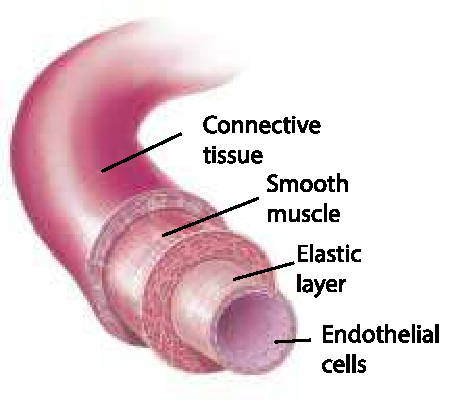
\includegraphics[width=5cm]{figure1a}
		\caption{Layers of the arteries}
		\label{fig:arteries composion}
	\end{subfigure}%
	~ 
	\begin{subfigure}[t]{0.33\textwidth}
		\centering
		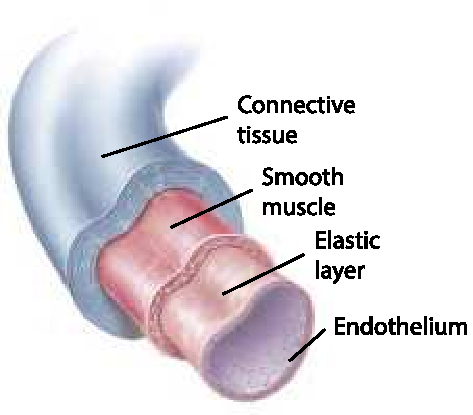
\includegraphics[width=5cm]{figure1c}
		\caption{Layers of the venous}
		\label{fig:veins composition}
	\end{subfigure}
	~ 
	\begin{subfigure}[t]{0.33\textwidth}
		\centering
		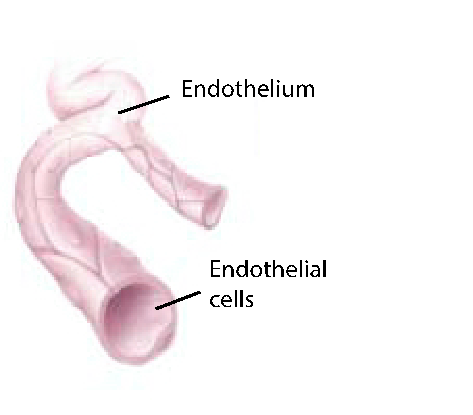
\includegraphics[width=5cm, trim={0 0 2cm 0},clip]{figure1b}
		\caption{Layers of the capillaries}
		\label{fig:capillaries composition}
	\end{subfigure}
	\caption[Layers of the blood vessels]{The arteries and veins have the same kind of layers. However, the smooth muscle is thicker in arteries than veins. The capillaries have a thin wall and are composed only by endothelium. Figure adapted from \cite{johnson2001biology}.}
	\label{fig:vessels composition}
\end{figure*}

\subsubsection{Arteries and arterioles}
The arteries slightly differ from the arterioles in their composition. The main arteries contain additional elastic fibres within them, enabling greater compliance while receiving blood coming out the heart. On the other hand, smaller arteries and arterioles contain thicker smooth muscle layer in their tunica media allow them to resist bursting.  

There is a direct relation between the diameter of the vessel and the frictional resistance to blood flow. The resistance to blood flow is inversely proportional to the radius of the vessel. Halving the diameter of a blood vessel increases 16 times its frictional resistance. Hence, the greatest resistance to blood flow in this branch of the circulatory system occurs in the small arteries and arterioles. Moreover, when the smooth muscle layer of the arterioles contracts, it produces vasoconstriction, which increases resistance and decreases blood flow. On the other hand, when this muscle relaxes vasodilation occurs, dropping resistance and increasing blood flow. Local chemical factors, the sympathetic system or hormones can control both muscle activities. Furthermore, blood flow towards some organs can also be regulated by precapillary sphincters. These rings of smooth muscle can shut down capillary beds totally. For instance, in cold weather, these precapillary sphincters may close to contribute to the vasoconstriction limiting heat loss.  

\subsubsection{Capillaries}
As it was described before, the capillaries are considerable smaller than the rest of the blood vessels. In average, every one of them is about \SI{1}{\milli\meter} long and \SI{8}{\micro\meter} diameter, just big enough to allow a single RBC (\SIrange{6}{8}{\micro\meter}) pass through. The capillary tree is so dense and extensive that every cell in the human body is within \SI{100}{\micro\meter} of reach.  Due to the enormous amount of them and their intricate network,  they have the greatest cross-section area of any other kind of blood vessel. Therefore, the blood decreases its velocity allowing more time to exchange metabolites with the surrounding extracellular fluid. As soon as the blood has left the capillary, all the exchange of $O_2$, nutrients, $CO_2$ and waste products have taken place. 

It must be noted, that the heart must produce enough pressure to overcome the resistance of the blood passing the arterial tree into the capillaries. However, blood loses most of its pressure when moving through the capillary network but also passes to a low-pressure system when entering to the veins. 

\subsubsection{Venules and veins}
Venules collect the blood that leaves the capillaries and then is deposited in the larger veins that lead the blood back to the heart. Because the pressure in the venous return is one-tenth of the arteries, venules and veins contain a thinner layer of smooth muscle. This pressure gradient also helps the blood to pass through the narrow passages of the capillaries. Most of the blood volume is contained within the veins, which also have the ability to expand to increase the body's blood capacity if needed. In order to help the blood return from the extremities, the surrounding skeletal muscle contracts by compressing the veins pushing the blood back to the heart. Also, the veins contain valves that only allow blood to flow in one direction. However, sometimes these valves may fail to lead to a vascular problem such as varicose veins. 

\begin{figure}[!htpb]
	\centering
	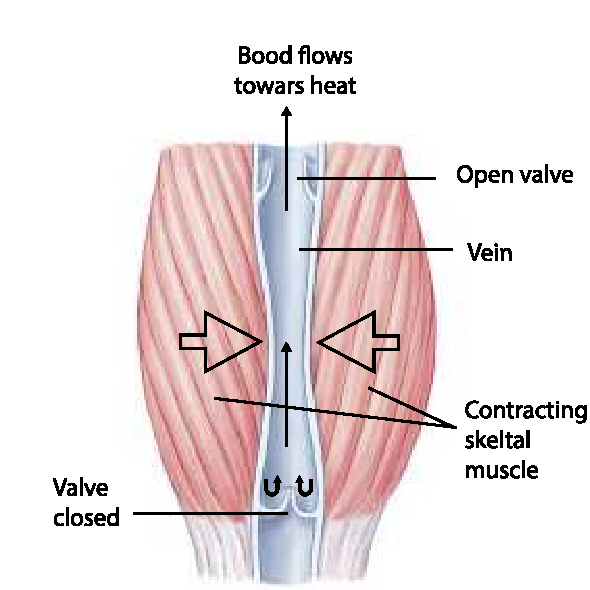
\includegraphics[width=0.5\textwidth,keepaspectratio]{figure2}    
	\caption[Venous return through skeletal muscle]{The vein only flows in on direction helped by valves along the vessel. Skeletal muscle contraction aids the return of blood to the heart. Figure adapted from \cite{johnson2001biology}. }
	\label{fig:venous return}
\end{figure}

\section{Cardiac cycle}
It is important to understand how the heart operates because changes of volume are synchronous to the heart beating. As part of the circulatory cycle, the heart has to overcome the pressure of pushing RBC's through the capillaries. Hence, the heart has to go work as a dual pump, pushing out arterial and collecting venous blood. The cardiac cycle is a periodic task that starts at the beginning of one heart beat until the start of the following one. The cycle is divided into ventricular contraction known as systole and ventricular relaxation called diastole. 

Each cardiac cycle is subdivided into phases where the heart experiences intense pressure change at constant volume or a volume change with a minor alteration in pressure. During the systolic cycle the heart experiences isovolumic contraction followed by blood ejection. On the other hand, diastole cycle follows the next steps isovolumic relaxation, rapid ventricular filling, slow ventricular filling (diastasis) and atrial contraction. The heart rate is inversely proportional to the cardiac cycle and changes according to the body's needs. An average heart rate is about 75 beats per minute, where a single beat last around \SI{0.8}{\second}.

At resting, the duration of the systolic cycle takes about 1/3 of the total heart cycle and the diastolic cycle 2/3. At high heart rate during exercise, this rate proportion changes, the duration of diastole takes much less time than the systole one. The following sections will describe the changes on the heart, as well as pressures, electrical activity and heart sounds all along each cycle.

\subsection{Systole}
\subsubsection{Isovolumic contraction}
As his name suggests iso (greek equal) volumic (volume) contraction, in this stage the heart keeps the same blood volume while the ventricles contract.
\mynote{I have to double check the ethimology of this word}

Figure \ref{fig:heart isovolumic} shows the cross-section of the heart during this stage of the systole. In this part, depolarization of the ventricle causes ventricular contraction which swiftly increases the pressure inside both ventricles. Right after the ventricular contraction occurs, due to a higher pressure in the ventricle than in the atria then the atrioventricular valves close. Moreover, the semilunar valves are also shut due to ventricular pressure is lower than the one in the arteries (aorta and pulmonary).

\begin{figure}[!htpb]
	\centering
	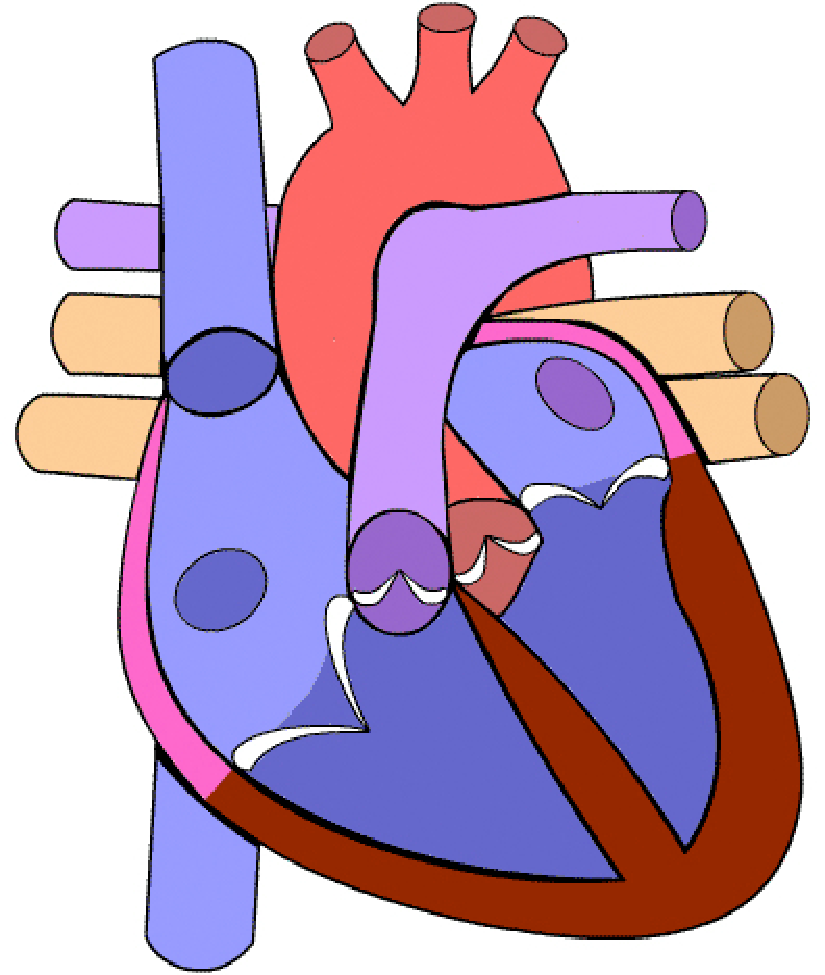
\includegraphics[width=0.25\textwidth,keepaspectratio]{figure_3}    
	\caption[Isovolumic contraction]{Cross section of the heart during isovolumic contraction. The contracted area is represented by the red colour.}
	\label{fig:heart isovolumic}
\end{figure}
\mynote{I need to reference this to the website}

Figure \ref{fig:pressure isovolumic} shows the variation of pressure in the left ventricle, the right atrium, the aortic pressure and the ventricular volume. As the valves are shut and the ventricles are contracted and blood can not leave the heart, thus the ventricular pressure increases but there is no a changes in the blood's volume. In the end, the total volume inside the ventricles is equivalent to the end-diastolic volume (about \SI{130}{\milli\liter}. In the atria, due to the differential of pressure between chambers the atrioventricular bulges backwards. Therefore, this valve change causes a small variation of pressure in the right atrium. It is depicted as the point c in the figure same figure. The pressure in the systemic and pulmonary arteries drops at a constant rate. 

\begin{figure}[!htpb]
	\centering
	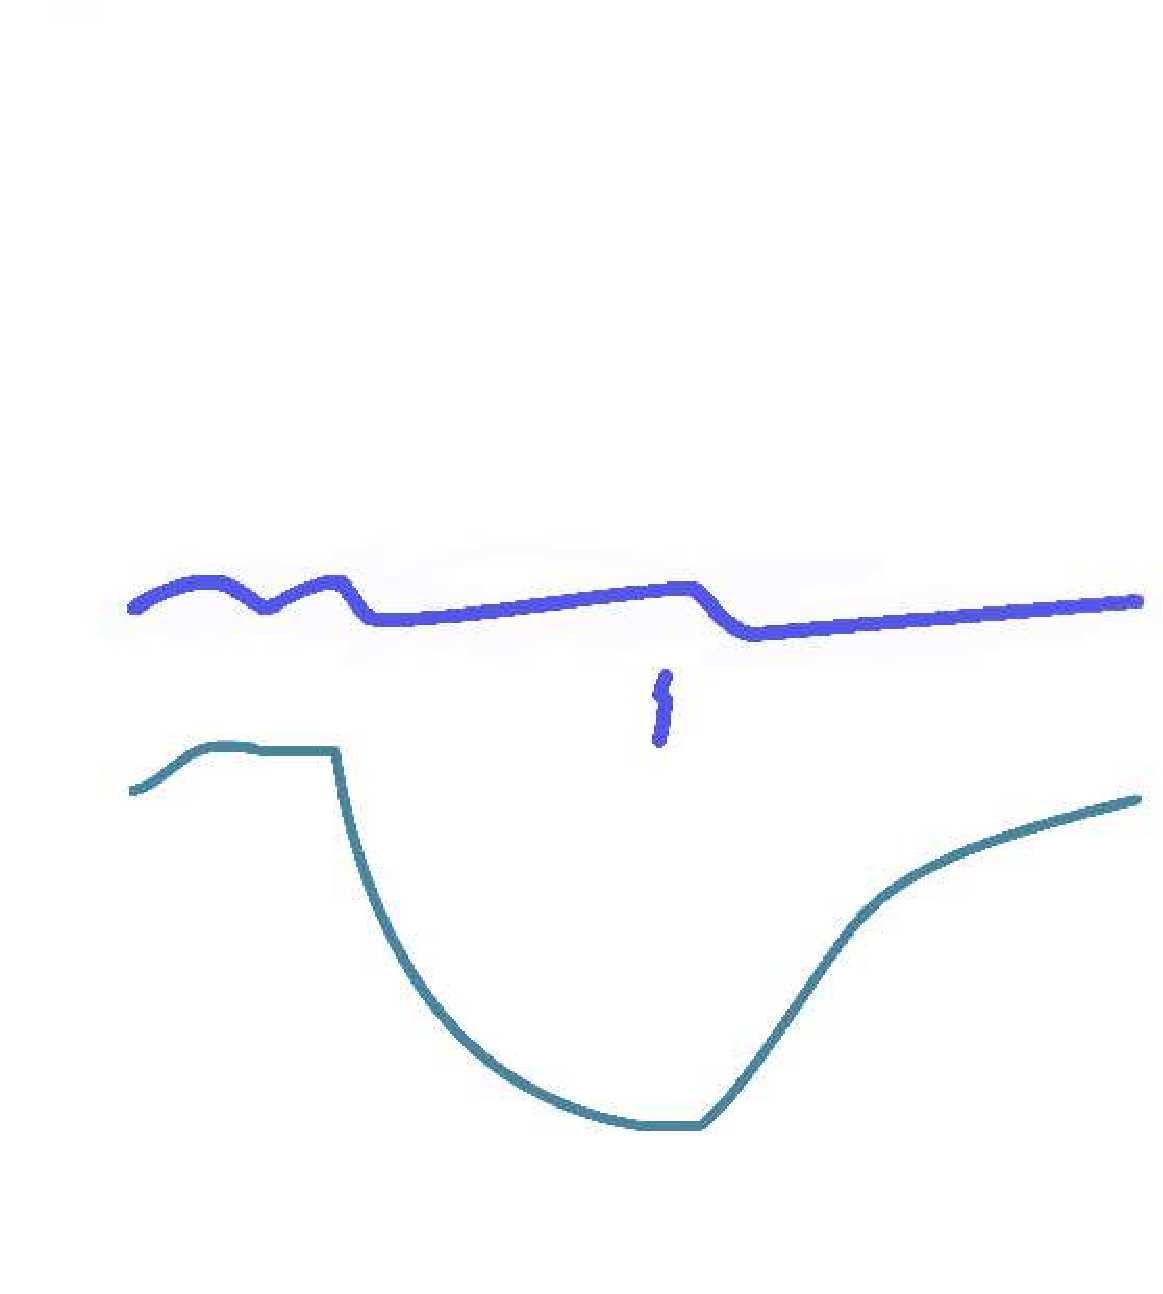
\includegraphics[width=0.5\textwidth,keepaspectratio]{figure_4}    
	\caption[Isovolumic contraction - pressure and volume changes]{Pressures and volume changes during isovolumic contraction in the highlighted area. In red the pressure of the left ventricle, in black the aortic pressure, dark blue the pressure of the right atrium and light blue the ventricular volume.}
	\label{fig:pressure isovolumic}
\end{figure}
\mynote{I need to reference this to the website.}
\mynote{If I have time, I should get this data and create my own plot.}

The electrocardiogram waveform shown in figure \ref{fig:ECG isovolumic} displays the electrical activity of the heart during this section of the cycle. In short, the depolarization of the heart starts from the atrioventricular node spreading through the bundle of His and Punkyne fibres to the septum and the walls of both ventricles. This event causes the QRS complex shown in the same figure. At the same time, the atria repolarisation causes the atrial T wave which is not visible in the ECG because QRS complex covers it.

\begin{figure}[!htpb]
	\centering
	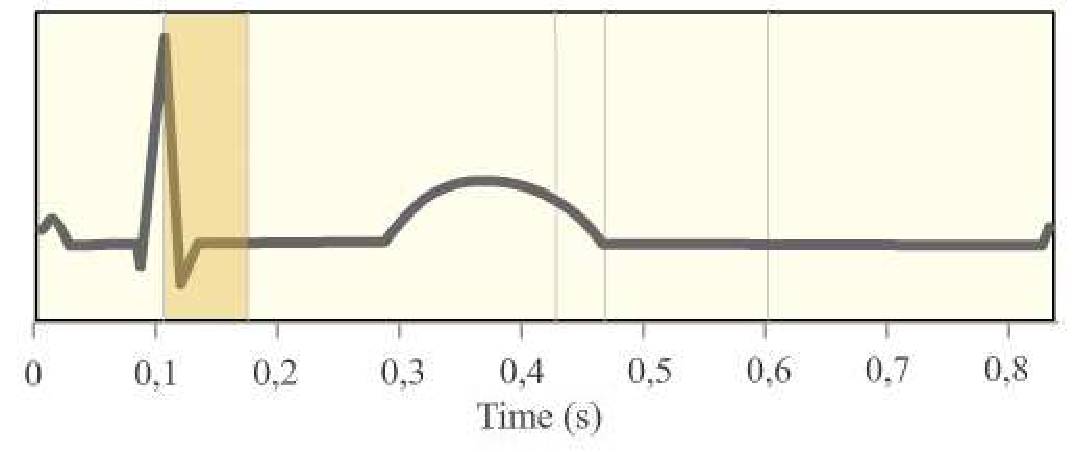
\includegraphics[width=0.5\textwidth,keepaspectratio]{figure_5}    
	\caption[Isovolumic contraction - ECG]{ECG during isovolumic contraction.}
	\label{fig:ECG isovolumic}
\end{figure}

During this stage the first sounds of the heart are perceptible with echocardiography. 
 
\section{Upper limb anatomy}

%********************************** %Section 2.1.2  **************************************
\section{Oxygen transportation}
\label{section literature 1.2}
Oxygen ($O_2$) is an essential component needed by all body's cells to complete metabolic processes. Within the blood, this is transported by haemoglobin (Hb) contained within red blood cells (RBCs). Oxygen is required for the chemical reactions needed to convert biochemical energy from nutrients coming from food into cell's energy known as coenzyme or adenosine triphosphate (ATP). As a result of this reaction waste product is released from the cell. A human cell can only survive for a few minutes without oxygen~\cite{culmsee2005apoptosis}.

Inadequate oxygen delivery to body's tissue is known as hypoxia. There are different classifications of hypoxia count based on its cause~\cite{marieb2007human} which are described as follows: 

\begin{enumerate}
    \item \textbf{Anaemic Hypoxia:} It is a condition where a body part or an organ has poor $O_2$ delivery. Some of the causes are a small count of RBCs and abnormal or too little Hb content in the blood's cells.
    \item \textbf{Ischemic (stagnant) hypoxia: }This is caused when blood circulation is reduced or blocked. There are different causes for this. However, the most commons are congestive heart failure that may cause body–wide hypoxia, emboli or thrombi blocking oxygen supply to the tissue distal from the occlusion. 
    \item \textbf{Histotoxic hypoxia: }Mainly caused by metabolic poisoning like ingestion of cyanide. In this case the cell is unable to use $O_2$ for metabolic purposes, even though there is an appropriate amount of $O_2$ being delivered by the body.
    \item \textbf{Hypoxemic hypoxia:} It is shown by a decrease in the arterial oxygen partial pressure ($PO_2$). Some of the causes are an imbalance in the ventilation–perfusion coupling mechanism, poor ventilation caused by pulmonary disease and breathing air with a low content of $O_2$. Moreover, carbon monoxide ($CO$) poisoning is another reason behind this illness because it has \num{200} times more affinity with Hb than $O_2$. Thus, in places with high concentration of CO such as fires could lead easily to death.
\end{enumerate}




%********************************** %Section 2.2  **************************************
\subsection{Problems derived from poor blood delivery} %Section 2.3
\label{section literature 3}
Now that has been described some of the problems of having a poor oxygen transportation of blood at a cellular level; more detail will be unveiled about illnesses due to the poor or total lack of blood delivery to human tissue especially human limbs. 

Ischemia develops when there is an insufficient supply of blood to an organ. For instance, if an artery blockage occurs all the tissue below the path will suffer from starvation of oxygen and other critical nutrients. Different causes could lead to the blockage of an artery which can be caused by external or internal factors. Speaking specifically of lower limbs, these represent a significant cause of disability and cardiovascular morbidity and mortality~\cite{novo1995patients}. 

Exists different kind of diseases compromising limbs, an example of this is peripheral arterial disease (PAD), which also originates in another kind of illnesses according to the kind of occlusion or blockage. For instance, critical limb ischemia (CLI), which is a condition where as a consequence of arterial disease, a patient experiments pain in the extremity even at rest or in a breakdown of the skin~\cite{novo2004critical}. 

Clinically there are different forms to assess the development of this illness. Some scales of qualitative evaluation have been developed such as the Rutherford classification, the Leriche-Fountaine classification or the TACS II classification of femoral and popliteal lesions~\cite{norgren2007inter}. Health practitioner uses a survey, an indicator of pain when walking and a visual inspection is possible to determine the stage or the severity of the arterial occlusion.  Table \ref{table:Fountaine}) shows the different stages of the Leriche-Fountain classification and the various steps considered to evaluate the illness.

\begin{table}
\caption{Leriche-Fountaine classification}
\centering
\label{table:Fountaine}
\begin{tabular}{p{1.8cm} p{3.8cm} p{3.5cm} p{4.5cm}}
\toprule
\textbf{Stages}& \textbf{Symptoms} & \textbf{Pathophysiology} & \textbf{Pathophysiological \newline classification} \\
\midrule
Stage I & Asymptomatic \newline or effort pain & Relative hypoxia & Silent Arteriopathy \\
\midrule
Stage II A & Effort pain \newline Pain free walking distance > \SI{200}{\meter} & Relative hypoxia & Stabilized Arteriopathy \newline Non-Invalidant claudication \\ 
\midrule
Stage III A & Rest Pain \newline Ankle arterial pressure > \SI{50}{\mmHg} & Cutaneous hypoxia \newline Tissue acidosis \newline Ischemic neuritis & Instable arteriopathy \newline Invalidant claudication \\
\midrule
Stage III B & Rest pain \newline Ankle arterial pressure < \SI{50}{\mmHg} & Cutaneous hypoxia \newline Tissue acidosis \newline Ischemic neuritis & Instable arteriopathy \newline
Invalidant claudication \\
\midrule
Stage IV & Trophic lesions \newline Necrosis or Gangrene & Cutaneous hypoxia \newline 
Tissue acidosis & Necrosis \newline Evolutive arteriopathy \\
\bottomrule
\end{tabular}
\end{table}

As table~\ref{table:Fountaine} shows, there are various levels of stratifying the severity of the disease according to the symptoms that are related pathophysiology. According to the gravity of the stage where the patient is, there are different methods to examine the severity of the disease using imaging methods. These will be described in detail in the section xxx.

\mynote{relate this to a section in the document later on}

There are a significant number of illnesses that are derived from the inadequate delivery of blood towards a limb. According to their physiology, they can be divided into a disease which affects either the microcirculation or main vessels or both. The following are just an example of the different diseases that may require continuous blood flow monitoring in acute or chronic settings.



%********************************** %Section 2.2.1  **************************************
\subsubsection{Peripheral vascular disease}
\label{section literature 2.1}
Some of the common forms of reduction in blood towards a limb are known as the peripheral vascular disease (PVD) also known as peripheral arterial disease (PAD). This sickness is a progressive vascular condition caused by the blockage, narrowing, or spasms in a blood vessel (arteries, veins or lymphatic vessels). Hence, altering the blood circulation to and from any upper or lower extremities.  Most commonly affect the lower limbs, especially legs and feet. Therefore, the derivation of its name as "peripheral" because it affects mostly the periphery of the body. It affects \SI{5}{\percent} of people over \num{50} and between \SIrange{12}{20}{\percent} of people over 65 years old. To some extent, it is more common in men than women. People with certain risk factors are more likely to suffer PVD such as patients with diabetes of smokers.  

\mynote{I need a reference for this numbers}

Different factors could cause the narrowing of the blood vessels. The most common cause of PVD is atherosclerosis, deposition of fatty material on the arterial walls. This fatty material constitutes a plaque that reduces the blood flow towards tissue in the limb lessen the transport of $O_2$ and nutrients as explained in Oxygen transportation section. Moreover, clots may also form on the artery walls reducing the internal size of the vessel and increasing the risk of obstructing off a major artery. 

Different risk factors are contributing to the development of this sickness. Some can be inherited to the population others are based on lifestyle choices. The combination of two of more of the following risks may increase complications from PVD, such as smoking and diabetes. However, more in details some of the documented risk factors are:

\begin{itemize}[noitemsep]
    \item Age (especially over \num{50})
    \item Family history (high blood pressure, high cholesterol or PVD)
    \item Diabetes
    \item Smoking
    \item Obesity
    \item Infections
    \item Coronary artery disease
    \item Injury to vessels
    \item Physical inactivity
    \item High blood pressure
    \item Autoimmune diseases
    \item Nutritional deficiencies
    \item High blood cholesterol
    \item Emboli from other locations in the body
    \item Inflammation of the blood vessels
\end{itemize}

On the first stages of the illness, symptoms are not noticeable, which makes difficult to diagnose the condition. Just until it has been developed into a painful stage as described by the Fountaine's classification (see table \ref{table:Fountaine}) is when actions come into place. However, performing a qualitative assessment of the extremity helps to diagnose the sickness in early stages. Some of the indicators could be coldness to touch, poor skin condition (thinning, shining or brittle), poor nail health (thickening or opaque nails), hair loss in the extremity, reduced pulse sensation in the extremity, impotence, infections or injuries not healing properly, poor muscle condition (numbness, weakness or heaviness), pain while walking and stop at rest, local skin discolouration (pale, blue or dark red) and restricted mobility. 

Once a qualitative or physical examination has been performed, and the progress of the illness has been classified there are additional tests that may help to diagnose the severity of the PVD. Some of the methods just require the assessment of the medical practitioner using common medical devices others may need the use of specialised equipment. Some of the therapeutic methods that do not demand the use of bulky or cumbersome devices are:

\begin{itemize}
    \item \textbf{Ankle-branchial index (ABI):} It is the ratio of the differential measurement of systolic blood pressure measured at the ankle to that measured at the brachial artery [17]. For this it is required to compared the difference in blood pressure between the arm and the ankle, it also needed to record the ankle's blood flow using a Doppler ultrasound instrument.  
    \item \textbf{Treadmill exercise test: }In this method the patient has to walk or run to monitor the circulation during exercise. Pain or problems during the test are recorded to examine the severity of the obstruction.
    \item \textbf{Reactive hyperaemia test:} This test refers to a temporary increase (\textit{hyper}) of blood flow (\textit{emia}) of the extremity. It is usually performed in people who are not able to walk on a treadmill. In this case, the person is taken to supine position and comparative measurements of blood flow in tights and ankles are taken after occlusion to determine any decrease between both sites. 
\end{itemize}

%********************************** %Section 2.2.2  **************************************
\subsubsection{Compartment syndrome}
\label{section literature 2.2}                                                                                                                                                                                                                                                                                                                                                                                                                                                                                                                                                                                                                     
All the muscles, blood vessels and nerves are contained within a tissue known as fascia. When the pressure in a limb within this compartments increases because of bleeding or swelling, it could lead to total or partial restriction of micro–vascular blood flow \cite{songer2001tissue}. Some cases may present rapid discolouration and blistering of the affected limb being commonly associated with oedema, cyanosis and severe pain \cite{chhabra2013compartment}. Hence, it can lead ultimately to venous hypertension and loss of blood plasma. If the arterial flow is reduced, it also may result in gangrene, limb loss or even death \cite{lamborn2014compartment}. This syndrome can be catalogued as acute when is caused by either an injury, accident or medical emergency, and chronic when occurs gradually during any sports activity.

The most common method to diagnose this illness is Doppler sonography \cite{chhabra2013compartment}. Nevertheless, detecting foot compartment syndrome could be challenging compared to other parts of the body because its symptoms and indicators are less reliable \cite{dodd2013foot}.

%********************************** %Section 2.2.3  **************************************
\subsubsection{Diabetic foot infection}
\label{section literature 2.3} 
The lack of blood towards an extremity can also be caused by a secondary effect of other illness like diabetes. Some of the most common problems that diabetic patients have to deal with are diabetic foot infection which is a clinical syndrome characterised by local findings of inflammation or purulence in a person with diabetes. Also, it also leads to a decrease in peripheral circulation, vascular disease and loss of nerve sensation ending up in the formation chronic ischemic ulcers and bacterial infection. Diabetes is the leading cause of lower extremity amputation in developed countries, and it is responsible for \SI{60}{\percent} of these amputations~\cite{ucckay2014diabetic}.  Currently, Doppler ultrasound flowmetry is still one of the primary tools to diagnose the advance of Diabetes foot infection (DFI). Although, new techniques to follow up the progress of this illness have been researched such as bioelectrical impedance~\cite{cheng2012application}, planar pressure analysis~\cite{dos2010insole}, imagine technique analysis~\cite{songer2001tissue}, near infrared~\cite{papazoglou2008assessment} and electronic noses~\cite{yusuf2013diagnosis}. Until now, nothing has been designed to detect early stages of this problem before ulceration occurs. Regarding bioelectrical impedance analysis (BIA), there have been studies focused on the detection on the development of ischemia of the foot's sole showing a good correlation with laser Doppler flowmetry~\cite{cheng2012application}. 

\section{Plethysmography}
\label{section literature 3}
The word plethysmography roots from the Greek word \textit{plethymos} that means either increasing or enlarging and \textit{graphos} that is to write. In other words, it can be defined as the measurement of volume in the human body. In medicine, some of the common applications are the measurement of volume changes in lungs caused by the respiratory system or blood vessels caused by the circulatory system~\cite{turcott2004methods}.  More specifically when referring to the latter, plethysmography aims to measures the pulsatile volume changes when the heart pumps blood in and out in a segment of the human body. 


A plethysmography device produces an output waveform that is synchronous to the heart cycle. The shape of the signal is similar to an arterial pressure waveform. In fact, the plethysmography plot represents the volume of the arterial vasculature obtaining a measure of the arterial pulse amplitude. This waveform gives meaningful information about the pulse velocity and indications of possible arterial obstruction.

\begin{figure}[!htpb]
	\centering
	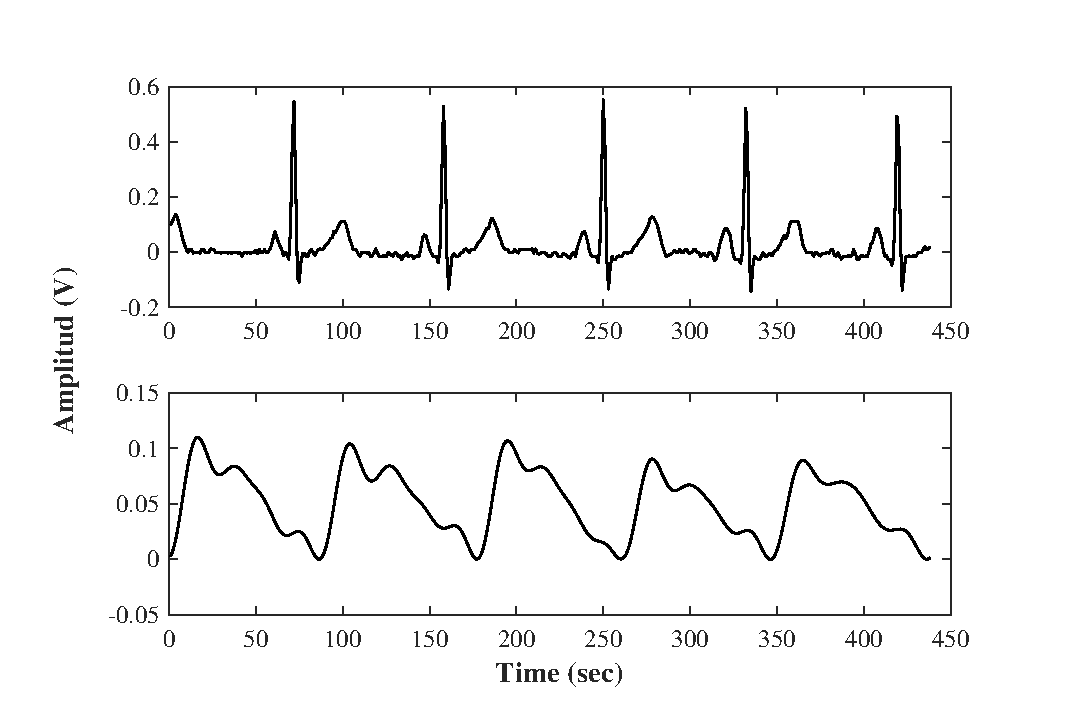
\includegraphics[width=0.75\textwidth,keepaspectratio]{figure3}    
	\caption[Classic plethysmography waveform]{Representation of a classic plethysmography waveform from the heart cycle. The image on the top represents the electrical signal of the heart (ECG). The one below is the plethysmography waveform of the circulation. Both signal are synchronous}
	\label{fig:plethysmography}
\end{figure}

There are different methods and technologies to measure plethysmography. Every method can be applied separately or as part of a system. Some techniques can measure plethysmography of the whole body, segments or localised areas. For instance, chambers of air or water are used to measure lung capacity. This chamber measures the air displacement of a patient while this inhales inside the chamber. 

For measurement of changes of volume of a limb's segment, the air plethysmography technique could be very cumbersome and not very practical. This is one of the many reasons why more techniques have been developed. The following section describes methods to detect plethysmography from a part of the body.

\subsection{Air plethysmography}
\label{section literature 3.1}
Air plethysmography is not a common method to measure a limb’s change of volume. It has been used as an either alternative or research method as explained by Chuah et al.~\cite{chuah2004plethysmography} for measurement of plethysmography without venous occlusion. This approach uses a special chamber that contains the limb in a close area with orifices where transducers and calibration devices are connected. The arm is introduced into the case through a tight rubber sleeve to ensure that the instrument is airtight.  The plethysmography pulsations are detected by measuring the displacement of the surrounding air with a sensor connected to the chamber, which also moves the rubber diaphragm which a Doppler ultrasound transducer measures displacement. As can be noticed, this method could be burdensome, and it is not very desirable to be applied during critical application such as surgery.

\begin{figure}[!htpb]
	\centering
	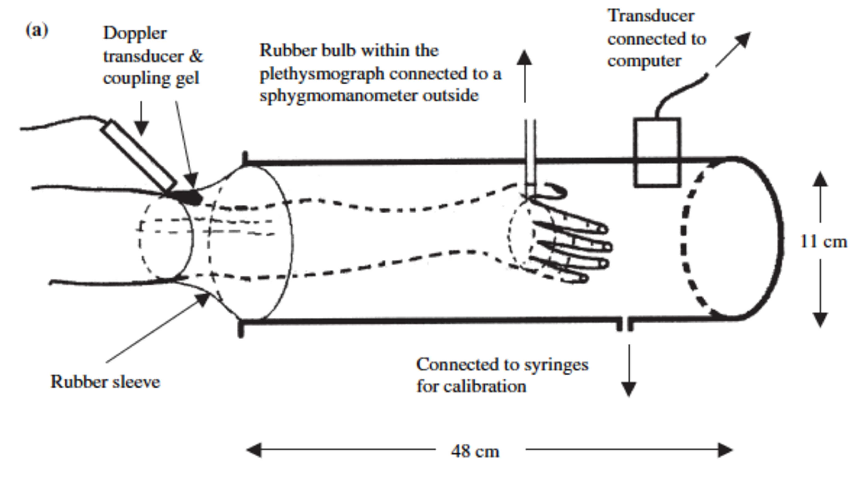
\includegraphics[width=0.95\textwidth,keepaspectratio]{figure4}    
	\caption[Air plethysmography method]{Representation of an air plethysmography device. It requires a one side open cylinder with with a rubber sleeve. There is a compartment where the air displacement caused by each cardiac cycle can be measured.}
	\label{fig:air plethysmography}
\end{figure}

\subsection{Doppler method}
\label{section literature 3.2}
The Doppler technique is not directly a plethysmography method because it does not measure changes in volume but variations of flow. In physics, both parameters are related if the cross-section area of the volume being measured is known. Hence, if the flow and area are known is possible to deduce the volume flow rate. This method uses the Doppler effect to measure blood flow non-invasively from the skin surface. It is very popular in the medical ambit. It could be implemented via ultrasound (ultrasound Doppler flowmetry) frequency or photoelectric effect (laser Doppler flowmetry).  This method measures the velocity of particles in solution using frequency shift of backscattered ultrasound or light~\cite{orekhova2013doppler} (see Figure \ref{fig:Doppler method}). 

A signal is generated to a target tissue and then reflected by the macroscopic tissue structures. Some of the energy in light or sound form is reflected, absorbed and scattered by the tissue and blood particles. This method measures the microcirculation underlying the flow of the arterioles and venules. However, this technique is mainly for superficial measurements or invasively for free flap flow measurements. For instance, it has been studied that laser Doppler flowmetry has \SI{1}{\milli\meter} of penetration. In the case of ultrasound Doppler measurements are affected by the angle of the frequency applied to the target tissue.

\mynote{reference to this depth}

\begin{figure}[!htpb]
	\centering
	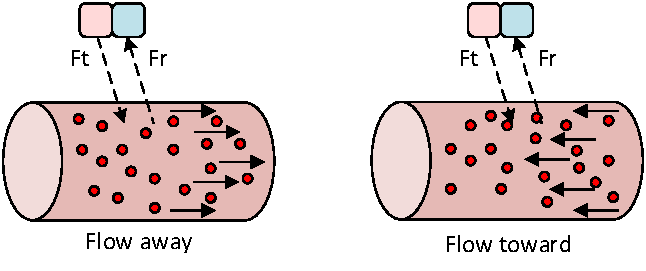
\includegraphics[width=0.75\textwidth,keepaspectratio]{figure5}    
	\caption[Doppler technique to measure flow]{Representation of a classic plethysmography waveform from the heart cycle. The image on the top represents the electrical signal of the heart. The one before is the plethysmography waveform of the circulation.}
	\label{fig:Doppler method}
\end{figure}


\subsection{Strain gauge plethysmography}
\label{section literature 3.3}
This method also known as SGP (strain gauge plethysmography) is a non-invasive method to quantify retrograde outflow in the deep venous system and peripheral arterial disease~\cite{holohan1996plethysmography}. It works by applying a strain gauge around the limb under test. The transducer could be a tube filled in with a conductive material such as mercury and gallium and connected to a source of electricity. However, alternative methods that do not use clinically banned mercury have been developed using electrical conductive fluids~\cite{flowers1981strain}. When the gauge experiences variations of circumference caused by a change of volume of the rib cage or the pulse in a limb, the resistance of the sensor also vary accordingly obtaining an electrical waveform. To increase sensitivity for venous filling measurements occlusion cuffs would be required, as shown in Figure~\ref{fig:strain gauge}. This method does not provide reliable quantitative data for venous occlusion but provides qualitative data for the function of the extremity in venous insufficiency~\cite{holohan1996plethysmography}. 

\begin{figure}[!htpb]
	\centering
	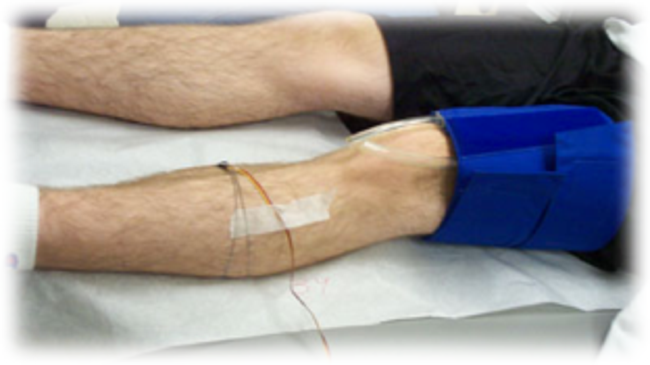
\includegraphics[width=0.75\textwidth,keepaspectratio,trim={0.5cm 0.5cm 0.5cm 0.5cm}, clip]{figure6}    
	\caption[Strain gauge plethysmography]{Representation of a classic plethysmography waveform from the heart cycle. The image on the top represents the electrical signal of the heart. The one before is the plethysmography waveform of the circulation.}
	\label{fig:strain gauge}
\end{figure}


\subsection{Photoelectric method}
\label{section literature 3.4}
This method is technically known as photoelectric plethysmography or PPG for short. It is one of the most popular methods used in medical applications nowadays. It is a non-invasive method that uses different light wavelengths to obtain a plethysmography graph. It is widely used for monitoring or evaluating heart rate, oxygen saturation, peripheral arterial pressure and peripheral microcirculation after skin grafting, drug ingestion, burns or revascularization~\cite{holohan1996plethysmography}. There are two different techniques to obtain readings. One is transmission-mode (see figure \ref{fig:PPG transmission}.) that works by placing the tissue of interest (i.e. finger, toe or ear lobe) between the light emitting diode (LED) and the photoreceptor (PD).  The other is PPG reflectance-mode (see figure\ref{fig:PPG reflectance}) by placing the LED next to photoelectric cell over the surface of the tissue o study. PPG uses the AC component of the signal for arterial pulse detection and the DC component for venous evaluation~\cite{higgins1986photoplethysmographic}. It also uses a different kind of wavelengths to avoid interference from external sources of light. The principle behind PPG is the detection of the degree of attenuation of backscatter light from the superficial layers of skin about \SIrange{1.5}{2.0}{\milli\meter} ~\cite{holohan1996plethysmography,kim1986pulse}. The amount of reflected light varies with the total number of RBC’s in the cutaneous microcirculation, which alters the wavelength during each cardiac cycle. This method has been proved to be effective for the initial diagnostics of peripheral arterial disease (PAD) and chronic peripheral venous insufficiency (CVI).

Some of the disadvantages of PPG are that only measures a small area at the time. Therefore, it is not possible to get a spatial distribution of the blood volume change over the skin~\cite{wu2003ppgi}. Also, skin pigmentation has been probed being an error factor as well as nail polishers~\cite{fallow2013influence}. 

\begin{figure*}[!htbp]
	\centering
	\begin{subfigure}[t]{0.5\textwidth}
		\centering
		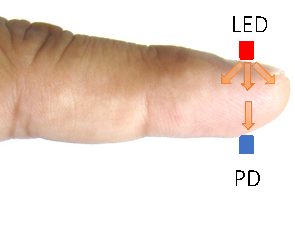
\includegraphics[height=4cm]{figure7a}
		\caption{Placement of LED and photodetector in transmission mode}
		\label{fig:PPG transmission}
	\end{subfigure}%
	~ 
	\begin{subfigure}[t]{0.5\textwidth}
		\centering
		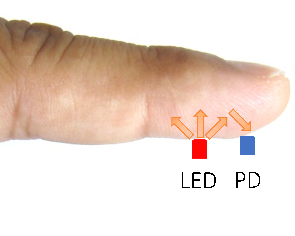
\includegraphics[height=4cm]{figure7b}
		\caption{Placement of LED and photodetector in reflectance mode}
		\label{fig:PPG reflectance}
	\end{subfigure}
	\caption[PPG sensors placemens as transmission and reflectance modes]{PPG light emitter placement and receptor according to the mode, transmission and reflectance}
	\label{fig:PPG modes}
\end{figure*}

\subsection{Bioelectrical Impedance}
\label{section literature 3.5}
Also known as impedance plethysmography (iPG) involves the measurement of the change in impedance due to change of blood flow. For instance, when heart’s systole increases blood flow, the volume of a limb rises due to the inflow of blood (swelling)~\cite{martinsen2011bioimpedance}. Consequently, there are changes of impedance correlated to the changes of volume and flow in a limb. Some medical application might require the use of occlusion cuffs to analyse venous filling. There are several medical applications for this kind of technique such as heart stroke volume (SV) measurement, cardiac output (CO), thoracic respiratory volume, oedema and detection of deep vein thrombosis (DVT)~\cite{holohan1996plethysmography}.

The following section describes more in detail the definition of iPG, how it works, medical applications, how is measured and the possible ways to represent it. This information will help to understand how volume and ischemia can be related to calculating an index between the two measurements.

%********************************** %Nomenclatures in chapter  **************************************
\nomenclature[z-Hb]{Hb}{Haemoglobin}
\nomenclature[z-ATP]{ATP}{Adenosine Triphosphate}
\nomenclature[z-rbc]{RBC}{Red Blood Cells}
\nomenclature[z-abi]{ABI}{Ankle-Branchial index}
\nomenclature[z-wbc]{WBC}{White Blood Cells}
\nomenclature[z-PVD]{PVD}{Peripheral vascular disease}
\nomenclature[z-bia]{BIA}{Bioelectrical impedance analysis}
\nomenclature[z-DFI]{DFI}{Doppler flowmetry}
\nomenclature[z-DVT]{DVT}{Deep vein thrombosis}
\nomenclature[z-cli]{CLI}{Critical Limb Ischemia}
\nomenclature[z-PAD]{PAD}{Peripheral Arterial Disease}
\nomenclature[z-SV]{SV}{Strove Volume}
\nomenclature[z-LED]{LED}{Light emitting diode}
\nomenclature[z-CVI]{CVI}{Chronic peripheral venous insufficiency}
\nomenclature[z-ppg]{PPG}{Photoplethysmography}
\nomenclature[z-ipg]{iPG}{Impedance Plethysmography}
\nomenclature[z-CO]{CO}{Cardiac output}
\nomenclature[z-SGP]{SGP}{strain gauge plethysmography}
\nomenclature[z-BIA]{BIA}{Bioelectrical impedance analysis}


%\nomenclature[z-cif]{$CIF$}{Cauchy's Integral Formula}                                % first letter Z is for Acronyms 
%\nomenclature[a-F]{$F$}{complex function}                                                   % first letter A is for Roman symbols
%\nomenclature[g-p]{$\pi$}{ $\simeq 3.14\ldots$}                                             % first letter G is for Greek Symbols
%\nomenclature[g-i]{$\iota$}{unit imaginary number $\sqrt{-1}$}                      % first letter G is for Greek Symbols
%\nomenclature[g-g]{$\gamma$}{a simply closed curve on a complex plane}  % first letter G is for Greek Symbols
%\nomenclature[x-i]{$\oint_\gamma$}{integration around a curve $\gamma$} % first letter X is for Other Symbols
%\nomenclature[r-j]{$j$}{superscript index}                                                       % first letter R is for superscripts
%\nomenclature[s-0]{$0$}{subscript index}                                                        % first letter S is for subscriptsd

%!TEX root = ../thesis.tex
%*******************************************************************************
%****************************** Second Chapter *********************************
%*******************************************************************************

\chapter{Design of impedance plethysmography device}

\ifpdf
    \graphicspath{{Chapter3/Figs/Raster/}{Chapter3/Figs/PDF/}{Chapter3/Figs/}}
\else
    \graphicspath{{Chapter3/Figs/Vector/}{Chapter3/Figs/}}
\fi


%********************************** %First Section  **************************************
It is well known that detecting changes of volume in the human body, provides valuable medical information. Ischemia is known as lack of blood supply towards an organ or tissue. Most common cases occur when there is a blockage in an artery. Thus, leading to tissue starvation because of lack of oxygen and nutrients. One of the most common diseases that involves extremities is the peripheral arterial disease. This is a progressive vascular illness caused by blockage, narrowing or spasms in blood vessels such as arteries, veins or lymphatic vessels. Referring to limbs, these represent an important cause of disability and mortality~\cite{novo1995patients}. Knowing patient's haemodynamic conditions may help medical therapists to follow an appropriate plan of treatment according to the severity of the condition.

Electrical impedance plethysmography is a method non-invasive, portable, comfortable, safe, unperceivable, simple and easy to implement.  It can detect changes of blood volume not just in the periphery but also other parts of the body. In short, this method takes advantage of blood and tissue conductive properties. It has a resistive response when an alternating current is applied. Ionic conduction of a segment of the body reflects the same behaviour of electric conduction in metallic cylinders. Since 1950's, it has been extensively proved that changes in arteriovenous blood volume in an extremity segment is directly related to static and dynamic changes of impedance measurements in synchrony with the heart cycle.

The genesis of impedance plethysmography can be traced back to the model proposed by Jan Nyober~\cite{nyober1959electrical}. The author describes extremities as cylinders. The total electrical conductance path is resulting from the sum of the parallel conductance of blood and tissue within a segment. In fact, this theory called parallel conductor was later confirmed by the experiments performed by Shimazu et al~\cite{shimazu1982evaluation}. There have been some doubts about how much is blood's impedance contribution to the total impedance signal.  It has been demonstrated through in vitro experiments that blood (haematocrit = $ 26 \pm 4 \%$) contributed to \SI{10}{\percent} of the signal. In the test, a saline buffer solution was compared between extensile arteries and rigid tubes~\cite{peura1978influence}. 

Nyober proposed that the effective parallel resistive value of the displaced blood can be originated from the parallel relation between the original base resistance and the new resistance value, given by the following expression:

\begin{align}
R_B=\frac{R_N R_0}{R_0-R_N} \approx \frac{R^2_0}{\Delta R}
\end{align}

where $R_0$ is equivalent to the original resistance and $R_N$ represents the increase of new total resistance. The denominator $R_0 - R_N$ is equivalent to $R$, peers with the change of impedance caused by blood volume expansion during the heart cycle. From this, the author deducted the following governing equation. That shows that proportional increment of blood volume uniformly distributed within a cylindrical segment can be derived from the equation of the volume of a cylindrical conductor:

\begin{align}
V_B = \rho \frac{l^2}{R_B}
\end{align}

in which  is equivalent to the resistivity of the blood, is the length of the segment which is equivalent to the distance of the measuring electrodes and the value of  that was described previously as the parallel value of resistances.

Different equations aroused complementing the Nyboer's work. One of this modification's is the Kubicek et al method~\cite{karnegis1966development}. His equation is widely used specially when measurements from the measurement of impedance cardiography from the thoracic box and to deduct stroke volume of the heart. Other, well known work is Sramek~\cite{sramek1986bomed} contribution. This is also modification of Kubicec equation where the author eliminates the dependence $l$ and $\rho$,  and introduces a data obtained from statistical methods named volume of electrical participating tissue. 

From the equations named previously different kind of haemodynamic information can be obtained. The most common used as describe before is plethysmography information based on the principle described. However, different uses have been applied to the signals obtained from impedance plethysmography. 

For instance, some measurements require changes in the basal impedance which is the base impedance for tissue, fat, skin, bone and blood when there is no expansion of volume. For better understanding this can be described as the DC content of a signal or in the case of Nyober's parallel conductor is equivalent to . This is particularly popular when used to estimate blood flow in extremities. The method that uses this kind of data is referred as venous occlusion plethysmography. In this method, a cuff is inflated \SIrange{10}{20}{\mmHg} below systolic for a period and then released. Some of its applications can be seen being applied in the work performed by Mohapatra~\cite{mohapatra1979measurement} and Schraibman~\cite{schraibman1975comparison}, where a comparison of the change of volume using strain gauge and impedance in patients under anaesthesia showed a significant relationship between both techniques.

Yamakoshi~\cite{shimazu1982evaluation,yamakoshi1980limb,yamakoshi1978admittance}  in his research and patent work also uses the same method to estimate blood flow but instead of using impedance uses its reciprocate admittance $(Y=Z^{-1})$ for easy computational results. In his work, the author states that the initial gradient of the computation result to time is indicative of the blood rate in the limb being examined.
 
The plethysmography waveform is utilized to also quantify measurements of pulsatile volume, blood flow beat to beat, blood pressure and pulse wave velocity. In this case, the waveform is like the AC component of the impedance signal. The contribution of this signal to the total of the signal is between \SIrange{0.1}{1}{\percent} of the total of the signal. Sometimes, it is necessary to implement low noise techniques to picking-up the signal hidden within the basal impedance. 

The most common application to the waveform is the quantification of blood flow beat to beat. Compared with the previous technique, this method does not require venous occlusion. By applying Nyboer's equation to the waveform signal is also possible to quantify peak-peak blood volume and peak net inflow. For instance, the patent presented by Marks~\cite{marks1985computer} shows the application of quantifying blood flow in upper extremities by computing the derivatives of the waveform signal producing the results claimed. Other example, taking measurements from lower limbs is the work performed by Porter~\cite{porter1985measurement} where an impedance cardiograph was used to obtain the waveform signals and computed using Kubicek's equation and concluding the potential use of the signal to evaluate limb oedema. 

Other application to the waveform is the valuation of blood pressure continuously. As it is explained by Blinov~\cite{blinov1997plethysmographic} pressure could be deducted if blood flow can be estimated. As it was explained before, blood flow can estimated beat-beat by deriving the waveform after applying Nyober's equation as result the equation transforms into:

\begin{align}
dV = \rho \frac{l^2}{R^2_B} dR
\end{align}

Volume rate is defined as the change of volume in time. Then blood flow rate $(\dot{Q})$ is defined by the following equation:

\begin{align}
\dot{Q} = \frac{dV}{dt}=-\rho \frac{l^2}{R^{2}_{B}} \frac{dR}{dt}
\end{align}

where $W$ is the hydraulic resistance and $P$ is pressure. The hydraulic resistance is a function of the geometry of the artery given by radius $r$ and the viscosity of the blood $\mu$.

\begin{align}
W=\frac{8 l \mu}{\pi r^4}
\end{align}

Replacing equation $W$ into equation $\dot{Q}$ the pressure for a defined segment can be expressed by the following equation:

\begin{align}
P = -\frac{8 l \mu \pi}{\rho} \frac{dR}{dt} = k \frac{dR}{dt}
\end{align}

where $k$ is a constant value function of the distance of the electrodes  and the physiological constants of the blood and for a specific measurement frequency. The sign in the equation just denotes that the changes in the resistance and pressure are opposite, thus the sign can be disregarded while performing calculations.

Finally, the waveform obtained from impedance plethysmography can also be applied to evaluate pulse-wave velocity in limbs. This can be accomplished by measuring time arrival difference between two reference measurement points and measure the time difference between both waveforms. This is also an important indicator of deterioration in the cardiovascular system. This method requires two or more electrode arrays to measure the differential of electrical potential along a body segment. For its convince is easily applied to upper and lower limbs. This measurement technology has been successfully demonstrated by some researchers like Risacher et al~\cite{risacher1993impedance} where measurements were recorded using a multi-array electrode system. Some of the recommendations to the successful application of this method recommended by the author are take special emphasis in the sensitivity to noise that this method may come across~\cite{risacher1992computation}, the use of high-precision and reproducible by the electrode array, accuracy in the measurement of the distance separating measuring sites, high sampling frequency to ensure higher accuracy in the calculation of time intervals. There are limits when recording these signals from a small body where location and geometry of the electrodes are prime for this application. It has been shown that is possible to record this signal from an area as small as \SI{1.5}{\cm} by \SI{7}{\cm} which also increases the possibility of portability~\cite{cho2009bio}. 

As it can be noticed there are multiple applications where impedance plethysmography can be applied but so far this has been achieved by devices that can only provide only either basal impedance (DC), waveform (AC) and single channel application. The aim of this work is to design a device that can be used for any to study any of the previous applications using a single device. This device should be able to provide the characteristics described in a multi-channel device.  


\section{Material and methods}
Designing an impedance device requires to know the characteristics requires for the measurements. Nonetheless, some of the recommendations should start with meeting patient's safety. Meaning, that the amount of current to be driven by the device should be imperceptible within the limits of the safety standards. For this, one of the first recommendation is to be able to operate by batteries as a class B device. Ensuring that the currents are floating in the patient also guarantying current flow will be through the segment to be studied. Levels of current sensation changes form person–to–person, sex and depend on the electrode's geometry. However, Brown et al.~\cite{brown1998medical} has established a threshold current which is frequency dependant where \SI{5}{\mA} represent the limit for sensory nerve stimulation and shock sensation. The device designed can deliver four levels of current using a dip-switch (\SIlist{1;2;3;4}{\mA}). For the experiment of this document, the current was fixed to \SI{4}{\mA} which provided and accepted sensitivity for the system. 

Regarding to the currents to be delivered by the device, a programmable wave generator with capacity of delivering up to 10 MHz sinusoidal waveform was included into the design. However, per the literature measuring impedance plethysmography can be achieved with frequencies between \SIrange{20}{200000}{\hertz}. A sinusoidal wave of \SI{50}{\kilo\hertz} was used during the presented test. 

Impedance plethysmography can be obtained with two or four electrodes, also known as bipolar and tetrapolar configuration respectively. Tetrapolar configuration requires a pair of electrodes to inject current and another pair for voltage sensing. It has been noticed that using tetrapolar configuration minimizes the voltage drop during measurements. This is because, the voltage sensing amplifier ideally has a bigger impedance compared to the interface electrode-skin. Therefore, ideally current does not flow between electrodes and the voltage amplifier. For this reason, four electrodes measurement was decided as the optimal method whilst designing the instrument. 

Electrodes location was based in the closeness to a main vein vessel and were placed as shown in Figure~\ref{fig:electrode}. According to the arm anatomy, radial artery is the proper site to use for one of the current electrodes. The other was placed close to the brachial artery, being the elbow region the most accessible region. The sensing electrodes were placed right on the elbow where is the closest point to the brachial artery that is connected to the radial artery forming the ideal loop to detect changed in impedance $\Delta Z$. 

\begin{figure}
	\label{fig:electrode}
	\caption{Electrode placement in foremarm}
	\dummyfig{Electrode placement in forearm} 
\end{figure}

The proposed system can be subdivided into two different sections, front–end which is the part of the device that interacts directly with the limb under test and the back–end that performs the wave generation, signal conditioning, computational calculation, and data representation. The following image show the block diagram of the proposed device.

\begin{figure}
	\label{fig:block}
	\caption{Block diagram of impedance plethysmography device}
	\dummyfig{Block diagram} 
\end{figure}

\subsection{Direct digital synthesis (DDS\nomenclature[z-dds]{DDS}{Direct digital synthesis})}
Following the block diagram from left to right the whole system will be described. The first stage part of the diagram shows the wave generator. This signal was created using a programmable direct digital synthesis (DDS) integrated circuit (IC\nomenclature[z-ic]{IC}{Integral circuit}) which is capable of producing sine waves from \SI{10}{\hertz} to \SI{10}{\mega\hertz}. The DDS is controlled by a microcontroller ATMEL (Arduino) that send commands via serial peripheral interface bus (SPI\nomenclature[z-spi]{SPI}{Serial peripheral interface bus}) transmission interface (SPI) to set the oscillation frequency and start/stop the wave. The signal generated by the DDS is differential meaning that produces two sine waves in counter-phase (\SIlist{0;180}{\degree}). The DDS produces a current output of \SI{3}{\mA} which is converted to voltage using a \SI{200}{\ohm} resistor at the output of the IC, setting the output at \SI{600}{\mV}. 

\subsection{Differential amplifier gain}
The following stage consists of a differential voltage amplifier. The gain of this amplifier can be modified by using a set of resistors at each side of the amplifier and can be set to 16 different combinations of gain using resistors of \SIlist{2;3;5;6}{\kohm}. As result, DDS’ output voltage changes according to gain set in the differential amplifier. 

\subsection{Modified Howland Amplifier}
Then a transconductance amplifier is used to convert the voltage coming out from the differential amplifier into current. By driving current instead of voltage, a greater control is achieved because it is guaranteed that only the current selected will be passing through the patient. The configuration chosen is a modified Howland circuit set to \SI{1}{\milli\siemens} of gain.
 
The Op–Amp \nomenclature[z-opamp]{Op-Amp}{Operational amplifier} selected for this design was the AD8066 (Analog Devices); which is a dual Op–Amp that offers high bandwidth of \SI{145}{\mega\hertz}, high input impedance of \SI{1000}{\giga\ohm} @ \SI{4.5}{\pF}, low noise of \SI{7}{\nano\volt\per\sqrt{Hz}} at \SI{10}{\kilo\hertz}, open loop gain of \SI{113}{\decibel} and CMMR \nomenclature[z-cmmr]{CMMR}{Common mode rejection}of -\SI{100}{\decibel}~\cite{ad:AD8066}. All these characteristics made this Op–Amp ideal choice implementing MHC\nomenclature[z-mhc]{MHC}{Modified howland circuit}.

\todo{Add graphics according to the description on each file}

\begin{figure}
	\label{fig:mhc}
	\caption{Modified Howland circuit schematic}
	\dummyfig{MHC schematic} 
\end{figure}

The MHC design requires low tolerance resistors to minimize potential errors introduced to the system. Consequently, resistors of \SIlist{1;100}{\kohm} with a tolerance of \SI{0.1}{\percent} were used in the final implementation. Figure \ref{fig:mhc} shows the schematic implemented of the differential MHC, only the top Op–Amp is analysed to prove that the equivalence was met, the one on the bottom follows the same equations but with inverted output. The circuit’s resistors from the equation are equivalent to the followings: $R_{2A}=R_1, R_{2B}=R_2, R_1 = R_3 + R_4, R_3 = R_5$ and $R_4 = R_6$. Thus, the equivalent equation can be re-written as follows: 

\begin{align}
\label{eq:Req}
\frac{R_1 + R_2}{R_3 + R_4} = \frac{R_6}{R_5}
\end{align}

where $R_1=R_4=R_5=R_6=100K\Omega$ and $R_2=R_3=1K\Omega$. Finally, the resistor equivalence is calculated as shown by equation \ref{eq:Req}. 

The transconductance of this circuit was calculated from equations \ref{eq:Req}. Following the same resistors equivalence previously described, the positive  transconductance $(G^+_m)$ and negative transconductance $(G^-_m)$ were calculated as described by the following arithmetical operations:


\begin{align}
\label{eq:G+}
G^+_m=\frac{i_{out}}{v_{in+}}=\frac{100K\Omega + 1K\Omega}{101K\Omega \times 1K\Omega}=\frac{101K\Omega}{101M\Omega}=1\times10^{-3}S 
\end{align}

\begin{align}
\label{eq:G-}
G^-_m=-\frac{i_{out}}{v_{in-}}=\frac{100K\Omega + 1K\Omega}{101K\Omega \times 1K\Omega}=\frac{101K\Omega}{101M\Omega}=-1\times10^{-3}S 
\end{align}

As it can be seen from \ref{eq:G+} and \ref{eq:G-}, the transconductance in both feedbacks is equivalent to \SI{1}{\milli\siemens}. The negative sign in $G^{-}_m$ is caused by a phase shift of \SI{180}{\degree}. Due to both top and bottom Op–Amps shown in Figure 3 having the same design, the total transconductance of the circuit in differential mode is equal to \SI{1}{\milli\siemens}. In other words, per every volt generated at the input (pins input– and input+) the output generates \SI{1}{\mA} of electric current. By interfacing the previous section with this one, it is possible to deliver four different levels of current \SIlist{1.33;2.16;3.60;4.36}{\mA}.

\subsection{Current Sensing Circuit}
As it can be noticed from figure 3 at the output of the transconductance amplifier there are \SI{10}{\ohm} resistors at each side of the differential output. These small resistors have been placed there to sense the current being driven into the patient. Using Ohm's law ( is possible to convert the current passing through that line in to voltage. However, because the current passing is in the order of $mA$ and the low value of the resistor, the voltage obtained is in the order of $mV$. This means that is too close to noise level distorting the real value and not being able to be properly detected by any analogue to digital converter. This can be complemented by using a high input impedance amplifier avoiding any current leakage through the current sensing IC.  

The most suitable device for this design was the In–Amp\nomenclature[z-inamp]{In-Amp}{Instrumentation amplifier} AD8421~\cite{ad:AD8421}. Some of this device's features are low noise of \SI{3.2}{\nano\volt\per\sqrt{Hz}} at \SI{1}{\kHz}, high bandwidth 10 MHz when gain is unitary, high CMRR of \SI{80}{\decibel} at \SI{20}{\kHz} and dual supply operation within the range of the power supply designed [19]. This component also includes adjustable gain using external resistors between pin 2 and 3. In fact, a 4 dip-switch was set with four different resistor values that allows to change the gain of the current detection. This ensures that if a low value of current (\SI{1.3}{\mA}) is used, it is possible to adjust the gain of this stage to obtain a more accurate reading. The signal obtained is later passed through a peak detector explain in the section envelope detection circuit, that produces the signal that is fed to the ADC\nomenclature[z-adc]{ADC}{Analogue to digital converter} to be quantified by the back-end software. 

\subsection{Voltage sensing circuit}
A sensing circuit was created according to design theory explained in section . This circuit as its name implies senses or captures the output voltage coming from the unknown impedance in the limb segment. Likewise, the current injection design, this circuit requires high quality components with high input impedance, high bandwidth over the frequency of interest, high CMRR and dual power supply capability compatible the power supply designed. Hence, the IC used in the previous section meet all the requirements. 

\begin{figure}
	\label{fig:sensing}
	\caption{Voltage sensing circuit schematic}
	\dummyfig{Voltage sensing circuit} 
\end{figure}

The AD8421\cite{ad:AD8421} with its impressive input impedance of  and typical input bias current of \SI{1}{\nA} guarantees that the voltage drop from the interface electrode-skin is minimum. It can be calculated that the maximum error introduced by this drop is in the order or \SI{0.0001}{\percent} per mA flowing through the body segment. 

To increase the dynamic range of the sensing circuit, the gain of the IC can be modified using its gain pins. Consequently, a dip-switch 4 SPST \nomenclature[z-spst]{SPST}{Single pole single throw}  was used to provide 16 different combination of gains which can be selected according to the nature of the signal. Each channel has different gain combinations as shown in the following tables.

\begin{table}
	\label{tbl:rch1}
	\caption{Resistor configuration for Channel 1}
	\dummyfig{Block diagram} 
\end{table} 

\begin{table}
	\label{tbl:rch2}
	\caption{Resistor configuration for Channel 2}
	\dummyfig{Block diagram} 
\end{table} 


\subsection{Envelope detection circuit}
This circuit produces DC \nomenclature[z-dc]{DC}{Direct current} voltage equivalent to the impedance detected from the extremity segment and extracts pulsating signal from the impedance signal (AC \nomenclature[z-ac]{AC}{Analogue current}). The extraction of the signal is done by an active diode. This circuit was created with an Op-Amp TL08XX\cite{ti:TL08xx} and a diode 1N4148. The combination of these two components create a ''super diode'' or ''perfect diode''. Indeed, the Op-Amp complements voltage loses of the diode where the voltage drop of the diode is compensated. The negative feed-back created from the output of the diode towards the negative pin of the Op-Amp compensates diode's voltage drop. As consequence, the input signal $Z_{in}$ coming in to the signal is half-wave rectified crossing by zero. 

\begin{figure}
	\label{fig:envelope}
	\caption{Envelope detection circuit schematic}
	\dummyfig{Envelope circuit} 
\end{figure}

The signal obtained for the super diode circuit is passed to a hold circuit. The RC \nomenclature[z-rc]{RC}{Resistor capacitor} configuration keeps its charge until  of the circuit, the selected by the impedance plethysmography device is \SI{50}{\kHz} which means that the distance peak to peak is \SI{20}{\micro\sec}. The time constant of the RC network can be calculated from the following equation:

\begin{align}
\tau = RC = 1 \mu F \times 120K\Omega = 0.12 Sec
\end{align}

As it can be noticed the holding time at $5\tau = 0.6 Sec$, meaning that this configuration can detect the peak of a signal as low as \SI{1.66}{\hertz}. As result, this produces a DC signal comparable with the peak value of the input signal. Then, the output signal of the wave form coming from the current sensor is passed through a buffer ensuring this output port a low impedance. 

\begin{figure}
 	\label{fig:peak}
	\caption{Peak detection circuit for current path}
	\dummyfig{Peak detection circuit} 
\end{figure}

In contrast, following signal path for the extraction of AC signal, the signal is passed through a series of filters. First, a high pass filter is used removing DC components of the signal. This was achieved by the passive filter composed by $C_4$ and $R_5$. It must be noticed that $R_5$ is virtually connected to ground (GND). Creating a filter with cut frequency given by following equation:  

\begin{align}
\label{eg:fc1}
f_c = \frac{1}{2 \pi R C} = \frac{1}{2 \pi 330K\Omega 4.7\mu f}=10.26 mHz
\end{align}

Equation \ref{eg:fc1} illustrates that practically any DC component of the impedance signal is blocked by this circuits section. The following configuration of active filters are equivalent to a second order non-inverting filter with cut frequency given by equations~\ref{eg:fc2} and~\ref{eg:fc3}. The first Op-Amp configuration is an inverting amplifier circuit \SI{10.61}{\hertz} with a gain in DC of \num{30.30}. The second Op-Amp configuration \SI{10.26}{\hertz} with a gain in DC of \num{4.70}. 


\begin{align}
\label{eg:fc2}
f_c = \frac{1}{2 \pi R C} = \frac{1}{2 \pi 10M\Omega 1.5 nf}=10.61Hz
\end{align}

\begin{align}
\label{eg:fc3}
f_c = \frac{1}{2 \pi R C} = \frac{1}{2 \pi 47K\Omega 330nf}=10.26Hz
\end{align}


\listoftodos


%!TEX root = ../thesis.tex
%*******************************************************************************
%*********************************** First Chapter *****************************
%*******************************************************************************

\chapter{Experimental Procedure}  %Title of the First Chapter
\label{chapterprocedure}

\ifpdf
    \graphicspath{{Chapter4/Figs/Raster/}{Chapter4/Figs/PDF/}{Chapter4/Figs/}}
\else
    \graphicspath{{Chapter4/Figs/Vector/}{Chapter4/Figs/}}
\fi

This section will describe the protocol and signal obtained during the device performance test. City University London Research Ethics Committee approved the experimental procedure and protocol. Practice approved under reference \textit{''SREC 15-16 01 E 29 09 201''} of the \nth{11} of November 2015. 

In this study, nine healthy volunteers participated. In total, six males and three females aged \numrange{23}{37} years old (mean 28.77) participated in the study. As per regulation of the committee, only healthy participants took part of the research. Any participant with cardiovascular disease history did not take in the study. 

Previous to the recruitment of participants, they received documentation explaining the whole procedure. Once they agreed, the party returned the consent form signed to schedule the study. The experiments took place at the Research Centre for Biomedical Engineering of City, University of London. Upon arrival partaker acclimatised for \SI{10}{\min} which room temperature was \SI{22}{\degreeCelsius}\SI{\pm 2}{\degreeCelsius}. During this period, it was clearly explained the experimental procedure to the attendant. Then the following steps took place.


%********************************** %First Section  **************************************
\section{Experimental procedure} %Section - 4.1
\label{section4.1}

After filling paperwork and completing acclimatisation different instruments were used to acquired physiological signals. These measurements included ECG, PPG, laser Doppler, ultrasound Doppler and impedance plethysmography. Table \ref{table:instruments} describes the purpose of each instrument in this experiment. 

\begin{table}
	\caption{Instruments used during the study and function}
	\centering
	\label{table:instruments}
	\begin{tabu}{ccp{4.5cm}}
		\hline 
		\textbf{Instrument} & \textbf{Method} & \textbf{Measurement} \\\tabucline[2pt]{-}
		ECG & Sense of electrical charges in heart & Electrocardiogram \\\hline 
		PPG & Optical & Measurement of changes of volume in vascular bed \\\hline 
		LDF & Optical & Measurement flow in capillary bed (Cell level) \\\hline 
		iPG & Electrical & Measurement of changes of volume in a segment \\\hline
		Doppler Ultrasound & Electromagnetic & Measurement of flow speed \\\hline 
	\end{tabu}  
\end{table}

\mynote{check how to align this table properly}

%**********************************% Subsection 4.1.1  *************************************
\subsection{Instruments setup}
\label{section4.1.1}

First, iPG data were from the left arm of all assistants. However, this measurement requires recording forearm's segment volume by weighing length and circumference. In fact, it can be calculated using equation \ref{eq:v_e}. Additional, distance from the heart to shoulder, upper arm length, and shoulder to index finger length was also recorded. 

\begin{align}
	\label{eq:v_e}
	V_e =\frac{l \times (C_1^2+C_1 \times C_2 + C_2^2)}{(12 \times \pi)} \tagaddtext{[\si{\cubic\centi\meter}]}
\end{align}

where $V_e$ is segment's volume, $l$ is the length between sensing electrodes, $C_1$ is the circumference of elbow's electrode and $C_2$ is the circumference of wrist's electrode.

Second, all participants sat in a comfortable chair. Their left arm was resting on a soft cushion on a table next to a chair adjusted to collaborator's height. Then, blood pressure was taken using an automated instrument recording diastolic and systolic values. Then, participants placed four ECG leads themselves, forming an Einthoven triangle. According to the device's instructions, electrodes must be placed one on each shoulder and ankle. Then, leads were secured to the electrodes verifying that ECG signal was clean. The apparatus includes an output port that exports the waveform for further processing.

\mynote{Check process description for previous paragraph} 

\mynote{reference of the blood pressure device}

Following this step, a PPG probe was placed on the index finger. The PPG instrument used is a design of the research group known as Zen PPG. This equipment has two channels, but the experiment only required one channel. It provides two analogue outputs containing AC and DC components of the photoplethysmography waveform. 

\mynote{Check for the type of probe used. Nellcor?}
\mynote{I am not 100\% sure that has two outputs}

In the next step, the laser Doppler flowmetry probe was attached on the forearms' mid-section. This device measures small changes in blood flow over the vascular bed under the skin. The instrument counts with an analogue port that extracts the waveform for further processing.  

\mynote{Check for maker of the Doppler Flowmetry device}

\mynote{Check a small paragraph about how this device works and what is useful for}

Later, the ultrasound Doppler probe was placed close as possible to the radial artery. It produces an audible signal comparable with blood's speed at this point. For this, the device 's probe head requires being placed at a fixed angle. Using a pole the instrument's head was secured and placed on the party's wrist. The appliance also provides an external port for additional processing.  

\mynote{add a paragraph description of how Ultrasound Doppler works}

\mynote{adding the correct name of the pole}

Finally, impedance plethysmography electrodes were allocated. For this, ECG electrodes provided good contact area required for the experiment. Current probes were placed following the path of the left radial artery, one below the elbow (brachial artery) and a second on top of the radial artery close to the wrist. Sensing electrodes were located next to the previous electrodes towards the internal side of the forearm. The distance between sensing electrodes was recorded as the length of the volume segment. Also, arm's circumference at these electrodes position also was taken. Using equation xx is possible to estimate the volume of the segment.  The device as described in Section xx provides two channels, impedance baseline and plethysmography waveform. 

\mynote{add reference to circumference equation}

\mynote{add reference to the previous chapter describing the device}


%********************************** %Second subection *************************************
\subsection{Data acquisition}
\label{section4.1.2}

As outlined in the previous section, all the instruments provided external ports for external data processing. These output ports were connected to a DAQ NI-6211 (National Instruments). This analogue to digital converter card provides 32* channels and a combined sampling rate of \SI{250}{\kilo\sample\per\second}. It is connected to a personal computer via USB port (Version 1.0). All the signal were sampled at \SI{1}{\kilo\hertz}.

\mynote{Maybe explain about the resolution of the DAQ. If this is a 16 bit the resolution is 2 to 16}

A virtual instrument using LabView was created for displaying, processing and storing raw data. Fig. Xx shows the front-end of the program. A custom virtual instrument was programmed showing four channels of waveforms. iPG, ECG, PPG and Ultrasound Doppler were used for displaying signals.

\mynote{Add image of the front end of the LabVIEW instrument}

For display purposes, a band-pass filter was applied to the iPG and PPG signals. Nevertheless, the data recorded only was from the unfiltered waveforms because post-processing was required.  

\mynote{check what filters were applied to the signal}

Two tabs provided settings and voltage adjustment for PPG signal. The participant tab required the following data: left arm dimensions, blood pressure and path name. At the end of the experimental procedure, all raw data was stored on an LVM file created by LabView. In the second tab, the VI adjusts the light intensity of the light PPG device. Usually a \SI{20}{\milli\ampere} is enough to provide a good quality signal. 

The main panel apart from just displaying waveforms also provides control buttons and a timer.  Pressing the start button starts a timer and waveforms begin to be stored in memory. Pushing on the same button again stops the timer and saves all the data in a local LVM file. 

\mynote{Add proper description of the DAQ used, including channels}
\mynote{Add reference of LabView in bibliography}

%********************************** %Third subection *************************************
\subsection{Experimental protocol}
\label{section4.1.3}

This experiment was aiming to look into waveform changes when an occlusion occurs. Achieving this is possible by applying a mechanical blockage using a standard blood pressure instrument. This device requires being pumped manually using an inflation bulb. The instrument also provides a gauge indicating cuff's pressure level. The cuff was secured to the left biceps of the participant. 

The protocol required recording three different types of blood flow occlusion. The first kind of blood flow restriction was venous occlusion.  This obstruction can be produced by inflating the cuff usually between \SIrange{10}{20}{\mmHg} below diastolic pressure. Thus, blocking the venous blood return from the forearm.  Overall, for each participator the target pressure was \SI{20}{\mmHg} under their diastolic pressure recorded at the beginning of the session. 

The second class of blood flow restriction was partial arterial occlusion. This kind of blockage decreases the amount of arterial blood coming into the forearm but also stops venous blood return. As an illustration, this can be obtained by applying a mechanical compression to the upper arm. The desired value should be between diastolic and systolic pressure. Therefore, the objective was to occlude in the mean value between diastolic and systolic pressure. For that, it was calculated using the following equation.

\mynote{find a classy explanation about arterial blood occlusion, explaining that not allowing full compliance reduce flow}

\begin{align}
	\label{eq:meanpressure}
	P_m = \frac{P_d + P_s}{2} \tagaddtext{[\si{\mmHg}]}
\end{align}

where $P_d$ is diastolic pressure and $P_s$ is systolic pressure. 

The last kind of occlusion needed is total occlusion, which is possible to obtain by occluding above systolic pressure. In this experiment, blood flow was blocked inflating the cuff above \SI{20}{\mmHg} of participant's systolic value recorded. This kind occlusion completely restricts the inflow and outflow of venous and arterial blood. Hence, it is expected that not change of volume takes place.

\subsubsection{Recording waveforms}

At this point, as soon as all the instruments were operating successfully a small test took place. While waveforms were being shown on screen, \SI{2}{\min} of recordings were taken but not recorded yet. Participants were reminded to limit their movements during the experiment. 

As soon as all signals were readable and free of noise, the start button of the VI was pushed to initiate the study. In the beginning, \SI{5}{\min} of baseline recordings were obtained. These waveforms provided the standard control wave to compare with occluded waveforms. Then, as soon as the timer reached this time the cuff was inflated rapidly at \SI{20}{\mmHg} below diastolic pressure. Therefore, producing venous occlusion and swelling the forearm. This level of blockage was held for \SI{3}{\min} followed by a swift cuff's deflation. 

Similarly, it was required repeating the procedure with partial arterial occlusion. As found in the literature, after an occlusion happens \SI{5}{\min} are needed to restore blood pressure. For this reason, cuff's air valve was left open bleeding all the air contained inside. After this period, the cuff was quickly inflated again until reaching the pressure calculate in equation \ref{eq:meanpressure}. The cuff's pressure was maintained at this level for \SI{3}{\min} proceeded by a quick pressure release. 

Last, for the purpose of total blood occlusion a similar method, was applied as before. One more time, \SI{5}{\min} of baseline waveforms were taken followed by a fleet cuff inflation to \SI{20}{\mmHg} above diastolic pressure. This compression was kept for \SI{3}{\min}. At this point, maintaining this crushing effect can be painful after a couple of minutes. As a result, some of the helpers ended up re-accommodating and producing motion artefacts. 

Finally, the last \SI{5}{\min} of baseline waveforms were recorded to study the recovering effect. When time was up the stop button was pushed on saving all the data into an LVM file for further processing in Matlab. 

%********************************** % Swction section 4.2******************************************
\section{Data processing}
\label{section4.2}

Once data were stored in the local LVM file, it was post-processed in Matlab~\cite{MATLAB:2016}. In detail, a GUI Matlab program was created capable of comparing signals, apply filters, find peaks and windowed sections of data. A front-end of the application can be seen in Fig. xxx.

\mynote{Create an image about the front-end of Matlab}

First, in the beginning, it was required to import LVM file structure into Matlab. Due to the LVM file contained unwanted headers a reading text command could not parse the data into Matlab easily. Moreover, sampling at \SI{1}{\kilo\hertz} created files of approximately \SI{300}{MB}. Importing this file size terribly slowed down the workstation. For this reason, while importing into Matlab, data was decimated in a magnitude of ten. Consequently, each physiological waveform was reduced to less than \SI{1}{MB} of size. After all, having files of this extent improved processing speed and used fewer resources. 

\mynote{create a table showing the structure of the LVM file}

This data decimation does not affect the waveform data.  In fact, according to Nyquist rate, data was being oversampled. Physiological signals are between \SIrange{1}{2}{\hertz} for signals depending on heart rate. According to Nyquist up to \SI{4}{\hertz} would have provided enough sampling for the waveforms. Nevertheless, a sampling of \SI{100}{\hertz} is sufficient to provide a high resolution. However, having oversampled signals was not a random case. Indeed it allows implementing high order digital filters with sharp cut-off frequency. 

\mynote{Add a little bit of Nyquist theorem for oversampling}

As soon as decimated data was imported into Matlab, the parsing program converted each waveform into a Matlab formatted file (.mat). Furthermore, this waveform data can be imported faster into the GUI than raw files. In essence, filters, windowing and data processing can be performed on-line saving in computing resources. However, this data is not very significant until being converted into distinct values instead of volts.

%********************************** % Swction section 4.2.1******************************************
\subsection{Converting Data}
\label{section4.2.1}

When importing data into the GUI program is needed to convert data into meaningful scales. All physiological data described in section \ref{section4.1.1} coming from the devices were in volts. Some data need conversions such as iPG, ultrasound and laser Doppler flowmetry.

\mynote{Add a section describing how the wave was extracted and converted into redeable values. The algorithm used for this}

\subsubsection{Obtaining the impedance value}
Impedance plethysmography signals needed to be converted from volts into current and impedance respectively. The iPG device provides a channel for current sense $(V_{IDC})$, which corresponds to the peak voltage value of the current being delivered by the instrument. This value can be calculated by knowing the gain of the different stages of the circuits. First, according to the circuit schematic current is being sensed by a \SI{10}{\ohm} resistor $(R_x)$. Then, this signal is amplified by an In-Amp which gain $(G_1)$ was 276. Following this stage, the signal is halved by a half-wave rectifier. Later, this wave is fully rectified using a peak detection circuit. In the final analysis, the current value can be calculated using equation \ref{eq:current}

\begin{align}
	\label{eq:current}
	I = \frac{V_{IDC} \times 2}{R_x \times G_1} = \frac{V_{IDC} \times 2}{276 \times\ 10 \Omega} = \frac{V_{IDC}}{1380 \Omega} \tagaddtext{[\si{\ampere}]}
\end{align}

\mynote{add a reference toward the design of the device about the kind of data that ports provide. Current, AC and DC.}
\mynote{Add a section in the design of the device showing how current waveform is converted from AC signal to DC and then into a value.}
\mynote{add reference to the circuit that performs this task conversion task}

From the second channel $(V_{ZDC}$ of the iPG device the voltage coming from this port is equivalent to the impedance of the forearm. First, it is wanted to know the real voltage value $(V_z)$ from the forearm segment read by the impedance device. Given this pint, as it can be seen from figure xxx, signal initially was amplified by In-Amp (IAxx). The gain of this stage was set to 35.65. Then the signal was rectified by the super-diode circuit. These two are the only components affecting the signal path. In conclusion, the voltage can be calculated by using equation \ref{eq:vzdc}.

\mynote{add reference of a schematic showing the stages of the signal and a reference to the chip}

\begin{align}
	\label{eq:vzdc}
	V_z = \frac{V_{ZDC} \times 2}{35.65} \tagaddtext{[\si{\volt}]}
\end{align}

Finally, the impedance value can be computed by converting the voltage into impedance using ohm's law. This can be achieved by replacing equation \ref{eq:current} and \ref{eq:vzdc} into \ref{eq:impedance}.

\begin{align}
	\label{eq:impedance}
	Z = \frac{v}{i}=\frac{V_z}{I} \tagaddtext{[\si{\ohm}]}
\end{align}

The third channel of the iPG device is the plethysmography waveform $V_{ZAC}$. This wave is an amplified version of the analogue signal contained within $V_{ZDC}$. Analysing signal's path, it can be noticed that two different circuits process the waveform. First, the signal comes from $V_{ZDC}$, meaning that the gain of IA-xxx also affects the signal $V_{ZAC}$. Following the circuit, the signal is filtered by a band-pass filter described in section 3.1.6. This filter has a gain in DC of 142.42. Then, the voltage of the plethysmography wave can be found by combining both gains. The calculation can be performed with equation \ref{eq:ViPG}.

\begin{align}
	\label{eq:ViPG}
	V_{iPG} = \frac{V_{ZAC} \times 2}{142.42 \times 35.65}=\frac{V_{ZAC}}{2538.66} \tagaddtext{[\si{\volt}]}
\end{align}

\mynote{create a label and a link to the section 3.1.6}

Likewise, the impedance value of the dynamic signal can be calculated using ohm's law. By replacing the voltage value of the plethysmography signal from equation \ref{eq:ViPG} and the value of the current from equation \ref{eq:current}.

\begin{align}
	\label{eq:zipg}
	Z_{iPG}=\frac{v}{i} = \frac{V_{iPG}}{I} \tagaddtext{[\si{\ohm}]}
\end{align}

\subsubsection{Converting ultrasound to flow}
\label{sectionUD}
The instrument used in this study was a Huntleigh model MD2 with sensor type VP8. The frequency of the transmitter is \SI{8}{\mega\hertz} which is ideal for blood flow estimation. The principle of this device relates to the frequency of a source to its velocity relative to a sensor~\cite{surgeonhand2002Hand}.  In other words, if an electromagnetic wave is transmitted at a fixed frequency and is reflected by a moving body, then the frequency of the received signal will be shifted~\cite{ht:MD2}.  

The device can detect moving blood cells within a vessel.  When a cell passes through the electromagnetic beam a frequency shift occurs, which is proportional to the blood flow velocity. Nevertheless, the Doppler shift is also affected by the angle of the head of the probe and the direction of the flow.

Because average velocities found in the human body are within the audible frequency range, the device reproduces this sound. An output channel also reproduces this audible signal for further processing. According to the specification of the instrument a \SI{3.5}{\volt} signal at the output is equivalent to a \SI{8}{\kilo\hertz} shift signal. Using this as a reference is possible to calculate the shift frequency using equation \ref{eq:fshift}.

\begin{align}
	\label{eq:fshift}
	f_D = \frac{V_{UD} \times 8 KHz}{3.5V} \tagaddtext{[\si{\hertz}]}
\end{align}  

where $V_{UD}$ is the analogue output voltage of the instrument. 

According to the Doppler equation described in \ref{eq:doppler}, it is possible to find the velocity of a blood cell derived from its frequency shift. However, there is a correction angle $(\theta)$ between the ultrasound beam and the direction of blood flow. For this reason, the head of the sensor was positioned \SI{45}{\degree} angle to the radial artery on the wrist.

\begin{align}
	\label{eq:doppler}
	v = \frac{f_D \times C}{2 f_O \times Cos(\theta)} \tagaddtext{[\si{\meter\per\second}]}
\end{align}

where $f_D$ is the Doppler frequency, $C$ is the speed of sound assumed to be \SI{1540}{\meter\per\sec}, $f_0$ is the oscillation frequency of the Doppler instrument in this case \SI{8}{\mega\hertz} and $\theta$ the angle between the ultrasound sensor and the target vessel which is \SI{45}{\degree}.

This angle position was locked using a holster and a grabber. The angle was calculated using the midpoint of a \SI{90}{\degree} angle. Nevertheless, this is one of the shortcomings of this method. The angle can be estimated according to the position sensor's case but not to the surface of the crystal of the sensor. There is an incident error that can not be quantified easily. However, for the event of this study, it was assumed that the angle is \SI{45}{\degree}.

\mynote{find the right name of a holster and grabber}

Now the blood flow can be computed by converting velocity to flow if the cross section area of the vessel is known, as in equation \ref{eq:flow}. Not knowing this area precisely is another drawback of this method to calculate blood flow accurately. To know the real cross section area of a vessel requires of imaging methods such as Doppler Ultrasonography. 

\begin{align}
	\label{eq:flow}
	\dot{Q} = v \times A \tagaddtext{[\si{\cubic\meter\per\second}]}
\end{align}

where $\dot{Q}$ is flow, $v$ is the velocity of the blood cell and $A$ the cross-sectional area of the radial artery.

However, blood flow can be estimated by using averages cross-sectional area of radial arteries in the population. A study has been found that males have slight larger radial arteries diameter than females ($2.3 \pm 0.39$ mm and $2.11 \pm 0.29$ mm respectively)~\cite{ashraf2010size}. These dimensions were used to calculated the blood flow in the present experiment.

\subsubsection{Converting LDF}
The Laser Doppler Flowmetry device utilised in the study was the xxx
\mynote{Confirm the model of the LDF device}. LDF is a non-invasive optical method to estimate the blood perfusion in the microcirculation. This device uses the same Doppler principle as described in section \ref{sectionUD} but instead of sound a beam of light is the source. Similarly, when red blood cell scatters a light of beam, it produces a frequency shift~\cite{fredriksson2007laser}. 

LDF produces a blood perfusion signal that is comparable to the RBC perfusion or also known as flux. The units of this measurement are Blood Perfusion Unit (BPU) which is an arbitrary unit scale. BPU is the product of the mean number of moving blood cells in the small volume under the probe and the average velocity of moving blood cells. 

This instrument provides an output port that allows exporting the waveform. This connector provides a signal between \SIrange{0}{5}{\volt} which varies according to the flux signal. The configuration menu allows modifying the output scale. It provides three steps at top limit of \SIlist{1000;500;100}{BPU} output for \SI{5}{\volt}. The measurements taken in this study showed being below \SI{100}{BPU}. Hence, using equation \ref{eq:BPU} converts the output voltage into BPU's.

\begin{align}
	\label{eq:BPU}
	BPU = \frac{V_{BPU} \times 100}{5 V}
\end{align}


%********************************** % Swction section 4.2.2******************************************
\subsection{Digital filtering}
\label{section4.2.2}

The signals obtained from the devices contained variable sources of noise. For instance: respiration, mains noise, motion, high-frequency noise from the iPG current source (\SI{30}{\kilo\hertz}). To remove these sources of different noise filters were designed in Matlab for post-processing. The command \textit{designfilt} can create a variety type of filters. In the GUI any user can apply any filter on demand to any signal available. Table \ref{table:filters} overview the filters designed available for processing the waveforms. 

\begin{table}[b]
	\caption{Filters available from the GUI}
	\centering
	\label{table:filters}
	\begin{tabular}{p{3.5cm} c c c c}
		\toprule
		\textbf{Filter}& \textbf{Order} & \textbf{Low cut frequency} & \textbf{High cut frequency} & \textbf{Other}\\
		\midrule
		Low-pass IIR & \nth{10} & -- & \SI{5}{\Hz} & --\\
		\midrule
		Band-pass IIR & \nth{10} & \SI{0.5}{\Hz} & \SI{5}{\Hz} & -- \\
		\midrule
		High-pass IIR & \nth{10} & \SI{0.5}{\Hz} & -- & --\\
		\midrule
		Band-stop IIR & \nth{10} & \SI{0.5}{\Hz} & \SI{5}{\Hz} & -- \\
		\midrule
		Savitzky-Golay & \nth{3} & -- & -- & Frame = 41\\
		\midrule
		Moving Average \newline (Simple) & -- & -- & -- & Lag = \SI{20}{\sec}\\
		\bottomrule
	\end{tabular}
\end{table}

According to the quality of the data, a specific kind of filter was applied to a distinct signal. For instance, raw iPG data contain high-frequency noise coming from the device main carrier frequency. That sort of noise is easily removable using the high-pass filter available. Moreover, combining filters is possible. For instance, the iPG waveform is extractable from the impedance signal. Applying a mix of band-stop and band-pass filters is possible to recover the signal $iPG_{AC}$.

Similar processing is viable with the PPG signals. From the DC signal is feasible to extract the AC waveform. Similarly, combining band-stop and band-pass filters.

In general, low-pass filters are useful to remove mains noise and high-frequency noises. Band-stop filters eliminate specific noise such as motion artefact and respiration but still DC is needed. A characteristic of this kind of noise is that is low frequency and usually below heart rate frequency. High-pass filters are practical to remove DC signals but still keeping high-frequency characteristics.

\mynote{Add section describing how the signals were referenced to zero using the method}

%********************************** % Section 4.3 ******************************************
\section{Converting Impedance to Volume and Flow}
\label{section4.3}

After the conversion of impedance from volts, it is possible to compute changes volume and flow. Chapter \ref{chapterdesign} describes in depth the governing equations. Also, the analysis of the impedance plethysmography waveform will provide further data of the blood's haemodynamics. Such as the relation between systole and diastole cycles with the iPG signal.

First, as explained in equation \ref{eq:dvdr} changes of impedances are equivalent to a fluctuation of volume.  The impedance calculated from equations \ref{eq:impedance} and \ref{eq:zipg} is the information needed to put into this Nyober's equation.

There are two methods to calculate blood flow. One of them is using venous occlusion plethysmography. Another one is the analysis of the dynamic changes of the impedance waveform. Both methods require using the resistivity derivative over time $dR/dt$. However, back projection of the Nyober's equation was used calculating flow in the impedance AC signal. The following section explains in detail the computation of these values.  

\mynote{Improve this paragraph, explaining both methods}

\subsection{Volume calculation during venous occlusion}
\label{section.4.3.1}
One of the methods to measure changes of volume involves occluding the venous return in one limb. This routine known as venous occlusion plethysmography is explained in detail in section xxx. This technique requires inflating a cuff below diastolic pressure to stop the blood's venous return in an extremity. Just like in the procedure described in section \ref{section4.1.3}. 

\mynote{double check a reference to Medical Background how this works. Create a reference to this section}

Due to venous blood can not return to the heart, blood starts to pool below cuff position in the limb. In the case of this experiment, a segment of the left arm was the subject of the study. The sensing electrodes are the boundary of the segment's geometry. The volume of this cylinder section is equivalent to the one calculated with equation \ref{eq:v_e}. 

Before occlusion, the base of the impedance does not change extremely over time. However, after the cuff is inflated blood pools and conductivity of the limb segment increases. Therefore, impedance decreases within this volume. The change in the baseline of the impedance in time is equal to change in volume over time. A significant number of studies have been done in this field confirming the effectiveness of this method. 

\mynote{reference papers where venous occlusion plethysmography is used}
\mynote{Create a graph explaining how the gradient of the signal changes during venous occlusion}

The blood flow can be estimated from the basal impedance values, in the case of the device designed port $Z_{DC}$. The change of volume can be calculated by selecting two points in time and applying equation \ref{eq:DVDT}.

\mynote{Confirm the nomenclature of the ports}

\begin{align}
	\label{eq:DVDT}
	\frac{\Delta V}{\Delta t}= \rho \frac{l^2}{R_B^2} \times \frac{\Delta R}{\Delta t}
\end{align} 

Making these values more meaningful, they need to be converted in a time interval per minutes. As well as, the limb blood flow should be expressed in units of \si{\milli\litre} per \SI{100}{\milli\litre} of limb section. In this case, the equation can be declared as \ref{eq:QL}.

\begin{align}
	\label{eq:QL}
	\dot{Q_L} = \bigg( \frac{1}{R_B} \bigg) \bigg( \frac{\Delta R}{\Delta t} \bigg) \times 60  \times 100  \tagaddtext{[\si{ml/min.100.ml}]}
\end{align} 

where $\dot{Q_L}$ is the blood flow per \SI{100}{\milli\litre} of tissue, $R_B$ is the impedance base value in \si{\ohm}, $\Delta R_B$ is the change of impedance within ${\Delta t}$ in \si{\sec}.

%********************************** % Section 4.3.2 ******************************************
\subsection{Volume and flow calculation beat by beat}
\label{section4.3.2}
Impedance plethysmography also provides the opportunity to calculate the change in volume and the blood flow from every heart beat. Achieving this calculation is possible if there is a high-quality plethysmography waveform. For this reason, the impedance device includes an analogue port called $V_{ZAC}$. As described previously in section xxx, this port extracts the plethysmography waveform from the basal impedance $iPG_{AC}$. In fact, due to the filtering and amplification stages of the circuit, the signal has been amplified more than 2.500 times. Providing more characteristics and resolution of the waveform when digitalised.

\mynote{Verify the name of the port and also the section where should be referenced}

The iPG waveform as shown in figure xx is classic from a plethysmography wave. However, in impedance, this signal is inverted because an increase of blood represents a surge in conductivity. Hence, a reduction in impedance of the segment measured.  

\mynote{Add picture of waveform with reference points as expressed in the paragraphs RM1, RM2, RM3, RM4 and RM5}

The waveform obtained shows five particular reference points needed to calculate volume and blood flow. During the systolic process, two planes are evident in the plethysmography wave. The first point is the upslope of the signal $(R_{M1})$ which is present during the isovolumetric contraction of the heart.  This point marks the beginning of the plethysmography signal. Then, due to blood ejection from the heart, the aortic outflow increase the pressure in the circulatory system. Hence, a rise of blood flow is noticeable which is pronounced as the maximum amplitude in the plethysmography signal $(R_{M2})$. 

Then during the diastolic development of the heart cycle, the next reference point in the plethysmography wave is observable, the dicrotic notch. This stage occurs after a decrease in the pressure. Previous research correlated this point with the echocardiography showed its relation with the isovolumetric relaxation of the heart. In the iPG wave collected by the device, there are two points within this region. First a dip $(R_{M3})$, followed by a peak of the post-dicrotic notch segment $R_{M4}$. 

\mynote{Find a reference between echocardiography, dicrotic notch and isovolumetric relaxation of the heart. Find paper relating heart cycle with the process during diastolic process} 

Finally, the cycle is completed with the last dip in the iPG waveform. Identified as $R_{M5}$, it also represents the beginning of the next volumetric cycle. 

Now that all the points of interest are identifiable in the waveform, it is possible to calculate the blood flow from the following set of equations. First, the average base impedance of the monitored segment during a pulse cycle can be obtained using equation \ref{eq:RB}.

\begin{align}
	\label{eq:RB}
	R_B = \frac{R_{M1}+R_{M5}}{2} \tagaddtext{[\si{\Omega}]}
\end{align}

Then, it is needed to extrapolate the reference points from the iPG pulse given by the Nyober back-projection~\cite{montgomery2011segmental} using equation \ref{eq:exht}. This value is equivalent to $dR/dt$ required by equation \ref{eq:dvdr}.

\begin{align}
	\label{eq:exht}
	EXHT = (R_{M3}-R_{M1}) + \frac{(t_{M3}-t_{M1})(R_{M2}-R_{M3})}{t_{M3}-t_{M2}} \tagaddtext{[\si{\Omega}]}
\end{align}

The heart rate is also important to provide meaningful units to the measurements. Using the time difference during an iPG pulse is possible to obtain the HR as shown by equation \ref{eq:hr}, which units are beats per minute.

\begin{align}
	\label{eq:hr}
	HR = \frac{60}{(t_{M5}-t_{M1})}  \tagaddtext{[\si{bpm}]}
\end{align}

Next replacing $EXHT$ and $HR$ from equations \ref{eq:RB} and \ref{eq:exht} respectively, into Nyober's equation (see \ref{eq:Nyober}) is possible to calculate the blood flow. However, computing it as blood flow with units (\si{\milli\litre\per\minute}), the HR must be included in the equation. In the end, Nyober's equation can be re-written as \ref{eq:bf}. 

\begin{align}
	\label{eq:bf}
	BF = HR \times EXHT \times \rho \frac{l^2}{R_B^2} \tagaddtext{[\si{\ml\per\min}]}
\end{align}

where $BF$ is the blood flow expresses in \si{\milli\litre\per\min}, $\rho$ is the specific resistivity of blood \SI{150}{\ohm\per\cm}~\cite{mohapatra1981non, nyober1950electrical}, and $l$ is the distance between sensing electrodes.

Blood flow could also be noted as the blood flow per total arm segment volume found in equation \ref{eq:v_e}.  In other words, it can be expressed as the blood flow passing through the sensing electrodes per litre of volume. Achieving this is possible using equation \ref{eq:bfve}.

\begin{align}
	\label{eq:bfve}
	BFVE = \frac{BF}{V_e} \times \text{1000 ml} \tagaddtext{[\si{\ml / \min.\litre}]}
\end{align}

where BFVE is the blood flow per litre of volume \si{\milli\litre\per\min.\litre} , BF is the blood flow found in \ref{eq:bf}, $V_e$ is the forearm's segment volume in \si{\cubic\centi\meter} from equation \ref{eq:v_e} and \SI{1000}{ml} is the scaling factor to convert the volume into litre.

Lastly, it is possible computing the blood flow of \SI{100}{\milli\litre} of tissue.  It can be obtained as the blood flow of the whole segment by \SI{100}{\milli\litre} of volume. Hence, the equation \ref{eq:bfpct} provides the blood flow in the units of interest. 

\begin{align}
	\label{eq:bfpct}
	BF_{100ml} = \frac{BF}{V_e} \times \text{100 ml} \tagaddtext{[\si{ml/min.100.ml}]}
\end{align}

%********************************** % Section 4.3.3 ******************************************
\subsection{Additional haemodynamic parameters analysis beat by beat}
\label{section4.3.3}
From the landmarks detected in the data, additional haemodynamic parameters are deductible. Three reference points within each pulse can provide rheographic information. The first one is the rheographic index of the pulse volume, which is obtained from the peak value of the systolic section of the plethysmography waveform $R_{M2}$ in impedimetric form. It provides information about the height of the peak compared to the baseline of the waveform. It can be calculated using equation \ref{eq:A}.

\begin{align}
	\label{eq:A}
	A = R_{M2} - \frac{(t_{M2}-t_{M1}) \times ((R_{M5}-R_{M1})}{((t_{M5}-t_{M1})} \tagaddtext{[\si{\ohm}]}
\end{align}

Similar data can be obtained by analysing the dicrotic notch reference points. Using these points the height of the plethysmography waveform at these points is also calculated. These index points will prove valuable when analysing the waveform during venous and partial arterial occlusions. The points B and C can be calculated using equations \ref{eq:B} and \ref{eq:C} respectively.  

\begin{align}
	\label{eq:B}
	B = R_{M3} - \frac{(t_{M3}-t_{M1}) \times ((R_{M5}-R_{M1})}{((t_{M5}-t_{M1})} \tagaddtext{[\si{\ohm}]}
\end{align}

\begin{align}
	\label{eq:C}
	C = R_{M4} - \frac{(t_{M4}-t_{M1}) \times ((R_{M5}-R_{M1})}{((t_{M5}-t_{M1})} \tagaddtext{[\si{\ohm}]}
\end{align}

By combining the previous indexes is viable to calculate ratios against the peak at index $A$. When compared $C/A$ will provide information about the arteriolar tone. Likewise, $B/A$ contains clue about the venular tone. These values represent the percentage in ohms between those reference points. In the results section, these values are labelled $DCI$ for arteriolar tone and $DSI$ for venular tone.

\mynote{Find information about arteriolar and venular tone. Add information about it in the literature review}

Also, the area under the curve during the arterial and venous cycle can be computed. Calculating the integral value from $t_{M1}$ to $t_{M3}$ provides the full contribution of the arterial process during the cycle. The area under the curve between $t_{M3}$ to $t_{M5}$ produces the input of the venous reporting period. From the mathematical point of view, these can be calculated using equations \ref{eq:ST}.

\begin{align}
	\label{eq:ST}
	ST_1 = \int_{t_{M1}}^{t_{M2}} f(Z) dZ \quad and \quad ST_2 = \int_{t_{M3}}^{t_{M5}} f(Z) dZ 
\end{align}

This computational work was performed in Matlab using the command \textit{''trapz''}. This code performs the trapezoidal numerical integration within the time intervals described previously. Returning the area under the curve in ohms.



%********************************** %Nomenclature found  *************************************
\nomenclature[z-ecg]{ECG}{Electrocardiography}
\nomenclature[z-ppg]{PPG}{Photoplethysmography}
\nomenclature[z-ipg]{iPG}{Impedance Plethysmography}
\nomenclature[z-daq]{DAQ}{Data Acquisition Card}
\nomenclature[z-usb]{USB}{Universal Serial Bus}
\nomenclature[z-vi]{VI}{Virtual Instrument}
\nomenclature[z-gui]{GUI}{Graphic User Interface}
\nomenclature[z-iir]{IIR}{Infinite Impulse Response}
\nomenclature[z-c]{C}{Speed of sound}
\nomenclature[z-ldf]{LDF}{Laser Doppler Flowmetry}
\nomenclature[z-bpu]{BPU}{Blood Perfusion Unit}
\nomenclature[g-p]{$\pi$}{ $\simeq 3.14\ldots$}  
\nomenclature[g-r]{$\rho$}{Blood resistivity $\simeq$ \SI{150}{\ohm\per\centi\meter}}  
\nomenclature[g-t]{$\theta$}{Angle of incidence}

%!TEX root = ../thesis.tex
%*******************************************************************************
%*********************************** First Chapter *****************************
%*******************************************************************************

\chapter{Results}  %Title of the First Chapter
\label{chapterresults}

\ifpdf
\graphicspath{{Chapter5/Figs/Raster/}{Chapter5/Figs/PDF/}{Chapter5/Figs/}}
\else
\graphicspath{{Chapter5/Figs/Vector/}{Chapter5/Figs/}}
\fi

One of the aims of this study was to check how the designed impedance device detects plethysmography signals. Another objective was to verify how what changes in plethysmography waveform are detectable by the instrument. As described in chapter \ref{chapterdesign} the designed device is capable of providing electrical signals comparable to the impedance of the body section. The iPG instrument provides output ports of the current driven into the patient, impedance readings and plethysmography waveform of volume under test. In chapter \ref{chapterprocedure}, these signals were converted from voltage representations into readable units such as impedance values in ohms (\si{\ohm}) and currents (\si{\ampere}. Then, a GUI provided analysis of the signals, as well as post-processing options. Last, the data was converted into measurements of blood flow.

\todo{Maybe to describe in a single line about the experimental procedure}

This chapter describes the results obtained from the experimental work. It will show the device capability of detecting impedance baseline signals and plethysmography waveforms. Later, an outline of the numeric results during occlusion will be explained when compared to the additional instruments used during the study. 

\todo{First report the volume measured and the impedance correlated}

%%********************************** % Section 5.1 ******************************************
\section{Impedance baseline signal during occlusions}
\label{section5.1}
During the experimental procedure, three different level of occlusion occurred during the study. Venous blockage causes a swelling of the forearm by filling of the capillaries below the blockage. During partial arterial occlusion, the incoming arterial flow is restricted causing a slow filling of the forearm. Then, total occlusion eliminates the blood inflow under the obstructed section. 

\todo{Check about what happens during partial arterial occlusion. Slow filling of the forearm. This information should also be added to the Medical Background}

Figure \ref{fig:rb:all_participants} shows all the impedance signals of all the participants during the whole study. As can be seen, some signals were affected by motion artefact. In fact, other instruments such as PPG and ultrasound Doppler also picked up these sort of fluctuations. 

\begin{figure}
	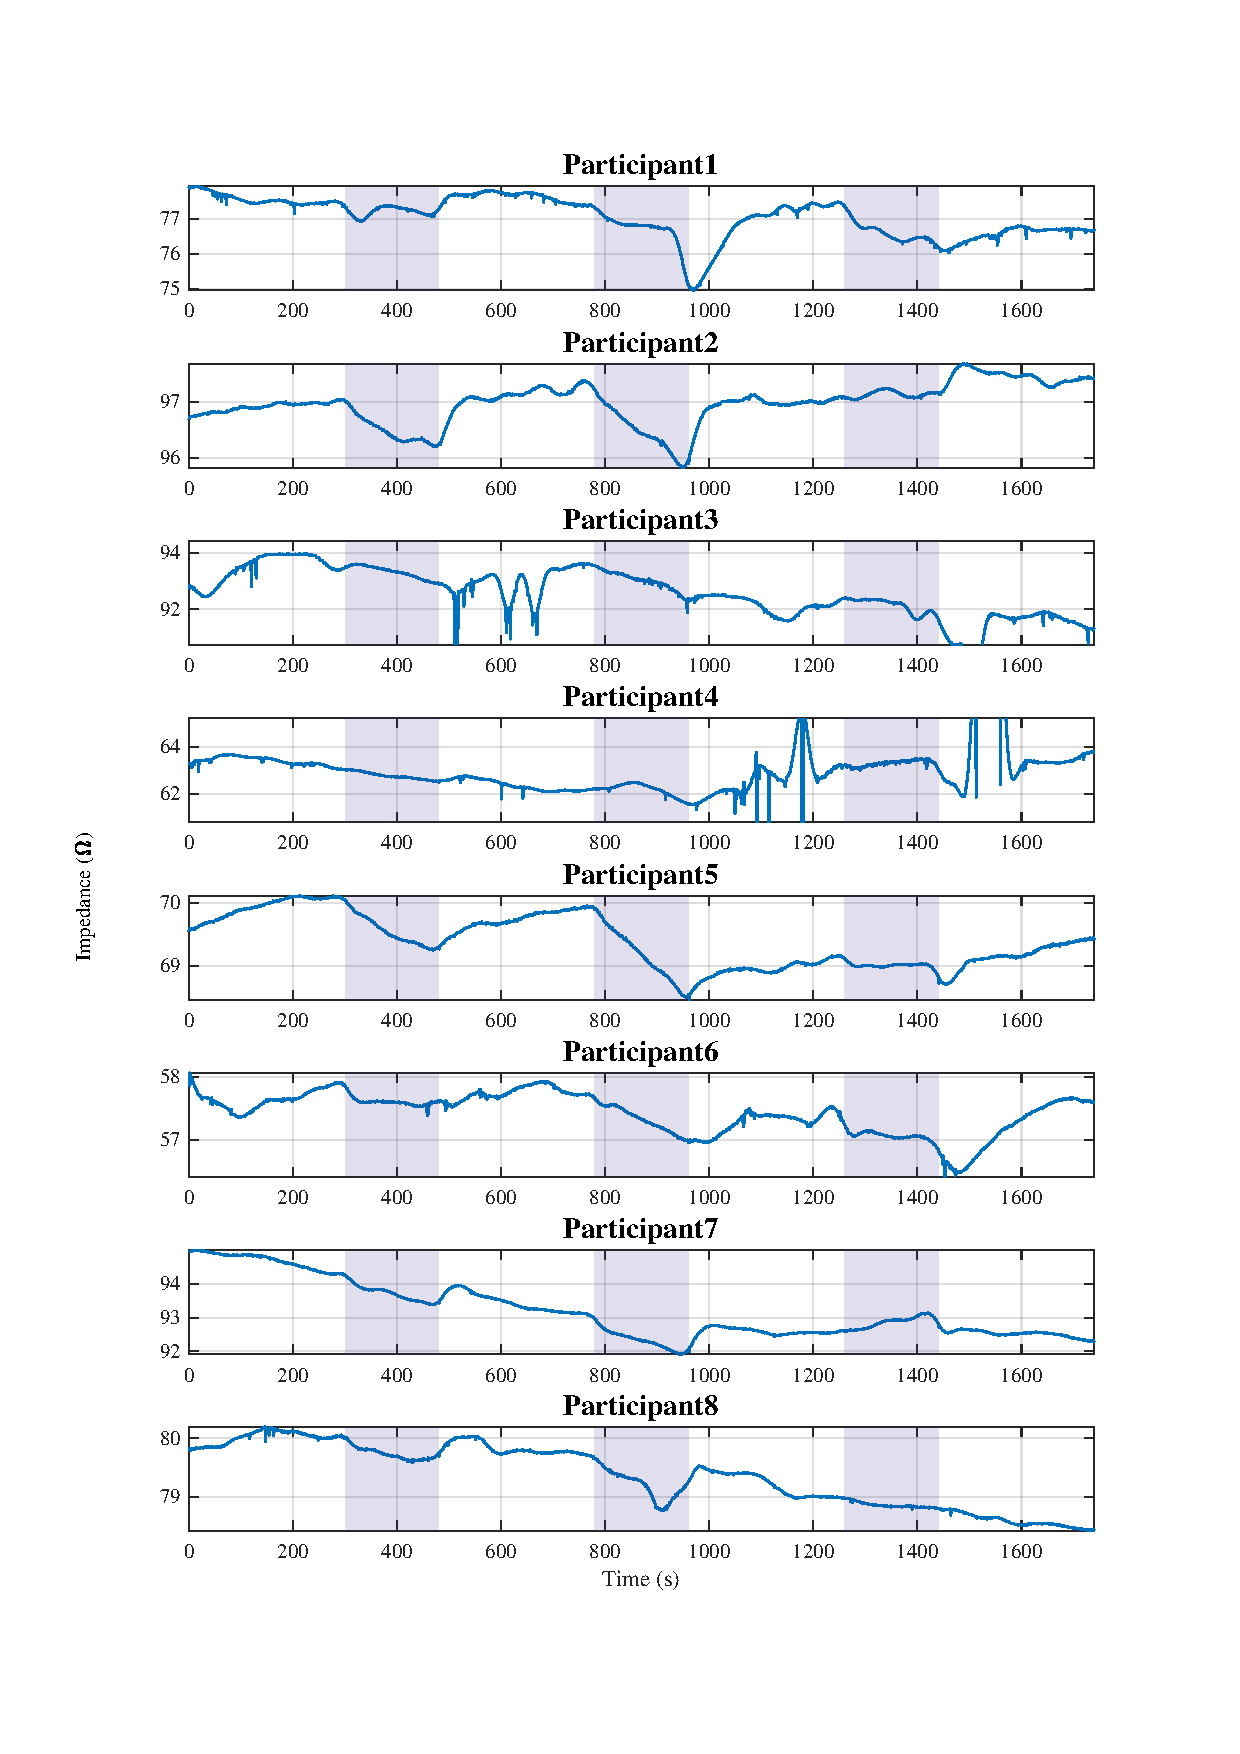
\includegraphics[width=\textwidth,height=\textheight,keepaspectratio]{figure1}    
	\caption{Baseline impedance of all the participants during the study. The shaded areas represent occlusions events.}
	\label{fig:rb:all_participants}
\end{figure}
\todo{This figure is temporary. It needs to be improved by naming axis}


%%********************************** % Section 5.1.1 ******************************************
\subsection{Basal impedance}
\label{section5.1.1}
The iPG device recorded the impedance during the first five minutes of data logging. As described in the previous chapters\todo{Maybe add a reference of the past chapter}, this signal is composed of the base impedance value and the AC waveform signal that is present with it. Moreover, this mean value is known as basal impedance, which it is equivalent to the value $R_B$ described by Nyober's equation \ref{eq:Nyober}. In other words, it is the value of the impedance before the circulation passes through the potential sensors. It is composed basically of the impedance contribution of bone, muscle, fat, skin and residual blood within the vessels. 

The device was able to detect the forearm's segment impedance quite remarkably. The values obtained felt within the resistive value estimated by the literature \todo{Find some papers with results about the impedance of the forearms}. The table \ref{tbl:basal_impedace:region1} describes the basal impedance during the first five minutes of data. 

\begin{table}[b]
	\caption{Basal impedance during the first five minutes of data with statistical values.}
	\label{tbl:basal_impedace:region1}
	
	\centering
	\begin{tabu}{ccccc}
		\hline
		&   \textbf{Mean}   &   \textbf{Variance}   & \textbf{Maximum}  & \textbf{Minimum}  \\ \tabucline[2pt]{-}
		Participant 1 & \SI{77.594}{\ohm} & \SI{\pm0.02752}{\ohm} & \SI{77.374}{\ohm} & \SI{78.038}{\ohm} \\
		Participant 2 & \SI{96.968}{\ohm} & \SI{\pm0.00815}{\ohm} & \SI{96.761}{\ohm} & \SI{97.175}{\ohm} \\
		Participant 3 & \SI{93.537}{\ohm} &  \SI{\pm0.255}{\ohm}  & \SI{92.436}{\ohm} & \SI{94.063}{\ohm} \\
		Participant 4 & \SI{63.437}{\ohm} & \SI{\pm0.03548}{\ohm} & \SI{63.021}{\ohm} & \SI{63.765}{\ohm} \\
		Participant 5 & \SI{69.974}{\ohm} & \SI{\pm0.02730}{\ohm} & \SI{69.562}{\ohm} & \SI{70.198}{\ohm} \\
		Participant 6 & \SI{57.684}{\ohm} & \SI{\pm0.02798}{\ohm} & \SI{57.334}{\ohm} & \SI{58.206}{\ohm} \\
		Participant 7 & \SI{94.719}{\ohm} & \SI{\pm0.05637}{\ohm} & \SI{94.270}{\ohm} & \SI{95.053}{\ohm} \\
		Participant 8 & \SI{80.038}{\ohm} & \SI{\pm0.01250}{\ohm} & \SI{79.824}{\ohm} & \SI{80.303}{\ohm} \\ \hline
	\end{tabu} 
\end{table}    
\todo{This table shows variance which should be better std. Maybe I should run Matlab with datastats command to get a better result. Check paragraph written for clarity that it should be std and not var.}

There are different aspects of the geometry that could affect the impedance reading. There have been several studies where has been demonstrated how the distance between electrodes affects readings\todo{Add reference to studies impedance vs. length}. In the current study showed that impedance was influenced by the forearm's circumference, as well as the distance between the potential electrodes. Figure \ref{fig:C_vs_Z} indicates that there is an inverse relation between circumference and impedance. The smallest the forearm's circumference higher the resistivity. On the other hand, there is a direct relation between the distance between the potential electrodes and the resistivity of the segment as depicted in \ref{fig:l_vs_Z}.

\begin{figure*}[t!]
	\centering
	\begin{subfigure}[t]{0.5\textwidth}
		\centering
		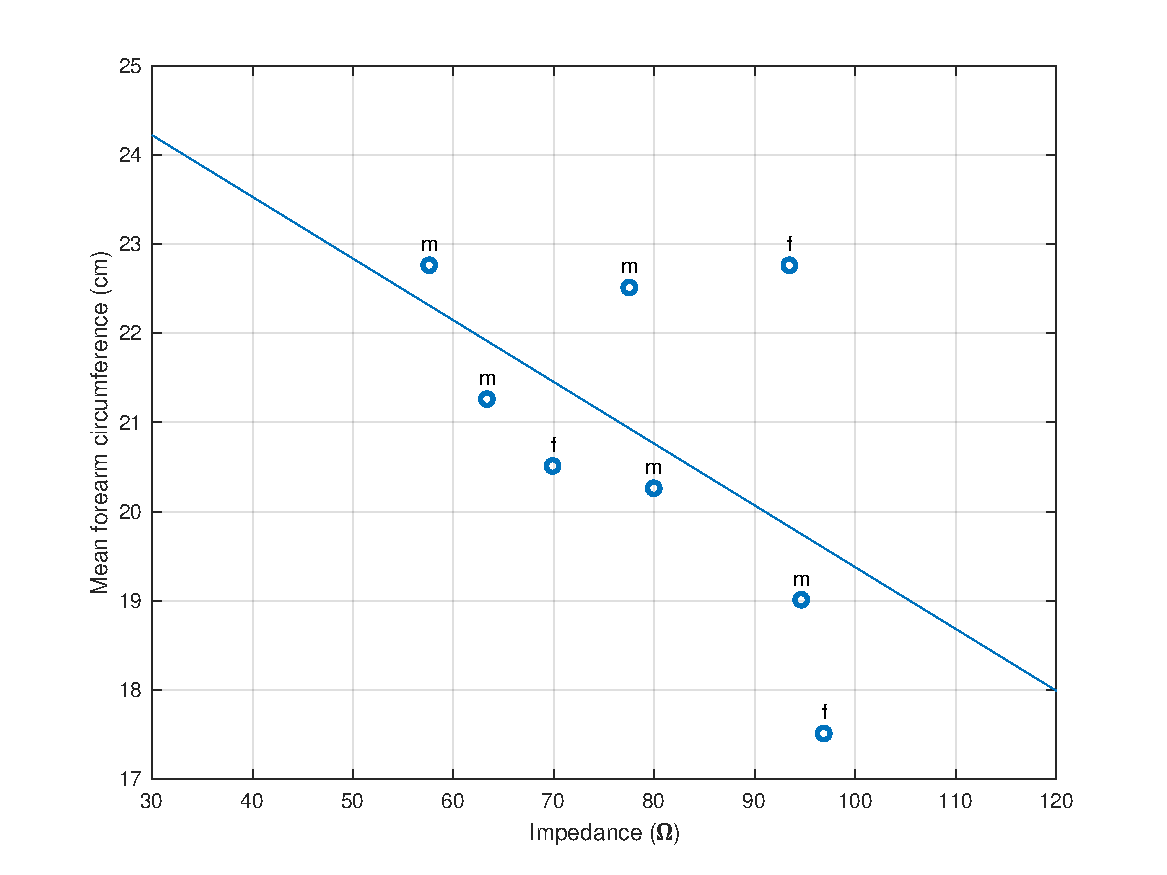
\includegraphics[height=4.5cm]{figure2a}
		\caption{Relation forearm circumference against basal impedance}
		\label{fig:C_vs_Z}
	\end{subfigure}%
	~ 
	\begin{subfigure}[t]{0.5\textwidth}
		\centering
		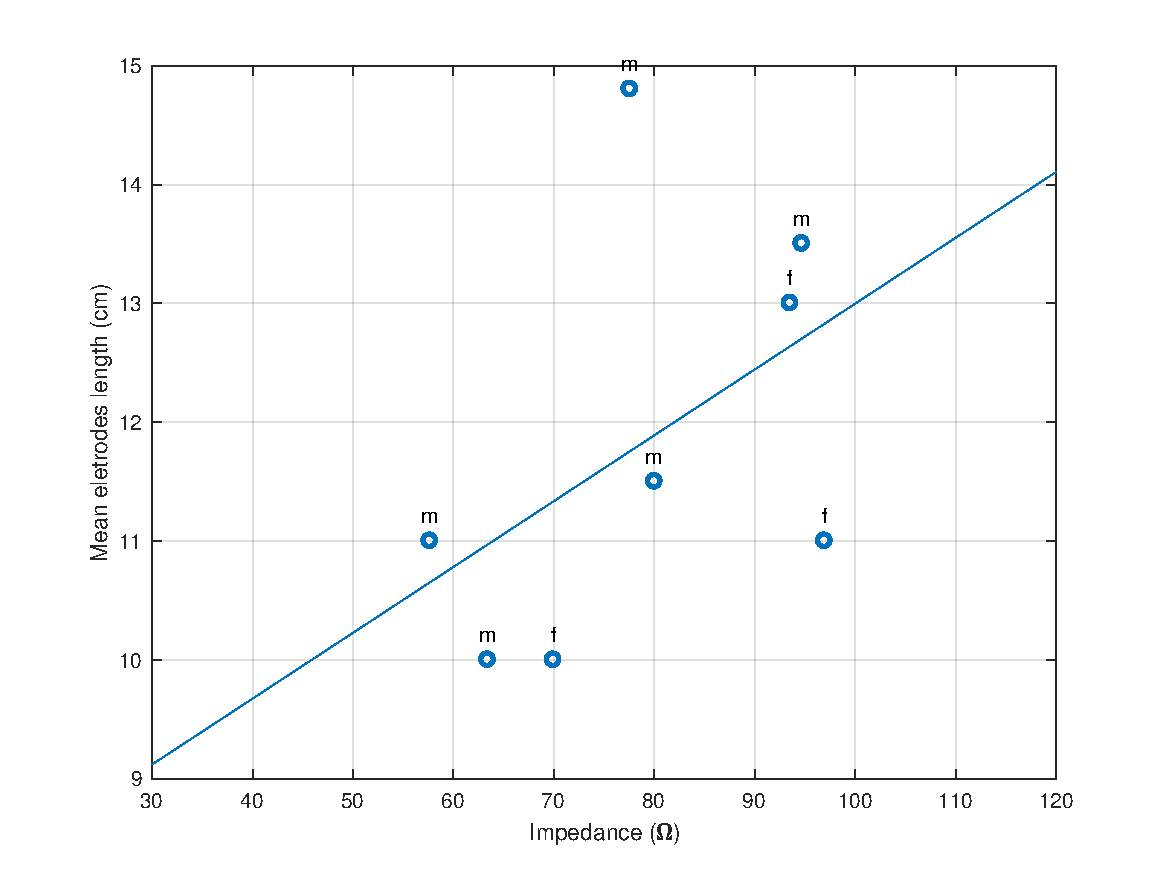
\includegraphics[height=4.5cm]{figure2b}
		\caption{Relation distance sensing electrodes against basal impedance}
		\label{fig:l_vs_Z}
	\end{subfigure}
	\caption{Relation between circumference and length affects basal impedance}
	\label{fig:relation_geometry_vs_impedance}
\end{figure*}


%%********************************** % Section 5.1.2 ******************************************
\subsection{Impedance during venous occlusion}
\label{section5.1.2}
During the following three minutes after the impedance, venous occlusion occurred. As it can be seen in figure \ref{fig:rb:all_participants} all the participants experienced a decrease in basal impedance during this time. Most of the helpers presented a linear impedance decrease trend during the occlusion. However, some of the measurements were clearly affected by motion artefact. Participants one and six are an example of this. 

In participant one, resistance fell off immediately the occlusion occurred. Nevertheless, after a minute the patron moved his arm correcting the trend. Then, impedance continued the trend again. Furthermore,  participant six also showed similar response when the arm moved. 

Figure \ref{fig:normalise:venous_occlusion} describes how the impedance behaved during the occlusion for all participants. The graph has been normalised to compare the resistivity reduction.  A linear regression was performed in the data to demonstrate the ratio of change during the occlusion.  

The table \ref{tbl:venous_occlusion:region2} overviews the results obtained from the linear regression. The value $Z_1$ illustrates the value of the impedance as the blockage started and $Z_{end}$ the resistance value at the end of the test.  $\Delta Z$ (mean $-0.63207 \Omega \pm0.068983\Omega$) is the variation of impedance during the \SI{3}{\minute} that the experiment last.  The slope demonstrates how much resistance is changing during each beat  (mean $-0.0027\Omega\pm3.415e^{-6}\Omega$). 

\begin{figure}
	\centering
	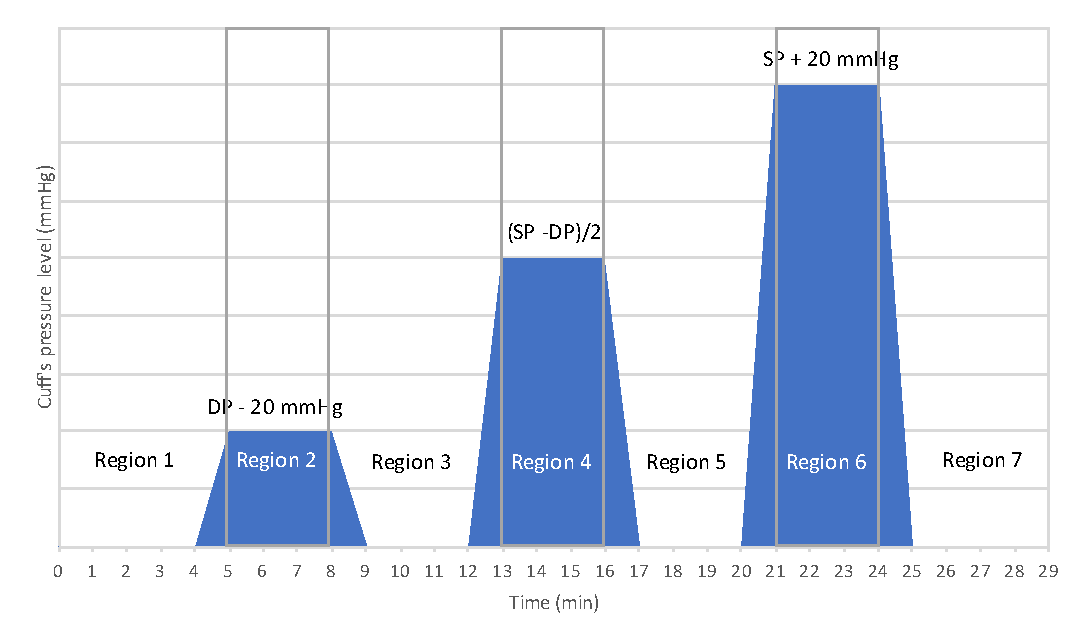
\includegraphics[width=0.9\textwidth,height=0.9\textheight,keepaspectratio]{figure3}    
	\caption{Normalise plot of impedance decrease during venous occlusion.}
	\label{fig:normalise:venous_occlusion}
\end{figure}
\todo{This figure is temporary. It needs to be improved by naming axis}

\begin{table}
	\caption{Basal impedance during the first five minutes of data with statistical values.}
	\label{tbl:venous_occlusion:region2}
	\centering
	\begin{tabu}{lcccccc}
		\hline
		& \textbf{Slope} & \textbf{Intercept} & \textbf{$R^2$} &  \textbf{$Z_1$}   & \textbf{$Z_{end}$} & \textbf{ $\Delta Z$} \\\tabucline[2pt]{-}
		Participant 1 &   0.00056996   & \SI{77.021}{\ohm}  &    0.037341    & \SI{77.491}{\ohm} & \SI{77.184}{\ohm}  & \SI{-0.3077}{\ohm}   \\
		Participant 2 &   -0.0039506   & \SI{98.086}{\ohm}  &    0.86685     & \SI{97.161}{\ohm} & \SI{96.215}{\ohm}  & \SI{-0.9462}{\ohm}   \\
		Participant 3 &   -0.004214    &  \SI{95.01}{\ohm}  &    0.91715     & \SI{93.474}{\ohm} & \SI{92.894}{\ohm}  & \SI{-0.5807}{\ohm}   \\
		Participant 4 &   -0.0029575   & \SI{63.956}{\ohm}  &    0.92013     & \SI{63.218}{\ohm} & \SI{62.609}{\ohm}  & \SI{-0.6091}{\ohm}   \\
		Participant 5 &   -0.0042678   &  \SI{71.26}{\ohm}  &    0.93566     & \SI{70.103}{\ohm} & \SI{69.268}{\ohm}  & \SI{-0.8345}{\ohm}   \\
		Participant 6 &  -0.00084623   & \SI{57.958}{\ohm}  &    0.32203     & \SI{57.979}{\ohm} & \SI{57.575}{\ohm}  & \SI{-0.4045}{\ohm}   \\
		Participant 7 &   -0.004271    & \SI{95.418}{\ohm}  &    0.93423     & \SI{94.325}{\ohm} & \SI{93.341}{\ohm}  & \SI{-0.9849}{\ohm}   \\
		Participant 8 &   -0.0017339   & \SI{80.426}{\ohm}  &    0.75228     & \SI{80.071}{\ohm} & \SI{79.681}{\ohm}  & \SI{-0.3895}{\ohm}   \\ \hline
	\end{tabu} 
\end{table}

From the statistical analysis displayed can be concluded the following. First, as it was explained before, the slopes from participants 1 and 6 were affected by the motion artefact. Nevertheless, these trends seemed corrected after one minute of recordings (\SI{360}{\second}). Their slopes were quite far away from the mean value ($-0.0027089 \Omega$). On the other hand, the rest of the signals showed a similar trend. 


%********************************** % Section 5.2 ******************************************
\section{Blood flow calculation during venous occlusion}
\label{section5.2}
Using the method venous occlusion plethysmography is possible to calculate the blood flow in the forearm segment. As it can be seen from figure \ref{fig:blood_flow:venous_occlusion} the data is not dropping in a completely straight line. As a reminder, the occlusion occurred during \SIrange{300}{480}{\second} which is the time lapse showed. There are impedance variations caused by respiration movement contained within the signals, but also some sections are affected by muscle contraction. If the blood flow was computed using point by point method, there would be some discrepancies when the resistivity is increasing. Thus, this will lead to an incorrect reflection of the blood stream. 

As a result, the method described in section xxx was used to calculate the blood flow between decreasing points only. In short, this algorithm finds the peak and valleys of the signal and then computes the blood flow using equation \ref{eq:QL} between those points found. The figure \ref{fig:blood_flow:venous_occlusion} on the left shows the impedance decrease during the occlusion for all participants. The image on also depicts the points from where the algorithm extracted the reference points for its calculations. In this case, the red triangle pointing downwards is equivalent to the base impedance $R_B$ and the black triangle is the ending point of the calculation point. Then $\Delta R / \Delta t$ can be obtained as the difference between these two points in impedance and time. 
%\todo{Add a section describing how the data was treated.} 

In the same figure but on the right, it can be noticed the result of the blood flow calculated in units of \si{\ml / \min 100 \ml}. The blue dots indicate the instant blood flow at the end value of $\Delta R$. The orange line indicates the mean blood flow during measurements. Again, participants 1 and 6 flow estimation is affected by movement producing a mean value far from the majority of the data points. This is confirmed by examining the results summarised on the table \ref{tbl:blood_flow:region2}. The standard deviation $(\sigma_x)$ is quite far compared to the rest of the participants, as well as the minimum value of the data. Therefore, the results of these two participant clearly cannot be expected being accurate. However, if the data sample was a linear section then the calculated flow will be more in agreement with the expected values. 

From this table can be noticed that the calculated blood flow per \SI{100}{\ml} of tissue for all the participants was in average \SI{-295.42}{\ml / \min 100\ml} $\pm$ \SI{113.6}{\ml/\min 100\ml}. 

\begin{table}[t]
	\caption{Basal impedance during the first five minutes of data with statistical values.}
	\label{tbl:blood_flow:region2}
	\centering
	\begin{tabu}{lcccccc}
		\hline
		& \textbf{Number} & \textbf{Median} & \textbf{Mean} & \textbf{$\sigma_x$} & \textbf{Max} & \textbf{Min} \\\hline
		Participant 1 &       23        &     -489.83     &    -639.54    &       $\pm 569.3$        & -32.627      & -2397        \\
		Participant 2 &       30        &     -153.91     &    -155.28    &       $\pm73.365$        & -31.604      & -338.89      \\
		Participant 3 &       31        &     -324.1      &    -331.17    &       $\pm185.71$        & -5.9507      & -801.2       \\
		Participant 4 &       34        &     -410.72     &    -416.15    &       $\pm261.33$        & -5.6671      & -1081.7      \\
		Participant 5 &       23        &     -204.15     &    -205.86    &       $\pm116.03$        & -20.893      & -584.95      \\
		Participant 6 &       29        &     -325.26     &    -691.89    &       $\pm1209.6$        & -42.098      & -4979.7      \\
		Participant 7 &       25        &     -226.31     &    -241.35    &       $\pm111.71$        & -9.917       & -449.2       \\
		Participant 8 &       42        &     -229.08     &    -270.98    &       $\pm200.47$        & -27.291      & -1038.1      \\\hline
	\end{tabu} 
\end{table}


\begin{figure}
	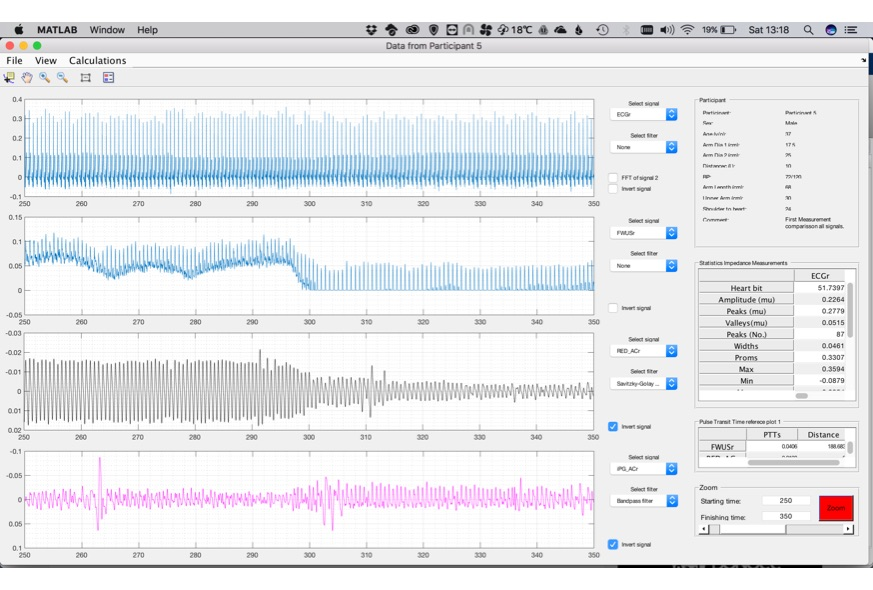
\includegraphics[width=\textwidth,height=\textheight,keepaspectratio,trim={0.5cm 0.5cm 2cm 2cm},clip]{figure4}    
	\caption{Blood flow calculated from venous occlusion plethysmography}
	\label{fig:blood_flow:venous_occlusion}
\end{figure}



%!TEX root = ../thesis.tex
%*******************************************************************************
%*********************************** First Chapter *****************************
%*******************************************************************************

\chapter{Correlations of the impedance plethysmography device}  %Title of the First Chapter
\label{chapter correlations}
\ifpdf
    \graphicspath{{Chapter6/Figs/Raster/}{Chapter6/Figs/PDF/}{Chapter6/Figs/}}
\else
    \graphicspath{{Chapter6/Figs/Vector/}{Chapter6/Figs/}}
\fi

The previous chapter \ref{chapter results} showed the performance of the designed impedance plethysmography device and the data collected in resistivity value and its equivalent in blood flow. It was shown the capability of the instrument on detecting changes during three different kinds of occlusion. Furthermore, it was presented the data collected from the other devices such as Doppler ultrasound, LDF, PPG and ECG. 

In this chapter, the correlation between the different measurements gathered will be analysed. The aim of this correlational investigation is understanding what the contributing factors towards the impedance plethysmography signal are. As it has been explained in previous chapters, the change of the volume in the forearm section let to estimate the blood flow from the segment. However, both arterial and venous blood contributes to the information of blood flow calculated by the iPG device. It is not clear, how much of the blood flow belongs to any of the types of blood. Besides, it was shown that main blood vessels contribute to the measurement of blood flow but microcirculation might also provide additional information under the iPG waveform. 

\mynote{This paragraph is quite an statement. I have to verify if I can really calculate how much is the contribution of the micro circulation and the other types of blood flow.}

%********************************** %First Section  **************************************
\section{Analysis of the the heart beat detection in the frequency domain} %Section - 6.1
\label{section correlation 1} 
The signals obtained from each device all along the experiment are synchronous to the heart beat. This synchronisation reflects that in their dynamic component the systolic peak is also present in the waveform of these instruments.

Nonetheless, some noises impact negatively to the proper detection of the systolic peaks during the study. The algorithm designed can detect the shape of the waveform by finding the foot of the signal and its peaks. Nevertheless, some of the peaks might be missing because of the noise levels.

A Fast Fourier Transform was used to detect the main harmonic of the waveforms in a random window data set. The data selected was between \SIrange{580}{780}{\second} for the AC components only. The algorithm was programmed to detect the frequency peak ($f_p$) from \SIrange{0.85}{1.75}{\hertz}. The FFT was limited to detected frequencies between \SIrange{0}{5}{\hertz} due to the filters applied to the waveforms as explained in section \ref{section procedure 3}.

From Figure \ref{fig:fft signals} can be seen the frequency components from all participants measurements. The ECG plots show the frequency response typical of this kind of signal. Some signals presented a high level of high-frequency components such as the ones seen in participants 1 and 8. The Participant 3 showed a high \SI{2}{\hertz} harmonic peak which power was greater than the first harmonic. This response seems odd but by examining the waveform in detail showed a lower Q wave which might influence the abnormal frequency component presented in the graph.

\begin{figure}[!htpb]
	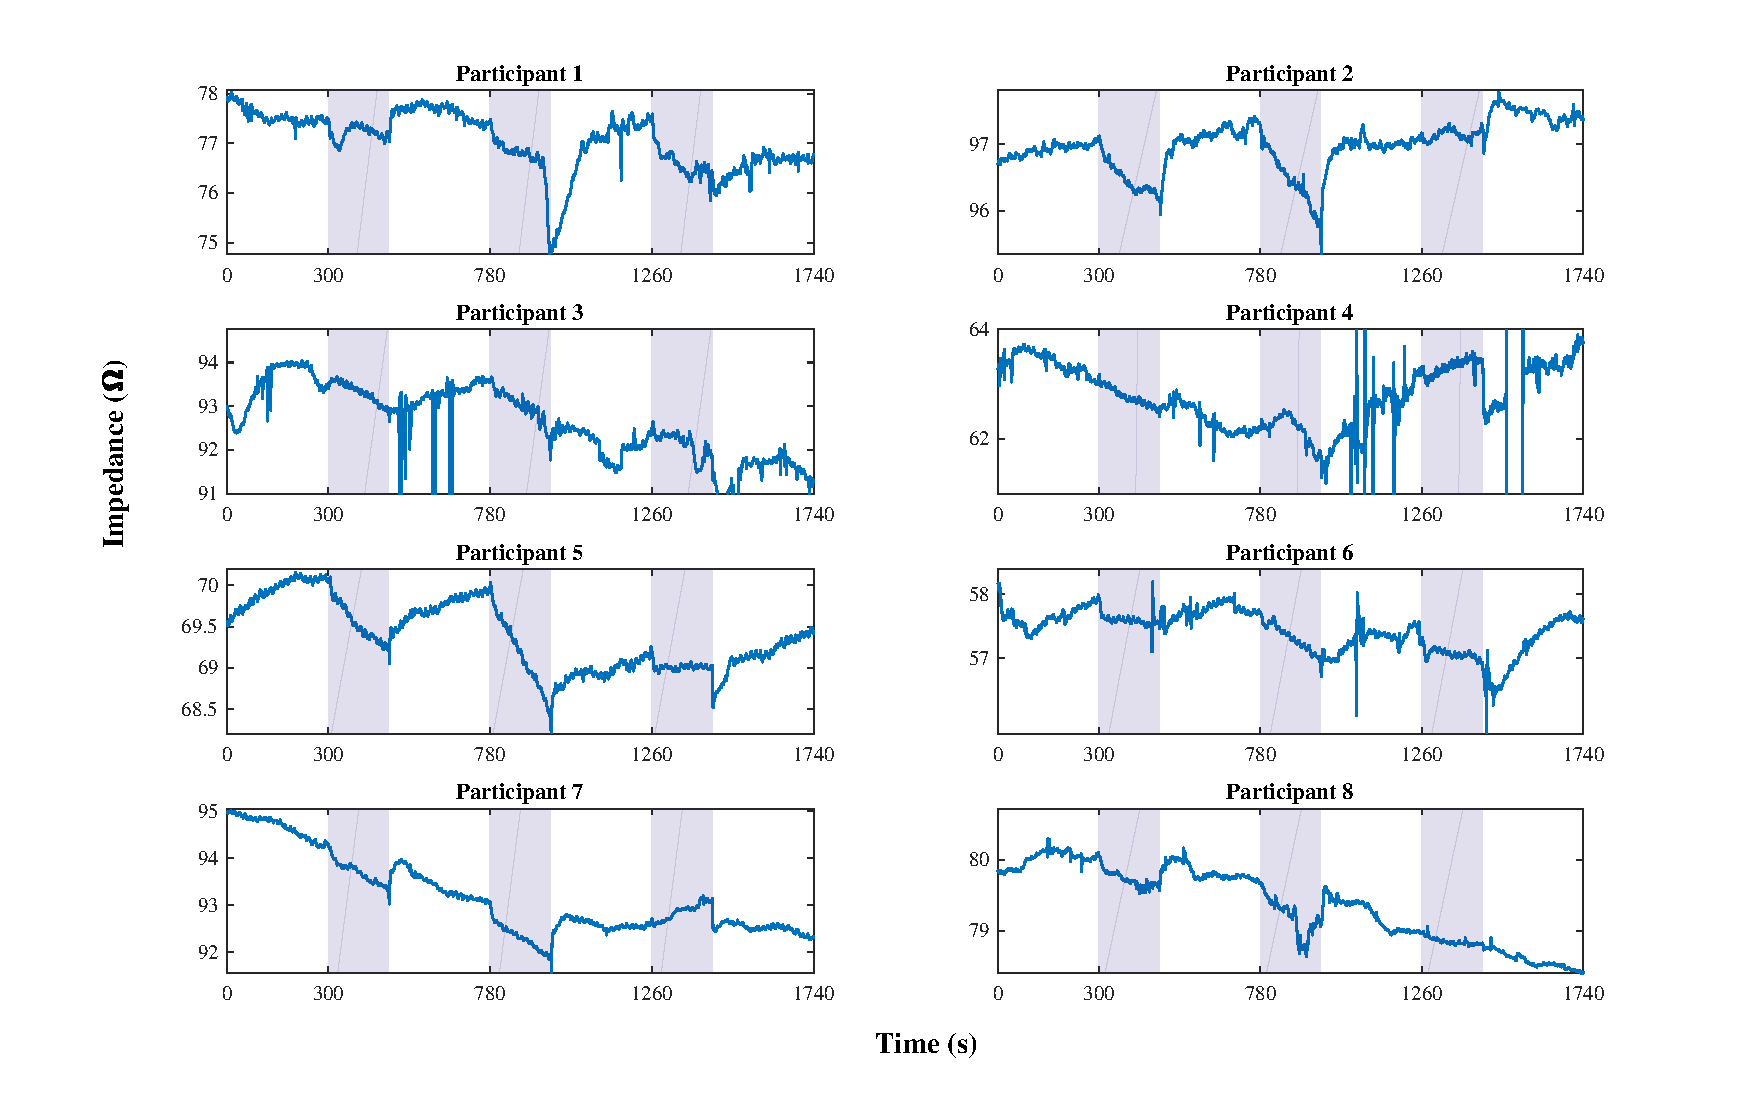
\includegraphics[width=1\textwidth,keepaspectratio,trim={0.75cm 0cm 2cm 2cm},clip]{figure1}    
	\caption[Fequency components of the signals acquired]{Fast Fourier transform for all the measurements in the study. Any DC level was removed previous the FFT. The main harmonic represents the heart frequency. The data range corresponds to the time between \SIrange{580}{780}{\second} for the AC components af the measurements.}
	\label{fig:fft signals}
\end{figure}

The iPG device had a mixed frequency response to detecting the cardiac heartbeat. As it can be seen from the shown plots, some signals show a low-frequency noise which in some cases it is larger than the expected first harmonic. For instance, participants 1, 3 4 and 6 was hard to detect the frequency peak related to the cardiac cycle for this particular data set. However, the rest of the partakers registered a frequency peak at similar heart beat as the ECG. 

PPG frequency components were quite clear in all the participants. Some of them showed high-frequency noise as participant 8. However, in general, this signal shows low signal to noise ration compared to iPG which is understandable as the PPG-AC is significantly larger than the iPG-AC amplitude

Lastly, DU exhibited a clear FFT components in most of the participants. Only Participant 1 demonstrated a high noise component in his measurements but the rest showed a response similar to the ECG. 

Table \ref{tbl:fft} demonstrates how close the cardiac frequency is to each instrument. However, the iPG mean harmonic and frequency distribution from participant 8 illustrates that his data was not clean.


\begin{table}[!htbp]
	\caption[Peak frequency calculated obtained form Fast Fourier Transform]{Cardiac frequency obtained from the Fast Fourier Transform for each of the instruments used during the experiment. This peak corresponds to the one with in the hearth cycle in the study (\SI{0.5}{\hertz} < $f_p$ > \SI{1.5}{\hertz})}
	\label{tbl:fft}
	\centering 
	\begin{tabular}{lccccc}
		\toprule
		& \textbf{ECG}
		& \textbf{iPG}
		& \textbf{PPG}
		& \textbf{LDF}
		& \textbf{DU} \\
		& \textbf{$f_p$ [\si{\hertz}]}		
		& \textbf{$f_p$ [\si{\hertz}]}		
		& \textbf{$f_p$ [\si{\hertz}]}
		& \textbf{$f_p$ [\si{\hertz}]}
		& \textbf{$f_p$ [\si{\hertz}]}\\\midrule
	    Participant 1    &     0.967    &     0.952    &     0.949    &     0.897    &     0.949    \\  
		Participant 2    &     0.964    &     0.964    &     0.989    &     0.964    &     0.964    \\  
		Participant 3    &     1.041    &     0.916    &     1.041    &     1.038    &     1.019    \\  
		Participant 4    &     1.425    &     1.437    &     1.422    &     1.321    &     1.425    \\  
		Participant 5    &     0.940    &     0.940    &     0.937    &     0.940    &     0.940    \\  
		Participant 6    &     1.239    &     1.242    &     1.242    &     1.233    &     1.239    \\  
		Participant 7    &     1.163    &     1.163    &     1.163    &     1.163    &     1.163    \\  
		Participant 8    &     1.346    &     1.401    &     1.337    &     1.367    &     N/A    \\  
 
	\bottomrule
	\end{tabular}
\end{table}


%********************************** %Second Section  *************************************
\section{Correlation between iPG AC waveform and Ultrasound Doppler} %Section - 6.2
\label{section correlation 2} 
The Chapter  \ref{chapter results} showed how the waveforms obtained during the experiment changed in amplitude at each occlusive event. By observing the equation \ref{eq:doppler}  from the Doppler ultrasound section can be derived that the velocity ($v$) is directly proportional to the Doppler frequency ($f_D$). The rest of the terms can be assumed as constant. After that, the same rule obeys when the velocity is converted to blood flow. Equally, the blood flow calculated from the iPG device with equation \ref{eq:bf} is a function of $R_B$ which is a directly proportional to the amplitude of the impedance waveform at the point $R_{M5}$ as shown by equation \ref{eq:RB}. In other words, the magnitude of both measurements changes according to the blood flow.

However, the Doppler ultrasound is only focused on arterial flow over the blood vessel under observation. Instead, iPG sees flow changes of both arterial and venous circulation in the volume segment under test. Both devices measure blood flow but in a different way. The Doppler ultrasound requires precision when placing the head of the instrument on the patient's skin. The best signal is obtained when the device is exactly over the blood vessel. Hence, the clarity of the signal depends on the operator skills to maintain a constant angle and always over the artery. During the experiment, this procedure was replicated using laboratory instruments keeping both angle and skin contact constant. Although, using this set-up does not counter rest the participant's arm movement which causes a misaligning of the sensor. As a result, the amplitude of the ultrasound signal is not as steady as one might expect. 

As it was observed in section \ref{section correlation 1} the AC components of the iPG device is not clean of noise in all the partakers. In fact, participant 2, 5, 6 and 7 showed the best signals to work with. For this reason, the waveforms from these partakers were used when performing the correlation between both instruments. 

Figure \ref{fig:corr FWUS} shows the correlation between both iPG and DU. The data range corresponds to the whole duration of the experiment as includes the changes of blood flow caused by the occlusions. In the plot, the data was discriminated with a different marker point and colour according to every event during the test. As a reminder, odd regions are baselines, and even regions are blockages.  

\begin{figure}[!htpb]
	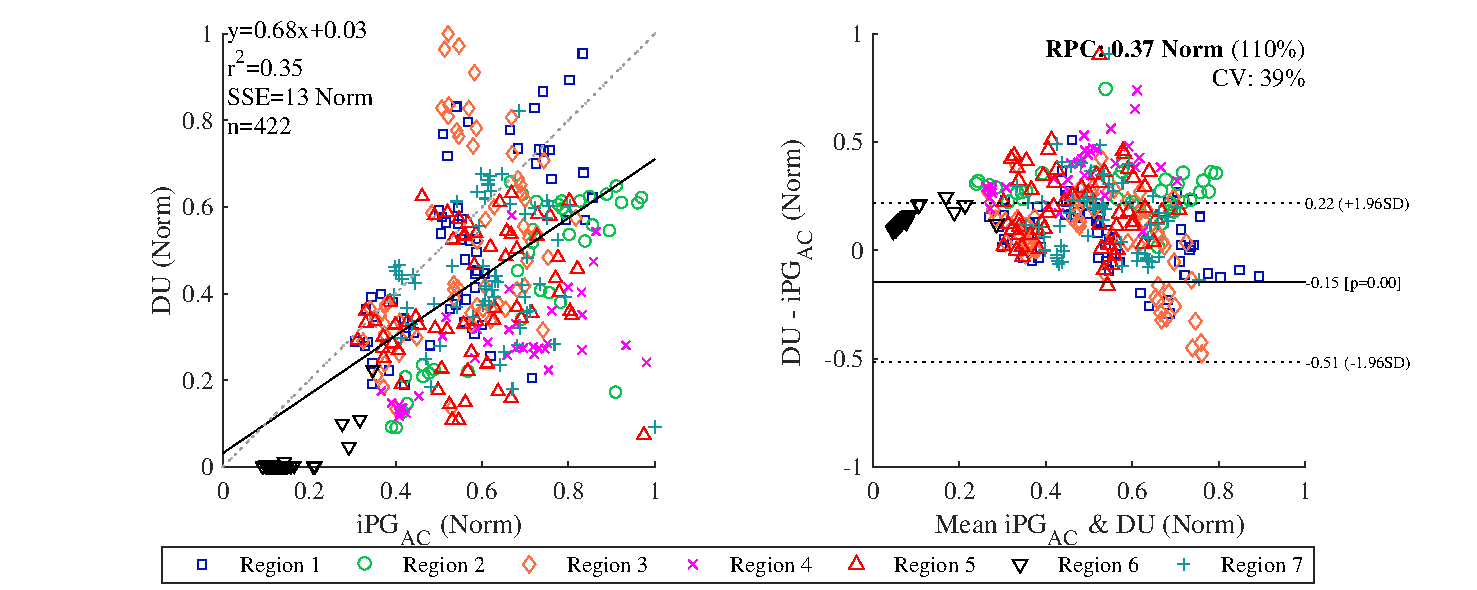
\includegraphics[width=1\textwidth,keepaspectratio]{figure2}    
	\caption[Bland and Altman plot of the relation between Doppler ultrasound and iPG]{Bland and Altman~\cite{bland1986statistical} plot of the relation between Doppler ultrasound and iPG. Data set corresponds to participants 2, 5, 6 and 7.  The data has been normalised comparing the amplitude of both measurements. The different regions has been plotted with various colours and symbols to differentiate every event. The dotted line represents the perfect agreement, the dark line is the linear regression.}
	\label{fig:corr FWUS}
\end{figure}

The data was normalised referenced to the highest peak of the total data set.  Each systolic peak detected from the iPG waveform was used to the find the corresponding Doppler ultrasound systolic peak around the same segment of time. Then the iPG and DU data sets were smoothed by calculating the mean value of every 20 peaks detected in a non-accumulative average.  

The method used to analyse the correlation of both measurements is the method proposed by Bland et al.~\cite{bland1986statistical}. This method allows comparing a traditional technique with a new method. So, it is ideal to compare the measurements between DU and the designed device. This technique is mostly used to compare similar units measurements, for this reason, the data were normalised. Therefore, the comparison will be on the change of magnitude between both modalities.

On the left of the plot can be seen the result of the linear regression between both waveforms. At certain degree the data trend is off the line of equity (dotted line), meaning that there is not a perfect agreement between both methods concerning their amplitudes. In fact, this graph portrays that the linear correlation between both signals with a coefficient correlation  $r^2 = 0.35$ confirming that both signals are related. However, there is not a perfect agreement because of the variability of the reference signal (DU) alongside the y-axes. 

Analysing region by region can be seen how the data points were distributed along the correlation graph. For instance, there seems to be a good distribution of data in both axes in regions 1 and 2. Clearly, both waveforms amplitudes spread quite uniformly. The region 1 appears to be closer to the line of equity than the region 2 when venous occlusion happened. It seems that the magnitude of the DU signal did not change as much as the iPG's ones. Undeniably, the impedance plethysmography device detected changes that the DU could not notice. Which, it is in agreement as the venous occlusion does not alter the arterial flow. 

However, region 3 shows a larger distribution of data points adjacent to y-axes than iPG. Participants movement would have caused this significant variation of the DU amplitude. By reviewing the envelope of the signal on figure \ref{fig:DU_flow} is noticeable that Participant 7 showed the largest waveform amplitudes, this can also be seen in the mean blood flow computed on that same region. In fact, running the data without this participant, the linear regression improves to $r^2 = 0.45$. 

The region 4 displays a similar behaviour as the region 2; there is a good data distribution, but the iPG amplitude changed more than the DU. Nonetheless, there is a greater concentration of data points in the lower region of both axes. This performance would be expected as there is a reduction of arterial blood during this event. The higher data points towards the iPG axes are related to the blood flow rush at the beginning of the occlusion on participant 7, as shown in \ref{fig:blood_flow_plethysmography}.

The region 5 shows a greater distribution of the data adjacent to the iPG axes. On the other hand, there are some data points on the lower part of the DU axes that affect the linear regression in this region. During total occlusion in region 6, there is a better response of the DU device. Here, a significant number of the Doppler's ultrasound data points are set to zero, whereas the data from iPG is mostly distributing among 0 and 0.2. Finally, the Region 7 shows a good distribution adjacent to the line of equity which agrees with some of the other baseline behaviour.

The plot on the right of figure \ref{fig:corr FWUS} shows the precision between the estimated limits of agreement of the whole experiment.  On the y-axes is plotted the mean difference between both measurements and the points of its standard deviation. The differences have normally been distributed in a Gaussian space. Hence \SI{95}{\percent} confidence interval of the difference should lie between  $\pm$1.96SD. This graph shows that there is a high number of points out of $+$1.96SD. However, it can be noticed that values from regions 2 and 4 are outside the agreement region. Confirming, that when an occlusion occurs there is a different response between iPG and DU.


%********************************** % Third Section  *************************************
\section{Correlation between iPG and PPG}  %Section - 6.3 
\label{section correlation 3}
The correlation between iPG and PPG was also investigated looking for amplitude similarities between both signals during the occlusive events. Similarly, the method used in the previous chapter was used to analyse the change of magnitude between both AC waveforms. The two signals represent changes of volume within a part of the body, PPG in the finger and iPG in the forearm. While the PPG reflects blood movement in the blood vessels beneath the skin in a not well-defined volume~\cite{elgendi2012analysis}, iPG provides information about the change of volume by the blood vessels filling up with blood but limited by the sensing electrodes.

However, it must be noted that the PPG method used in this study was very simple compared to more sophisticated methods that might detect changes in venous and arterial flow using other wavelengths, sensor placement or data interpretations. The correlational study of this section looks for understand the changes in amplitude among AC components of both signals. As it was detailed in previous chapters, both signals showed changes in their DC components for the time being occluded. However, the AC part of both signals changed oppositely. While there was a magnitude increment in the iPG waveform all along the occlusions (see \ref{fig:blood_flow_plethysmography}), the PPG waveform showed a decrease in amplitude during these events \ref{fig:RED_PPG}.

As it was shown in figure \ref{fig:blood_flow_plethysmography}) the participant 2 displayed abnormal AC amplitudes in the time of the experiment. Also, as it was detailed in the previous section, participants 2, 5, 6 and 7 showed a better AC response. For this reason, participant's 2 data was not included in the correlation between these two waveforms. The data sets were smoothed by calculating the mean value of every 20 peaks in a non-moving average.

\begin{figure}[!htpb]
	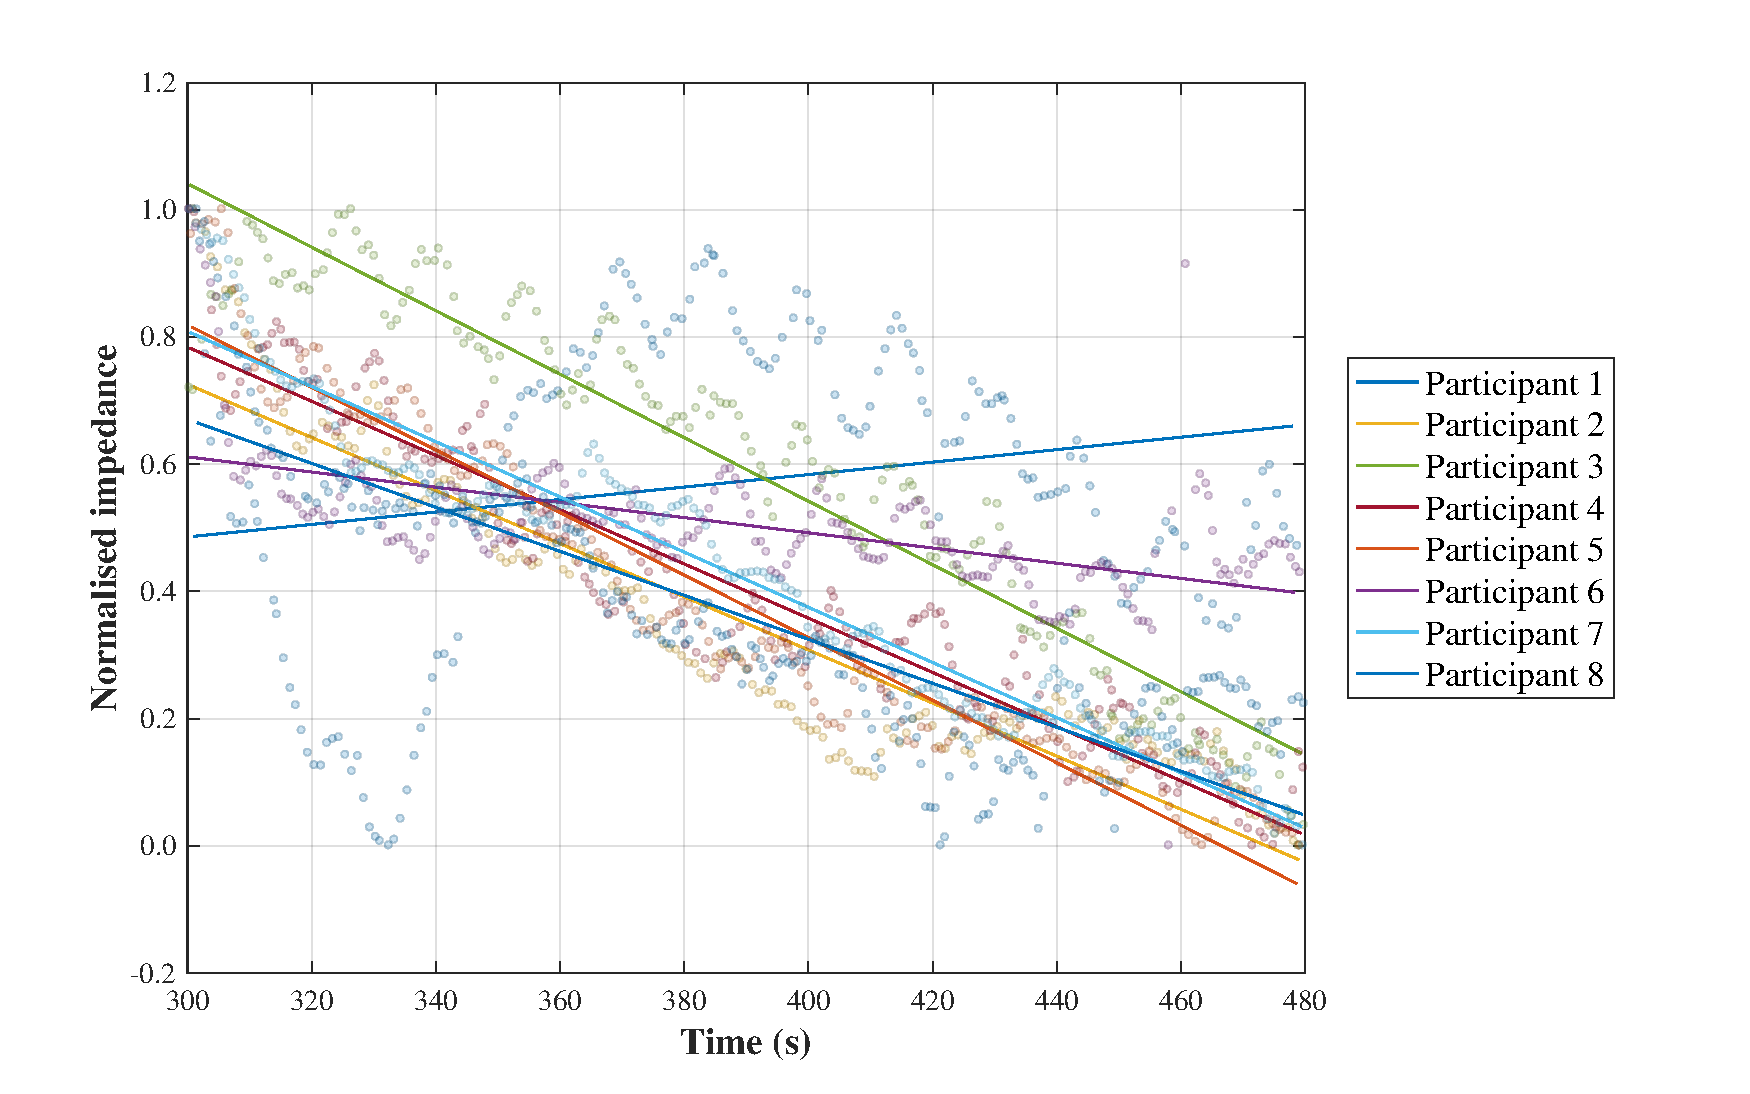
\includegraphics[width=1\textwidth,keepaspectratio]{figure3}    
	\caption[Bland and Altman plot of the relation between PPG and iPG]{Bland and Altman~\cite{bland1986statistical} plot of the relation between PPG and iPG. Data set corresponds to participants 5, 6 and 7. The data has been normalised comparing the amplitude of both measurements. The different regions has been plotted with various colours and symbols to differentiate every event. The dotted line represents the perfect agreement, the dark line is the linear regression.}
	\label{fig:corr RED}
\end{figure}

The Bland et al.~\cite{bland1986statistical} statistical analysis was also implemented in this study. Figure \ref{fig:corr RED} shows the correlation between iPG and PPG magnitudes. From the chart on the left might be seen that there is not a perfect correlation during the whole study, which was expected because the signal's amplitude goes opposite ways all along venous and arterial occlusions. The graph shows a poor linear correlation between both signals with an $r^2 = 0.07$.

Absolutely, most of the baseline data points (regions 1,3,5 and 7) lie closer to the line of equity. In fact, if the venous and arterial occlusive events were removed the correlation between both measurements would improve considerably ($r^2 = 0.40$) . Once more, by analysing the results of this graph is confirmed that the iPG magnitude changed significantly while PPG's amplitude reduced in the course of venous and arterial occlusions. Indeed, it is also verified that the PPG amplitude all along arterial blockage is lower than venous occlusion as portrayed by the data points in the figure. On the other hand, at the time of total occlusion, there was a similar response to both signals, the absence of blood flow translated into small amplitude values. The PPG data points were closer to zero than the iPG magnitudes which were nearer to \num{0.1}.

The BA (Bland and Altman) plot on the left side of figure \ref{fig:corr RED} also illustrates that there was more precision at the time of the baseline readings. Most of the data points are within the \SI{95}{\percent} confidence interval ($\pm $1.96SD), while the measurements during occlusion were mostly outliers.

%********************************** % Third Section  *************************************
\section{Correlation between iPG and LDF}  %Section - 6.4 
\label{section correlation 4}
The signal from the LDF device supplies information about the flow movement of red blood cells in the microvascular network under the skin. However, it is expected a weak correlation between measurements because errors in the data from this instrument have been widely documented especially at low blood flow~\cite{perkash1988difficulties}. Another problem with this technique is that it is not clear if the measurements belong to a venous or arterial flow. 

The position of the LDF sensor head helps to understand the blood flow under microvascular bed under the forearm. As described in section\ref{section procedure 1.1}, the sensor was placed on the forearm midpoint between the iPG's sensing electrodes. 

The signal from the LDF device is similar to a plethysmography wave which is formed by an AC component on a DC signal. For the correlation analysis of this study, the DC component of the signal had to be removed, leaving only the comparison between of normalised AC magnitudes of the LDF and iPG signals. Likewise, as in the previous analysis, the data was smoothed by taking the average value of 20 data points. In the end, the data depicted belongs to participants 2,5,6 and 7.

Figure \ref{fig:corr LDF} shows the linear regression and  BA analysis between both signals. As it might be appreciated, the data points show a poor correlation among both signals ($r^2 = 0.08$). Most of the data points are far from the line of equity and mostly spread across the plot's x-axis. The data points from the LDF signal are not well scattered around the figure. This imbalance can be noticed mostly in the region 7.  An explanation of this effect is that the LDF's peak extension is affected by the hyperaemic effect after the total occlusion has been released, as shown in figure \ref{fig:LDF_flow}. Nonetheless, if this data were removed from the plot still would be a weak agreement between both signals ($r^2 = 0.08$).

From the BA chart on the right side of the figure, it can be noted that there is poor accuracy when comparing the amplitude of both measurements. Therefore, it can be concluded that it is not possible to establish any relation within the magnitude waveform of these two instruments.

\begin{figure}[!htpb]
	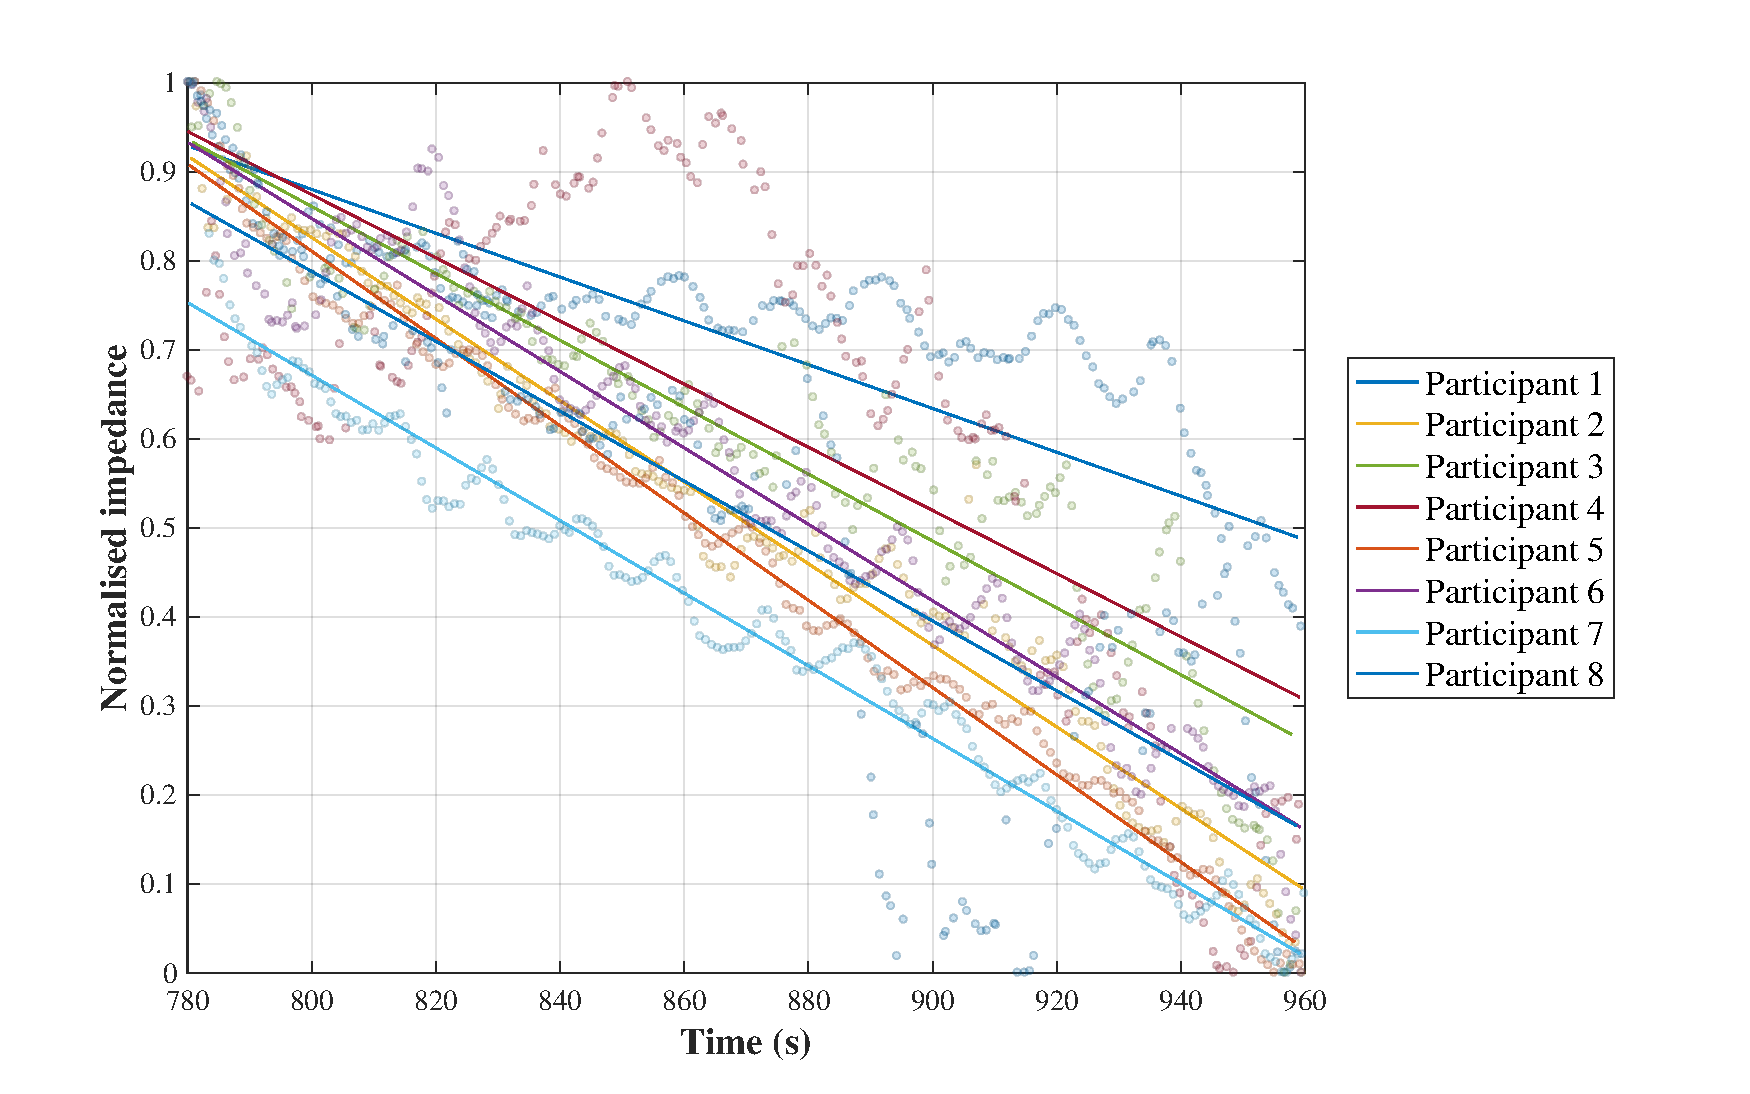
\includegraphics[width=1\textwidth,keepaspectratio]{figure4}    
	\caption[Bland and Altman plot of the relation between LDF and iPG]{Bland and Altman~\cite{bland1986statistical} plot of the relation between LDF and iPG. Data set corresponds to participants 2, 5, 6 and 7. The data has been normalised comparing the amplitude of both measurements. The different regions has been plotted with various colours and symbols to differentiate every event. The dotted line represents the perfect agreement, the dark line is the linear regression.}
	\label{fig:corr LDF}
\end{figure}

%********************************** %Nomenclature found  *************************************
\nomenclature[z-ecg]{FFT}{Fast Fourier Transform}
\nomenclature[z-baa]{BA}{Bland and Altman}
%%!TEX root = ../thesis.tex
%*******************************************************************************
%*********************************** Seventh Chapter *****************************
%*******************************************************************************

\chapter{Research of the change of baseline impedance during proximal occlusion of the limb}  %Title of the First Chapter
\label{chapter occlusion}

\ifpdf
\graphicspath{{Chapter7/Figs/Raster/}{Chapter7/Figs/PDF/}{Chapter7/Figs/}}
\else
\graphicspath{{Chapter7/Figs/Vector/}{Chapter7/Figs/}}
\fi


%!TEX root = ../thesis.tex
%*******************************************************************************
%*********************************** Sixth Chapter *****************************
%*******************************************************************************

\chapter{Research of the shape changes of the arterial pulses during proximal occlusions}  %Title of the First Chapter
\label{chapter apa}

\ifpdf
\graphicspath{{Chapter8/Figs/Raster/}{Chapter8/Figs/PDF/}{Chapter8/Figs/}}
\else
\graphicspath{{Chapter8/Figs/Vector/}{Chapter8/Figs/}}
\fi

The arterial pulses amplitude (APA) are the dynamic component of the impedance plethysmography signal. It lies within the basal impedance which represents about \SI{0.1}{\percent} of the total waveform \cite{anderson1984impedance}. Acquiring these signals can be quite challenging as noise levels could be higher than the actual signal making tough to isolate this waveform. However, obtaining this data provides valuable information about haemodynamics per heartbeat. It has been demonstrated that the shape of the waveform is an indicator of haemodynamic problems in the peripheral circulation. In this chapter, the analysis of the signals aims to differentiate morphological changes between baseline signals and the ones during venous, partial arterial and total occlusion.

As it has been described in the previous chapter, there is a shift in the impedance's baseline during each occlusion. However, it is desirable to study the effect that the different kind occlusions of the upper arm produce in the plethysmography waveforms.  This information may provide clues whether an occlusion may be occurring in either the venous or arterial circulation.  The designed iPG device supplies an output port denominated $Z_{AC}$ \mynote{To double check if this is the correct port name from the initial description} which provides a high-resolution view of the arterial pulses waveform.  In fact, as shown in the design section \ref{section design 1.5}, the signal was filtered and amplified nearly 2500 times to achieve this level of detail. Hence, the waveform obtained provides more in-depth detail and also improves the noise rejection of the signal.

The device produced an excellent result regarding filtering and isolation of the APA waveform. However, undoubtedly some of the noise was also amplified by the hardware. Therefore, further post-processing was required to clean up the plethysmography signal completely. Tighter filters (see table \ref{table:filters}) were applied to remove high and low frequency components. Also, the lower envelope component was also removed and levelled to zero. 

The APA waveform produced by the device is inverted as represented by various other plethysmography method such as photoplethysmography. During the systolic cycle, the blood vessels expand allowing more blood volume. Hence, the impedance drops proportionally to the amount of blood because the forearm's segment is more electrically conductive. On the other hand, during the diastolic cycle, blood vessels empty causing a reduction the quantity of blood contained in the segment. As a result, the impedance increases. 

The analysis of the plethysmographic wave was performed by averaging the waveforms detected using specialized algorithms able to identify an APA signal. The following section discusses the change of wave shape from a non-occlusion state to an occluded one. At the end of the section, the results of all participants are summarised \mynote{I could add a description of how the signal looks. For instance by adding 10 or 20 beats to show how the device worked.}

%%********************************** % Section 8.1 ******************************************
\section{Dataset for the arterial amplitude analysis}
\label{section apa 1}
The isolated APA waveforms reproduce the change of volume per heart beat within the sensing electrodes of the iPG device placed in the forearm. The filling of the vessels with blood produces small changes in resistivity that vary with the circulatory cycle (see section \ref{section impedance 9.1}), describing different peaks during a heart cycle. 

\begin{figure}[!htpb]
	\centering
	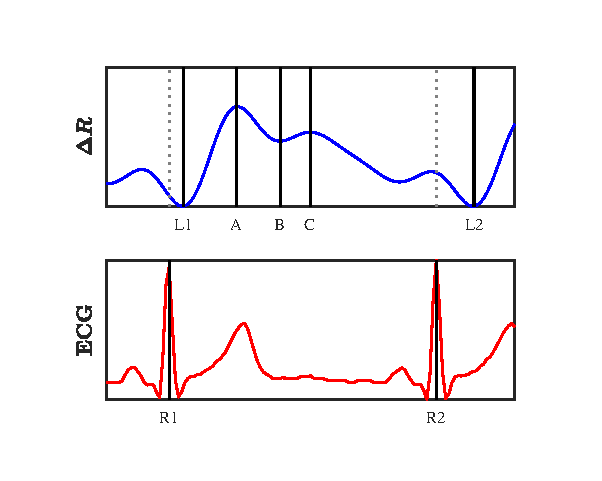
\includegraphics[width=10cm,keepaspectratio]{figure_apa_1}    
	\caption[Marker ppoints in an iPG waveform]{Peaks and valleys of an iPG waveform ($\Delta R$) compared to ECG waveform.}
	\label{fig:markers iPG}
\end{figure}

Commonly, an APA wave consists of several identifiable peaks and valleys. Figure \ref{fig:markers iPG} shows a typical impedance plethysmography pulse synchronous with a heartbeat along with a limb. The table \ref{tbl:APA markers} summarises the noticeable markers of the pulse waveforms when compared with an ECG.

\begin{table}[!htpb]
	\caption{Markers on the APA waveform}
	\label{tbl:APA markers}
	\centering
	\begin{tabular}{c p{10cm}}
		\textbf{Marker} & \textbf{Description} \\
		\toprule 
		R1 & Peak of the ECG QRS complex before an APA pulse. \\ 
		L1 & Start of the systolic upslope of the APA signal. Point where  rapid change of impedance occurs. \\ 
		A & Systolic point. Maximum peak of the APA signal.  \\ 
		B & Dicrotic notch on the APA wave. \\ 
		C & Maximum pulse after the dicrotic notch, named diastolic pulse  \\ 
		R2 & Peak of the ECG QRS complex after the APA pulse.  \\ 
		L2 & Starting point of the next APA wave. \\ 
		\bottomrule
	\end{tabular}
\end{table} 

An APA wave has to be identified as a valid one to be included in the computational analysis. Therefore, the programmed algorithm starts through the identification of the beginning and the end of a pulse by locating the upslope point $L1$ and $L2$ in the waveform. Once this spot has been identified, the systolic peak $A$ can be placed. Follow, the point $B$ is expected to be a valley with an amplitude below the previous peak. Then, the algorithm looks the following change of slope which is the diastolic peak $C$. In case that any of these conditions were not met, then the algorithm searches the APA wave from the next lower data point, looking for a matching wave pattern again. If a pattern is found ($L1 > A < B > slope change (C) > L2$), then this is count as a fixed wave. If there not match the pulse is marked as missing. Also, to minimise waves with abnormal amplitudes caused by noise, the algorithm calculates the mean peak at $A$ of the last 20 valid APA waves. If the value is greater than \SI{25}{\percent} ($A > A*1.25$) then the wave is discarded.  

The table \ref{tbl:detect APA} compiles the amount of APA waves recognised by the algorithm. The column \textit{detected waves} describes the pulses that comply with the profile of an iPG plethysmography wave. The third column shows the pulses that did not match the expected guide; then the algorithm tried to fix them by identifying the pattern in the next slope. As a result, the fixed column shows the total of pulse identified and the last column the ones discarded.

In general, the quality of the APA pulses validated by the iPG device and verified by the algorithm were in average \SI{57.86(1637)}{\percent}. Participants 3, 4 and 8 displayed the highest number of pulses with errors (above \SI{50}{\percent}). However, by performing the fixing method the amount valid peaks improved to a total of \SI{84.94(764)}{\percent}.

\begin{table}[!htbp]
	\caption{Change of amplitude of the waveform at peak A during the transition from baseline to venous occlusion.}
	\label{tbl:detect APA}
	\centering\small
	\begin{tabular}{lrrr>{\columncolor[gray]{0.8}}l>{\columncolor[gray]{0.9}}l}
		\toprule
		& \multicolumn{1}{c}{\textbf{Total}}
		& \multicolumn{1}{c}{\textbf{Detected}} & \multicolumn{1}{c}{\textbf{Waves}}& \multicolumn{1}{c}{\textbf{Fixed}} & \multicolumn{1}{c}{\textbf{Discarded}} \\
		& \multicolumn{1}{c}{\textbf{valleys}} & \multicolumn{1}{c}{\textbf{waves}} & \multicolumn{1}{c}{\textbf{with errors}}& \multicolumn{1}{c}{\textbf{waves}} & \multicolumn{1}{c}{\textbf{waves}} \\
		\midrule
		Participant 1	&1604	& 840 (\SI{52.37}{\percent})	&764 (\SI{47.63}{\percent})	&491 (\SI{30.61}{\percent})	&273 (\SI{17.02}{\percent})\\
		Participant 2	&1689	&1159 (\SI{68.62}{\percent})	&530 (\SI{31.38}{\percent})	&409 (\SI{24.22}{\percent})	&121 ( \SI{7.16}{\percent})\\
		Participant 3	&1651	& 699 (\SI{42.34}{\percent})	&952 (\SI{57.66}{\percent})	&695 (\SI{42.10}{\percent})	&257 (\SI{15.57}{\percent})\\
		Participant 4	&1625	& 645 (\SI{39.69}{\percent})	&980 (\SI{60.31}{\percent})	&562 (\SI{34.58}{\percent})	&418 (\SI{25.72}{\percent})\\
		Participant 5	&1664	&1199 (\SI{72.06}{\percent})	&465 (\SI{27.94}{\percent})	&345 (\SI{20.73}{\percent})	&120 ( \SI{7.21}{\percent})\\
		Participant 6	&1745	& 936 (\SI{53.64}{\percent})	&809 (\SI{46.36}{\percent})	&471 (\SI{26.99}{\percent})	&338 (\SI{19.37}{\percent})\\
		Participant 7	&1907	&1654 (\SI{86.73}{\percent})	&253 (\SI{13.27}{\percent})	&146 ( \SI{7.66}{\percent})	&107 ( \SI{5.61}{\percent})\\
		Participant 8	&1651	& 784 (\SI{47.49}{\percent})	&867 (\SI{52.51}{\percent})	&491 (\SI{29.74}{\percent})	&376 (\SI{22.77}{\percent})\\
		\bottomrule
	\end{tabular}
\end{table}

From these data, the changes during each occlusion among the points $A$, $B$ and $C$  were examined. The following analysis centres in the changes of impedance amplitude all along the different regions of the experiment, and the change of area of the waveform before and after the dicrotic notch point ($B$).

%%********************************** % Section 8.2 ******************************************
\section{Plethysmography waveform change during venous occlusion plethysmography}
\label{section apa 2}
The analysis performed in this section corresponds to the APA waveforms captured during baseline in region 1 (\SIrange{0}{300}{\second}), venous occlusion (\SIrange{300}{480}{\second}) and return to control signal (\SIrange{480}{780}{\second}).  The previous section described the method how the valid pulses were collected. Consequently, all the valid pulses were grouped and aligned per region calculating the average waveform. 

Figure \ref{fig:iPG_venous_baseline} shows an impedance plethysmography waveform calculated from one of the participants during baseline and venous occlusion, with indicators of their amplitudes at the different points of interest. Some of the markers show the calculation of the distance between systolic peak (Point A) to dicrotic notch (Point B) and diastolic peak (Point C), as well as, the amplitude for each of these markers. The distance between (A $\rightarrow$ B) and (A $\rightarrow$ C) was later transposed into the occlusion wave to identify their values during the VOP test.

Clearly,  from a qualitative point of view, one can notice that there is a difference in the morphology of the waveform during the occlusion.  Indeed, figure \ref{fig:iPG_change_points_venous} shows the change of the amplitude at these points for every participant and the return to baseline after the cuff pressure was released. A complete analysis of the change at each point is detailed as follows.

%This method allows multifigures being aligned using subcaptionbox
\begin{figure*}
	\centering
	\null\hfill%
	\subcaptionbox{Average APA waveform for baseline region 1 (\SIrange{0}{300}{\second})\label{fig:iPG_venous_baseline}}
	[0.48\textwidth]{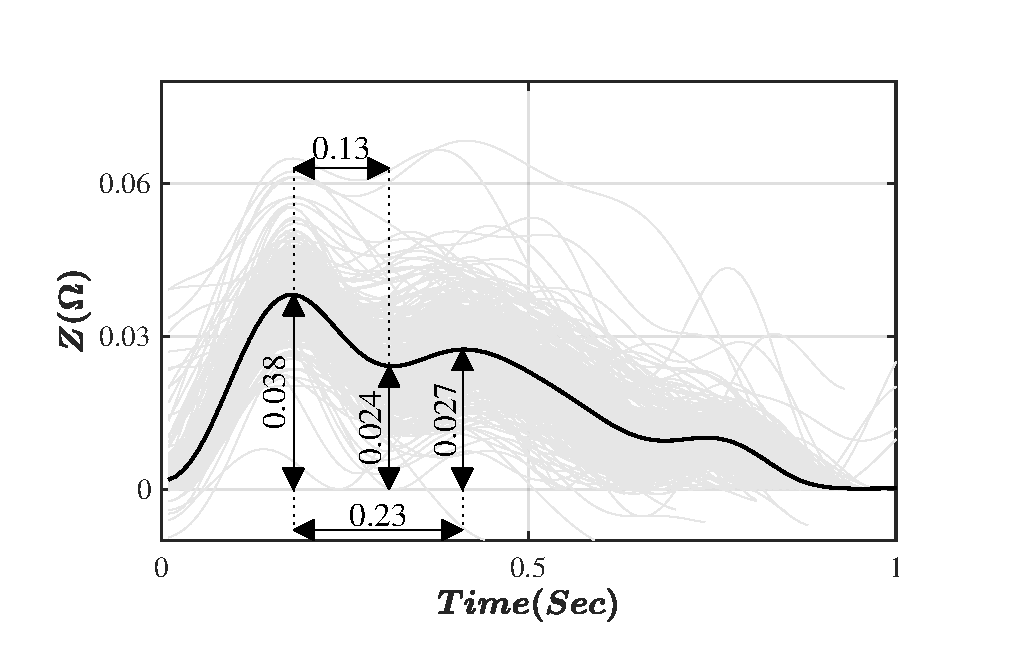
\includegraphics[width=0.48\textwidth, trim={0.5cm 0cm 1.5cm 0 cm}, clip]{figure_apa_2a}}%
	\hfill%
	\subcaptionbox{Average APA waveform during venous occlusion region 2 (\SIrange{300}{480}{\second})\label{fig:iPG_venous_occlusion}}
	[0.48\textwidth]{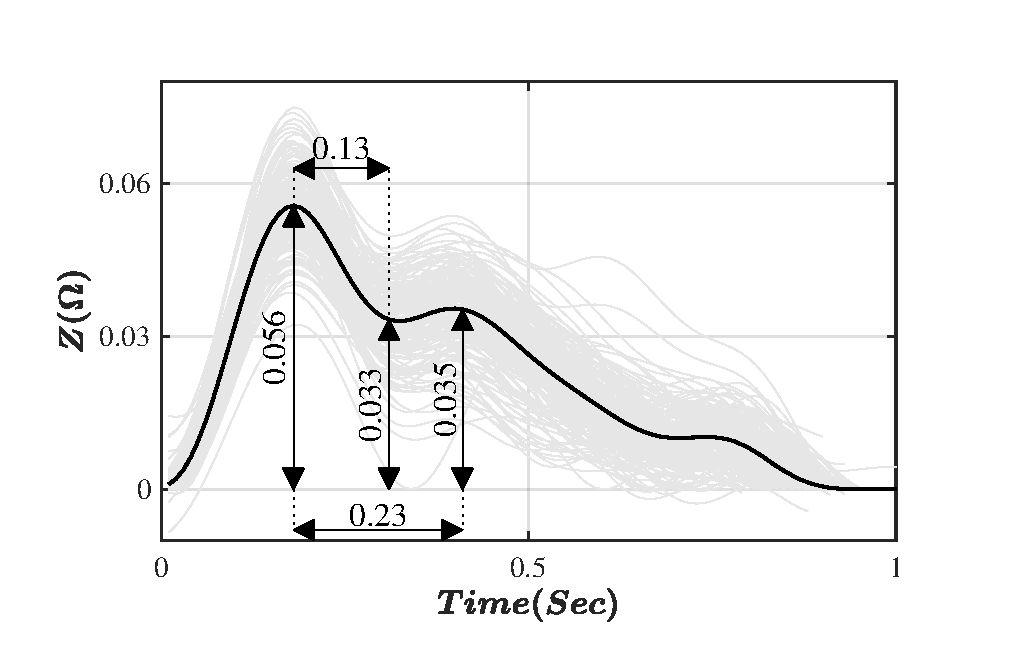
\includegraphics[width=0.48\textwidth, trim={0.5cm 0cm 1.5cm 0 cm}, clip]{figure_apa_2b}}%
	\hfill\null%
	\caption{Plethysmography waveform of the participant seven between baseline and venous occlusion}
	\label{fig:iPG_venous}

	\vspace{1cm}

	\null\hfill%		
	\subcaptionbox{Change of amplitude of the waveform at point A.\label{fig:change A venous}}
	[0.48\textwidth]{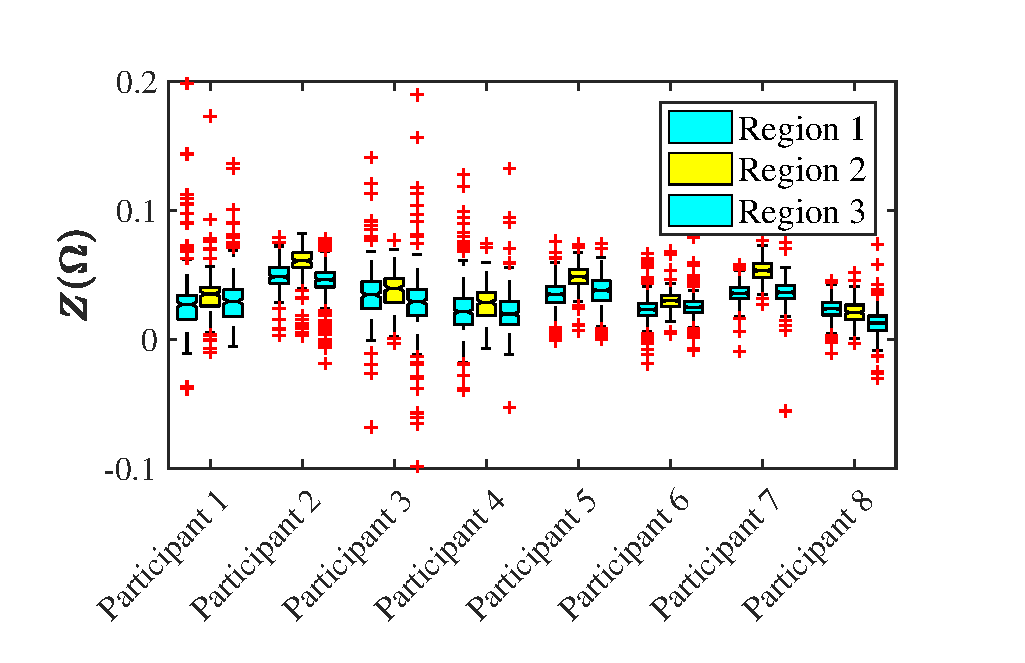
\includegraphics[width=0.48\textwidth, trim={0.5cm 0cm 1.5cm 0 cm}, clip]{figure_apa_3a}}%
	\hfill%
	\subcaptionbox{Change of amplitude of the waveform at point B.\label{fig:change B venous}}
	[0.48\textwidth]{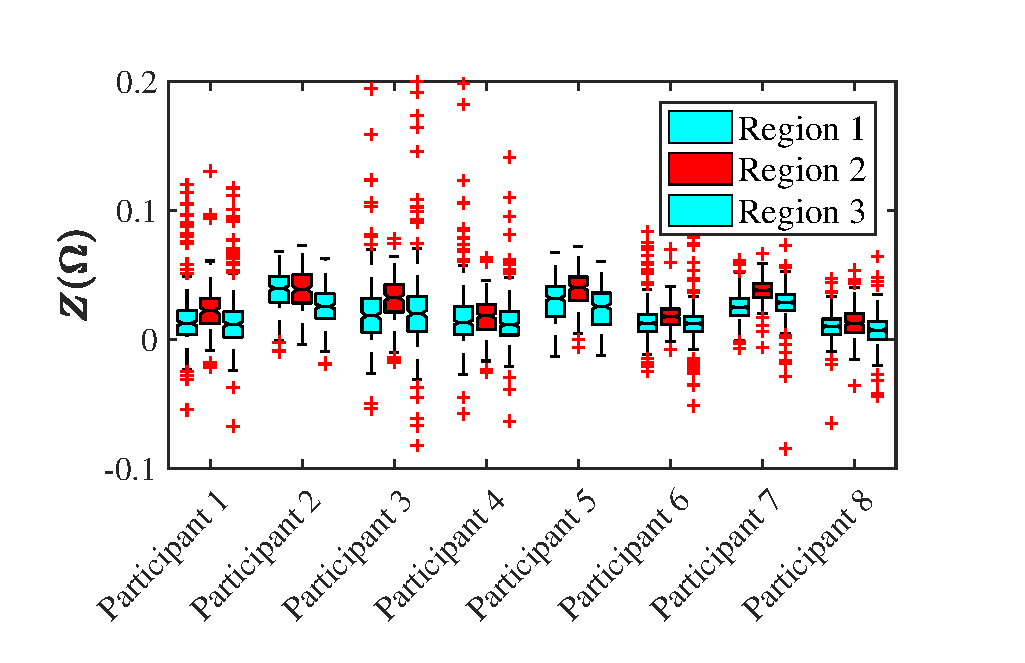
\includegraphics[width=0.48\textwidth, trim={0.5cm 0cm 1.5cm 0 cm}, clip]{figure_apa_3b}}%
	\hfill%
	\subcaptionbox{Change of amplitude of the waveform at point C.\label{fig:change C venous}}
	[0.48\textwidth]{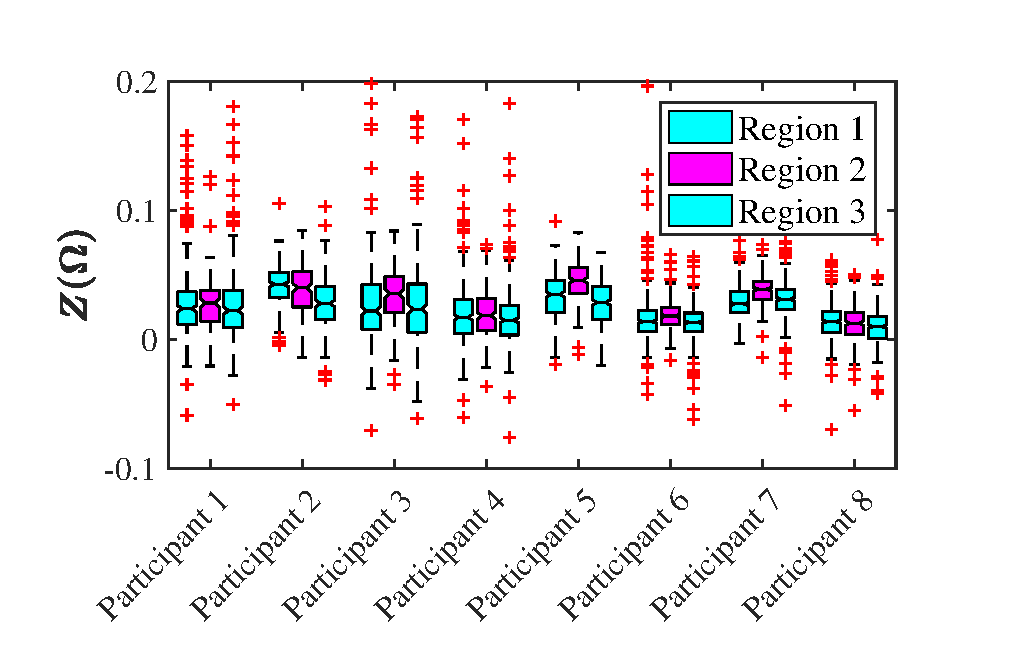
\includegraphics[width=0.48\textwidth, trim={0.5cm 0cm 1.5cm 0 cm}, clip]{figure_apa_3c}}%
	\null%
	\caption{Changes of the impedance peak values during baseline, venous occlusion and return to baseline for points A,B and C.}
	\label{fig:iPG change points venous}
\end{figure*}



\subsubsection{Changes in systolic peak (Point A)}
\label{section apa 2.1}
Figure \ref{fig:change A venous} shows the statistical variation of the systolic peak magnitude (point A) during the three conditions of the test baseline-occlusion-baseline. After inflating the cuff below the diastolic pressure, most of the APA signals displayed an increase of the impedance magnitude of this peak. Indeed, as detailed in table \ref{tbl:change A venous}, \SI{87}{\percent} of the participants showed an increment in electrical resistance during venous occlusion of about \SI{31.80}{\percent}, only participant 8 was an exception where his/her impedance decreased in \SI{-12.01}{\percent}. Then, when the cuff's pressure was released, all the participants showed a decline of the peak value with an average of \SI{-32.21}{\percent}, returning to similar baseline values before the venous occlusion. 

\begin{table}[!htbp]
	\caption[Change of amplitude of the waveform at peak A during the transition baseline-venous occlusion-baseline.]{Change of amplitude of the waveform at peak A during the transition from baseline (region 1), venous occlusion (region 2) and return to baseline (region 3). The column change shows the percentile variations between the different regions.}
	\label{tbl:change A venous}
	\centering\small
\begin{tabular}{l
				*{3}{S[table-format=1.4]@{\,\( \pm \)\,}S[table-format=1.4]} %Format for Z+-std
		       >{\columncolor[gray]{0.8}}c>{\columncolor[gray]{0.9}}c}
	\toprule
	& \multicolumn{2}{c}{\multirow{2}{*}{\textbf{Baseline [\si{\ohm}]}}}
	& \multicolumn{2}{c}{\multirow{2}{*}{\textbf{Occlusion [\si{\ohm}]}}}
	& \multicolumn{2}{c}{\multirow{2}{*}{\textbf{Baseline [\si{\ohm}]}}}
	& \multicolumn{2}{c}{\textbf{Change}} \\
	& \multicolumn{2}{c}{}
	& \multicolumn{2}{c}{}
	& \multicolumn{2}{c}{}
	&\textbf{R1-R2}&\textbf{R2-R3}\\\midrule
    Participant 1 & 0.0270 & 0.0233 & 0.0353 & 0.0191 & 0.0295 & 0.0305 & 30.49 \% & -21.41 \% \\  
	Participant 2 & 0.0485 & 0.0102 & 0.0609 & 0.0140 & 0.0462 & 0.0449 & 25.50 \% & -30.24 \% \\  
	Participant 3 & 0.0345 & 0.0351 & 0.0397 & 0.0144 & 0.0292 & 0.0294 & 14.96 \% & -30.55 \% \\  
	Participant 4 & 0.0214 & 0.0303 & 0.0289 & 0.0139 & 0.0197 & 0.0222 & 35.17 \% & -43.11 \% \\  
	Participant 5 & 0.0352 & 0.0112 & 0.0485 & 0.0098 & 0.0382 & 0.0376 & 37.99 \% & -29.20 \% \\  
	Participant 6 & 0.0232 & 0.0105 & 0.0300 & 0.0124 & 0.0249 & 0.0251 & 29.16 \% & -21.77 \% \\  
	Participant 7 & 0.0357 & 0.0080 & 0.0534 & 0.0081 & 0.0365 & 0.0365 & 49.33 \% & -47.17 \% \\  
	Participant 8 & 0.0238 & 0.0094 & 0.0209 & 0.0091 & 0.0128 & 0.0127 &-12.01 \% & -34.27 \% \\ \bottomrule
\end{tabular} 
\end{table}


\subsubsection{Changes in dicrotic notch peak (Point B)}
\label{section apa 2.2}
The dicrotic notch (point B) is located between the systolic (point A) and diastolic peaks (point C) as represented in figure \ref{fig:markers iPG}.  Similarly, as the changes experienced by the systolic peak during this part of the experiment, the point B also increased in its magnitude. After that, when the cuff's pressure was released the amplitude at this location returned to an amplitude quite close to the baseline. 

According to the data shown on Table \ref{tbl:change B venous}, one can see that most of the participants (\SI{87.5}{\percent}) showed an increase in the magnitude of their dicrotic notch point. Certainly, between those who experienced this increment, the impedance changed roughly \SI{47.73}{\percent} compared to the measurement at region 1. However, partaker two noted a slight decrease in their measured impedance \SI{-2.06}{\percent} which was not very significant compared to the others. In contrast, after releasing the upper arms blockage, all the participants experienced a drop of their point B magnitude of about  \SI{-51.68}{\percent}.

\begin{table}[!htbp]
	\caption{Change of amplitude of the waveform at peak B during the transition from baseline to venous occlusion.}
	\label{tbl:change B venous}
	\centering\small
	\begin{tabular}{l
					*{3}{S[table-format=1.4]@{\,\( \pm \)\,}S[table-format=1.4]} %Format for Z+-std
					>{\columncolor[gray]{0.8}}c>{\columncolor[gray]{0.9}}c}
	\toprule
	& \multicolumn{2}{c}{\multirow{2}{*}{\textbf{Baseline [\si{\ohm}]}}}
	& \multicolumn{2}{c}{\multirow{2}{*}{\textbf{Occlusion [\si{\ohm}]}}}
	& \multicolumn{2}{c}{\multirow{2}{*}{\textbf{Baseline [\si{\ohm}]}}}
	& \multicolumn{2}{c}{\textbf{Change}} \\
	& \multicolumn{2}{c}{}
	& \multicolumn{2}{c}{}
	& \multicolumn{2}{c}{}
	&\textbf{R1-R2}&\textbf{R2-R3}\\\midrule
	Participant 1 & 0.0126 & 0.0231 & 0.0223 & 0.0195 & 0.0119 & 0.0153 & 76.94 \% & -82.52 \% \\  
	Participant 2 & 0.0397 & 0.0144 & 0.0388 & 0.0167 & 0.0257 & 0.0252 & -2.06 \% & -33.19 \% \\  
	Participant 3 & 0.0184 & 0.0315 & 0.0323 & 0.0181 & 0.0200 & 0.0224 & 75.98 \% & -67.36 \% \\  
	Participant 4 & 0.0130 & 0.0294 & 0.0183 & 0.0149 & 0.0113 & 0.0138 & 40.21 \% & -53.52 \% \\  
	Participant 5 & 0.0319 & 0.0158 & 0.0402 & 0.0138 & 0.0254 & 0.0237 & 25.92 \% & -46.26 \% \\  
	Participant 6 & 0.0127 & 0.0138 & 0.0177 & 0.0161 & 0.0124 & 0.0128 & 39.75 \% & -41.55 \% \\  
	Participant 7 & 0.0250 & 0.0108 & 0.0382 & 0.0092 & 0.0287 & 0.0276 & 52.71 \% & -37.97 \% \\  
	Participant 8 & 0.0102 & 0.0111 & 0.0125 & 0.0117 & 0.0073 & 0.0071 & 22.58 \% & -51.08 \% \\   
 \bottomrule
	\end{tabular} 
\end{table}

\subsubsection{Changes in diastolic peak (Point C)}
\label{section apa 2.3}
The last peak analysed corresponds to the point C or diastolic peak of the waveform. Again, figure \ref{fig:change C venous} shows that most of the participants (\SI{71.4}{\percent}) showed an increase in the magnitude at this point of about \SI{31.92}{\percent} compared to region 1. Only, participants 2 and 8 described a slight decrease of their impedance in an average of \SI{-7.97}{\percent}. Table \ref{tbl:change C venous} shows the mean values of the impedance at this location in the waveform. In contrast, after releasing the upper arm's pressure, all the participants experienced a decrease in their diastolic peak impedance, with an average of \SI{-32.33}{\percent}. Hence, the diastolic peak returned to values similar to the baseline, except for the ones that experience a decrease in resistance during the occlusion.

\begin{table}[!htbp]
	\caption{Change of amplitude of the waveform at peak C during the transition from baseline to venous occlusion.}
	\label{tbl:change C venous}
	\centering\small
	\begin{tabular}{l
					*{3}{S[table-format=1.4]@{\,\( \pm \)\,}S[table-format=1.4]} %Format for Z+-std
					>{\columncolor[gray]{0.8}}c>{\columncolor[gray]{0.9}}c}
	\toprule
	& \multicolumn{2}{c}{\multirow{2}{*}{\textbf{Baseline [\si{\ohm}]}}}
	& \multicolumn{2}{c}{\multirow{2}{*}{\textbf{Occlusion [\si{\ohm}]}}}
	& \multicolumn{2}{c}{\multirow{2}{*}{\textbf{Baseline [\si{\ohm}]}}}
	& \multicolumn{2}{c}{\textbf{Change}} \\
	& \multicolumn{2}{c}{}
	& \multicolumn{2}{c}{}
	& \multicolumn{2}{c}{}
	&\textbf{R1-R2}&\textbf{R2-R3}\\\midrule
    Participant 1 & 0.0238 & 0.0281 & 0.0283 & 0.0260 & 0.0224 & 0.0286 & 18.81 \% & -24.75 \% \\  
	Participant 2 & 0.0429 & 0.0150 & 0.0401 & 0.0191 & 0.0279 & 0.0278 & -6.48 \% & -28.45 \% \\  
	Participant 3 & 0.0221 & 0.0397 & 0.0355 & 0.0219 & 0.0236 & 0.0310 & 60.85 \% & -53.94 \% \\  
	Participant 4 & 0.0171 & 0.0380 & 0.0184 & 0.0174 & 0.0149 & 0.0178 &  7.42 \% & -20.30 \% \\  
	Participant 5 & 0.0350 & 0.0175 & 0.0459 & 0.0151 & 0.0287 & 0.0279 & 31.16 \% & -49.18 \% \\  
	Participant 6 & 0.0138 & 0.0212 & 0.0182 & 0.0251 & 0.0133 & 0.0151 & 31.53 \% & -35.22 \% \\  
	Participant 7 & 0.0276 & 0.0127 & 0.0391 & 0.0111 & 0.0312 & 0.0309 & 41.77 \% & -28.58 \% \\  
	Participant 8 & 0.0138 & 0.0140 & 0.0125 & 0.0163 & 0.0100 & 0.0096 & -9.47 \% & -18.24 \% \\  
  
	\bottomrule
	\end{tabular} 
\end{table}

%%********************************** % Section 5.3.2 ******************************************
\subsection{Plethysmography waveform change during partial arterial occlusion}
\label{section apa 3.2}
During the partial occlusion of the brachial artery, similarly to venous occlusion, most of the participants also showed a change in the shape of their waveforms. The analysis of this section resembles the baseline time in region 3 (\SIrange{480}{780}{\second}), three minutes of partial venous occlusion in region 4 (\SIrange{780}{960}{\second}) and return to baseline region 5 (\SIrange{960}{1260}{\second}). The cuff was inflated to the pressure presented in column \textit{Occlusion 2} in Table \ref{tbl:occlusions}, laying between diastolic ans systolic pressures. 

Figure \ref{fig:iPG arterial} shows the average waveform of all the signals aligned at baseline and during the arm's occlusion for one of the participants. As is evident from the plot, there is an increase in the systolic peak (point A) and a reduction in the diastolic peak at point C). Figure \ref{fig:iPG change points arterial} also features the impedance change in each participant during the three regions of the experiment. The following sections will describe in detail the changes to each of the spots. 

%This method allows multifigures being aligned using subcaptionbox
\begin{figure*}
	\centering
	\null\hfill%
	\subcaptionbox{Average plethysmography waveform during venous occlusion region 3 (\SIrange{480}{780}{\second})\label{fig:iPG arterial baseline}}
	[0.48\textwidth]{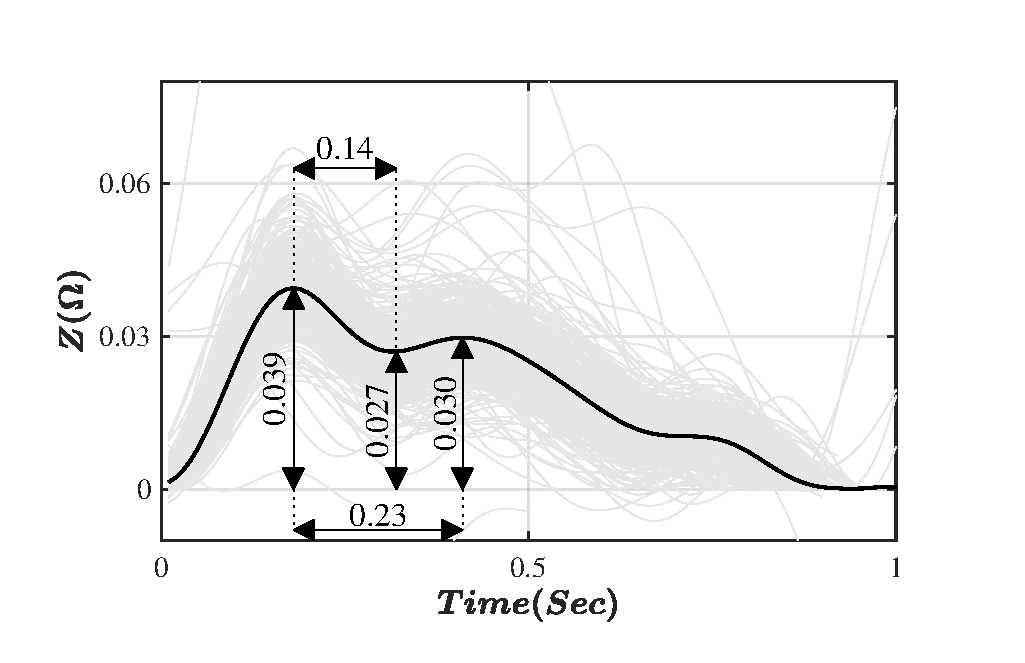
\includegraphics[width=0.48\textwidth, trim={0.5cm 0cm 1.5cm 0 cm}, clip]{figure_apa_4a}}%
	\hfill%
	\subcaptionbox{Average plethysmography waveform during venous occlusion region 4 (\SIrange{780}{960}{\second})\label{fig:iPG arterial occlusion}}
	[0.48\textwidth]{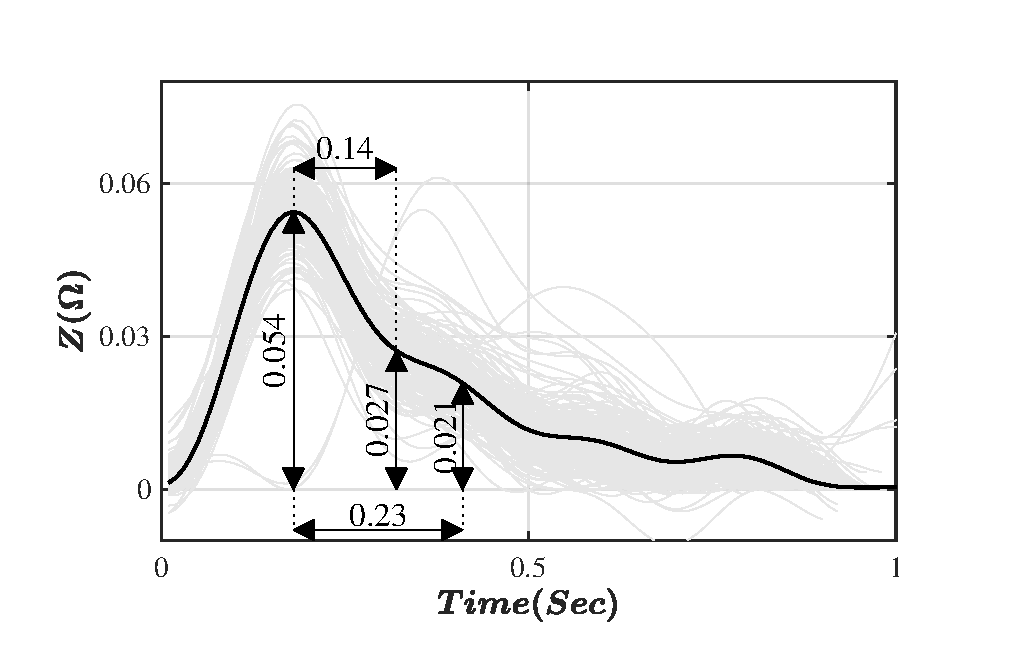
\includegraphics[width=0.48\textwidth, trim={0.5cm 0cm 1.5cm 0 cm}, clip]{figure_apa_4b}}%
	\hfill\null%
	\caption{Plethysmography waveform of the participant seven between baseline and partial arterial occlusion}
	\label{fig:iPG arterial}
	
	\vspace{1cm}
	
	\null\hfill%		
	\subcaptionbox{Change of amplitude of the waveform at point A.\label{fig:change A arterial}}
	[0.48\textwidth]{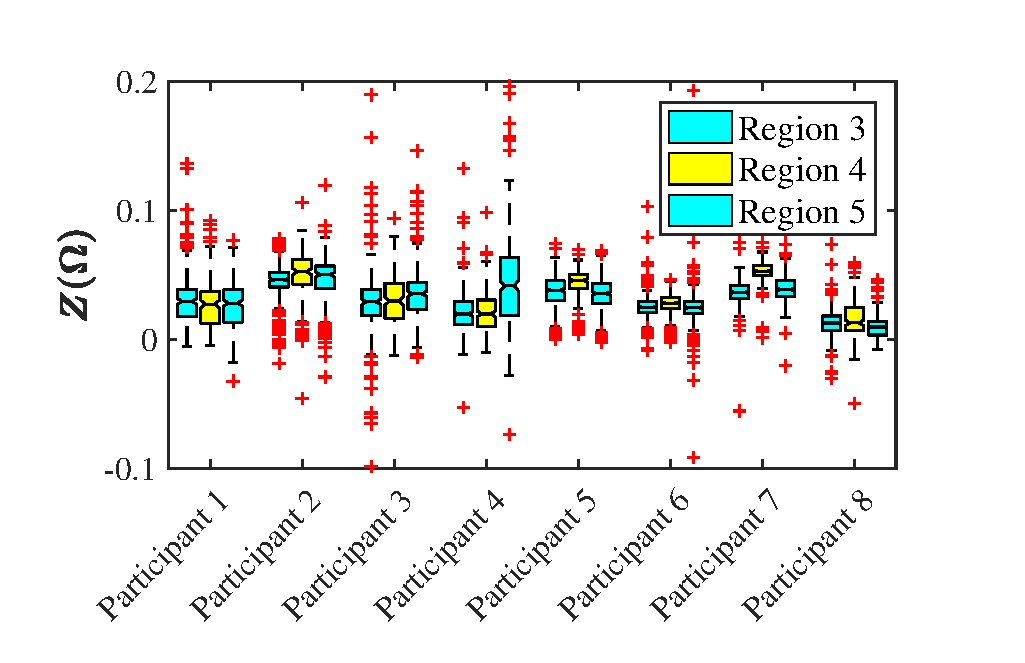
\includegraphics[width=0.48\textwidth, trim={0.5cm 0cm 1.5cm 0 cm}, clip]{figure_apa_5a}}%
	\hfill%
	\subcaptionbox{Change of amplitude of the waveform at point B.\label{fig:change B arterial}}
	[0.48\textwidth]{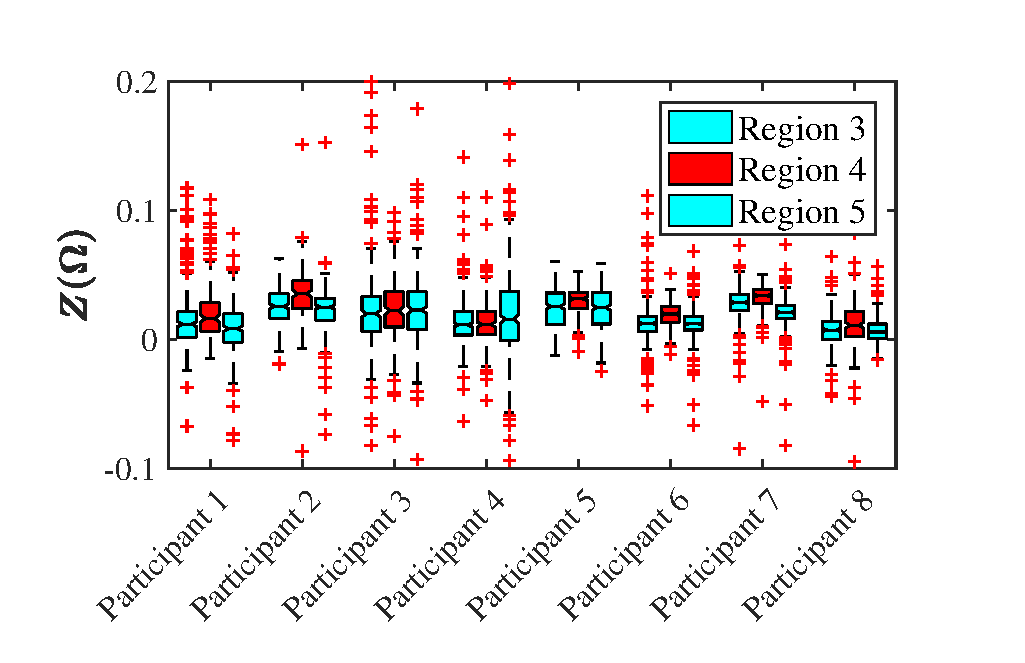
\includegraphics[width=0.48\textwidth, trim={0.5cm 0cm 1.5cm 0 cm}, clip]{figure_apa_5b}}%
	\hfill%
	\subcaptionbox{Change of amplitude of the waveform at point C.\label{fig:change C arterial}}
	[0.48\textwidth]{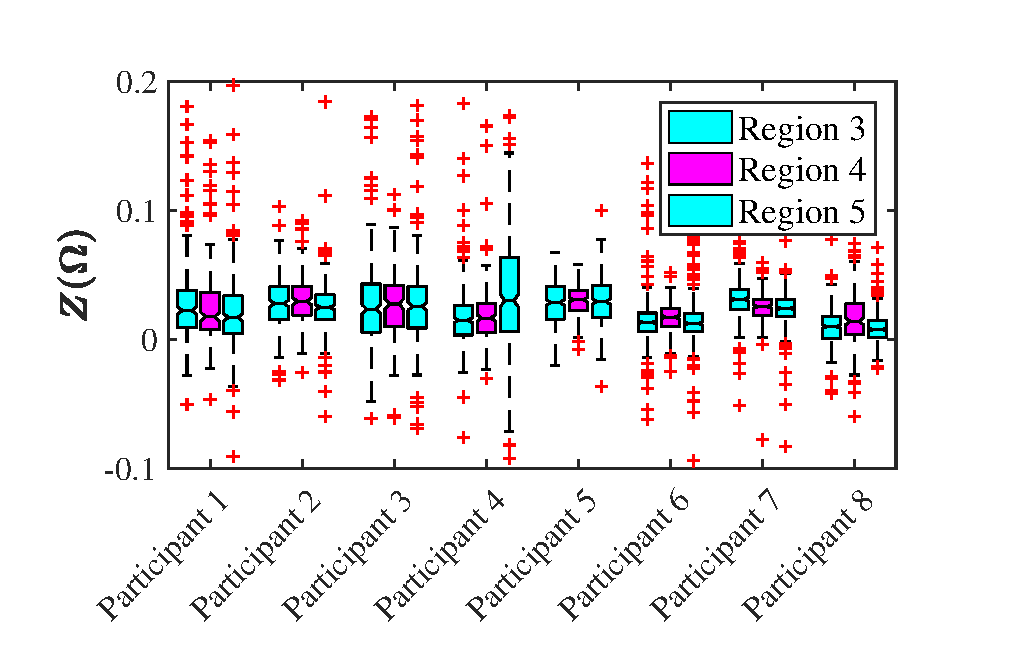
\includegraphics[width=0.48\textwidth, trim={0.5cm 0cm 1.5cm 0 cm}, clip]{figure_apa_5c}}%
	\null%
	\caption{Changes of the impedance peak values during baseline, partial arterial occlusion and return to baseline for points A,B and C.}
	\label{fig:iPG change points arterial}
\end{figure*}

\subsubsection{Changes in systolic peak (Point A)}
\label{section apa 3.2.1}
Figure \ref{fig:change A arterial} indicates the change in amplitude for each one of the participants. Also, table \ref{tbl:change A arterial} summarises the average impedances and the variations in each region. Through this occlusive experiment, 7 participants (\SI{87.5}{\percent}) displayed an increase in electrical resistivity at point A of about \SI{13.52}{\percent}. However, some of these participants showed a tiny increase in their peaks between \SIrange{0.29}{2.24}{\percent}. In general, one can note the hike at this point. After the cuff was deflated, most of the participants (\SI{62.5}{\percent}) showed a decrease of the peak in an average of \SI{-21.86}{\percent}.  In contrast, participants one, three and four registered an increase in their impedance reading, being the later an outlier with an increase in his magnitude of \SI{110.69}{\percent}.

\begin{table}[!htbp]
	\caption{Change of amplitude of the waveform at peak A during the transition from baseline to venous occlusion.}
	\label{tbl:change A arterial}
	\centering\small
	\begin{tabular}{l
					*{3}{S[table-format=1.4]@{\,\( \pm \)\,}S[table-format=1.4]} %Format for Z+-std
					>{\columncolor[gray]{0.8}}c>{\columncolor[gray]{0.9}}c}
		\toprule
		& \multicolumn{2}{c}{\multirow{2}{*}{\textbf{Baseline [\si{\ohm}]}}}
		& \multicolumn{2}{c}{\multirow{2}{*}{\textbf{Occlusion [\si{\ohm}]}}}
		& \multicolumn{2}{c}{\multirow{2}{*}{\textbf{Baseline [\si{\ohm}]}}}
		& \multicolumn{2}{c}{\textbf{Change}} \\
		& \multicolumn{2}{c}{}
		& \multicolumn{2}{c}{}
		& \multicolumn{2}{c}{}
		&\textbf{R3-R4}&\textbf{R4-R5}\\\midrule
	    Participant 1 & 0.0295 & 0.0194 & 0.0274 & 0.0190 & 0.0282 & 0.0265 & -7.03 \% &   2.59 \% \\  
		Participant 2 & 0.0462 & 0.0140 & 0.0526 & 0.0197 & 0.0503 & 0.0461 & 13.78 \% &  -5.11 \% \\  
		Participant 3 & 0.0292 & 0.0379 & 0.0298 & 0.0185 & 0.0354 & 0.0356 &  2.24 \% &  19.02 \% \\  
		Participant 4 & 0.0197 & 0.0242 & 0.0198 & 0.0152 & 0.0416 & 0.0453 &  0.29 \% & 110.69 \% \\  
		Participant 5 & 0.0382 & 0.0133 & 0.0458 & 0.0115 & 0.0357 & 0.0351 & 19.81 \% & -26.55 \% \\  
		Participant 6 & 0.0249 & 0.0096 & 0.0282 & 0.0081 & 0.0247 & 0.0251 & 13.21 \% & -14.09 \% \\  
		Participant 7 & 0.0365 & 0.0097 & 0.0529 & 0.0092 & 0.0388 & 0.0394 & 44.90 \% & -38.73 \% \\  
		Participant 8 & 0.0128 & 0.0104 & 0.0128 & 0.0160 & 0.0096 & 0.0098 &  0.38 \% & -24.86 \% \\      
		\bottomrule
	\end{tabular} 
\end{table}\subsubsection{Changes in dicrotic notch peak (Point B)}
\label{section apa 3.2.2}
In the dicrotic notch position (point B), the increase of its magnitude is clearer than in the systolic peak. In fact, all the participants depicted an increase in their impedance value at this point. Figure \ref{fig:change B arterial} evidence these shifts in each of the regions before and after the occlusion. Table \ref{fig:change B arterial} details participants' median impedances and the ratio of change in each region.

In general, the average increase at the dicrotic notch as soon as the occlusion was applied was about \SI{29.91}{\percent}. When the pressure restricting the blood flow was removed, six out of eight of the study members experienced a fall in electrical resistivity towards baseline. On average, it reduced by \SI{-51.72}{\percent}. Again, participant four was the exception to this reduction, as well as participant three. Their impedance rose by \SI{37.37}{\percent} and \SI{3.25}{\percent} respectively.

\begin{table}[!htbp]
	\caption{Change of amplitude of the waveform at peak B during the transition from baseline to venous occlusion.}
	\label{tbl:change B arterial}
	\centering\small
	\begin{tabular}{l
					*{3}{S[table-format=1.4]@{\,\( \pm \)\,}S[table-format=1.4]} %Format for Z+-std
					>{\columncolor[gray]{0.8}}c>{\columncolor[gray]{0.9}}c}
		\toprule
		& \multicolumn{2}{c}{\multirow{2}{*}{\textbf{Baseline [\si{\ohm}]}}}
		& \multicolumn{2}{c}{\multirow{2}{*}{\textbf{Occlusion [\si{\ohm}]}}}
		& \multicolumn{2}{c}{\multirow{2}{*}{\textbf{Baseline [\si{\ohm}]}}}
		& \multicolumn{2}{c}{\textbf{Change}} \\
		& \multicolumn{2}{c}{}
		& \multicolumn{2}{c}{}
		& \multicolumn{2}{c}{}
		&\textbf{R3-R4}&\textbf{R4-R5}\\\midrule
		Participant 1 & 0.0119 & 0.0232 & 0.0162 & 0.0220 & 0.0083 & 0.0087 & 36.07 \% & -66.02 \% \\  
		Participant 2 & 0.0257 & 0.0142 & 0.0354 & 0.0212 & 0.0251 & 0.0231 & 38.02 \% & -40.44 \% \\  
		Participant 3 & 0.0200 & 0.0536 & 0.0222 & 0.0247 & 0.0229 & 0.0244 & 11.33 \% &   3.25 \% \\  
		Participant 4 & 0.0113 & 0.0256 & 0.0116 & 0.0177 & 0.0158 & 0.0143 &  2.64 \% &  37.37 \% \\  
		Participant 5 & 0.0254 & 0.0155 & 0.0314 & 0.0107 & 0.0248 & 0.0237 & 23.55 \% & -26.29 \% \\  
		Participant 6 & 0.0124 & 0.0150 & 0.0197 & 0.0096 & 0.0121 & 0.0141 & 58.95 \% & -61.59 \% \\  
		Participant 7 & 0.0287 & 0.0128 & 0.0340 & 0.0104 & 0.0211 & 0.0205 & 18.34 \% & -44.99 \% \\  
		Participant 8 & 0.0073 & 0.0118 & 0.0110 & 0.0196 & 0.0058 & 0.0069 & 50.41 \% & -71.01 \% \\      
\bottomrule
	\end{tabular} 
\end{table}

\subsubsection{Changes in diastolic peak (Point C)}
\label{section apa 3.2.3}
Changes in the diastolic peak also presented a similar increasing trend as seen in points A and B. However; the changes were not as marked as the ones seen in the dicrotic notch. Figure \ref{fig:change C arterial} and Table \ref{tbl:change C arterial} summarise the values obtained. In total, \SI{75}{\percent} of the participants showed an increase of impedance between region 3 and 4. It increased with a median of \SI{18.74}{\percent}. Participant eight showed a change significantly larger than the mean (\SI{44.11}{\percent}). Study members one and seven pointed a decrease of electrical resistivity in \SI{-19.91}{\percent} on average.  

On the opposite side of the exercise, after releasing the pressure, (\SI{87.5}{\percent}) of the partakers showed a reduction in their impedance, including those whose impedance rose during the occlusion. On average, impedance reduced by \SI{-19.77}{\percent} in total. Again, participant four showed an increase in the ratio of change before and after the blockage significantly exceeding the median of all the measurements. Moreover, this study member outperformed notably the average ratio after the occlusion (\SI{90.32}{\percent}). As portrayed by the other measuring points, this confirms that the data obtained from this study member were not from physiological origin but motion or randomness. 

\begin{table}[!htbp]
	\caption{Change of amplitude of the waveform at peak C during the transition from baseline to venous occlusion.}
	\label{tbl:change C arterial}
	\centering\small
	\begin{tabular}{l
					*{3}{S[table-format=1.4]@{\,\( \pm \)\,}S[table-format=1.4]} %Format for Z+-std
					>{\columncolor[gray]{0.8}}c>{\columncolor[gray]{0.9}}c}
		\toprule
		& \multicolumn{2}{c}{\multirow{2}{*}{\textbf{Baseline [\si{\ohm}]}}}
		& \multicolumn{2}{c}{\multirow{2}{*}{\textbf{Occlusion [\si{\ohm}]}}}
		& \multicolumn{2}{c}{\multirow{2}{*}{\textbf{Baseline [\si{\ohm}]}}}
		& \multicolumn{2}{c}{\textbf{Change}} \\
		& \multicolumn{2}{c}{}
		& \multicolumn{2}{c}{}
		& \multicolumn{2}{c}{}
		&\textbf{R3-R4}&\textbf{R4-R5}\\\midrule
	    Participant 1 & 0.0224 & 0.0323 & 0.0176 & 0.0307 & 0.0171 & 0.0206 & -21.35 \% &  -2.21 \% \\  
		Participant 2 & 0.0279 & 0.0196 & 0.0295 & 0.0272 & 0.0250 & 0.0252 &   5.96 \% & -16.45 \% \\  
		Participant 3 & 0.0236 & 0.0826 & 0.0275 & 0.0284 & 0.0256 & 0.0283 &  16.56 \% &  -7.98 \% \\  
		Participant 4 & 0.0149 & 0.0327 & 0.0166 & 0.0229 & 0.0301 & 0.0306 &  11.22 \% &  90.32 \% \\  
		Participant 5 & 0.0287 & 0.0171 & 0.0308 & 0.0119 & 0.0293 & 0.0287 &   7.32 \% &  -5.03 \% \\  
		Participant 6 & 0.0133 & 0.0252 & 0.0174 & 0.0111 & 0.0123 & 0.0176 &  30.32 \% & -37.72 \% \\  
		Participant 7 & 0.0312 & 0.0189 & 0.0254 & 0.0124 & 0.0241 & 0.0232 & -18.48 \% &  -4.27 \% \\  
		Participant 8 & 0.0100 & 0.0139 & 0.0141 & 0.0224 & 0.0076 & 0.0087 &  41.11 \% & -64.75 \% \\  
		\bottomrule
	\end{tabular} 
\end{table}

\subsection{Plethysmography waveform change during total occlusion}
\label{section apa 3.3}
Performing total occlusion completely blocks the inflow and outflow of blood beneath the arm's cuff.  Hence, there is no change of volume within the arm's segment. As a result, impedance plethysmography should not present changes.  Figure \ref{fig:iPG_total} shows the plethysmography baseline in region 5 (\SIrange{960}{1260}{\second}) and region 6  (\SIrange{1260}{1440}{\second}) of participant seven. As portrayed by Figure \ref{fig:iPG_change_points_total}, the amplitudes of most of the participants dropped during the occlusion.

However, participant four experienced different behaviour in all these points. The standard deviation of this participant also suggests that there would have been a problem with his plethysmography signal during the test. 

In general, point A decreased on average by \SI{-66.15}{\percent} at its peak value occlusion. Then when the pressure was released, impedance recovered its value in \SI{75.98}{\percent}. A similar event occurred with point B; peak signals dropped a median of \SI{-63.29}{\percent} during blockage and recovered on average by \SI{74.02}{\percent}. Similarly, point C, decreased on average by \SI{-50.27}{\percent}  and increased by \SI{58.71}{\percent} after the occlusion.

%This method allows multifigures being aligned using subcaptionbox
\begin{figure*}
	\centering
	\null\hfill%
	\subcaptionbox{Average plethysmography waveform during venous occlusion region 5 (\SIrange{960}{1260}{\second})\label{fig:iPG_total_baseline}}
	[0.48\textwidth]{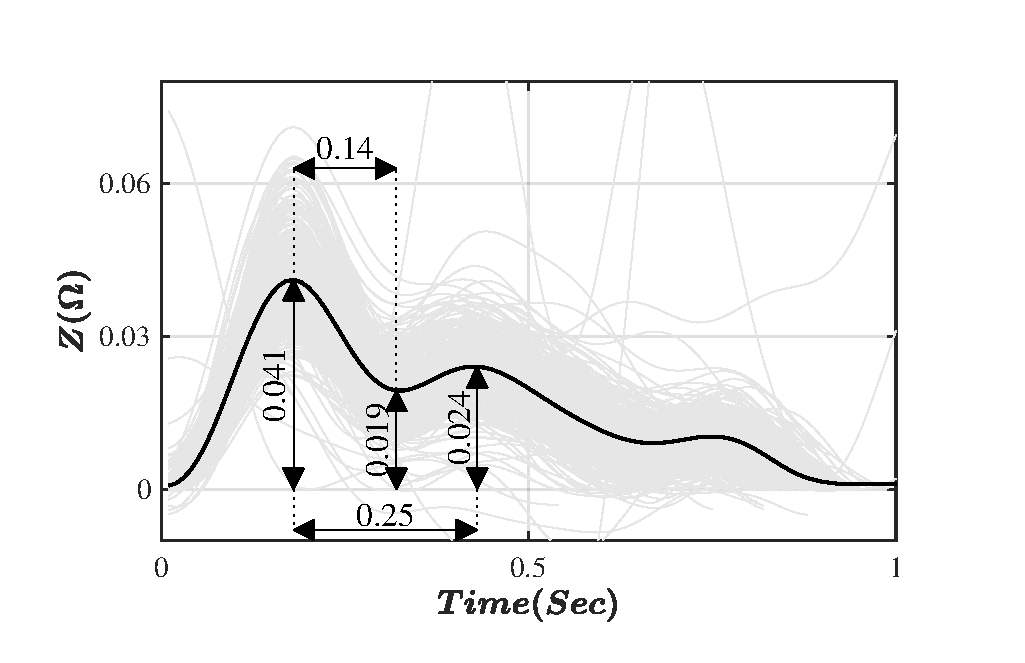
\includegraphics[width=0.48\textwidth, trim={0.5cm 0cm 1.5cm 0 cm}, clip]{figure_apa_6a}}%
	\hfill%
	\subcaptionbox{Average plethysmography waveform during venous occlusion region 6 (\SIrange{1260}{1440}{\second})\label{fig:iPG_total_occlusion}}
	[0.48\textwidth]{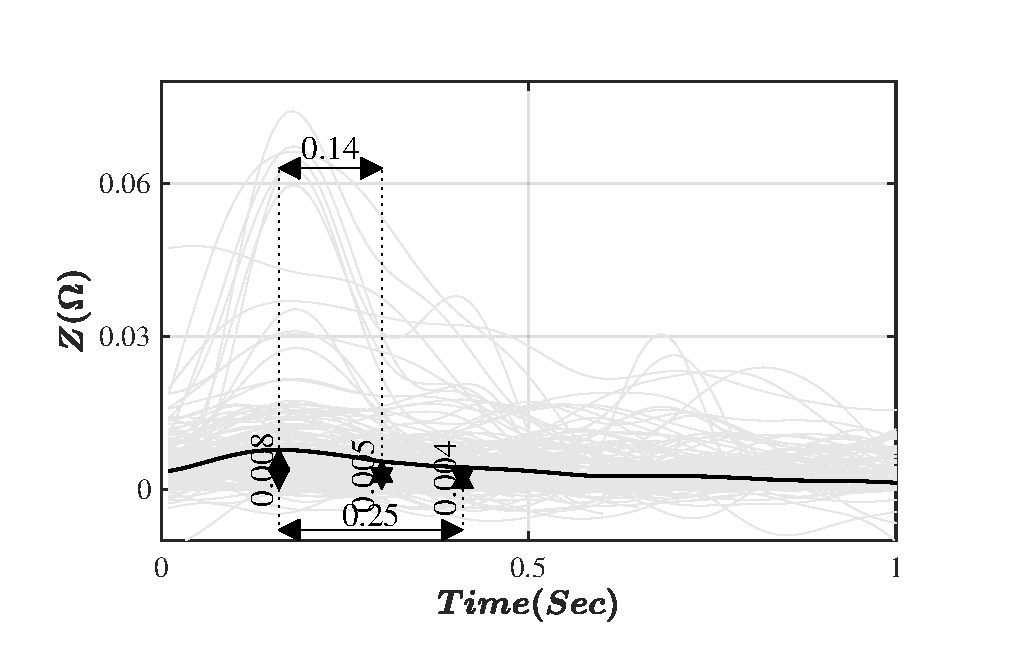
\includegraphics[width=0.48\textwidth, trim={0.5cm 0cm 1.5cm 0 cm}, clip]{figure_apa_6b}}%
	\hfill\null%
	\caption{Plethysmography waveform of the participant seven between baseline and total occlusion}
	\label{fig:iPG_total}
	
	\vspace{1cm}
	
	\null\hfill%		
	\subcaptionbox{Change of amplitude of the waveform at point A.\label{fig:change_A_total}}
	[0.48\textwidth]{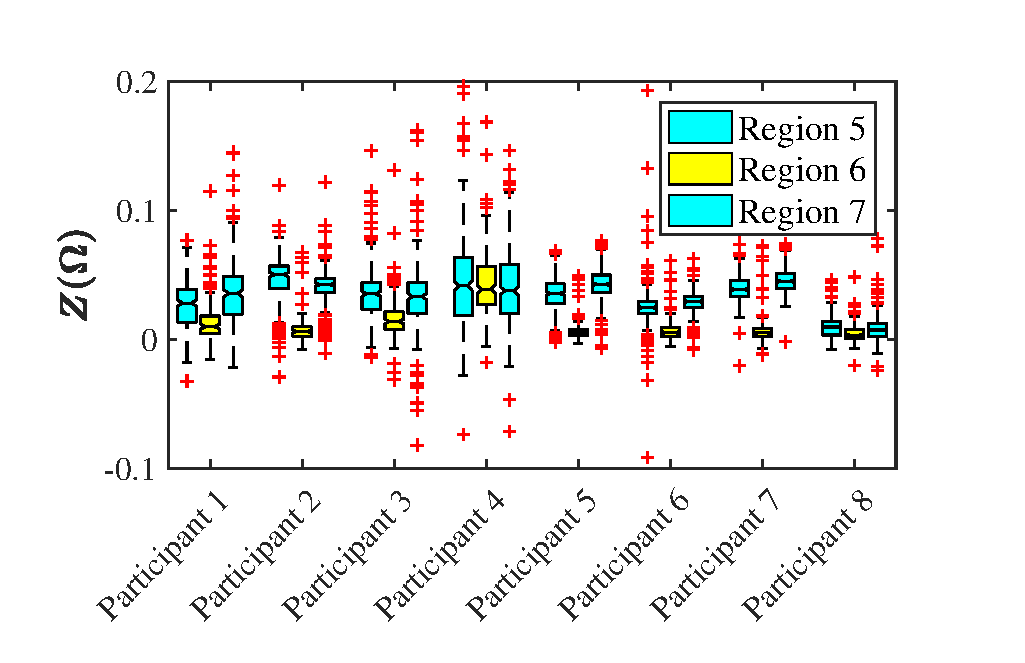
\includegraphics[width=0.48\textwidth, trim={0.5cm 0cm 1.5cm 0 cm}, clip]{figure_apa_7a}}%
	\hfill%
	\subcaptionbox{Change of amplitude of the waveform at point B.\label{fig:change_B_total}}
	[0.48\textwidth]{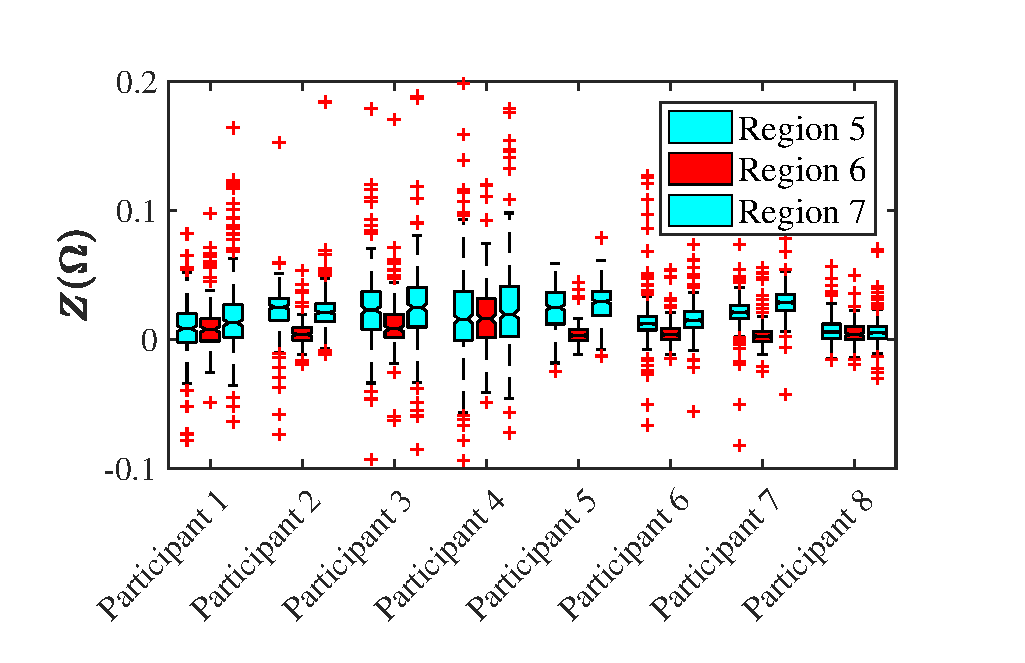
\includegraphics[width=0.48\textwidth, trim={0.5cm 0cm 1.5cm 0 cm}, clip]{figure_apa_7b}}%
	\hfill%
	\subcaptionbox{Change of amplitude of the waveform at point C.\label{fig:change_C_total}}
	[0.48\textwidth]{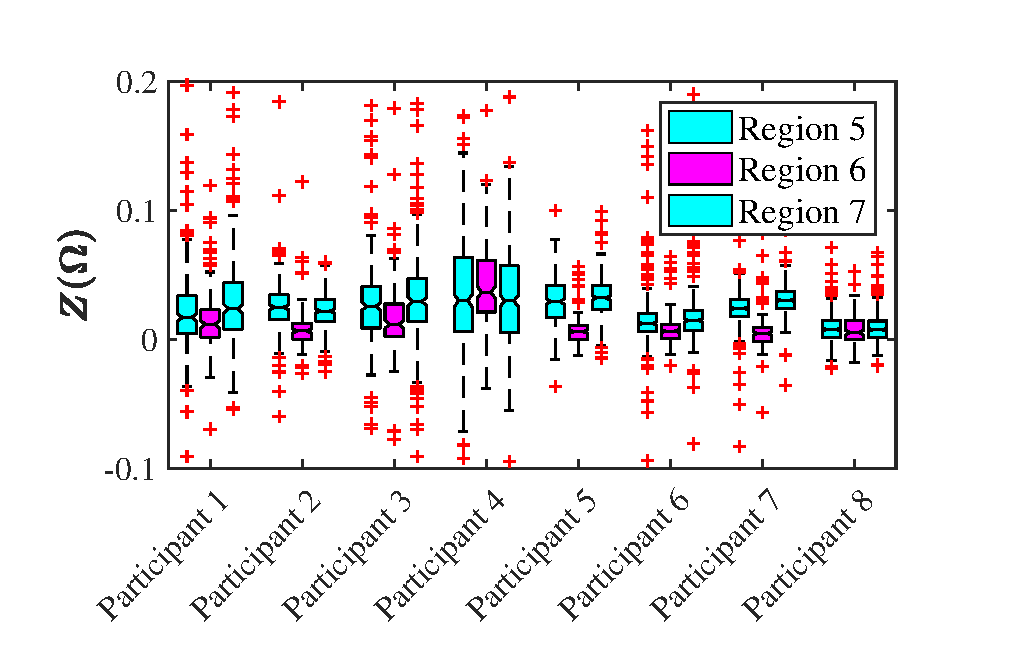
\includegraphics[width=0.48\textwidth, trim={0.5cm 0cm 1.5cm 0 cm}, clip]{figure_apa_7c}}%
	\null%
	\caption{Changes of the impedance peak values during baseline, total occlusion and return to baseline for points A,B and C.}
	\label{fig:iPG_change_points_total}
\end{figure*}

%%********************************** % Section 5.5 ******************************************
\section{Blood flow calculation from plethysmography signal}
\label{section apa 5}
So far the blood flow has been analysed from occlusive methods using the techniques described in section \ref{section apa 4}. However, these procedures require mechanical occlusion to produce an increase in volume within the forearm being measured. Nevertheless, sometimes this can be uncomfortable, especially when the applied pressure is above the systolic value or when the person simply can not tolerate restriction of blood flow.

For these cases, analysing the waveform also provides information about the blood flow.  The rush of blood into the vessel creates a small increase in volume within the limit of the potential electrodes which can be translated into a quantifiable blood flow. Having a device sensitive enough to detect these changes is crucial to provide an accurate estimation of the blood speed. As described in section \ref{section apa 3}, the waveform contained within the basal impedance was amplified by the device, achieving great detail. 

In fact, several studies \mynote{Add a reference to a study about AC blood flow estimation} have demonstrated that it is possible to calculate blood flow from the plethysmography waveform. In this case, the change of impedance used to perform this calculation occurs between the foot of the wave and the systolic peak. This $\Delta Z$ is used to calculate blood flow by also applying Nyober's equation \ref{eq:Nyober}. 

Figure \ref{fig:blood_flow_plethysmography} demonstrates the blood flow calculated from the amplitude of the systolic peak throughout the experimental session. Green dots show blood flow measurements during reference readings (regions 1, 3, 5 and 6). The other colours show venous occlusion in blue, partial arterial occlusion in red and total obstruction in grey. The dark line drawn above the signals corresponds to the calculation of the sixth-order polynomial fit during each measurement event. Overseeing the amplitude transition in each region will help explain how the flow changes with each occlusive event. The blood flow shown in the same figure does not include the negative sign which represents the direction of flow relative to the potential electrodes.

\begin{figure}[!htb]
	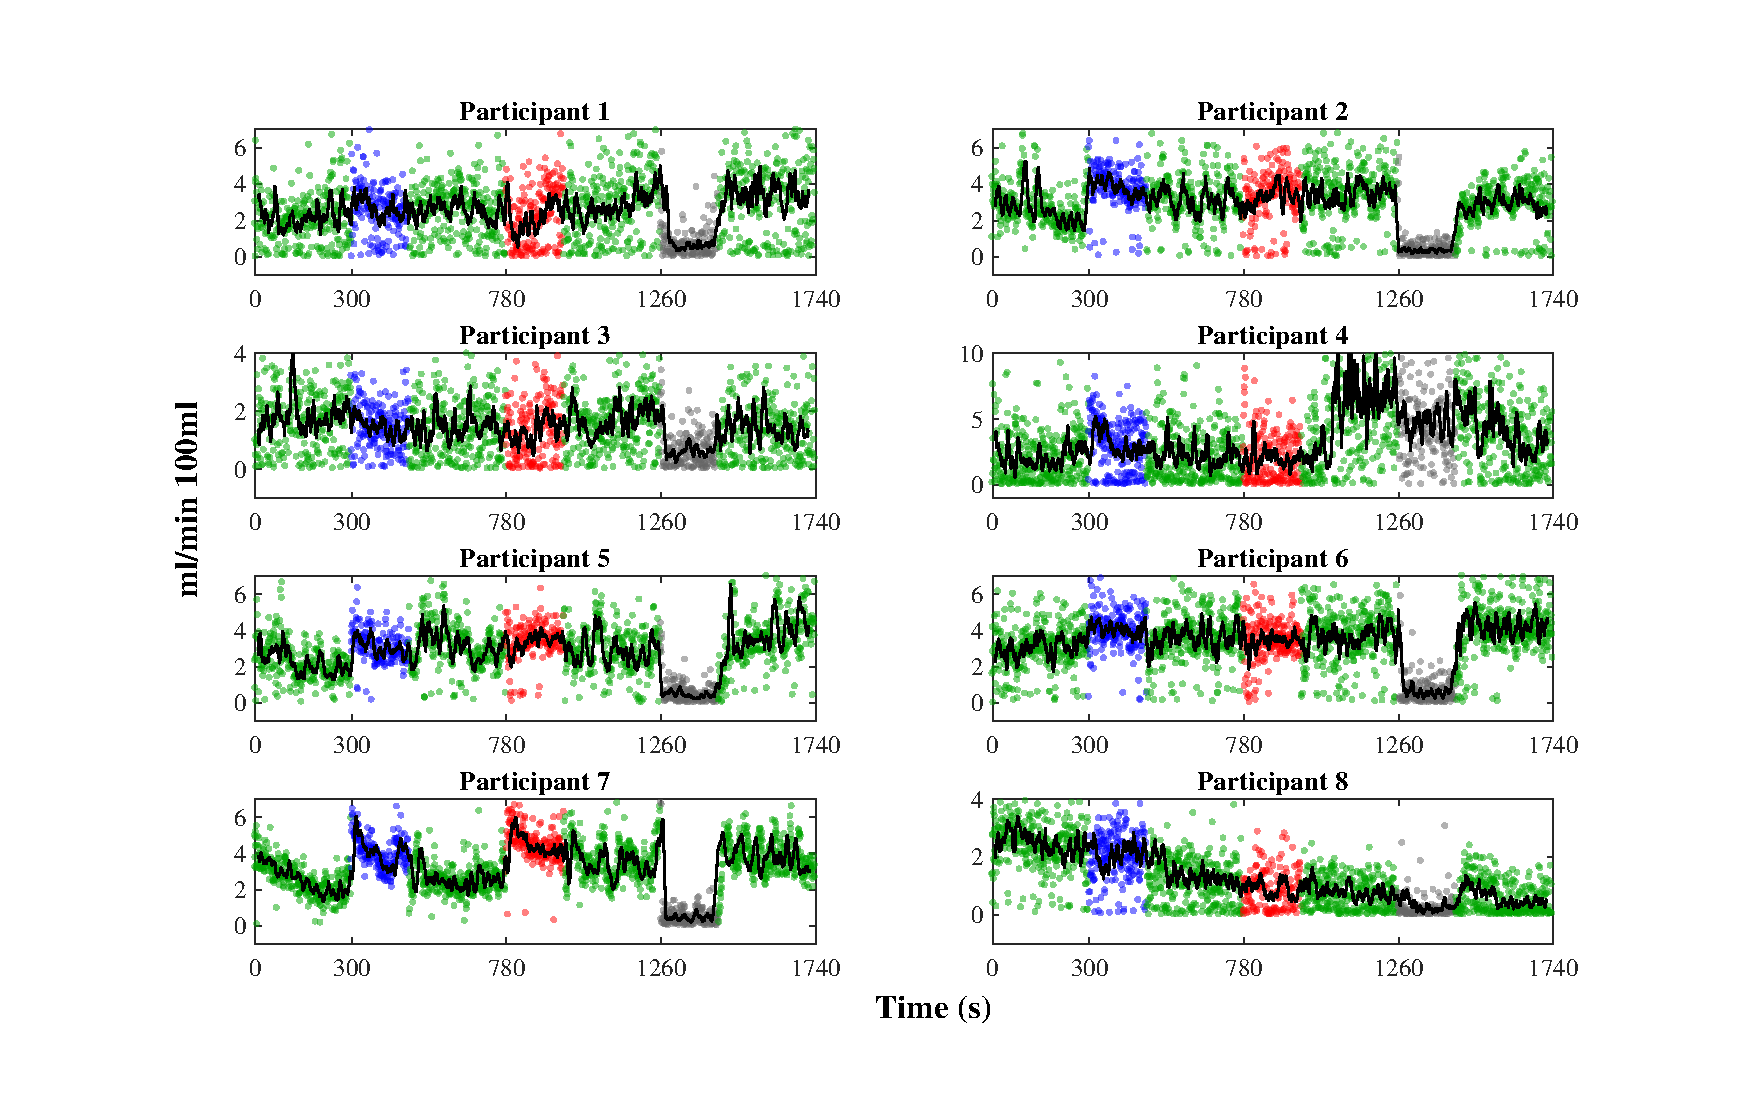
\includegraphics[width=\textwidth,keepaspectratio,trim={3cm 0cm 3cm 0 cm},clip]{figure15}    
	\caption[Blood flow calculated from impedance plethysmography waveform at the time of the whole expetiment]{Blood flow calculated for all the participants during the experiment. Each dot represents the peak value of the waveform that has been converted into flow (\si{\bfv}). The green dotted area represent the baselines measurements (regions 1,3,5 and 7). The region 2 (venous occlusion) is represented by the blue dots, arterial occlusions (region 4) are in red and total occlusions (region 6) are in grey.}
	\label{fig:blood_flow_plethysmography}
\end{figure}

As portrayed in the figure, between each transition, in the middle of baseline and occlusion, there is a change in the calculated flow. In most participants, the change between baseline and venous occlusion creates a blood surge followed by a tendency for the flow to stabilise. It is worth noting that the addition of blood flow in participant 2 occurred before the occlusion. The reason for this is that the obstruction probably started before \SI{300}{\second} and the pressure applied to the arm was rather slow. There are other cases where the flow change occurred so fast that an entirely blank space can be seen connecting both events, as in participants 5 and 7. This situation, as opposed to participant 2, was more likely due to the cuff being inflated faster which did not allow a gradual but instead sudden change in flow. Finally, participant 8 is an exception to this rule. This participant experienced a decrease in flow, followed by a recovery and, he did not show a flow surge.

Between venous occlusion and baseline in region 3, the cuff was rapidly deflated to return blood flow to normal. However, from the calculated data it can be seen that there are no extreme changes in blood flow between these two sections. As noted, in most participants except partaker 1, there are small gaps between these two sections indicating that there is a slight change in blood flow. This action can be linked to a hyperaemic effect where as soon as the pressure of the cuff is released, the blood contained within the vessels of the forearm runs out to the upper part of the arm. After that, the blood flow tended to stabilise towards an average value. 

Similarly, as between regions 1 and 2, the change between baseline (region 3) and partial arterial occlusion (region 4) generated alterations in the calculated blood flow. Some participants also showed a rapid increase in blood flow followed by settling in the blood velocity. The only ones that did not enact a similar behaviour were participants 2 and 8. However, partaker 7 appears to be Gaussian bell-shaped flow, which seems to indicate that the occlusion did not occur at the right moment but rather a little while later. Interestingly, the figure also shows that blood flow did not fully stabilise in participants 1, 3 and 8.

The change between partial arterial occlusion and baseline had a similar effect as the one described for the release of pressure of venous blockage. Most of the participants showed a decrease in their blood flow, possibly caused by the hyperaemic effect. At this point one can note that participant 4 started to show random blood flow readings. 

Total occlusion had a response as expected in almost all participants. When the blood flow was completely stopped, it was anticipated that its calculated value could tend to zero. In this case, the device was able to detect these changes. The only exception was participant 4 who again showed random results. At this point, it was to be expected that something wrong was happening with his measurements. Then, when the tourniquet was released, the blood flow returned in an exponential form and then set to an average value. In this case, the hyperaemic effect is more visible. It is worth noting that participant 8 showed a decline in blood flow measurements towards the midpoint of the test. This event agrees, with the participant expressing not feeling very well at the end of the test. One can speculate it being a coincidence, or maybe the device was able to detect these physiological changes in him.

It seems evident that there is a blood surge when an occlusion occurs. Subsequently, the blood flow tends to stabilise at an average value. When the blockage is released, it seems that in some cases the flow tends to decrease and in others, there is no apparent change. The following sections will show the results of the change in mean blood flow during each occlusive event.


%********************************** % Section 5.5.1 ******************************************
\subsection{Blood flow change during venous occlusion}
\label{sectio results 5.1}
The following are the results of calculating mean blood flow between the transitions of baseline, venous occlusion and return to the reference signal. Once again, the result of the calculation is the absolute value, dropping the negative sign. Table \ref{tbl:blood_flow_iPG_venous} shows the result obtained by flow measurement in scale \si{\bfv}. The mean blood flow in region 1 was about \SI{2.398(0378)}{\bfv}. When the cuff was inflated below diastolic value, the blood flow calculated in region 2, there was an average blood flow step-up of about \SI{3.043(0378)}{\bfv} \nknote{?}. It is easy to see that in general terms there was an increment in the blood flow during the occlusion. In fact, \SI{75}{\percent} of the participants experienced this increment of blood flow. Only, study members 3 and 8 showed a decrease in their blood flow during this transition. The latter is not a surprise, as it was noted before, all his recordings started to go downwards from the beginning of the test. Their \nknote{who?} blood flow decreased in average roughly \SI{0.356(0023)}{\bfv}.

Clearly, there is a blood flow decrement\nknote{decrement??} when the cuff's tension was released to return to baseline. Indeed, seven out of eight of the participants experienced a drop in their flow rate during this part of the experiment. The average blood flow for region 3 was approximately \SI{2.459(0852)}{\bfv}. The only one who did not experience this change was participant 6 whose flow rate dropped \SI{-0.0101}{\bfv} which means that there was practically no change. 

\begin{table}[h]
	\caption{Mean blood flow calculated form the plethysmography wave for baseline, venous occlusion and return to baseline}
	\label{tbl:blood_flow_iPG_venous}
	\centering
	\begin{tabular}{l
				    *{3}{S[table-format=1.3]@{\,\( \pm \)\,}S[table-format=1.3]} %Format for Z+-std
					}
		\toprule
		& \multicolumn{2}{c}{\textbf{Region 1}}
		& \multicolumn{2}{c}{\textbf{Region 2}} 
		& \multicolumn{2}{c}{\textbf{Region 3}}  \\
		& \multicolumn{2}{c}{\small{\si{[\bfv]}}} 
		& \multicolumn{2}{c}{\small{\si{[\bfv]}}} 
		& \multicolumn{2}{c}{\small{\si{[\bfv]}}} \\\midrule
		Participant 1    &     2.206     &     1.772    &     2.695     &     1.638    &     2.528     &     1.481    \\  
		Participant 2    &     2.715     &     1.185    &     3.786     &     1.161    &     3.122     &     1.252    \\  
		Participant 3    &     1.809     &     1.282    &     1.469     &     0.796    &     1.376     &     1.260    \\  
		Participant 4    &     2.178     &     2.032    &     3.088     &     2.010    &     2.177     &     1.959    \\  
		Participant 5    &     2.227     &     1.082    &     3.132     &     0.947    &     3.142     &     1.277    \\  
		Participant 6    &     3.035     &     1.289    &     4.049     &     1.146    &     3.581     &     1.330    \\  
		Participant 7    &     2.579     &     0.930    &     4.057     &     0.924    &     2.567     &     0.827    \\  
		Participant 8    &     2.437     &     0.874    &     2.065     &     0.901    &     1.176     &     0.729    \\  
		\bottomrule
	\end{tabular}
\end{table}

%********************************** % Section 5.5.2 ******************************************
\subsection{Blood flow change during partial arterial occlusion}
\label{section apa 5.2}
The change of blood flow between baseline and partial occlusion had not a common ?? in all the study participants response as the one seen in the previous section. Their flow rate increased from an average of \SI{2.458(0852)}{\bfv} to a mean blood flow of \SI{2.649(1200)}{\bfv}. It is clear that the increase was not as notorious compared to that seen on the venous occlusion. Indeed, only three participants (2, 5 and 7) showed an increment in blood flow with a centre of \SI{0.774(0983)}{\bfv}. Participant 3 showed a particularly higher increase in blood flow than the others with a value of \SI{1.099}{\bfv}. Conversely, the rest of the participants exhibited a small decrease in their blood flow with an average of \SI{-0.160(0101)}{\bfv}. 

When the upper arm pressure was released, most participants were expected to show a decline in their flow. However, this was not the case. Clearly, three participants depicted a drop in the rate (5, 7 and 8 with an average of \SI{-0.541(0371)}{\bfv}). The rest of the study members showed an increase in their collected data. Notwithstanding, as previously described in this region, participant 4 showed random values whose results will therefore not be added up to the total mean in the following calculation. The midpoint increase in blood flow between the others was \SI{0.329(0205)}{\bfv}. At this stage, it is not possible to draw a clear conclusion of the change of blood flow when the arterial occlusion occurred. 

\begin{table}[h]
	\caption{Mean blood flow calculated form the plethysmography wave for baseline, partial arterial occlusion and return to baseline}
	\label{tbl:blood_flow_iPG_arterial}
	\centering
	\begin{tabular}{l
			*{3}{S[table-format=1.3]@{\,\( \pm \)\,}S[table-format=1.3]} %Format for Z+-std
		}
		\toprule
		& \multicolumn{2}{c}{\textbf{Region 3}}
		& \multicolumn{2}{c}{\textbf{Region 4}} 
		& \multicolumn{2}{c}{\textbf{Region 5}}  \\
		& \multicolumn{2}{c}{\small{\si{[\bfv]}}} 
		& \multicolumn{2}{c}{\small{\si{[\bfv]}}} 
		& \multicolumn{2}{c}{\small{\si{[\bfv]}}} \\\midrule
		Participant 1    &     2.528     &     1.481    &     2.255     &     1.689    &     2.853     &     1.791    \\  
		Participant 2    &     3.122     &     1.252    &     3.298     &     1.399    &     3.418     &     1.492    \\  
		Participant 3    &     1.376     &     1.260    &     1.336     &     1.025    &     1.700     &     1.132    \\  
		Participant 4    &     2.177     &     1.959    &     2.091     &     1.895    &     5.669     &     7.032    \\  
		Participant 5    &     3.142     &     1.277    &     3.380     &     0.994    &     2.885     &     1.225    \\  
		Participant 6    &     3.581     &     1.330    &     3.432     &     1.197    &     3.667     &     1.558    \\  
		Participant 7    &     2.567     &     0.827    &     4.476     &     1.001    &     3.543     &     1.050    \\  
		Participant 8    &     1.176     &     0.729    &     0.924     &     0.864    &     0.729     &     0.537    \\  
	\bottomrule
	\end{tabular}
\end{table}

%********************************** % Section 5.5.3 ******************************************
\subsection{Blood flow change during total occlusion}
\label{section apa 5.3}
The results obtained from total occlusion were quite close to the expected values.  The majority of the study participants showed a decrease in blood circulation rate close to zero.  As is evident from table \ref{tbl:blood_flow_iPG_total}, almost all participants showed a large drop in the blood flow measurement when the blockage was applied in region 6. Once more, Participant 4 displayed a completely unusual response during the occlusion. The values obtained were on average \SI{0.599(0224)}{\bfv} discarding data from partaker 4 \nknote{do you mean to staop and make this a new sentence or what?}. Clearly, the flow obtained did not reflect a zero blood flow. The calculated values correspond to the amplitude of the noise level captured by the device. 

\begin{table}[!htbp]
	\caption{Mean blood flow calculated form the plethysmography wave for baseline, total occlusion and return to normality}
	\label{tbl:blood_flow_iPG_total}
	\centering
	\begin{tabular}{l
			*{3}{S[table-format=1.3]@{\,\( \pm \)\,}S[table-format=1.3]} %Format for Z+-std
		}
		\toprule
		& \multicolumn{2}{c}{\textbf{Region 5}}
		& \multicolumn{2}{c}{\textbf{Region 6}} 
		& \multicolumn{2}{c}{\textbf{Region 7}}  \\
		& \multicolumn{2}{c}{\small{\si{[\bfv]}}} 
		& \multicolumn{2}{c}{\small{\si{[\bfv]}}} 
		& \multicolumn{2}{c}{\small{\si{[\bfv]}}} \\\midrule
		Participant 1    &     2.853     &     1.791    &     0.908     &     1.283    &     3.407     &     2.553    \\  
		Participant 2    &     3.418     &     1.492    &     0.448     &     0.698    &     2.833     &     1.179    \\  
		Participant 3    &     1.700     &     1.132    &     0.704     &     0.751    &     1.387     &     1.210    \\  
		Participant 4    &     5.669     &     7.032    &     4.657     &     2.868    &     3.829     &     4.128    \\  
		Participant 5    &     2.885     &     1.225    &     0.560     &     0.687    &     3.619     &     1.645    \\  
		Participant 6    &     3.667     &     1.558    &     0.759     &     1.190    &     4.086     &     1.489    \\  
		Participant 7    &     3.543     &     1.050    &     0.597     &     1.121    &     3.767     &     0.958    \\  
		Participant 8    &     0.729     &     0.537    &     0.218     &     0.449    &     0.592     &     0.567    \\  
		\bottomrule
	\end{tabular}
\end{table}

After the tourniquet had been withdrawn, the blood flow returned to baseline following an exponential shape \nknote{what shape?? do want another word?} in most of the participants as shown in figure \ref{fig:blood_flow_plethysmography}. The mean blood flow in the region 7 was about \SI{2.940(1276)}{\bfv}. However, it can be seen that participant 8 had an expected drop in the flow rate before the blockage and then an increase in value. This event is fascinating as these changes occurred in a blood flow bellow \SI{1}{\bfv} but the device was able to notice the swing of blood flow rate. At this stage, the sensitivity for calculation of small changes in blood flow needs improvement because it detected flow values in other participants when there was no plethysmography signal. However, it is quite remarkable to see that the instrument is capable of detecting changes in the trend.

%%********************************** % Section 5.10 ******************************************
\section{Conclusions}
\label{section apa 10}
All the signals recorded were clear and offered an overview of what could happen during each occlusive event. The designed impedance device demonstrated that it was able to detect changes in basal impedance and plethysmography signals. Moreover, it seems that each occlusive event manifests a particular response like slope change in basal impedance and waveform amplitude at systolic and diastolic peaks during occlusions. \nknote{change this last sentence}

The other instruments were also able to detect changes during each event. For instance, the ultrasound device, referencing arterial flow, detected changes mostly in region 4 and 6 of the study. The LDF pointing towards microcirculatory flow was able to detect variations in flow in all the events. Moreover, it showed special sensitivity as soon as the flow was restored showing. \nknote{???} A clear hyperaemic response of the capillaries was portrayed in the signals. Red wavelength PPG was able to detect changes during all the events. The DC component of the signal detected changes during venous occlusion and partial arterial occlusion, but in total blockage it did not show a clear response. On the other hand, AC component portrayed variations to all occlusions showing sharp changes in amplitude during each occlusive episode. 

%********************************** %Nomenclature found  *************************************
\nomenclature[z-IPP]{IPP}{Impedance plethysmography pulses}
%%!TEX root = ../thesis.tex
%*******************************************************************************
%*********************************** Sixth Chapter *****************************
%*******************************************************************************

\chapter{Results}  %Title of the First Chapter
\label{chapter results}

\ifpdf
\graphicspath{{Chapter6/Figs/Raster/}{Chapter6/Figs/PDF/}{Chapter6/Figs/}}
\else
\graphicspath{{Chapter6/Figs/Vector/}{Chapter6/Figs/}}
\fi

One of the aims of this study was to check how the designed impedance device detects plethysmography signals from one limb. Another objective was to verify how what changes in plethysmography waveform are detectable by the instrument.\nknote{??prev sentences no sense} As described in chapter \ref{chapter design}, the designed device is capable of providing electrical signals comparable to the impedance of the body section. The iPG instrument provides output ports of the current driven into the patient, impedance readings and plethysmography waveform of volume under test. In chapter \ref{chapter procedure}, how to convert these signals from voltage representations into readable units was described, such as impedance values in ohms (\si{\ohm}) and currents (\si{\ampere}). Then, a GUI provided analysis of the signals, as well as post-processing options. Lastly, the data needs to be transformed into equivalent measurements of blood flow.\nknote{first you are talking about what you did then switching to presnet im confused especially as you say lastly making it sound like its a list in order}

As explained in chapter \ref{chapter procedure}, the experiment proceeds by recording five minutes of baseline signal followed by a level of occlusion. Seven different regions are identifiable in the experiment, as presented in Table \ref{tbl:Z_regions}. Additionally, occlusive events are represented as shaded areas in figure \ref{fig:rb:all_participants}. Regions 1, 3, 5 and 7 refer to the five minutes of baseline waveform. On the other hand, regions 2, 4 and 6 are equivalent to venous, partial arterial and total occlusions.

This chapter describes the results obtained from the experimental work for all the physiological measurements received from the study participants with all the instruments. The outcome of the data collected is presented in detailed tables and graphs where the data was converted into its meaningful units. 

There is more detailed work on the results obtained from the impedance device to verify the efficiency of the instrument designed. \nknote{??}Analysis of the impedimetric values will be described as well as it's equivalent measurement in blood flow during baseline and occlusive events. Subsequently, in the next chapter, the results of the impedance device will be compared to the others regarding venous and arterial flow changes.

\mynote{First report the volume measured and the impedance correlated}
\mynote{Add an image of one participant with all the measurements in one place. }

%%********************************** % Section 5.1 ******************************************
\section{Physiological measurements}
\label{section results 1}
At the beginning of the research study, from the participants recruited population characteristics,\nknote{????no sense} physiological measurements and blood pressure values were taken \mynote{reference to section that includes a figure of the arm with the measurements position}. In total, three female and six male participants took part of the study. Their ages ranged between \SIrange{23}{37}{year-old} (mean \num{29.12(494)}). The table \ref{tbl:physiological} overviews the data and measurements collected from the participants prior to the experiment.

\begin{table}[!htbp] %tbl:physiologica
	\caption{Participants' forearm measurements and initial volume.}
	\label{tbl:physiological}
	\centering
	\begin{tabular}{lcc|ccc}
		\toprule
		&              &              &         \multicolumn{3}{c}{\textbf{Dimensions [\si{\cm}]}}         \\
		& \textbf{Age} & \textbf{Sex} & \textbf{Arm length} & \textbf{Shoulder} & \textbf{Total length} \\
		&              &              &                     &  \textbf{to heart}   &                       \\ \midrule
		Participant 1 &      26      &     Male     &         80          &          26          &          106          \\
		Participant 2 &      23      &    Female    &         66          &          24          &          90           \\
		Participant 3 &      27      &    Female    &         74          &          24          &          98           \\
		Participant 4 &      37      &     Male     &         68          &          24          &          92           \\
		Participant 5 &      29      &    Female    &         62          &          24          &          86           \\
		Participant 6 &      36      &     Male     &         70          &          24          &          94           \\
		Participant 7 &      29      &     Male     &         73          &          23          &          96           \\
		Participant 8 &      26      &     Male     &         69          &          23          &          92           \\ \bottomrule
	\end{tabular}
\end{table}

From the sensing electrodes position, it is possible to estimate the segment's volume by measuring the distance between electrodes ($l$), and the circumference of each electrode (C$_1$ and C$_2$).  This measuring method is not very accurate (see section \mynote{Add reference to a section where how measurements were taken}) but at least gauges a picture of the initial volume of the conductive segment. Table \ref{tbl:measurments} shows the dimensions of the participants forearm between the sensing electrodes and the segment's volume calculated from Equation \ref{eq:v_e}.

\begin{table}[!htbp] %tbl:measurments
	\caption{Participants' forearm measurements and initial volume.}
	\label{tbl:measurments}
	\sisetup{separate-uncertainty=true}
	\centering
	\begin{tabular}{lcccccc    S[table-format=2.2]@{\,\( \pm \)\,}S[table-format=1.2]}
		\toprule
		&  \textbf{L [\si{\cm}]}   &  \textbf{C$_1$ [\si{\cm}]}  &  \textbf{C$_2$ [\si{\cm}]}  &   \textbf{Ve [\si{\cubic\cm}]} \\\midrule
		Participant 1 & 14.8 & 17.5 & 27.5 & 606.05 \\
		Participant 2 & 11.0 & 15.0 & 20.0 & 269.90 \\
		Participant 3 & 13.0 & 19.0 & 26.5 & 540.27 \\
		Participant 4 & 10.0 & 17.5 & 25.0 & 363.07 \\
		Participant 5 & 10.0 & 17.5 & 23.5 & 336.81 \\
		Participant 6 & 11.0 & 18.5 & 27.0 & 458.32 \\
		Participant 7 & 13.5 & 15.0 & 23.0 & 393.55 \\
		Participant 8 & 11.5 & 17.0 & 23.5 & 378.49 \\ \bottomrule
	\end{tabular}
\end{table}

Executing a mechanical occlusion of the upper arm limits the blood flow towards the forearm. As detailed in chapter  \ref{chapter procedure}, a blood pressure was taken before the study began. The mean systolic and diastolic pressures were \SI{116.25(1366)}{\mmHg} and \SI{72.75(723)}{\mmHg} respectively. Venous occlusion took place below systolic pressure (mean \SI{55.00(801)}{\mmHg}), partial arterial pressure calculated from equation \ref{eq:meanpressure} was about  \SI{94.63(1021)}{\mmHg} and total occlusion was around \SI{136.25(1367)}{\mmHg}. Table \ref{tbl:occlusions} details the blood pressures recorded.

\begin{table}[!htbp] %tbl:occlusions
	\caption{Participants' initial blood pressure and levels for venous, partial arterial and total occlusion.}
	\label{tbl:occlusions}
	\centering
	\begin{tabular}    {lcccc}
		\toprule
		& \textbf{Blood pressure}  &  \textbf{Occlusion 1}   & \textbf{Occlusion 2}  &  \textbf{Occlusion 3} \\
		&  [\si{\mmHg}]   &        [\si{\mmHg}]  &    [\si{\mmHg}]   &  [\si{\mmHg}]\\ \midrule
		Participant 1  &  124/78   &        50  &    101   &  144\\ 
		Participant 2  &  105/65   &        50  &     85   &  125 \\
		Participant 3  &  120/78   &        60  &     99   &  140 \\
		Participant 4  &  120/72   &        60  &     96   &  140 \\
		Participant 5  &  100/60   &        40  &     80   &  120 \\
		Participant 6  &  143/82   &        60  &    113   &  163 \\
		Participant 7  &  107/73   &        65  &     90   &  127 \\
		Participant 8  &  111/74   &        55  &     93   &  131 \\\bottomrule
	\end{tabular}
\end{table}


%%********************************** % Section 5.2 ******************************************
\section{Impedance results from mean resistivity value}
\label{section results 2}
As described in the previous chapters\mynote{Maybe add a reference of the past chapter design of the device}, the iPG device provides an output signal denominated $Z_{DC}$ which is equivalent to the mean impedance value of the elbow to wrist section. Moreover, it includes an AC component equal to a low-resolution plethysmography signal. However, this waveform at this point is unwanted, however, it will be helpful for analysis beat by beat. This section will analyse the changes that the impedance baseline suffer \nknote{?suffer not right word}during the different events of the experiment.

The resistivity mean value is known as basal impedance, which is equivalent to value $R_B$ as described by Nyober's equation \ref{eq:Nyober} or the foot of the signal in the plethysmography waveform. In other words, it is the value of the impedance before circulation occurs and is composed of the impedance contribution of bone, muscle, fat, skin and residual blood within the vessels.

\mynote{Maybe add a waveform explaining where the signal was extracted form or from a reference to another section}

As explained in detail in chapter \ref{chapter procedure}, the experimental protocol required \nknote{??}executing a mechanical compression using a cuff to limit venous and arterial blood inflow and outflow. The level of pressures during these occlusions have been recorded in table \ref{tbl:occlusions}. Firstly, venous blockage causes a swelling of the forearm by filling of the capillaries below the blockage. Secondly, during partial arterial occlusion, the incoming arterial flow is restricted causing a slow filling of the forearm's vessels. In both kinds of occlusions, the blood pooling increases the volume of the forearm's segment, hence producing a variation in the baseline signal. In contrast, total occlusion completely eliminates the blood inflow under the obstructed section; it is a tourniquet effect. Thus, the resultant impedance should be similar to the baseline resistivity.

Analysing the baseline necessitates eliminating the waveform component of the signal. In section \mynote{Add a section in data processing explaining how the value of $R_B$ was extracted for this analysis and reference it.} was explained \nknote{was explained?}in detail the steps required to obtained this level of the signal. In the end, only the values from the foot of the signal equivalent to $R_B$ were extracted. \nknote{why?}Figure \ref{fig:rb:all_participants} shows all the basal impedance signals of all the participants during the whole study. As can be seen, some signals were affected by motion artefact. In fact, other instruments such as PPG and Doppler ultrasound also picked up these sort of fluctuations. Table \ref{tbl:Z_regions} shows the mean value of the impedance separated in regions or events. In the following sections, the changes in basal impedance will be analysed in more depth. 

\begin{figure}[!htbp]  %fig:rb:all_participants
	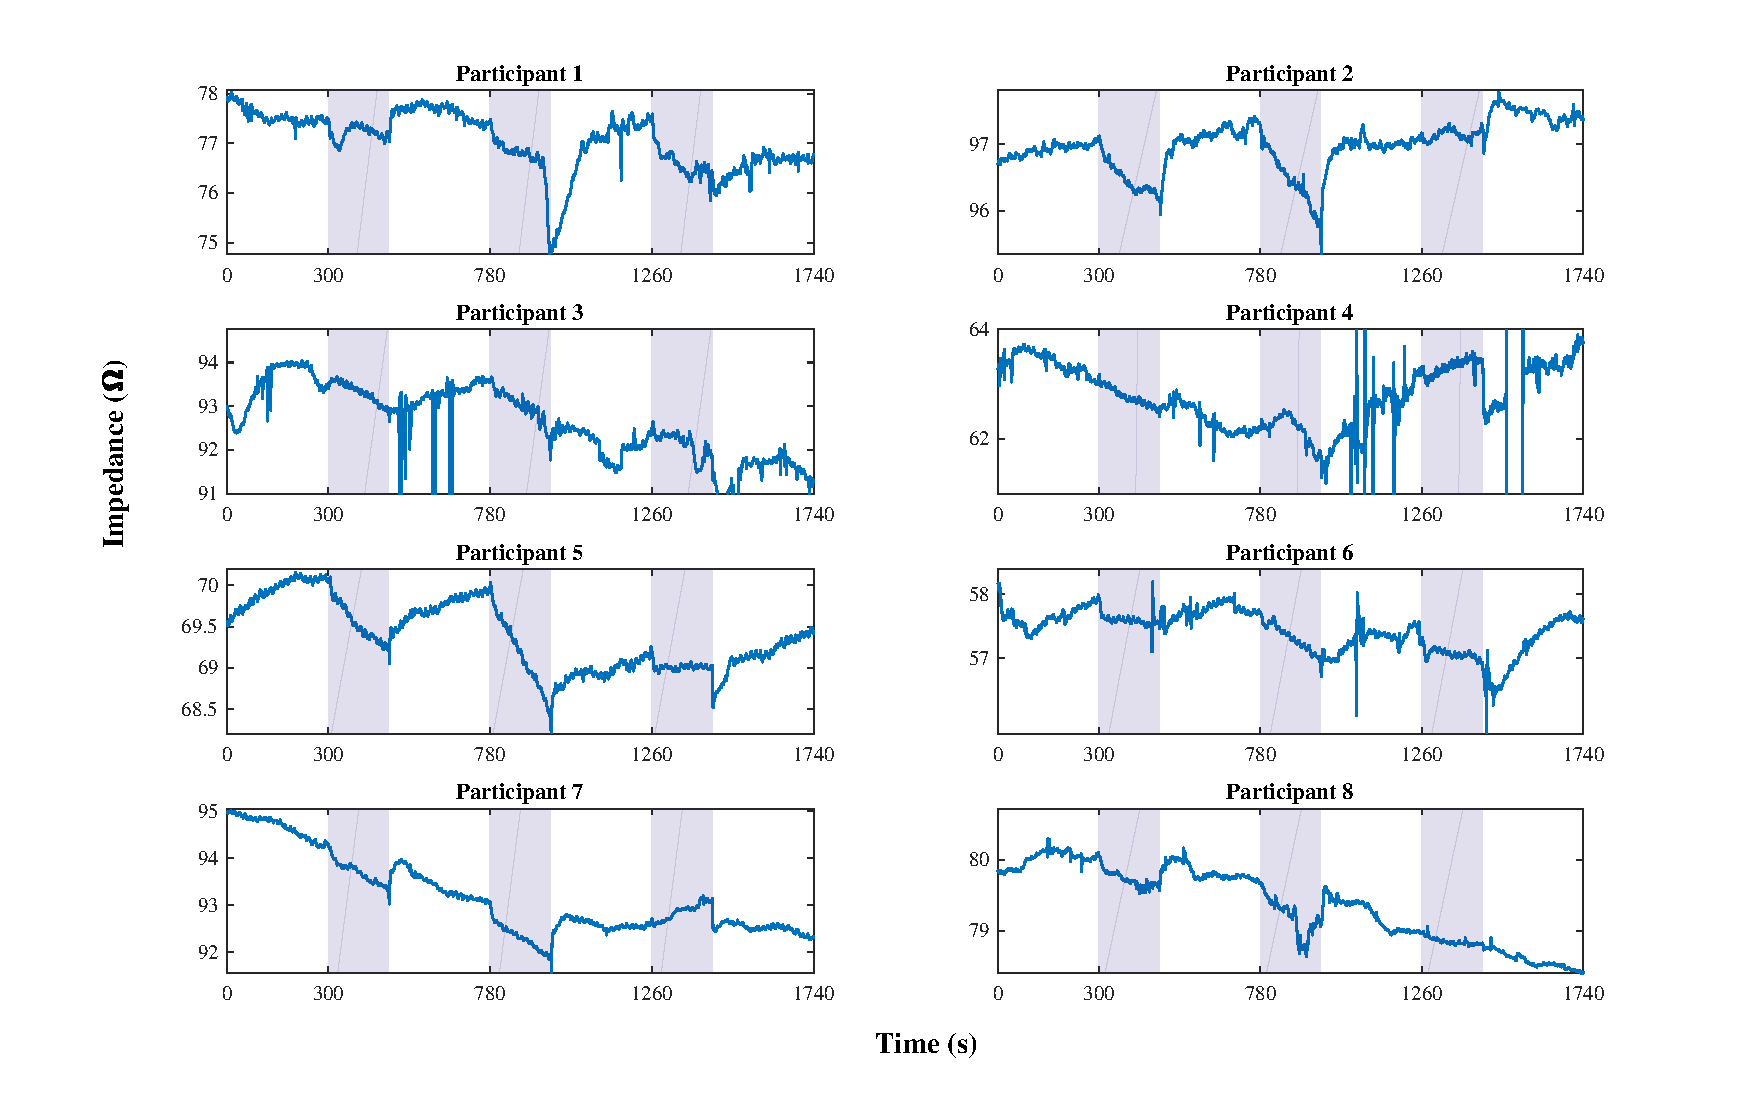
\includegraphics[width=\textwidth,height=\textheight,keepaspectratio]{figure1}    
	\caption[Measurements of the basal impedance during the whole study]{Basal impedance of all the participants during the whole study. The data collected has been divided into regions. The regions (1,3,5 and 7) in white colour represent baseline measurements. The shaded areas (regions 2,4 and 6) represent occlusive events.  }
	\label{fig:rb:all_participants} 
\end{figure}

\begin{sidewaystable}[!htbp] %tbl:Z_regions
	\caption[Mean basal impedance is divided in seven regions]{Mean basal impedance is divided into seven regions according to the time of the event. Measurements include standard deviation from each value. }
	\label{tbl:Z_regions}
	\centering
	\begin{tabular}    {l
			*{7}{S[table-format=2.2]@{\,\( \pm \)\,}S[table-format=1.2]} %Format for Z+-std
		}
		\toprule
		&\multicolumn{2}{c}{\textbf{Region 1}}&\multicolumn{2}{c}{\textbf{Region 2}}&\multicolumn{2}{c}{\textbf{Region 3}}&\multicolumn{2}{c}{\textbf{Region 4}}&\multicolumn{2}{c}{\textbf{Region 5}}&\multicolumn{2}{c}{\textbf{Region 6}}&\multicolumn{2}{c}{\textbf{Region 7}}\\
		&\multicolumn{2}{c}{\small{\SIrange{0}{300}{\second}}}&\multicolumn{2}{c}{\small{\SIrange{300}{480}{\second}}}&\multicolumn{2}{c}{\small{\SIrange{480}{780}{\second}}}&\multicolumn{2}{c}{\small{\SIrange{780}{960}{\second}}}&\multicolumn{2}{c}{\small{\SIrange{960}{1260}{\second}}}&\multicolumn{2}{c}{\small{\SIrange{1260}{1440}{\second}}}&\multicolumn{2}{c}{\small{\SIrange{1440}{1740}{\second}}} \\                                   &\multicolumn{2}{c}{$\bar{\textrm{Z}}$ [\si{\ohm}]}&\multicolumn{2}{c}{$\bar{\textrm{Z}}$ [\si{\ohm}]}&\multicolumn{2}{c}{$\bar{\textrm{Z}}$ [\si{\ohm}]}&\multicolumn{2}{c}{$\bar{\textrm{Z}}$ [\si{\ohm}]}&\multicolumn{2}{c}{$\bar{\textrm{Z}}$ [\si{\ohm}]}&\multicolumn{2}{c}{$\bar{\textrm{Z}}$ [\si{\ohm}]}&\multicolumn{2}{c}{$\bar{\textrm{Z}}$ [\si{\ohm}]}\\\midrule
		Participant 1  &  77.59  &    0.17  &  77.24   &   0.14  &  77.67  &    0.16   & 76.73  &    0.48  &  76.84   &   0.79  &  76.64  &    0.28  &  76.61   &   0.22\\
		Participant 2  &  96.97  &    0.09  &  96.54   &   0.22  &  97.15  &    0.23   & 96.52  &    0.37  &  97.01   &   0.18  &  97.15  &    0.07  &  97.50   &   0.13\\
		Participant 3  &  93.54  &    0.50  &  93.37   &   0.23  &  93.08  &    0.94   & 93.04  &    0.34  &  92.21   &   0.30  &  92.14  &    0.30  &  91.43   &   0.85\\
		Participant 4  &  63.44  &    0.19  &  62.80   &   0.16  &  62.40  &    0.24   & 62.21  &    0.25  &  62.47   &   0.54  &  63.37  &    0.13  &  66.03   &   6.47\\
		Participant 5  &  69.97  &    0.17  &  69.60   &   0.23  &  69.77  &    0.16   & 69.23  &    0.41  &  68.99   &   0.13  &  69.02  &    0.04  &  69.21   &   0.21\\
		Participant 6  &  57.68  &    0.17  &  57.63   &   0.08  &  57.77  &    0.11   & 57.35  &    0.20  &  57.31   &   0.19  &  57.08  &    0.07  &  57.22   &   0.41\\
		Participant 7  &  94.72  &    0.24  &  93.75   &   0.23  &  93.46  &    0.28   & 92.37  &    0.26  &  92.63   &   0.11  &  92.87  &    0.17  &  92.57   &   0.10\\
		Participant 8  &  80.04  &    0.11  &  79.75   &   0.10  &  79.85  &    0.11   & 79.23  &    0.25  &  79.24   &   0.21  &  78.87  &    0.05  &  78.60   &   0.11\\\bottomrule
	\end{tabular}
\end{sidewaystable}

%%********************************** % Section 5.2.1 ******************************************
\subsection{Baseline impedance}
\label{section results 2.1}
The iPG device recorded the impedance during the first five minutes of data logging. The device was able to detect the forearm's segment impedance quite remarkably. The values obtained fell within the resistive value estimated by the literature \mynote{Find some papers with results about the impedance of the forearms}. The table \ref{tbl:basal_impedace:region1} describes the basal impedance during the first five minutes of data. 

\begin{table}[!htbp]
	\caption{Basal impedance during the first five minutes of data with statistical values.}
	\label{tbl:basal_impedace:region1}
	
	\centering
	\begin{tabular}        
		{
			l
			c
			S[table-format=2.2]@{\,\( \pm \)\,}S[table-format=1.2] %Format for Z+-std
			*{2}{S[table-format=2.2]} 
		}
		\toprule
		& \textbf{Size} & \multicolumn{2}{c}{\textbf{ $\bar{\textrm{Z}}$ [\si{\ohm}]}} & \textbf{Max [\si{\ohm}]} & \textbf{Min [\si{\ohm}]} \\ \midrule
		Participant 1  &  278  &  77.59  &  0.17  &  78.04  &  77.37\\
		Participant 2  &  295  &  96.97  &  0.09  &  97.17  &  96.76\\
		Participant 3  &  275  &  93.54  &  0.50  &  94.06  &  92.44\\
		Participant 4  &  329  &  63.44  &  0.19  &  63.77  &  63.02\\
		Participant 5  &  288  &  69.97  &  0.17  &  70.20  &  69.56\\
		Participant 6  &  331  &  57.68  &  0.17  &  58.21  &  57.33\\
		Participant 7  &  340  &  94.72  &  0.24  &  95.05  &  94.27\\
		Participant 8  &  353  &  80.04  &  0.11  &  80.30  &  79.82\\ \bottomrule
	\end{tabular} 
\end{table} 

There are different aspects of the geometry that could affect the impedance reading. There have been several studies which demonstrated how the distance between electrodes affects readings\mynote{Add reference to studies impedance vs. length}. This study portrayed that impedance was influenced by the forearm's circumference, as well as the distance between the potential electrodes. Figure \ref{fig:C_vs_Z} indicates that there is an inverse relation between circumference and impedance. The smaller the forearm's circumference, the higher the resistivity. On the other hand, there is a direct relation between the distance between the potential electrodes and the resistivity of the segment as depicted in \ref{fig:l_vs_Z}.

In contrast, when comparing total volume measured and mean resistivity of the segment, there is a slight drop of impedance, but it is not a clear \nknote{tendency dropped in this sentence doesnt make sense}tendency (see figure \ref{fig:Ve_vs_Z}). The data points are scattered depicting no clear trend. This lack of bias can be explained as the fat content can affect impedance measurements. As explained by xxx \mynote{Add reference about the affinity of fat and impedance}, fat is a good conductor of electricity. Hence, fat content does not allow to show a clear tendency in impedance and volume\nknote{review this sentence}. Nevertheless, in the end, the change of volume from the first basal impedance is going to be caused by the blood streaming trough the vessels.  

\begin{figure*}[!htbp]
	\centering
	\begin{subfigure}[t]{0.48\textwidth}
		\centering
		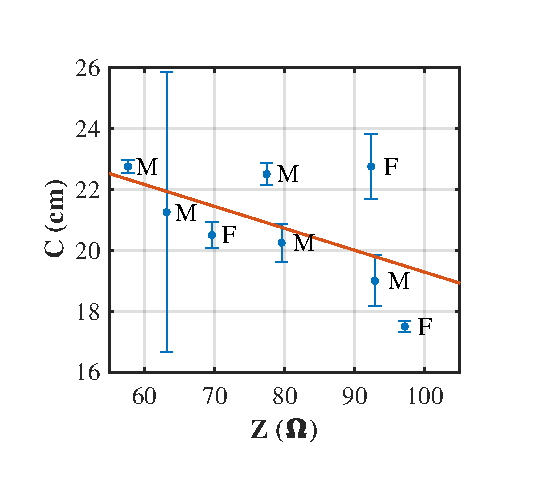
\includegraphics[height=5cm]{figure2a}
		\caption{Relationship between forearm circumference and mean basal impedance}
		\label{fig:C_vs_Z}
	\end{subfigure}%
	~ 
	\begin{subfigure}[t]{0.48\textwidth}
		\centering
		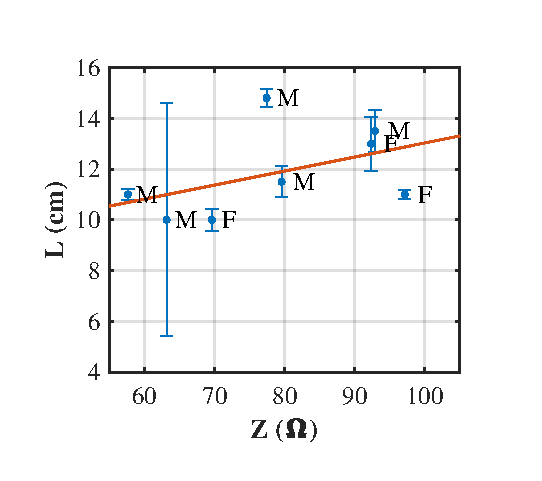
\includegraphics[height=5cm]{figure2b}
		\caption{Relationship between distance sensing electrodes and mean basal impedance}
		\label{fig:l_vs_Z}
	\end{subfigure}
	~ 
	\begin{subfigure}[t]{0.48\textwidth}
		\centering
		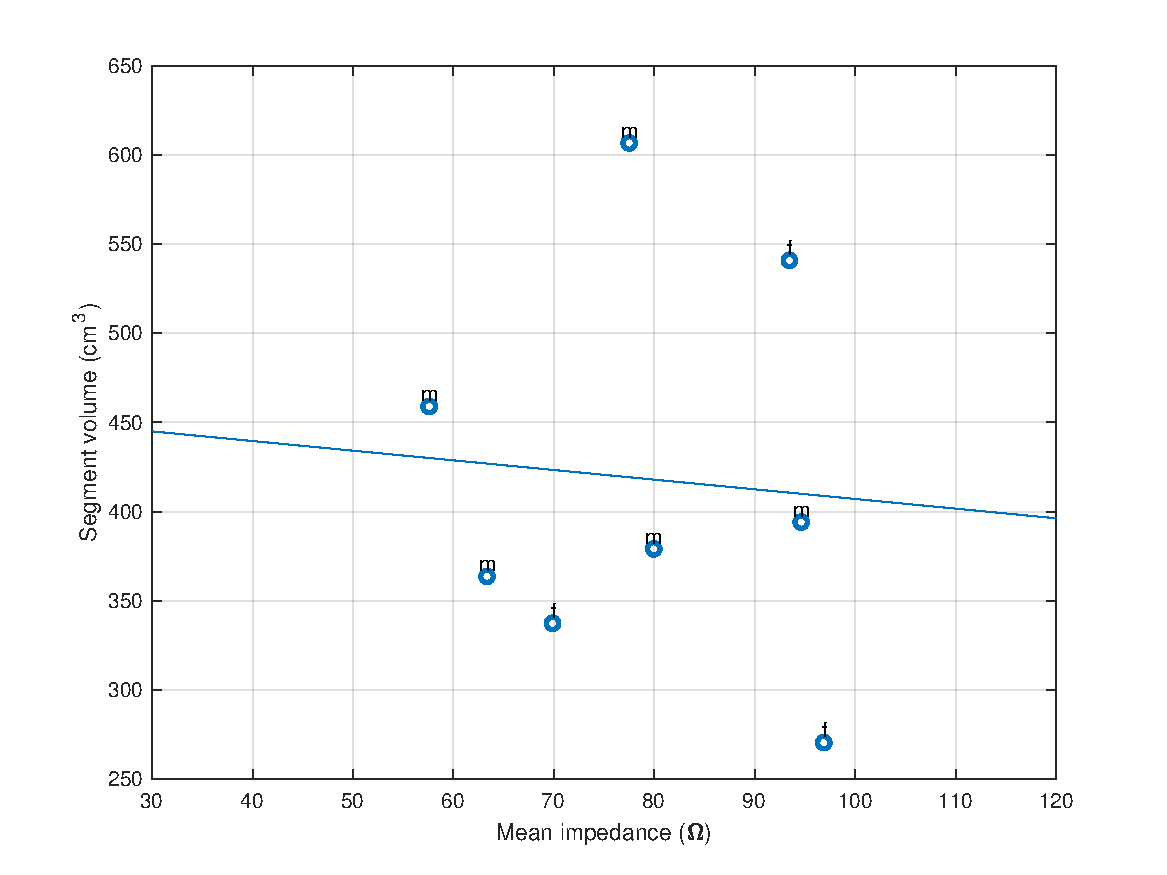
\includegraphics[height=5cm]{figure2c}
		\caption{Relation between forearms segment volume and mean basal resistivity}
		\label{fig:Ve_vs_Z}
	\end{subfigure}
	\caption{Relation between circumference, length and total segment's volume and mean basal impedance}
	\label{fig:relation_geometry_vs_impedance}
\end{figure*}


%%********************************** % Section 5.2.2 ******************************************
\subsection{Mean impedance measurement during venous occlusion}
\label{section results 2.2}
During the following three minutes after the impedance, venous occlusion occurred.\nknote{I think you made an error in explaining what you are trying to say here} As can be seen in figure \ref{fig:rb:all_participants}, all the participants experienced a decrease in basal impedance during this time. Most of the subjects presented a linear impedance decrease trend during the occlusion. However, some of the measurements were clearly affected by motion artefact. Participants one and six are an example of this. 

In participant one, resistance fell immediately as the occlusion occurred. Nevertheless, after a minute the subject moved his arm correcting the trend. Then, impedance continued the trend again. Furthermore,  participant six also showed a similar response when the arm moved. 

Figure \ref{fig:normalise:venous_occlusion} describes how the impedance behaved during the occlusion for all participants. The graph has been normalised to compare the resistivity reduction.  A linear regression was performed in the data to demonstrate the ratio of change during the occlusion.

\begin{figure}[!htbp]
	\centering
	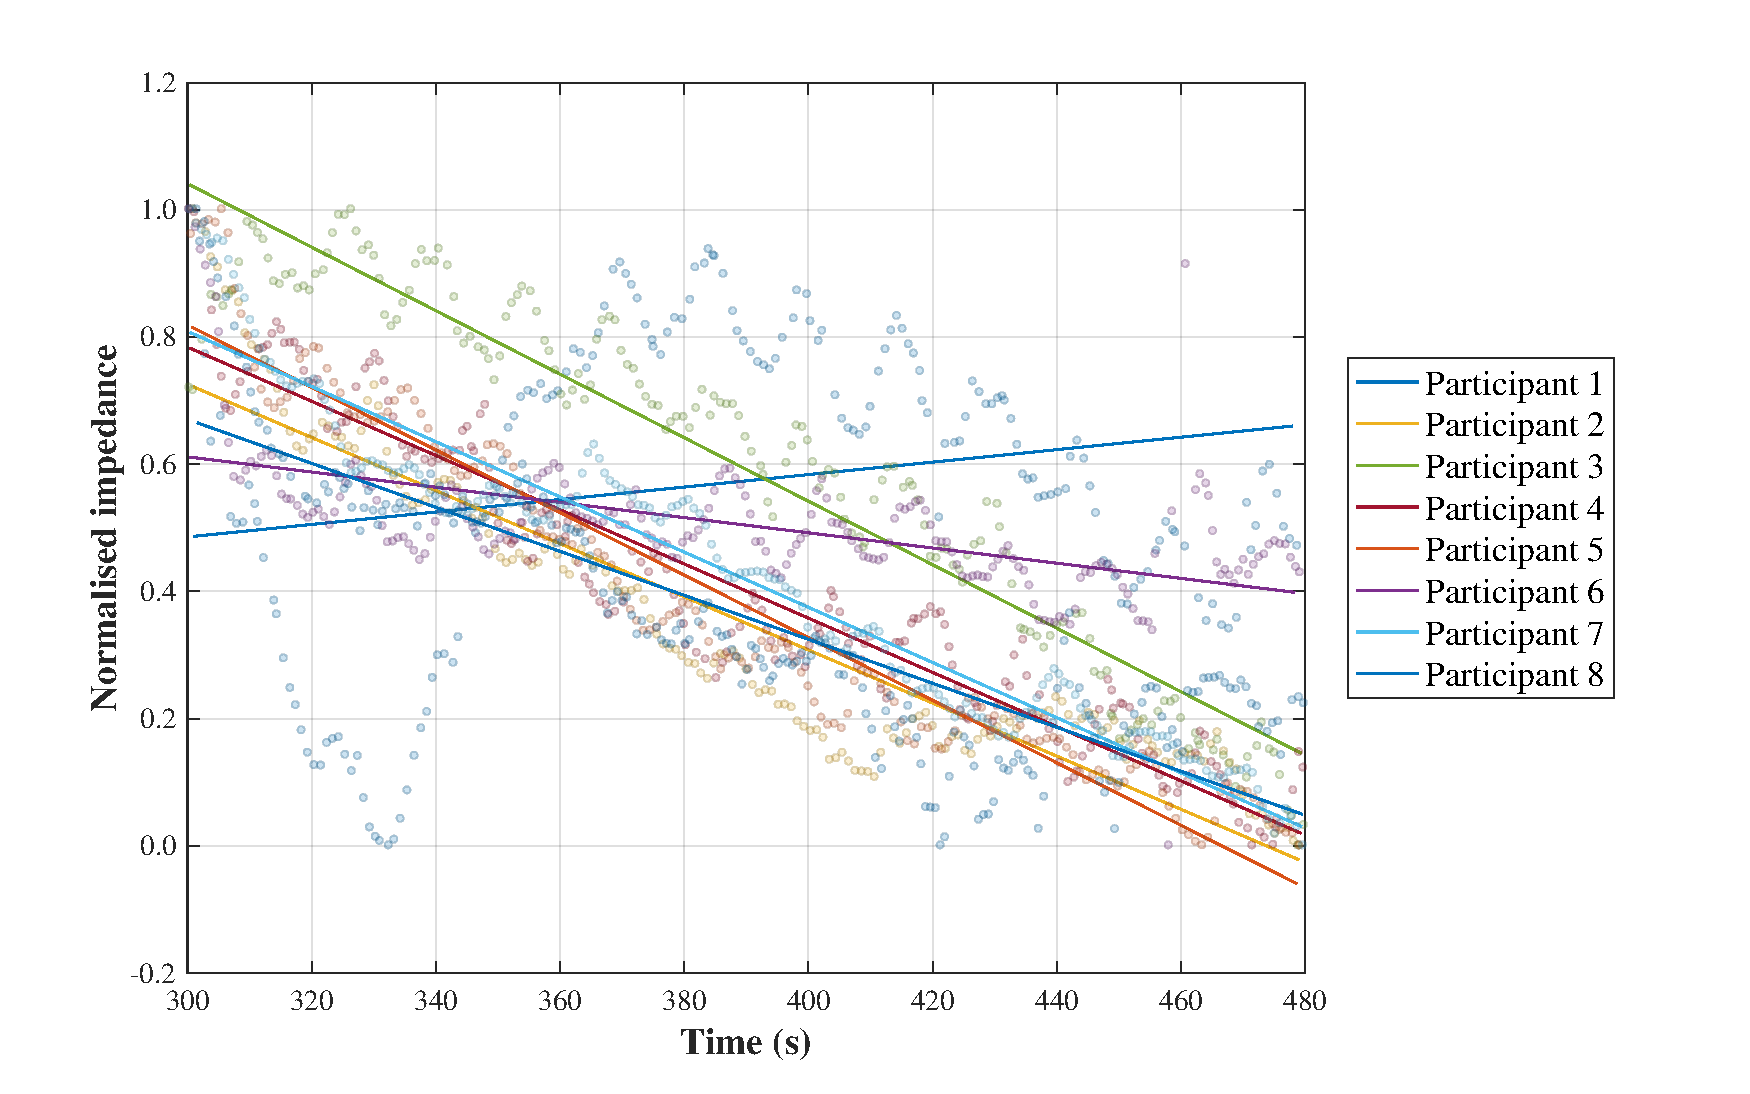
\includegraphics[width=\textwidth,keepaspectratio]{figure3}    
	\caption{Normalise plot of impedance decrease during venous occlusion.}
	\label{fig:normalise:venous_occlusion}
\end{figure}  

The table \ref{tbl:venous_occlusion:region2} overviews the results obtained from the linear regression. The value $Z_1$ illustrates the value of the impedance as the blockage started and $Z_{end}$ the resistance value at the end of the test.  $\Delta Z$ (mean \SI{-0.632(0068)}{\ohm}) is the variation of impedance during the \SI{3}{\minute} that the experiment lasted. The slope demonstrates how much resistance is changing during each beat  (mean $-0.00271\pm3.415e^{-6}\Omega\textrm{/s}$). 

\begin{table}[!htbp]
	\caption{Linear regression result for all participants during venous occlusion.}
	\label{tbl:venous_occlusion:region2}
	\centering
	\begin{tabu}{lcccccc}
		\toprule
		& \textbf{Slope [\si{\ohm/\second}]} & \textbf{Intercept [\si{\ohm}]} & \textbf{$R^2$} & \textbf{$Z_1$ [\si{\ohm}]} & \textbf{$Z_{end}$ [\si{\ohm}]} & \textbf{ $\Delta Z$ [\si{\ohm}]} \\ \midrule
		Participant 1  &   0.00057  &  77.02   &     0.037  &  77.49  &  77.18  &  -0.31\\
		Participant 2  &  -0.00395  &  98.09   &     0.867  &  97.16  &  96.21  &  -0.95\\
		Participant 3  &  -0.00421  &  95.01   &     0.917  &  93.47  &  92.89  &  -0.58\\
		Participant 4  &  -0.00296  &  63.96   &     0.920  &  63.22  &  62.61  &  -0.61\\
		Participant 5  &  -0.00427  &  71.26   &     0.936  &  70.10  &  69.27  &  -0.83\\
		Participant 6  &  -0.00085  &  57.96   &     0.322  &  57.98  &  57.57  &  -0.40\\
		Participant 7  &  -0.00427  &  95.42   &     0.934  &  94.33  &  93.34  &  -0.98\\
		Participant 8  &  -0.00173  &  80.43   &     0.752  &  80.07  &  79.68  &  -0.39\\ \bottomrule
	\end{tabu} 
\end{table}

From the statistical analysis displayed one can conclude the following: as explained previously, the slopes from participants 1 and 6 were affected by the motion artefact. Nevertheless, these trends seemed corrected after one minute of recordings (\SI{360}{\second}). Their slopes were quite far away from the mean value (\num{-0.00271}$\pm$\SI{3.415e-06}{\ohm\per\second}). On the other hand, the rest of the signals showed a similar trend. \mynote{Review this paragraph. It seems to be very similar to the previous one.}


%%********************************** % Section 5.2.3 ******************************************
\subsection{Mean impedance data during partial arterial occlusion}
\label{section results 2.3}
During partial arterial occlusion (\SIrange{480}{760}{\second}), the incoming arterial flow is restricted causing a slow filling of the forearm. This mechanical blocking induces an uncomfortable feeling to the participants, some of them felt numbness in the arm.  As can be seen from figure \ref{fig:rb:all_participants}, in most of the participants there is an apparent drop in impedance during the action \nknote{what action?}. Although participant one moved his muscles, creating a sharp fall before releasing the pressure, partaker four also showed a slight increment of impedance in the middle of this part of the test. 

Figure \ref{fig:normalise:arterial_occlusion} shows the normalised resistivity decrease for all the participants. Table \ref{tbl:arterial_occlusion:region4} shows the values of the linear regression for the data.   All in all, it is clear that the decrease of resistivity is sharper in this part of the experiment compared to venous occlusion.  In fact, when this data is compared to venous information, the average slope is nearly twice as big (mean \num{-0.00536}$\pm$\SI{2.853e-06}{\ohm\per\second}). Also, the total change of impedance ($\Delta Z$) was almost doubled in all participants, except participant four, in which the value decreased.  

\begin{table}[!htbp]
	\caption{Linear regression result for all participants during partial arterial occlusion.}
	\label{tbl:arterial_occlusion:region4}
	\centering
	\begin{tabu}{lcccccc}
		\toprule
		& \textbf{Slope [\si{\ohm/\second}]} & \textbf{Intercept [\si{\ohm}]} & \textbf{$R^2$} & \textbf{$Z_1$ [\si{\ohm}]} & \textbf{$Z_{end}$ [\si{\ohm}]} & \textbf{ $\Delta Z$ [\si{\ohm}]} \\ \midrule
		Participant 1  &  -0.00656  &   82.44    &   0.519  &  77.51  &  74.91  &  -2.60 \\
		Participant 2  &  -0.00706  &  102.67    &   0.965  &  97.29  &  95.75  &  -1.54 \\
		Participant 3  &  -0.00601  &   98.28    &   0.858  &  93.61  &  92.20  &  -1.41 \\
		Participant 4  &  -0.00327  &   65.05    &   0.474  &  62.25  &  61.81  &  -0.44\\
		Participant 5  &  -0.00767  &   75.89    &   0.989  &  70.05  &  68.50  &  -1.55\\
		Participant 6  &  -0.00366  &   60.53    &   0.939  &  57.74  &  56.88  &  -0.85\\
		Participant 7  &  -0.00490  &   96.64    &   0.969  &  93.11  &  92.02  &  -1.09\\
		Participant 8  &  -0.00381  &   82.54    &   0.627  &  79.70  &  79.10  &  -0.59\\ \bottomrule
	\end{tabu} 
\end{table}

The linear regression of this region of the signal showed an apparent straight tendency for most of the participants. Most of the signals can be represented as a negative tilt line ($R^2 \geq 0.858 $), except members one, four and eight ($R^2 \leq 0.627 $).

\mynote{Check about what happens during partial arterial occlusion. Slow filling of the forearm. This information should also be added to the Medical Background}

\begin{figure}[!htbp]
	\centering
	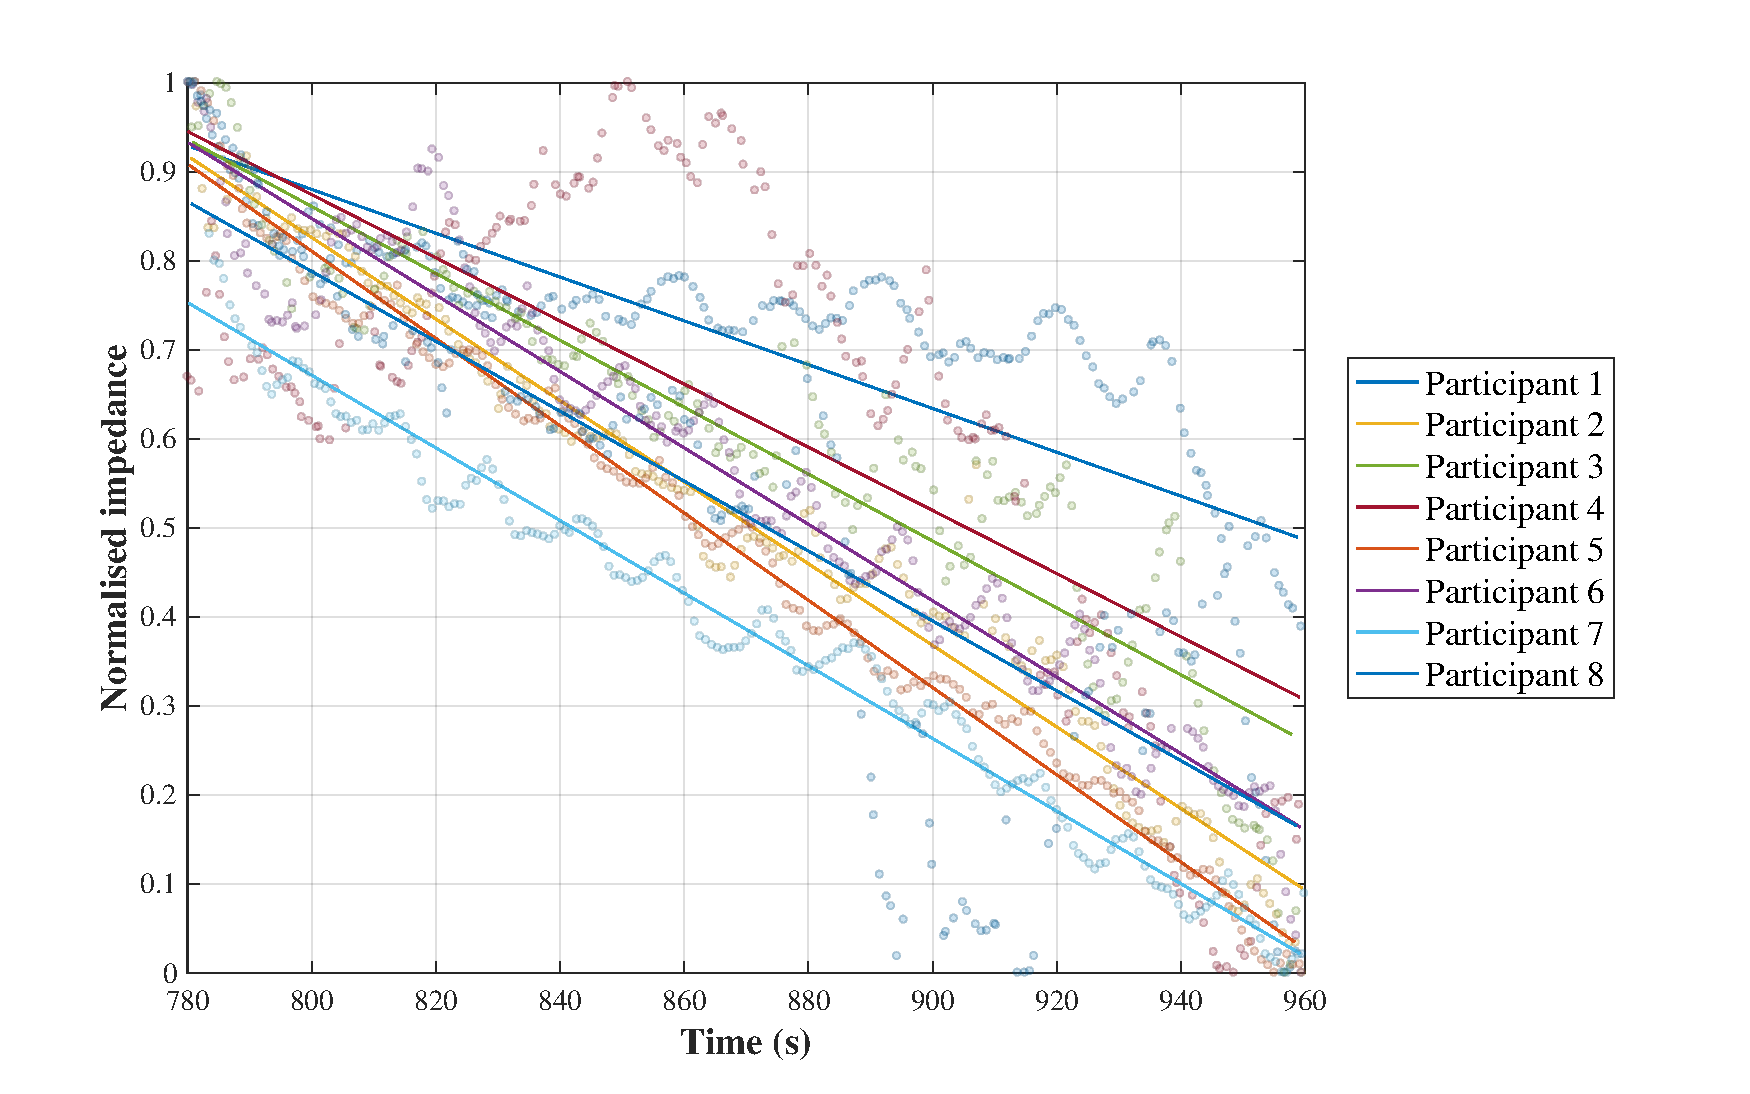
\includegraphics[width=0.9\textwidth,height=0.9\textheight,keepaspectratio]{figure4}    
	\caption{Normalise plot of impedance decrease during partial arterial occlusion.}
	\label{fig:normalise:arterial_occlusion}
\end{figure}
\mynote{Figure \ref{fig:normalise:venous_occlusion} is temporary. It needs to be improved by naming axis}



%%********************************** % Section 5.2.4 ******************************************
\subsection{Mean impedance data during total occlusion}
\label{section results 2.4}
Producing a total occlusion (between \SIrange{1260}{1440}{\second}) in the upper arm stops the blood inflow completely under the obstructed section. This test caused much discomfort to most of the participants, which made them move their limbs voluntary. Because there is no blood pooling during this part of the experiment it is expected to not see a common tendency in impedance variation. Additionally, the mean restive value is equivalent to the impedance of the tissue components within the segment plus the impedance of the residual blood in the forearm. However, when a change of resistivity happens this is mostly caused by the participant's re-accommodation rather than a physiological variable. 

After analysing the data obtained (see  Table \ref{tbl:total_occlusion:region6} and figure \ref{fig:normalise:total_occlusion}), it can be noticed that there is not a defined trend for most of the signals. The slopes and deltas computed show a variation between negative and positive values. Therefore, it can be concluded that there is not an indication of a clear bias common to the signals. 

\begin{table}[!htbp]
	\caption{Linear regression result for all participants during total occlusion.}
	\label{tbl:total_occlusion:region6}
	\centering
	\begin{tabu}{lcccccc}
		\toprule
		& \textbf{Slope [\si{\ohm/\second}]} & \textbf{Intercept [\si{\ohm}]} & \textbf{$R^2$} & \textbf{$Z_1$ [\si{\ohm}]} & \textbf{$Z_{end}$ [\si{\ohm}]} & \textbf{ $\Delta Z$ [\si{\ohm}]} \\ \midrule
		Participant 1  &  -0.00431  &  82.44   &      0.652 &   77.58 &  76.33  &   -1.25\\ 
		Participant 2  &   0.00044  &  96.55   &      0.105 &   97.22 &   97.28 &    0.07\\
		Participant 3  &  -0.00432  &  97.99   &      0.587 &   92.57 &   91.45 &   -1.12\\
		Participant 4  &   0.00226  &  60.31   &      0.789 &   63.31 &   63.45 &    0.14\\
		Participant 5  &  -0.00002  &  69.04   &     -0.005 &   69.22 &   69.01 &   -0.21\\
		Participant 6  &  -0.00096  &  58.38   &      0.457 &   57.34 &   56.95 &   -0.40\\
		Participant 7  &   0.00310  &  88.70   &      0.899 &   92.78 &   93.11 &    0.33\\
		Participant 8  &  -0.00080  &  79.94   &      0.644 &   78.97 &   78.82 &   -0.15\\ \bottomrule
	\end{tabu} 
\end{table}

The impedance plethysmography signal can confirm the absence of blood flow. On section xxx \mynote{Add reference in plethysmography that shows the waveforms} is shown the lack of peaks in the signal. 

\mynote{Check about what happens during partial arterial occlusion. Slow filling of the forearm. This information should also be added to the Medical Background}

\begin{figure}[!htbp]
	\centering
	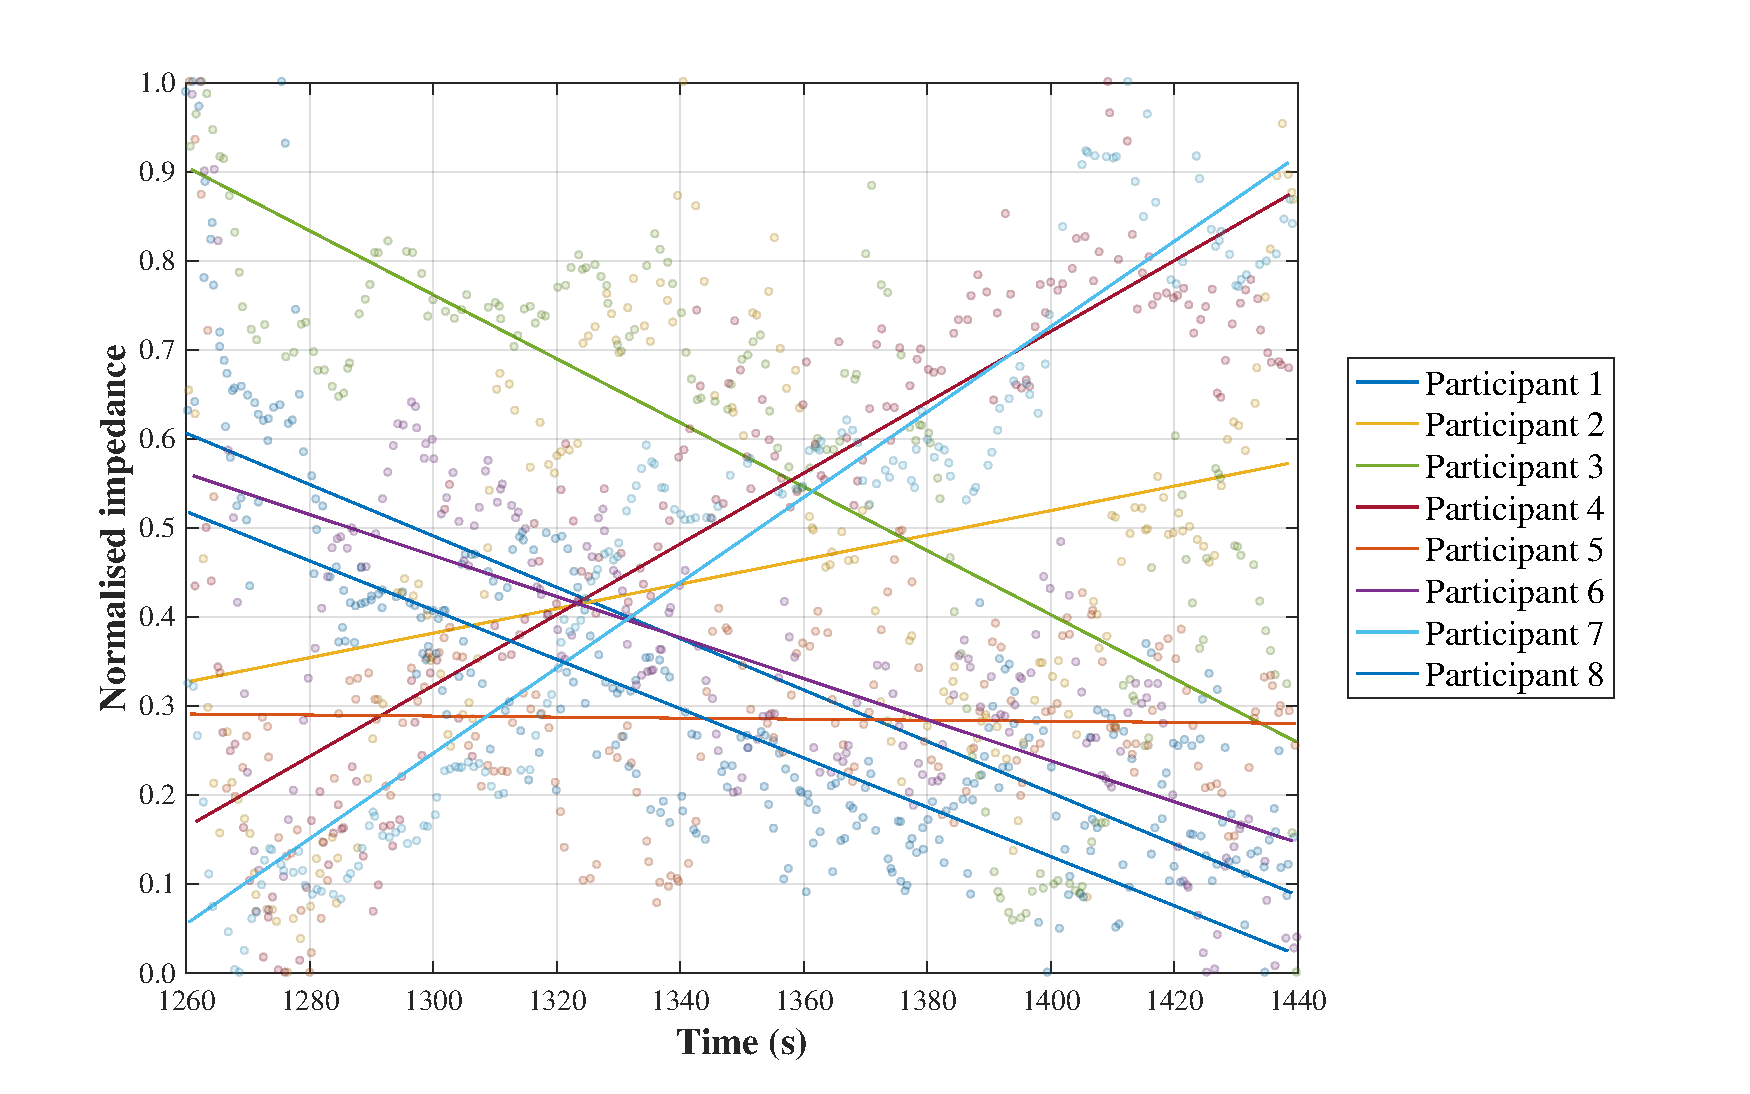
\includegraphics[width=0.9\textwidth,height=0.9\textheight,keepaspectratio]{figure5}    
	\caption{Normalise plot of impedance decrease during total occlusion.}
	\label{fig:normalise:total_occlusion}
\end{figure}
\mynote{Figure \ref{fig:normalise:venous_occlusion} is temporary. It needs to be improved by naming axis}


%%********************************** % Section 5.3 ******************************************
%\pagebreak
\section{Plethysmography impedance results}
\label{section results 3}
The iPG device provided a port illustrated as $Z_{AC}$ \mynote{To double check if this is the correct port name from the initial description} which provided a high-resolution view of the plethysmography waveform.  In fact, as shown in the design section xxx \mynote{Reference a section to this part}, the signal was amplified nearly 2500 times. Hence, the waveform obtained provides more detail and also improves rejection \nknote{?rejection correct word?} to noise.

The waveforms obtained through this method reproduce the change of volume per heart beat within the sensing electrodes. The filling of the blood vessels creates small changes in resistivity that change with the circulatory cycle (see section xxx \mynote{I have to add a section to describe how plethysmography is related to blood cycle}). The waveforms presented in this part were analysed using the decomposing method described in section \ref{section procedure 3.2}. \mynote{I need to add more detail within that section}. Five different points on the waveform were identified by the algorithm.

The waveform produced by the device is inverted as represented by various other plethysmography devices such as photoplethysmography. During the systolic cycle, the blood vessels expand allowing more blood volume. Hence, the impedance drops proportionally to the amount of blood because the forearm's segment is more electrically conductive. On the other hand, during the diastolic cycle, blood vessels empty causing a reduction the quantity of blood contained in the segment. As a result, the impedance increases.  

Treating the digital signal required to remove noisy components of the waveform. As described in section xxx\mynote{Add section were the digital processing was performed}, the signal was levelled to zero.  From there, the points of interest were calculated to identify the different changes in the waveform. The analysis of the plethysmographic wave was performed by averaging all the waveforms detected by the algorithm. The following discussion represents the change of form from a non-occlusion state to an occluded one. At the end of the section, the results of all participants will be summarised \mynote{I could add a description of how the signal looks. For instance by adding 10 or 20 beats to show how the device worked.}.

%%********************************** % Section 5.3.1 ******************************************
\subsection{Plethysmography waveform change from baseline to venous occlusion}
\label{section results 3.1}
This analysis corresponds to the waveform during baseline (\SIrange{0}{300}{\second}), venous occlusion (\SIrange{300}{480}{\second}) and return to control signal (\SIrange{480}{780}{\second}). This graph was obtained by averaging all the plethysmography waveforms detected by the algorithm and described in detail in section xxx \mynote{Add reference where the waveform detection algorithm is explained}. In the end, all the peaks were averaged obtaining the mean waveform displayed in the figure for baseline and venous occlusion.

Figure \ref{fig:iPG_venous_baseline} shows the common impedance plethysmography waveform, with indicators of their amplitudes at different points of interest. The distance between systolic peak (Point A) to dicrotic notch (Point B) and diastolic peak (Point C) was calculated. This value was later transposed into the occlusion wave to identify their values during the venous occlusion test.

As detailed in section xxx \mynote{Add note describing how the waveform is composed}, a plethysmography waveform consists of three distinct parts. The systolic peak, dicrotic notch and the diastolic peak, have been identified in figure \ref{fig:iPG_venous_baseline}. From a qualitative point of view, one can notice that there is a difference in the morphology of the waveform. An analysis on the change of each these points are presented in figure \ref{fig:iPG_change_points_venous} and analysed in detail as follows.

\begin{figure*}[!htbp]
	\centering
	\begin{subfigure}[t]{0.48\textwidth}
		\centering
		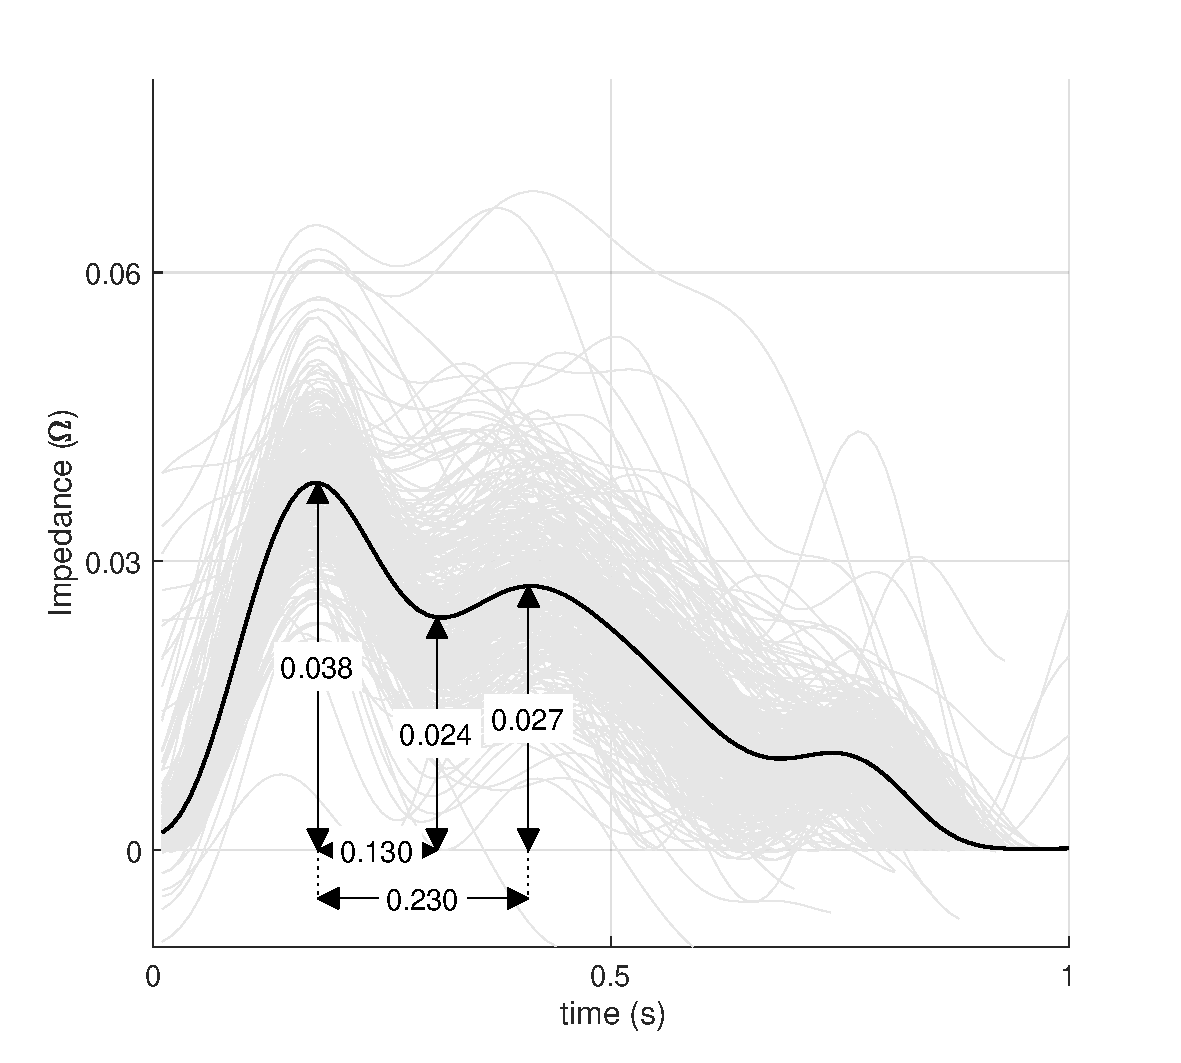
\includegraphics[height=6cm]{figure6a}
		\caption{Average plethysmography waveform for baseline region 1 (\SIrange{0}{300}{\second})}
		\label{fig:iPG_venous_baseline}
	\end{subfigure}%
	~ 
	\begin{subfigure}[t]{0.48\textwidth}
		\centering
		\includegraphics[height=6cm]{figure6b}
		\caption{Average plethysmography waveform during venous occlusion region 2 (\SIrange{300}{480}{\second})}
		\label{fig:iPG_venous_occlusion}
	\end{subfigure}
	\caption{Plethysmography waveform of the participant seven between baseline and venous occlusion}
	\label{fig:iPG_venous}
\end{figure*}

\begin{figure*}[!htpb]
	\centering
	\begin{subfigure}[t]{0.48\textwidth}
	\centering
		\includegraphics[height=6cm,keepaspectratio]{figure7a2}    
		\caption{Change of amplitude of the waveform at point A.}
		\label{fig:change_A_venous}
	\end{subfigure}%
	~ 
	\begin{subfigure}[t]{0.48\textwidth}
		\centering
		\includegraphics[height=6cm,keepaspectratio,keepaspectratio]{figure7b2}    
		\caption{Change of amplitude of the waveform at point B}
		\label{fig:change_B_venous}
	\end{subfigure}
	~
	\begin{subfigure}[t]{0.48\textwidth}
		\centering
		\includegraphics[height=6cm,keepaspectratio]{figure7c2}    
		\caption{Change of amplitude of the waveform at point C}
		\label{fig:change_C_venous}
\end{subfigure}%
	\caption{Changes of the impedance peak values during baseline, partial arterial occlusion and return to baseline for points A,B and C.}
	\label{fig:iPG_change_points_venous}
\end{figure*}

\subsubsection{Changes in systolic peak (Point A)}
\label{section results 3.1.1}
Most of the signals showed a change in the height of their top systolic values after inflating the cuff to the values shown in column \textit{Occlusion 1} in Table~\ref{tbl:occlusions}. After quantifying the amplitude of the signal at this point, an increase in their peak value can be seen. Indeed \SI{87}{\percent} of the participants showed an increment in resistance with an average of \SI{20.93}{\percent}, only participant 8 was an exception where impedance decreased \SI{-11.11}{\percent}. Then, when the cuff's pressure was released, all the participants showed a decline of the peak value with an average of \SI{-27.88}{\percent}, returning to similar values prior to the occlusion. Figure \ref{fig:change_A_venous} indicates the relation of change in amplitude during the three conditions. 

\mynote{If using box then I have to double check the data obtained. Boxplot uses median not mean}

\begin{table}[!htbp]
	\caption{Change of amplitude of the waveform at peak A during the transition from baseline to venous occlusion.}
	\label{tbl:change_A_venous}
	\centering\small
\begin{tabular}{l
				*{3}{S[table-format=1.4]@{\,\( \pm \)\,}S[table-format=1.4]} %Format for Z+-std
		       cc}
	\toprule
	& \multicolumn{2}{c}{\multirow{2}{*}{\textbf{Baseline [\si{\ohm}]}}}
	& \multicolumn{2}{c}{\multirow{2}{*}{\textbf{Occlusion [\si{\ohm}]}}}
	& \multicolumn{2}{c}{\multirow{2}{*}{\textbf{Baseline [\si{\ohm}]}}}
	& \multicolumn{2}{c}{\textbf{Change}} \\
	& \multicolumn{2}{c}{}
	& \multicolumn{2}{c}{}
	& \multicolumn{2}{c}{}
	&\textbf{R1-R2}&\textbf{R2-R3}\\\midrule
	Participant 1    &     0.0283    &     0.0233    &     0.0342    &     0.0191    &     0.0305    &     0.0305    &      20.93\%    &     -13.29\%    \\
	Participant 2    &     0.0491    &     0.0102    &     0.0595    &     0.0140    &     0.0449    &     0.0449    &      21.01\%    &     -29.68\%    \\
	Participant 3    &     0.0346    &     0.0351    &     0.0374    &     0.0144    &     0.0294    &     0.0294    &       7.91\%    &     -22.89\%    \\
	Participant 4    &     0.0252    &     0.0303    &     0.0272    &     0.0139    &     0.0222    &     0.0222    &       7.98\%    &     -19.87\%    \\
	Participant 5    &     0.0345    &     0.0112    &     0.0481    &     0.0098    &     0.0376    &     0.0376    &      39.68\%    &     -30.69\%    \\
	Participant 6    &     0.0233    &     0.0105    &     0.0306    &     0.0124    &     0.0251    &     0.0251    &      31.33\%    &     -23.52\%    \\
	Participant 7    &     0.0359    &     0.0080    &     0.0537    &     0.0081    &     0.0365    &     0.0365    &      49.72\%    &     -47.78\%    \\
	Participant 8    &     0.0237    &     0.0094    &     0.0211    &     0.0091    &     0.0127    &     0.0127    &     -11.11\%    &     -35.30\%    \\  \bottomrule
\end{tabular} 
\end{table}


\subsubsection{Changes in dicrotic notch peak (Point B)}
\label{section results 3.1.2}
The dicrotic notch point is located between the systolic and diastolic peaks. The forearm's iPG waveform looks like a dip as illustrated in figure \ref{fig:iPG_venous}. This locality in the waveform has been identified in this document as point B. 

The value of this signal changed from baseline when venous occlusion occurred. After that, when cuff was deflated, all impedance peaks decreased. According to the data shown on Table \ref{tbl:change_B_venous}, one can see that most of the signals (\SI{75}{\percent}) show an increase in their value. Certainly, there was an increment in impedance with an average of \SI{29.30}{\percent}. However, partakers two and four noted a slight decrease in their values \SI{-0.47}{\percent} and \SI{-2.34}{\percent} which were not very significant compared to the others. In contrast, after releasing the pressure, all signals experience a reduction of their peak value (mean \SI{41.47}{\percent}).

\begin{table}[!htbp]
	\caption{Change of amplitude of the waveform at peak B during the transition from baseline to venous occlusion.}
	\label{tbl:change_B_venous}
	\centering\small
	\begin{tabular}{l
					*{3}{S[table-format=1.4]@{\,\( \pm \)\,}S[table-format=1.4]} %Format for Z+-std
					cc}
	\toprule
	& \multicolumn{2}{c}{\multirow{2}{*}{\textbf{Baseline [\si{\ohm}]}}}
	& \multicolumn{2}{c}{\multirow{2}{*}{\textbf{Occlusion [\si{\ohm}]}}}
	& \multicolumn{2}{c}{\multirow{2}{*}{\textbf{Baseline [\si{\ohm}]}}}
	& \multicolumn{2}{c}{\textbf{Change}} \\
	& \multicolumn{2}{c}{}
	& \multicolumn{2}{c}{}
	& \multicolumn{2}{c}{}
	&\textbf{R1-R2}&\textbf{R2-R3}\\\midrule
	Participant 1    &     0.0160    &     0.0231    &     0.0232    &     0.0195    &     0.0153    &     0.0153    &     45.07    \%      &     -49.54    \%      \\  
	Participant 2    &     0.0383    &     0.0144    &     0.0382    &     0.0167    &     0.0252    &     0.0252    &     -0.47    \%      &     -33.78    \%      \\  
	Participant 3    &     0.0196    &     0.0315    &     0.0311    &     0.0181    &     0.0224    &     0.0224    &     58.38    \%      &     -44.40    \%      \\  
	Participant 4    &     0.0176    &     0.0294    &     0.0172    &     0.0149    &     0.0138    &     0.0138    &     -2.34    \%      &     -19.25    \%      \\  
	Participant 5    &     0.0294    &     0.0158    &     0.0385    &     0.0138    &     0.0237    &     0.0237    &     31.07    \%      &     -50.37    \%      \\  
	Participant 6    &     0.0135    &     0.0138    &     0.0189    &     0.0161    &     0.0128    &     0.0128    &     39.49    \%      &     -44.62    \%      \\  
	Participant 7    &     0.0256    &     0.0108    &     0.0374    &     0.0092    &     0.0276    &     0.0276    &     45.94    \%      &     -38.44    \%      \\  
	Participant 8    &     0.0108    &     0.0111    &     0.0127    &     0.0117    &     0.0071    &     0.0071    &     17.28    \%      &     -51.42    \%      \\ \bottomrule
	\end{tabular} 
\end{table}

\subsubsection{Changes in diastolic peak (Point C)}
\label{section results 3.1.3}
The diastolic peak corresponds to point C of the waveform. Figure \ref{fig:change_C_venous} shows that there is not a clear trend compared to the other spots previously examined. In fact, three participants experienced a decline in the impedance at this point with an average drop of \SI{-11.74}{\percent} and the rest experienced an increase of impedance with an average rise of \SI{23}{\percent}. Table \ref{tbl:change_C_venous} shows the mean values of the impedance at this place. At this point, it is not possible to get a conclusion about the trend of this point of data \nknote{not sure about this prior sentence}. In contrast, after releasing the upper arm's pressure, most participants experience a decrease in their diastolic peak impedance, with an average of \SI{-24}{\percent}. Participant one was the only one that did not register any significant change. 

\begin{table}[!htbp]
	\caption{Change of amplitude of the waveform at peak C during the transition from baseline to venous occlusion.}
	\label{tbl:change_C_venous}
	\centering\small
	\begin{tabular}{l
					*{3}{S[table-format=1.4]@{\,\( \pm \)\,}S[table-format=1.4]} %Format for Z+-std
					cc}
	\toprule
	& \multicolumn{2}{c}{\multirow{2}{*}{\textbf{Baseline [\si{\ohm}]}}}
	& \multicolumn{2}{c}{\multirow{2}{*}{\textbf{Occlusion [\si{\ohm}]}}}
	& \multicolumn{2}{c}{\multirow{2}{*}{\textbf{Baseline [\si{\ohm}]}}}
	& \multicolumn{2}{c}{\textbf{Change}} \\
	& \multicolumn{2}{c}{}
	& \multicolumn{2}{c}{}
	& \multicolumn{2}{c}{}
	&\textbf{R1-R2}&\textbf{R2-R3}\\\midrule
	Participant 1    &     0.0272    &     0.0281    &     0.0285    &     0.0260    &     0.0286    &     0.0286    &       4.79    \%      &       0.03    \%      \\  
	Participant 2    &     0.0419    &     0.0150    &     0.0389    &     0.0191    &     0.0278    &     0.0278    &      -7.17    \%      &     -26.57    \%      \\  
	Participant 3    &     0.0280    &     0.0397    &     0.0332    &     0.0219    &     0.0310    &     0.0310    &      18.37    \%      &      -7.80    \%      \\  
	Participant 4    &     0.0225    &     0.0380    &     0.0185    &     0.0174    &     0.0178    &     0.0178    &     -17.99    \%      &      -2.94    \%      \\  
	Participant 5    &     0.0330    &     0.0175    &     0.0452    &     0.0151    &     0.0279    &     0.0279    &      37.18    \%      &     -52.58    \%      \\  
	Participant 6    &     0.0165    &     0.0212    &     0.0207    &     0.0251    &     0.0151    &     0.0151    &      25.96    \%      &     -34.25    \%      \\  
	Participant 7    &     0.0294    &     0.0127    &     0.0381    &     0.0111    &     0.0309    &     0.0309    &      29.85    \%      &     -24.77    \%      \\  
	Participant 8    &     0.0143    &     0.0140    &     0.0129    &     0.0163    &     0.0096    &     0.0096    &     -10.06    \%      &     -23.09    \%      \\  
	\bottomrule
	\end{tabular} 
\end{table}

%%********************************** % Section 5.3.2 ******************************************
\subsection{Plethysmography waveform change during partial arterial occlusion}
\label{section results 3.2}
During this type of occlusion, most of the signals also showed a modification on the height of their top systolic values. The analysis of this section resembles the baseline time in region 3 (\SIrange{480}{780}{\second}), three minutes of partial venous occlusion in region 4 (\SIrange{780}{960}{\second}) and return to baseline region 5 (\SIrange{960}{1260}{\second}). The cuff was inflated to the pressure presented in column \textit{Occlusion 2} in Table \ref{tbl:occlusions}. 

Figure \ref{fig:iPG_change_points_arterial} shows the average waveform at baseline and during occlusion for participant seven. As can be seen from the graph, it is apparent that there is an increase in the systolic peak (point A) and a reduction in the diastolic peak at point C). Figure \ref{fig:iPG_change_points_arterial} also features the impedance change in each participant. The following sections will describe in detail the changes to each of the spots. 

\begin{figure*}[!htbp]
	\centering
	\begin{subfigure}[t]{0.48\textwidth}
		\centering
		\includegraphics[height=6cm]{figure8a}
		\caption{Average plethysmography waveform during venous occlusion region 3 (\SIrange{480}{780}{\second})}
		\label{fig:iPG_arterial_baseline}
	\end{subfigure}%
	~ 
	\begin{subfigure}[t]{0.48\textwidth}
		\centering
		\includegraphics[height=6cm]{figure8b}
		\caption{Average plethysmography waveform during venous occlusion region 4 (\SIrange{780}{960}{\second})}
		\label{fig:iPG_arterial_occlusion}
	\end{subfigure}
	\caption{Plethysmography waveform of the participant seven between baseline and partial arterial occlusion}
	\label{fig:iPG_arterial}
\end{figure*}

\begin{figure*}[!htbp]
	\centering
	\begin{subfigure}[t]{0.48\textwidth}
		\centering
		\includegraphics[height=6cm,keepaspectratio]{figure9a2}    
		\caption{Change of amplitude of the waveform at point A.}
		\label{fig:change_A_arterial}
	\end{subfigure}%
	~ 
	\begin{subfigure}[t]{0.48\textwidth}
		\centering
		\includegraphics[height=6cm,keepaspectratio,keepaspectratio]{figure9b2}    
		\caption{Change of amplitude of the waveform at point B}
		\label{fig:change_B_arterial}
	\end{subfigure}
	~
	\begin{subfigure}[t]{0.48\textwidth}
		\centering
		\includegraphics[height=6cm,keepaspectratio]{figure9c2}    
		\caption{Change of amplitude of the waveform at point C}
		\label{fig:change_C_arterial}
	\end{subfigure}%
	\caption{Changes of the impedance peak values during baseline, partial arterial occlusion and return to baseline for points A,B and C.}
	\label{fig:iPG_change_points_arterial}
\end{figure*}

\subsubsection{Changes in systolic peak (Point A)}
\label{section results 3.2.1}
Through this occlusive event, six participants (\SI{75}{\percent}) experienced an increase in electrical resistivity at point A. The average increase was about \SI{18.10}{\percent}.  On the other hand, in the participants whose impedance decreased there was an average of \ SI {-6.77} {\ percent}. In general, one can note the growth at this point. Figure \ref{fig:change_A_arterial} shows the change in amplitude for each one. Table \ref{tbl:change_A_arterial} summarises the average impedances and the changes in each region. 

After the cuff was deflated, the peak impedance of most of the participants (\SI{75}{\percent})  decreased in mean \SI{-21.13}{\percent}).  In contrast, participants three and four showed an increase in impedance of \SI{12.71}{\percent} and \SI{107.91}{\percent}. A large number of the latter being compared to its standard deviation shows that there must be noise in the signal affecting its quality.   

\begin{table}[!htbp]
	\caption{Change of amplitude of the waveform at peak A during the transition from baseline to venous occlusion.}
	\label{tbl:change_A_arterial}
	\centering\small
	\begin{tabular}{l
			*{3}{S[table-format=1.4]@{\,\( \pm \)\,}S[table-format=1.4]} %Format for Z+-std
			cc}
		\toprule
		& \multicolumn{2}{c}{\multirow{2}{*}{\textbf{Baseline [\si{\ohm}]}}}
		& \multicolumn{2}{c}{\multirow{2}{*}{\textbf{Occlusion [\si{\ohm}]}}}
		& \multicolumn{2}{c}{\multirow{2}{*}{\textbf{Baseline [\si{\ohm}]}}}
		& \multicolumn{2}{c}{\textbf{Change}} \\
		& \multicolumn{2}{c}{}
		& \multicolumn{2}{c}{}
		& \multicolumn{2}{c}{}
		&\textbf{R1-R2}&\textbf{R2-R3}\\\midrule
		Participant 1    &     0.0305    &     0.0194    &     0.0275    &     0.0190    &     0.0265    &     0.0265    &     -9.73    \%      &      -3.30    \%      \\  
		Participant 2    &     0.0449    &     0.0140    &     0.0497    &     0.0197    &     0.0461    &     0.0461    &     10.74    \%      &      -8.02    \%      \\  
		Participant 3    &     0.0294    &     0.0379    &     0.0307    &     0.0185    &     0.0356    &     0.0356    &      4.11    \%      &      16.71    \%      \\  
		Participant 4    &     0.0222    &     0.0242    &     0.0214    &     0.0152    &     0.0453    &     0.0453    &     -3.81    \%      &     107.91    \%      \\  
		Participant 5    &     0.0376    &     0.0133    &     0.0433    &     0.0115    &     0.0351    &     0.0351    &     15.30    \%      &     -21.83    \%      \\  
		Participant 6    &     0.0251    &     0.0096    &     0.0272    &     0.0081    &     0.0251    &     0.0251    &      8.30    \%      &      -8.36    \%      \\  
		Participant 7    &     0.0365    &     0.0097    &     0.0525    &     0.0092    &     0.0394    &     0.0394    &     43.53    \%      &     -35.69    \%      \\  
		Participant 8    &     0.0127    &     0.0104    &     0.0161    &     0.0160    &     0.0098    &     0.0098    &     26.65    \%      &     -49.61    \%      \\      
		\bottomrule
	\end{tabular} 
\end{table}\subsubsection{Changes in dicrotic notch peak (Point B)}
\label{section results 3.2.2}
In the dicrotic notch position (point B), there was a similar trend as the one seen in the systolic peak. In total, seven out of eight participants registered an increase of impedance. The average increase at the dicrotic notch was about \SI{35.52}{\percent}. Only participant four showed a  slight drop in impedance (\SI{-2.44}{\percent}).  

When the pressure was removed, six out of eight of the study members experienced a fall in electrical resistivity. On average, it reduced by \SI{-52.39}{\percent}. Again, participant four was the exception to this reduction, as well as participant three. Their impedance rose by \SI{5.72}{\percent} and \SI{4.61}{\percent}.

Figure \ref{fig:change_B_arterial} evidences these changes in each region. Table \ref{fig:change_B_arterial} details the mean impedances and the ratio of change between each region.

\begin{table}[!htbp]
	\caption{Change of amplitude of the waveform at peak B during the transition from baseline to venous occlusion.}
	\label{tbl:change_B_arterial}
	\centering\small
	\begin{tabular}{l
			*{3}{S[table-format=1.4]@{\,\( \pm \)\,}S[table-format=1.4]} %Format for Z+-std
			cc}
		\toprule
		& \multicolumn{2}{c}{\multirow{2}{*}{\textbf{Baseline [\si{\ohm}]}}}
		& \multicolumn{2}{c}{\multirow{2}{*}{\textbf{Occlusion [\si{\ohm}]}}}
		& \multicolumn{2}{c}{\multirow{2}{*}{\textbf{Baseline [\si{\ohm}]}}}
		& \multicolumn{2}{c}{\textbf{Change}} \\
		& \multicolumn{2}{c}{}
		& \multicolumn{2}{c}{}
		& \multicolumn{2}{c}{}
		&\textbf{R1-R2}&\textbf{R2-R3}\\\midrule
		Participant 1    &     0.0153    &     0.0232    &     0.0206    &     0.0220    &     0.0087    &     0.0087    &     35.05    \%      &     -77.89    \%      \\  
		Participant 2    &     0.0252    &     0.0142    &     0.0345    &     0.0212    &     0.0231    &     0.0231    &     36.75    \%      &     -44.93    \%      \\  
		Participant 3    &     0.0224    &     0.0536    &     0.0234    &     0.0247    &     0.0244    &     0.0244    &      4.42    \%      &       4.61    \%      \\  
		Participant 4    &     0.0138    &     0.0256    &     0.0135    &     0.0177    &     0.0143    &     0.0143    &     -2.44    \%      &       5.72    \%      \\  
		Participant 5    &     0.0237    &     0.0155    &     0.0294    &     0.0107    &     0.0237    &     0.0237    &     24.19    \%      &     -24.13    \%      \\  
		Participant 6    &     0.0128    &     0.0150    &     0.0193    &     0.0096    &     0.0141    &     0.0141    &     50.42    \%      &     -40.66    \%      \\  
		Participant 7    &     0.0276    &     0.0128    &     0.0327    &     0.0104    &     0.0205    &     0.0205    &     18.66    \%      &     -44.28    \%      \\  
		Participant 8    &     0.0071    &     0.0118    &     0.0127    &     0.0196    &     0.0069    &     0.0069    &     79.15    \%      &     -82.44    \%      \\    
\bottomrule
	\end{tabular} 
\end{table}

\subsubsection{Changes in diastolic peak (Point C)}
\label{section results 3.2.3}
Changes in the diastolic peak also presented a similar trend as seen in points A and B. However; the changes were not as marked as the ones seen before. Figure \ref{fig:change_C_arterial} and Table \ref{tbl:change_C_arterial} summarise the values obtained. In total, \SI{62.5}{\percent} showed an increase of impedance between region 3 and 4. It increased with a median of \SI{21.68}{\percent}. Participant eight showed a change significantly larger than the mean (\SI{71.41}{\percent}). Others study members pointed a decrease of electrical resistivity in \SI{-14.71}{\percent} on average.  

On the opposite side of the exercise, after releasing the pressure, a similar number of partakers whose peak increased showed a reduction in impedance (\SI{62.5}{\percent}).  However, these were different members. On average, impedance reduced by \SI{-25.56}{\percent} in total. Again, participant eight showed a greater ratio of change significantly exceeding the mean. On the other hand, participants that exhibited an increase of impedance, the average was \SI{25.23}{\percent}. Participant four outperformed notably the average ratio (\SI{66.03}{\percent}).

\begin{table}[!htbp]
	\caption{Change of amplitude of the waveform at peak C during the transition from baseline to venous occlusion.}
	\label{tbl:change_C_arterial}
	\centering\small
	\begin{tabular}{l
			*{3}{S[table-format=1.4]@{\,\( \pm \)\,}S[table-format=1.4]} %Format for Z+-std
			cc}
		\toprule
		& \multicolumn{2}{c}{\multirow{2}{*}{\textbf{Baseline [\si{\ohm}]}}}
		& \multicolumn{2}{c}{\multirow{2}{*}{\textbf{Occlusion [\si{\ohm}]}}}
		& \multicolumn{2}{c}{\multirow{2}{*}{\textbf{Baseline [\si{\ohm}]}}}
		& \multicolumn{2}{c}{\textbf{Change}} \\
		& \multicolumn{2}{c}{}
		& \multicolumn{2}{c}{}
		& \multicolumn{2}{c}{}
		&\textbf{R1-R2}&\textbf{R2-R3}\\\midrule
		Participant 1    &     0.0286    &     0.0323    &     0.0253    &     0.0307    &     0.0206    &     0.0206    &     -11.44    \%      &     -16.31    \%      \\  
		Participant 2    &     0.0278    &     0.0196    &     0.0312    &     0.0272    &     0.0252    &     0.0252    &      12.45    \%      &     -21.78    \%      \\  
		Participant 3    &     0.0310    &     0.0826    &     0.0268    &     0.0284    &     0.0283    &     0.0283    &     -13.49    \%      &       4.71    \%      \\  
		Participant 4    &     0.0178    &     0.0327    &     0.0189    &     0.0229    &     0.0306    &     0.0306    &       5.94    \%      &      66.03    \%      \\  
		Participant 5    &     0.0279    &     0.0171    &     0.0298    &     0.0119    &     0.0287    &     0.0287    &       6.74    \%      &      -3.96    \%      \\  
		Participant 6    &     0.0151    &     0.0252    &     0.0169    &     0.0111    &     0.0176    &     0.0176    &      11.86    \%      &       4.96    \%      \\  
		Participant 7    &     0.0309    &     0.0189    &     0.0249    &     0.0124    &     0.0232    &     0.0232    &     -19.19    \%      &      -5.65    \%      \\  
		Participant 8    &     0.0096    &     0.0139    &     0.0164    &     0.0224    &     0.0087    &     0.0087    &      71.41    \%      &     -80.09    \%      \\  

		\bottomrule
	\end{tabular} 
\end{table}

\subsection{Plethysmography waveform change during total occlusion}
\label{section results 3.3}
Performing total occlusion completely blocks the inflow and outflow of blood beneath the arm's cuff.  Hence, there is no change of volume within the arm's segment. As a result, impedance plethysmography should not present changes.  Figure \ref{fig:iPG_total} shows the plethysmography baseline in region 5 (\SIrange{960}{1260}{\second}) and region 6  (\SIrange{1260}{1440}{\second}) of participant seven. As portrayed by Figure \ref{fig:iPG_change_points_total}, the amplitudes of most of the participants dropped during the occlusion.

However, participant four experienced different behaviour in all these points. The standard deviation of this participant also suggests that there would have been a problem with his plethysmography signal during the test. 

In general, point A decreased on average by \SI{-66.15}{\percent} at its peak value occlusion. Then when the pressure was released, impedance recovered its value in \SI{75.98}{\percent}. A similar event occurred with point B; peak signals dropped a median of \SI{-63.29}{\percent} during blockage and recovered on average by \SI{74.02}{\percent}. Similarly, point C, decreased on average by \SI{-50.27}{\percent}  and increased by \SI{58.71}{\percent} after the occlusion.

\begin{figure*}[!htbp]
	\centering
	\begin{subfigure}[t]{0.48\textwidth}
		\centering
		\includegraphics[height=6cm]{figure10a}
		\caption{Average plethysmography waveform during venous occlusion region 5 (\SIrange{960}{1260}{\second})}
		\label{fig:iPG_total_baseline}
	\end{subfigure}%
	~ 
	\begin{subfigure}[t]{0.48\textwidth}
		\centering
		\includegraphics[height=6cm]{figure10b}
		\caption{Average plethysmography waveform during venous occlusion region 6 (\SIrange{1260}{1440}{\second})}
		\label{fig:iPG_total_occlusion}
	\end{subfigure}
	\caption{Plethysmography waveform of the participant seven between baseline and total occlusion}
	\label{fig:iPG_total}
\end{figure*}

\begin{figure*}[!htbp]
	\centering
	\begin{subfigure}[t]{0.48\textwidth}
		\centering
		\includegraphics[height=6cm,keepaspectratio]{figure11a2}    
		\caption{Change of amplitude of the waveform at point A.}
		\label{fig:change_A_total}
	\end{subfigure}%
	~ 
	\begin{subfigure}[t]{0.48\textwidth}
		\centering
		\includegraphics[height=6cm,keepaspectratio]{figure11b2}    
		\caption{Change of amplitude of the waveform at point B}
		\label{fig:change_B_total}
	\end{subfigure}
	~
	\begin{subfigure}[t]{0.48\textwidth}
		\centering
		\includegraphics[height=6cm,keepaspectratio]{figure11c2}    
		\caption{Change of amplitude of the waveform at point C}
		\label{fig:change_C_total}
	\end{subfigure}%
	\caption{Changes of the impedance peak values during baseline, total occlusion and return to baseline for points A,B and C.}
	\label{fig:iPG_change_points_total}
\end{figure*}


%%********************************** % Section 5.4 ******************************************
\pagebreak
\section{Blood flow calculation from baseline signal}
\label{section results 4}

%********************************** % Section 5.4.1 ******************************************
\subsection{Blood flow calculation using venous occlusion plethysmography}
\label{section results 4.1}
Using the method \nknote{what?}venous occlusion plethysmography is possible to calculate the blood flow in the forearm segment. As seen from figure \ref{fig:blood_flow:venous_occlusion} the data is not dropping in a completely straight line. As a reminder, the occlusion occurred during \SIrange{300}{480}{\second} which is the time lapse showed. There are impedance variations caused by respiration movement contained within the signals, but also some sections are affected by muscle contraction. If the blood flow were computed using point by point method, there would be some discrepancies when the resistivity is increasing. Thus, this will lead to an incorrect reflection of the blood stream. 

As a result, the method described in section xxx was used to calculate the blood flow between decreasing points only. In short, this algorithm finds the peak and valleys of the signal and then computes the blood flow using equation \ref{eq:QL} between those points found. The figure \ref{fig:blood_flow:venous_occlusion} on the left shows the impedance decreases during the occlusion for all participants. The image on \nknote{on what?} also depicts the points from where the algorithm extracts the reference points for its calculations. In this case, the red triangle pointing downwards is equivalent to the base impedance $R_B$ and the black triangle is the ending point of the calculation point. Then $\Delta R / \Delta t$ can be obtained as the difference between these two points in impedance and time. 
\mynote{Add a section describing how the data was treated.} 

In the same figure but on the right, one can observe the result of the blood flow calculated in units of \si{\bfv}. The blue dots indicate the instant\nknote{what do you mean instant?} blood flow at the end value of $\Delta R$. The orange line indicates the mean blood flow during measurements. Again, participants 1 and 6 flow estimation is affected by movement producing a mean value far from the majority of the data points. Moreover, this is confirmed by examining the results summarised in table \ref{tbl:blood_flow:region2}. The standard deviation $(\sigma_x)$ is quite far compared to the rest of the participants, as well as the minimum value of the data. Therefore, the results of these two participants clearly cannot be expected to be accurate. However, if the data sample was in a linear section, then the calculated flow will be more in agreement with the expected values. 

From this table can be noticed that the calculated blood flow per \SI{100}{\ml} of tissue for all the participants was in average \flowbasalvenous{}. 

\begin{table}[t]
	\caption{Statistics of the blood flow calculated during venous occlusion. All the numbers are in blood flow units \si{\bfv}, except the column size that is the magnitude of sample.}
	\label{tbl:blood_flow:region2}
	\centering
	\begin{tabular}
		{
			l
			c
			c
			S[table-format=1.3]@{\,\( \pm \)\,}S[table-format=1.3] %Format for Z+-std 
			c
			c
		}
		\toprule
		& \multirow{2}{*}{\textbf{Size}} 
		& \textbf{Median} 
		& \multicolumn{2}{c}{\textbf{Mean}} 
		& \textbf{Max} & \textbf{Min} \\
		& 
		& \small{\si{[\bfv]}} 
		& \multicolumn{2}{c}{\small{\si{[\bfv]}}} 
		& \small{\si{[\bfv]}} 
		& \small{\si{[\bfv]}} \\\midrule
		Participant 1   & 23   &     -0.808  &   -1.055  &  0.939 &   -0.054   &  -3.955\\
		Participant 2   & 30   &     -0.570  &  -0.575   & 0.272  &  -0.117    & -1.256\\
		Participant 3   & 31   &     -0.600  &  -0.613   & 0.344  &  -0.011    & -1.483\\
		Participant 4   & 34   &     -1.131  &  -1.146   & 0.720  &  -0.016    & -2.979\\
		Participant 5   & 23   &     -0.606  &  -0.611   & 0.345  &  -0.062    & -1.737\\
		Participant 6   & 29   &     -0.710  &  -1.510   & 2.639  &  -0.092    &-10.865\\
		Participant 7   & 25   &     -0.575  &  -0.613   & 0.284  &  -0.025    & -1.141\\
		Participant 8   & 42   &     -0.605  &  -0.716   & 0.530  &  -0.072    & -2.743\\ \bottomrule
	\end{tabular} 
\end{table}

\begin{figure}
	\includegraphics[width=\textwidth,height=\textheight,keepaspectratio,trim={0.5cm 0.5cm 2cm 2cm},clip]{figure12}    
	\caption{Blood flow calculated from venous occlusion plethysmography}
	\label{fig:blood_flow:venous_occlusion}
\end{figure}

%********************************** % Section 5.4.2 ******************************************
\subsection{Blood flow calculation during partial arterial occlusion}
\label{section results 4.2}
As reflected in \ref{section results 2.2}, there is a deeper slope in basal impedance during partial arterial occlusion compared to venous obstruction. Therefore, higher blood flow values are expected from the calculated data. The method used to estimate the flow was the same one utilised in section \ref{section results 4.1}. The signals obtained were also affected by noise within the basal impedance, possibly caused by the respiratory action and muscle movement. In fact, during this part of the experiment, most participants felt uncomfortable feeling numbness in their arms. As a result, they moved their arms during this section of the investigation which in part affected the quantification of blood flow.

The figure \ref{fig:blood_flow:arterial_occlusion} shows the calculation of the blood flow between the points of decreasing impedance. From a qualitative perspective, it can be observed that some signals do not show a decreasing linear trend. For example, participant 1 at the end of the test abruptly moved his arm causing a sudden change in impedance. As a result, the impedance at this point was far from the mean of the signal.

Other examples of unexpected impedance change are participants 4 and 8. Firstly, in the middle of the test, the impedance of the forearm tended to increase. However, this later began to decline as expected. In the second case, the movement of the arm can be observed after half of the test. As a result, there was a rapid acceleration of blood flow that is not in agreement with the average value of the signal.

By analysing the results summarised in Table \ref{tbl:blood_flow:region4} the average blood flow of all the participants was \flowbasalarterial{}. In general, there was an increment of \SI{9.52}{\percent} compared to venous occlusion. 


\begin{table}[h]
	\caption{Statistics of the blood flow calculated during partial arterial occlusion. All the numbers are in blood flow units \si{\bfv}, except the column size that is the magnitude of sample.}
	\label{tbl:blood_flow:region4}
	\centering
	\begin{tabular}
		{
			l
			c
			c
			S[table-format=1.3]@{\,\( \pm \)\,}S[table-format=1.3] %Format for Z+-std 
			c
			c
		}
		\toprule
		& \multirow{2}{*}{\textbf{Size}} 
		& \textbf{Median} 
		& \multicolumn{2}{c}{\textbf{Mean}} 
		& \textbf{Max} & \textbf{Min} \\
		& 
		& \small{\si{[\bfv]}} 
		& \multicolumn{2}{c}{\small{\si{[\bfv]}}} 
		& \small{\si{[\bfv]}} 
		& \small{\si{[\bfv]}} \\\midrule
		Participant 1    &      24        &      -0.917    &      -1.118    &      1.090    &      -0.105    &      -5.238    \\ 
		Participant 2    &      27        &      -0.632    &      -0.950    &      0.996    &      -0.014    &      -4.821    \\ 
		Participant 3    &      27        &      -0.778    &      -0.966    &      0.736    &      -0.087    &      -3.546    \\ 
		Participant 4    &      35        &      -0.803    &      -1.184    &      1.129    &      -0.013    &      -5.462    \\ 
		Participant 5    &      22        &      -0.793    &      -0.725    &      0.292    &      -0.199    &      -1.250    \\ 
		Participant 6    &      28        &      -0.885    &      -0.952    &      0.695    &      -0.114    &      -2.628    \\ 
		Participant 7    &      25        &      -0.496    &      -0.524    &      0.350    &      -0.031    &      -1.498    \\ 
		Participant 8    &      26        &      -0.743    &      -1.141    &      1.170    &      -0.042    &      -4.708    \\ 
\bottomrule
	\end{tabular} 
\end{table}

\begin{figure}
	\includegraphics[width=\textwidth,height=\textheight,keepaspectratio,trim={0.5cm 0.5cm 2cm 2cm},clip]{figure13}    
	\caption{Blood flow calculated from partial arterial occlusion plethysmography}
	\label{fig:blood_flow:arterial_occlusion}
\end{figure}

%%********************************** % Section 5.4.3 ******************************************
\subsection{Comparative change of blood flow between venous and partial arterial}
\label{section results 4.3}
As observed in Figure \ref{fig:iPG_flow_comparative}, the quantitative analysis of blood flow change between venous occlusion and partial arterial occlusion shows a tendency to increase flow. The negative symbol of the data was suppressed in the figure since it expresses direction only. 

The graph is divided into two parts, one from the average value and another from the median of the data.  In both situations \SI{75}{\percent} of the participants showed an increase in their blood flow, but only member 7 was common \nknote{what do you mean common?}in both charts. This participant oddly showed a decrease in his mean and median value, which is utterly inexplicable at this time since his signals are quite constant\nknote{constant or consistent?}. Though figure \ref{fig:rb:all_participants} portrays from the beginning of the session to the end of the partial arterial occlusion  (\SIrange{0}{960}{\second}), his basal impedance was declining continuously, followed by a downtrend. 

On the other hand, it appears that the median value of participant 6 was heavily affected by a sudden change of the basal impedance signal towards the end of the test in venous occlusion. In fact, as table \ref{tbl:blood_flow:region2} shows, there are extremely high values in the blood flow up to (\SI{10}{\bfv}, this was clearly caused by movement effect. 

Participant 4 is another interesting case, as detailed in this document, the partaker exhibited unusual changes during the experiment. In this case, the median of the signal showed a decrease in blood flow. However, this can be explained by the shape of the basal impedance signal illustrated in figure \ref{fig:blood_flow:arterial_occlusion}. As can be seen, the signal does not contain many points with a very steep negative slope, and this reflects small changes in impedance, which also translates into a low value in the blood stream which might be incorrect. By looking at the same graph but the blood flow plot, from \SIrange{760}{870}{\second} the blood flow is quite small but after that period values tend to be more in agreement \nknote{in agreement with what?}.

\begin{figure*}[!htbp]
	\centering
	\begin{subfigure}[t]{0.48\textwidth}
		\centering
		\includegraphics[height=6cm,keepaspectratio]{figure14a}    
		\caption{Comparison between mean venous occlusion and partial arterial occlusion. Ration of change showed as a percentage.}
		\label{fig:change_flow_mean}
	\end{subfigure}%
	~ 
	\begin{subfigure}[t]{0.48\textwidth}
		\centering
		\includegraphics[height=6cm,keepaspectratio,keepaspectratio]{figure14b}    
		\caption{Comparison between median venous occlusion and partial arterial occlusion. Ration of change showed as a percentage.}
		\label{fig:change_flow_median}
	\end{subfigure}
	\caption{Change of blood flow between venous occlusion and partial arterial occlusion}
	\label{fig:iPG_flow_comparative}
\end{figure*}


%%********************************** % Section 5.5 ******************************************
\section{Blood flow calculation from plethysmography signal}
\label{section results 5}
So far the blood flow has been analysed from occlusive methods using the techniques described in section \ref{section results 4}. However, these procedures require mechanical occlusion to produce an increase in volume within the forearm being measured. Nevertheless, sometimes this can be uncomfortable, especially when the applied pressure is above the systolic value or when the person simply can not tolerate restriction of blood flow.

For these cases, analysing the waveform also provides information about the blood flow.  The rush of blood into the vessel creates a small increase in volume within the limit of the potential electrodes which can be translated into a quantifiable blood flow. Having a device sensitive enough to detect these changes is crucial to provide an accurate estimation of the blood speed. As described in section \ref{section results 3}, the waveform contained within the basal impedance was amplified by the device, achieving great detail. 

In fact, several studies \mynote{Add a reference to a study about AC blood flow estimation} have demonstrated that it is possible to calculate blood flow from the plethysmography waveform. In this case, the change of impedance used to perform this calculation occurs between the foot of the wave and the systolic peak. This $\Delta Z$ is used to calculate blood flow by also applying Nyober's equation \ref{eq:Nyober}. 

Figure \ref{fig:blood_flow_plethysmography} demonstrates the blood flow calculated from the amplitude of the systolic peak throughout the experimental session. Green dots show blood flow measurements during reference readings (regions 1, 3, 5 and 6). The other colours show venous occlusion in blue, partial arterial occlusion in red and total obstruction in grey. The dark line drawn above the signals corresponds to the calculation of the sixth-order polynomial fit during each measurement event. Overseeing the amplitude transition in each region will help explain how the flow changes with each occlusive event. The blood flow shown in the same figure does not include the negative sign which represents the direction of flow relative to the potential electrodes.

\begin{figure}[!htb]
	\includegraphics[width=\textwidth,keepaspectratio,trim={3cm 0cm 3cm 0 cm},clip]{figure15}    
	\caption[Blood flow calculated from impedance plethysmography waveform at the time of the whole expetiment]{Blood flow calculated for all the participants during the experiment. Each dot represents the peak value of the waveform that has been converted into flow (\si{\bfv}). The green dotted area represent the baselines measurements (regions 1,3,5 and 7). The region 2 (venous occlusion) is represented by the blue dots, arterial occlusions (region 4) are in red and total occlusions (region 6) are in grey.}
	\label{fig:blood_flow_plethysmography}
\end{figure}

As portrayed in the figure, between each transition, in the middle of baseline and occlusion, there is a change in the calculated flow. In most participants, the change between baseline and venous occlusion creates a blood surge followed by a tendency for the flow to stabilise. It is worth noting that the addition of blood flow in participant 2 occurred before the occlusion. The reason for this is that the obstruction probably started before \SI{300}{\second} and the pressure applied to the arm was rather slow. There are other cases where the flow change occurred so fast that an entirely blank space can be seen connecting both events, as in participants 5 and 7. This situation, as opposed to participant 2, was more likely due to the cuff being inflated faster which did not allow a gradual but instead sudden change in flow. Finally, participant 8 is an exception to this rule. This participant experienced a decrease in flow, followed by a recovery and, he did not show a flow surge.

Between venous occlusion and baseline in region 3, the cuff was rapidly deflated to return blood flow to normal. However, from the calculated data it can be seen that there are no extreme changes in blood flow between these two sections. As noted, in most participants except partaker 1, there are small gaps between these two sections indicating that there is a slight change in blood flow. This action can be linked to a hyperaemic effect where as soon as the pressure of the cuff is released, the blood contained within the vessels of the forearm runs out to the upper part of the arm. After that, the blood flow tended to stabilise towards an average value. 

Similarly, as between regions 1 and 2, the change between baseline (region 3) and partial arterial occlusion (region 4) generated alterations in the calculated blood flow. Some participants also showed a rapid increase in blood flow followed by settling in the blood velocity. The only ones that did not enact a similar behaviour were participants 2 and 8. However, partaker 7 appears to be Gaussian bell-shaped flow, which seems to indicate that the occlusion did not occur at the right moment but rather a little while later. Interestingly, the figure also shows that blood flow did not fully stabilise in participants 1, 3 and 8.

The change between partial arterial occlusion and baseline had a similar effect as the one described for the release of pressure of venous blockage. Most of the participants showed a decrease in their blood flow, possibly caused by the hyperaemic effect. At this point one can note that participant 4 started to show random blood flow readings. 

Total occlusion had a response as expected in almost all participants. When the blood flow was completely stopped, it was anticipated that its calculated value could tend to zero. In this case, the device was able to detect these changes. The only exception was participant 4 who again showed random results. At this point, it was to be expected that something wrong was happening with his measurements. Then, when the tourniquet was released, the blood flow returned in an exponential form and then set to an average value. In this case, the hyperaemic effect is more visible. It is worth noting that participant 8 showed a decline in blood flow measurements towards the midpoint of the test. This event agrees, with the participant expressing not feeling very well at the end of the test. One can speculate it being a coincidence, or maybe the device was able to detect these physiological changes in him.

It seems evident that there is a blood surge when an occlusion occurs. Subsequently, the blood flow tends to stabilise at an average value. When the blockage is released, it seems that in some cases the flow tends to decrease and in others, there is no apparent change. The following sections will show the results of the change in mean blood flow during each occlusive event.


%********************************** % Section 5.5.1 ******************************************
\subsection{Blood flow change during venous occlusion}
\label{sectio results 5.1}
The following are the results of calculating mean blood flow between the transitions of baseline, venous occlusion and return to the reference signal. Once again, the result of the calculation is the absolute value, dropping the negative sign. Table \ref{tbl:blood_flow_iPG_venous} shows the result obtained by flow measurement in scale \si{\bfv}. The mean blood flow in region 1 was about \SI{2.398(0378)}{\bfv}. When the cuff was inflated below diastolic value, the blood flow calculated in region 2, there was an average blood flow step-up of about \SI{3.043(0378)}{\bfv} \nknote{?}. It is easy to see that in general terms there was an increment in the blood flow during the occlusion. In fact, \SI{75}{\percent} of the participants experienced this increment of blood flow. Only, study members 3 and 8 showed a decrease in their blood flow during this transition. The latter is not a surprise, as it was noted before, all his recordings started to go downwards from the beginning of the test. Their \nknote{who?} blood flow decreased in average roughly \SI{0.356(0023)}{\bfv}.

Clearly, there is a blood flow decrement\nknote{decrement??} when the cuff's tension was released to return to baseline. Indeed, seven out of eight of the participants experienced a drop in their flow rate during this part of the experiment. The average blood flow for region 3 was approximately \SI{2.459(0852)}{\bfv}. The only one who did not experience this change was participant 6 whose flow rate dropped \SI{-0.0101}{\bfv} which means that there was practically no change. 

\begin{table}[h]
	\caption{Mean blood flow calculated form the plethysmography wave for baseline, venous occlusion and return to baseline}
	\label{tbl:blood_flow_iPG_venous}
	\centering
	\begin{tabular}{l
				    *{3}{S[table-format=1.3]@{\,\( \pm \)\,}S[table-format=1.3]} %Format for Z+-std
					}
		\toprule
		& \multicolumn{2}{c}{\textbf{Region 1}}
		& \multicolumn{2}{c}{\textbf{Region 2}} 
		& \multicolumn{2}{c}{\textbf{Region 3}}  \\
		& \multicolumn{2}{c}{\small{\si{[\bfv]}}} 
		& \multicolumn{2}{c}{\small{\si{[\bfv]}}} 
		& \multicolumn{2}{c}{\small{\si{[\bfv]}}} \\\midrule
		Participant 1    &     2.206     &     1.772    &     2.695     &     1.638    &     2.528     &     1.481    \\  
		Participant 2    &     2.715     &     1.185    &     3.786     &     1.161    &     3.122     &     1.252    \\  
		Participant 3    &     1.809     &     1.282    &     1.469     &     0.796    &     1.376     &     1.260    \\  
		Participant 4    &     2.178     &     2.032    &     3.088     &     2.010    &     2.177     &     1.959    \\  
		Participant 5    &     2.227     &     1.082    &     3.132     &     0.947    &     3.142     &     1.277    \\  
		Participant 6    &     3.035     &     1.289    &     4.049     &     1.146    &     3.581     &     1.330    \\  
		Participant 7    &     2.579     &     0.930    &     4.057     &     0.924    &     2.567     &     0.827    \\  
		Participant 8    &     2.437     &     0.874    &     2.065     &     0.901    &     1.176     &     0.729    \\  
		\bottomrule
	\end{tabular}
\end{table}

%********************************** % Section 5.5.2 ******************************************
\subsection{Blood flow change during partial arterial occlusion}
\label{section results 5.2}
The change of blood flow between baseline and partial occlusion had not a common \nknote{?} in all the study participants response as the one seen in the previous section. Their flow rate increased from an average of \SI{2.458(0852)}{\bfv} to a mean blood flow of \SI{2.649(1200)}{\bfv}. It is clear that the increase was not as notorious compared to that seen on the venous occlusion. Indeed, only three participants (2, 5 and 7) showed an increment in blood flow with a centre of \SI{0.774(0983)}{\bfv}. Participant 3 showed a particularly higher increase in blood flow than the others with a value of \SI{1.099}{\bfv}. Conversely, the rest of the participants exhibited a small decrease in their blood flow with an average of \SI{-0.160(0101)}{\bfv}. 

When the upper arm pressure was released, most participants were expected to show a decline in their flow. However, this was not the case. Clearly, three participants depicted a drop in the rate (5, 7 and 8 with an average of \SI{-0.541(0371)}{\bfv}). The rest of the study members showed an increase in their collected data. Notwithstanding, as previously described in this region, participant 4 showed random values whose results will therefore not be added up to the total mean in the following calculation. The midpoint increase in blood flow between the others was \SI{0.329(0205)}{\bfv}. At this stage, it is not possible to draw a clear conclusion of the change of blood flow when the arterial occlusion occurred. 

\begin{table}[h]
	\caption{Mean blood flow calculated form the plethysmography wave for baseline, partial arterial occlusion and return to baseline}
	\label{tbl:blood_flow_iPG_arterial}
	\centering
	\begin{tabular}{l
			*{3}{S[table-format=1.3]@{\,\( \pm \)\,}S[table-format=1.3]} %Format for Z+-std
		}
		\toprule
		& \multicolumn{2}{c}{\textbf{Region 3}}
		& \multicolumn{2}{c}{\textbf{Region 4}} 
		& \multicolumn{2}{c}{\textbf{Region 5}}  \\
		& \multicolumn{2}{c}{\small{\si{[\bfv]}}} 
		& \multicolumn{2}{c}{\small{\si{[\bfv]}}} 
		& \multicolumn{2}{c}{\small{\si{[\bfv]}}} \\\midrule
		Participant 1    &     2.528     &     1.481    &     2.255     &     1.689    &     2.853     &     1.791    \\  
		Participant 2    &     3.122     &     1.252    &     3.298     &     1.399    &     3.418     &     1.492    \\  
		Participant 3    &     1.376     &     1.260    &     1.336     &     1.025    &     1.700     &     1.132    \\  
		Participant 4    &     2.177     &     1.959    &     2.091     &     1.895    &     5.669     &     7.032    \\  
		Participant 5    &     3.142     &     1.277    &     3.380     &     0.994    &     2.885     &     1.225    \\  
		Participant 6    &     3.581     &     1.330    &     3.432     &     1.197    &     3.667     &     1.558    \\  
		Participant 7    &     2.567     &     0.827    &     4.476     &     1.001    &     3.543     &     1.050    \\  
		Participant 8    &     1.176     &     0.729    &     0.924     &     0.864    &     0.729     &     0.537    \\  
	\bottomrule
	\end{tabular}
\end{table}

%********************************** % Section 5.5.3 ******************************************
\subsection{Blood flow change during total occlusion}
\label{section results 5.3}
The results obtained from total occlusion were quite close to the expected values.  The majority of the study participants showed a decrease in blood circulation rate close to zero.  As is evident from table \ref{tbl:blood_flow_iPG_total}, almost all participants showed a large drop in the blood flow measurement when the blockage was applied in region 6. Once more, Participant 4 displayed a completely unusual response during the occlusion. The values obtained were on average \SI{0.599(0224)}{\bfv} discarding data from partaker 4 \nknote{do you mean to staop and make this a new sentence or what?}. Clearly, the flow obtained did not reflect a zero blood flow. The calculated values correspond to the amplitude of the noise level captured by the device. 

\begin{table}[!htbp]
	\caption{Mean blood flow calculated form the plethysmography wave for baseline, total occlusion and return to normality}
	\label{tbl:blood_flow_iPG_total}
	\centering
	\begin{tabular}{l
			*{3}{S[table-format=1.3]@{\,\( \pm \)\,}S[table-format=1.3]} %Format for Z+-std
		}
		\toprule
		& \multicolumn{2}{c}{\textbf{Region 5}}
		& \multicolumn{2}{c}{\textbf{Region 6}} 
		& \multicolumn{2}{c}{\textbf{Region 7}}  \\
		& \multicolumn{2}{c}{\small{\si{[\bfv]}}} 
		& \multicolumn{2}{c}{\small{\si{[\bfv]}}} 
		& \multicolumn{2}{c}{\small{\si{[\bfv]}}} \\\midrule
		Participant 1    &     2.853     &     1.791    &     0.908     &     1.283    &     3.407     &     2.553    \\  
		Participant 2    &     3.418     &     1.492    &     0.448     &     0.698    &     2.833     &     1.179    \\  
		Participant 3    &     1.700     &     1.132    &     0.704     &     0.751    &     1.387     &     1.210    \\  
		Participant 4    &     5.669     &     7.032    &     4.657     &     2.868    &     3.829     &     4.128    \\  
		Participant 5    &     2.885     &     1.225    &     0.560     &     0.687    &     3.619     &     1.645    \\  
		Participant 6    &     3.667     &     1.558    &     0.759     &     1.190    &     4.086     &     1.489    \\  
		Participant 7    &     3.543     &     1.050    &     0.597     &     1.121    &     3.767     &     0.958    \\  
		Participant 8    &     0.729     &     0.537    &     0.218     &     0.449    &     0.592     &     0.567    \\  
		\bottomrule
	\end{tabular}
\end{table}

After the tourniquet had been withdrawn, the blood flow returned to baseline following an exponential shape \nknote{what shape?? do want another word?} in most of the participants as shown in figure \ref{fig:blood_flow_plethysmography}. The mean blood flow in the region 7 was about \SI{2.940(1276)}{\bfv}. However, it can be seen that participant 8 had an expected drop in the flow rate before the blockage and then an increase in value. This event is fascinating as these changes occurred in a blood flow bellow \SI{1}{\bfv} but the device was able to notice the swing of blood flow rate. At this stage, the sensitivity for calculation of small changes in blood flow needs improvement because it detected flow values in other participants when there was no plethysmography signal. However, it is quite remarkable to see that the instrument is capable of detecting changes in the trend.

%%********************************** % Section 5.6 ******************************************
\section{Blood flow estimation from Doppler ultrasound instrument}
\label{section results 6}
As part of the experimental procedure, a Doppler ultrasound was used to estimate blood flow using the radial artery in the wrist as a reference. The raw data produced by the instrument came in volts and were converted into more meaningful data using the equations \ref {eq:doppler} and \ref {eq:flow_l/min} which convert the information into units\nknote{do you need to say units here?} litres per minute (\si{\litre\per\minute}). As described in those equations, the angle was set at \SI{45}{\degree} using a laboratory support and a clamp. The cross-sectional area for calculating blood flow was the median value of~\cite {ashraf2010size}. The head of the ultrasound device was placed as close to the artery as described in the user manual of the instrument using a conductive gel.

While taking the measurements, there was an electrical problem with the Doppler ultrasound instrument. Hence, it was not possible to collect data from participant 8. The data presented in \ref{fig:DU_flow} and \ref{tbl:DU_flow} contains the results of the first seven participants.

\begin{figure}[!htb]
	\includegraphics[width=\textwidth,height=\textheight,keepaspectratio,trim={2.5cm 0cm 2.5cm 0 cm},clip]{figure16}    
	\caption[Blood flow calculated from Doppler ultrasond device all along the whole expetiment]{Blood flow calculated from the Doppler ultrasound measurements for all the participants during the experiment. The greyed out areas are the raw sign of the DU waveform. The dark blue lines represent the envelope calculated from the peak values. The blood flow was converted to the units (\si[per-mode=symbol]{\litre\per\minute}).}
	\label{fig:DU_flow}
\end{figure}

Figure \ref{fig:DU_flow} shows the peak values of the Doppler ultrasound converted into the blood flow. The shaded areas represent the occlusive events during the study. From a quantitative point of view, evidently, various participants showed a decline in their flow during venous occlusion in region 2.  Participant 1 evidenced an exponential flow rate decrease during this part of the test. Moreover, participants 2 and 4 displayed a quick drop within the first seconds followed by a levelling at a mid-point. On the other hand, the rest of the participants did not show a significant change in flow rate during this transition. When the cuff's pressure was released only participants, 1 and 6 showed blood flow returning to the baseline value.  

During partial arterial occlusion, the change of arterial blood flow is unmistakable in most of the participants. Only, participant 5 did not register a large shift in the circulatory flow. In contrast, all the \nknote{?the word other may be needed here? }participants showed a lack of signal during total occlusion. 

The numbers of the mean blood flow rate described in table \ref{tbl:DU_flow} are different from the ones shown in the figure. In general, in the transition from baseline to venous occlusion, most of the participants experienced a drop of blood flow. The decline of the blood flow in region 2 was on average \SI{0.261(0134)}{\litre\per\min}. In contrast, participants 5 and 7 experienced a slight increase in the flow rate of approximately -0.055(0.062) l/min. After releasing the cuff's pressure, most participants showed an increase in their measured flow rate of about \SI{0.386(0231)}{\litre\per\min}. Participants 2 and  5 showed a decrease in their flow of \SIlist{-0.049;-0.084}{\litre\per\min}. 

\begin{table}[!htbp]
	\caption{Mean blood flow calculated form the plethysmography wave for baseline, total occlusion and return to normality}
	\label{tbl:DU_flow}
	\centering \small
	\begin{tabular}{lcccccccc}
		\toprule
		& \textbf{Region 1}
		& \textbf{Region 2}
		& \textbf{Region 3}
		& \textbf{Region 4}
		& \textbf{Region 5}
		& \textbf{Region 6}
		& \textbf{Region 7} \\
		& \textbf{[\si[per-mode=symbol]{\litre\per\minute}]}
		& \textbf{[\si[per-mode=symbol]{\litre\per\minute}]}
		& \textbf{[\si[per-mode=symbol]{\litre\per\minute}]}
		& \textbf{[\si[per-mode=symbol]{\litre\per\minute}]}
		& \textbf{[\si[per-mode=symbol]{\litre\per\minute}]}
		& \textbf{[\si[per-mode=symbol]{\litre\per\minute}]}
		& \textbf{[\si[per-mode=symbol]{\litre\per\minute}]} \\\midrule
		Participant 1    &     0.944     &     0.486     &     1.278     &     0.583     &     1.110     &     0.041     &     0.731     \\  
		Participant 2    &     1.245     &     1.003     &     0.954     &     0.551     &     0.841     &     0.013     &     0.760     \\  
		Participant 3    &     0.942     &     0.859     &     1.190     &     0.747     &     1.797     &     0.082     &     1.681     \\  
		Participant 4    &     0.823     &     0.543     &     0.817     &     0.305     &     0.755     &     0.040     &     1.266     \\  
		Participant 5    &     0.639     &     0.737     &     0.654     &     0.502     &     0.362     &     0.036     &     0.589     \\  
		Participant 6    &     0.496     &     0.256     &     0.477     &     0.240     &     0.499     &     0.029     &     0.600     \\  
		Participant 7    &     1.009     &     1.021     &     1.330     &     0.622     &     0.841     &     0.021     &     1.044     \\  
		\bottomrule
	\end{tabular}
\end{table}

During partial arterial occlusion, all the participants showed a decrease in their blood flow rate. On average, there was a reduction of \SI{-0.449(0212)}{\litre\per\min}. Which\nknote{??whihc wrong word what do you mean} data is entirely in agreement with the partial restriction of their arterial blood flow. However, when the blood flow was restored from region 4 to 5 most of the partakers showed an increase in their blood flow. The increment of blood flow was on average \SI{0.466(0310)}{\litre\per\min}. The only one registering a decrease in the median was participant 5 which dropped \SI{0.141}{\litre\per\min}. 

During total occlusion, all the participants showed an extreme decrease in their measured circulatory flow rate. As expected, no arterial or venous flow was recorded, the registered values might represent artefacts in the signals. After releasing the tourniquet, all the participants experienced an increase in their flow rate to values of normality. 


%%********************************** % Section 5.7 ******************************************
\section{Measurements from Laser Doppler Flowmetry}
\label{section results 7}
The LDF device provided raw data in Volts which was converted into BPU units. This conversion was possible by applying equation \ref{eq:BPU} to the data collected.  As explained in section \ref{section:ldf}, the result produced is in arbitrary units which represent blood cell movement under the skin. Therefore, it illustrates the blood flow moving red blood cells in the micro-circulatory bed to distal parts of the tissue in the forearm.

Figure \ref{fig:LDF_flow} displays the peaks of the LDF waveform signal in BPU. A moving average was used to aggregate 20 seconds of data to the resultant plot. That plot shows that the movement of the cell is affected when an occlusion occurs. It must be noted that a noise artefact heavily impacted some parts of the data. Such as in participants 1 and 4.

\begin{figure}[!htb]
	\centering
	\includegraphics[width=\textwidth,height=\textheight,keepaspectratio,trim={2cm 0cm 2cm 0 cm},clip]{figure17}    
	\caption[Results of the LDF in BPU]{Results of the Laser Doppler Flowmetry measurement for all the participants after being converted to BPU. The values presented in purple are equivalent to envelope signal of the peak points.}
	\label{fig:LDF_flow}
\end{figure}

Nevertheless, a trend can be noticed in all the participants. During the occlusion in region 2, a slight decline in cell movement can be noticed. It shows that the venous occlusion slowed down the movement of RBC. After the cuff's pressure was released, a peak can be seen in most of the participants. This hyperaemic effect shows an acceleration of the RBC after the blockage event. 

Similar effects can be seen during partial arterial occlusion; the cells speed reduced compared to the previous baseline (region 3). Then as soon as the blockage was released, again the rush of RBCs can be detailed. Nevertheless, participant 8 seems to be an exception to the rule. His BPU tends\nknote{not sure if tends is good here} to increase slightly during the transition of region 3 to 4. Moreover, contrary to the other signals in the transition from partial arterial occlusion to baseline in region 5, his BPU decreased. These results also could explain some of the adverse readings captured by the iPG signals.

Lastly, during total occlusion, all the mean BPUs of the participants reduced considerably. Then later, when the tourniquet was released, the rush of blood flow can be noticed in the hyperaemic effect registered by the instrument, which was also detected by others instruments.

Table \ref{tbl:LDF_flow} reviews the values of the mean BPU data obtained. The results declared there, are in complete agreement with the figure previously analysed.

\begin{table}[!htbp]
	\caption{Mean blood flow calculated form the plethysmography wave for baseline, total occlusion and return to normality}
	\label{tbl:LDF_flow}
	\centering \small
	\begin{tabular}{lcccccccc}
		\toprule
		& \textbf{Region 1}
		& \textbf{Region 2}
		& \textbf{Region 3}
		& \textbf{Region 4}
		& \textbf{Region 5}
		& \textbf{Region 6}
		& \textbf{Region 7} \\
		& \textbf{[BPU]}
		& \textbf{[BPU]}
		& \textbf{[BPU]}		
		& \textbf{[BPU]}		
		& \textbf{[BPU]}
		& \textbf{[BPU]}
		& \textbf{[BPU]}\\\midrule
		Participant 1    &     42.89     &     12.71     &     18.37     &      9.52     &     36.44     &     11.75     &     19.64     \\  
		Participant 2    &     17.05     &      9.18     &     15.24     &      8.32     &     14.38     &      6.46     &     21.22     \\  
		Participant 3    &     30.69     &     17.08     &     33.42     &     20.72     &     40.28     &      9.27     &     38.08     \\  
		Participant 4    &     10.14     &      6.27     &     10.61     &      7.18     &     16.22     &      6.67     &     15.73     \\  
		Participant 5    &     16.66     &     10.49     &     14.16     &      9.56     &     14.58     &      5.73     &     23.70     \\  
		Participant 6    &     19.82     &     11.41     &     18.43     &      9.75     &     17.87     &      7.83     &     19.14     \\  
		Participant 7    &     12.54     &      7.45     &     11.08     &      9.32     &     10.96     &      5.91     &     14.83     \\  
		Participant 8    &     15.76     &     13.54     &     14.36     &     17.74     &     12.33     &      9.21     &     16.08     \\  
 		\bottomrule
\end{tabular}
\end{table}



%%********************************** % Section 5.8 ******************************************
\section{Measurements Red-light from PPG signal}
\label{section results 8}
The PPG device provides information about the change of volume within the vascular bed under the skin. It is capable of detecting either venous or arterial blood change according to the light wavelength being used \mynote{check if this is true or find a reference}. The device employed in the experiment has an output port which provides the unprocessed raw photoplethysmography waveform. Similarly, as in the iPG signal, the PPG is composed of DC and AC parts. The DC portion of the signal is equivalent to the blood volume under the light beam. It also contains data about respiratory rate and other physiological information. On the other hand \nknote{not good use of on the other hand}, the AC component changes in amplitude synchronously according to the cardiac cycle and blood volume in the capillaries. 

During the experiment performed changes in DC and AC components can be easily identified \nknote{doesnt make sense} as showed in figure \ref{fig:RED_PPG}. In the plot, the shaded regions represent each occlusive event during the test. On the left, the DC component of the PPG per participant is illustrated. This signal was obtained by detecting the low envelope values of the raw PPG waveform. In other words, the points on the foot of the waveform.  On the right-hand side is the AC component of the signal obtained by removing the low envelope of the raw data. Next, the waveform was inverted to leave only the dynamic element of the signal. Last, the peaks detected from the plethysmography waveform were redrawn in black, highlighting the maximum values during all the occlusive events.  

\begin{figure}[!htbp]
	\centering
	\includegraphics[width=\textwidth,keepaspectratio,trim={1cm 0cm 0cm 0 cm},clip]{figure18}    
	\caption[PPG red wavelength measurments AC and DC components]{Measurements from the red wavelength PPG sensor. On the left, the DC component of the signal, ?? it only includes the lower envelope of the waveform. On the right, the AC component of the red wavelength where the foot of the signal has been aligned to zero ??. The envelope showed in black describes the peaks of the signal}
	\label{fig:RED_PPG}
\end{figure}
\nknote{??}

\begin{table}[!htbp]
	\caption[Mean peak value of the PPG DC signal for all participants in all regions]{Mean peak value of the PPG DC signal for all the participants in all the regions.}
	\label{tbl:PPG RED DC}
	\centering \small
	\begin{tabular}{lcccccccc}
		\toprule
		& \textbf{Region 1}
		& \textbf{Region 2}
		& \textbf{Region 3}
		& \textbf{Region 4}
		& \textbf{Region 5}
		& \textbf{Region 6}
		& \textbf{Region 7} \\
		& \textbf{[\si{\volt}]}
		& \textbf{[\si{\volt}]}
		& \textbf{[\si{\volt}]}		
		& \textbf{[\si{\volt}]}		
		& \textbf{[\si{\volt}]}
		& \textbf{[\si{\volt}]}
		& \textbf{[\si{\volt}]}\\\midrule
		Participant 1    &     0.75      &     0.44      &     0.91      &     0.43      &     0.94      &     0.91      &     1.03      \\  
		Participant 2    &     2.09      &     1.38      &     2.22      &     1.33      &     2.25      &     2.24      &     2.24      \\  
		Participant 3    &     2.24      &     2.20      &     2.24      &     2.16      &     2.23      &     2.24      &     2.20      \\  
		Participant 4    &     0.76      &     0.46      &     0.80      &     0.36      &     0.72      &     0.79      &     0.89      \\  
		Participant 5    &     1.60      &     1.07      &     1.73      &     0.93      &     1.66      &     1.64      &     1.64      \\  
		Participant 6    &     1.36      &     0.84      &     1.38      &     0.76      &     1.41      &     1.08      &     1.35      \\  
		Participant 7    &     1.26      &     0.79      &     1.25      &     0.75      &     1.56      &     1.32      &     1.34      \\  
		Participant 8    &     1.48      &     0.88      &     1.48      &     1.07      &     1.64      &     1.71      &     1.70      \\  
		\bottomrule
	\end{tabular}
\end{table}

From the DC signal point of view, all the participants showed a clear drop in their DC components of the signal during venous occlusion (region 2) and partial arterial occlusion (region 4). The figure clearly portrays, that the DC value dropped dramatically in most participants after the occlusive event. Nevertheless, participant 3 showed an exponential decrease in his recorded readings. Effectively, these changes can be clearly confirmed when analysing the mean values of the DC data described in Table \ref{tbl:PPG RED DC}. From there, it is calculated that the average baseline before the occlusions were \SI{1.44(055)}{\volt} for Region 1 and \SI{1.51(054)}{\volt} for Region 3. During the occlusive transitions, the DC components dropped about \SI{-0.435(0210)}{\milli\volt} and \SI{-0.528(0247)}{\milli\volt} for region 2 and region 4 respectively. Nevertheless, during total occlusion, the signals obtained were erratic with no clear shape or direction. Some participants showed a slight decrease, but others did not exhibit significant changes. In general, DC data provided valuable information during the venous and partial arterial occlusion but not conclusive results during total blood flow stoppage. 

\begin{table}[!htbp]
	\caption[Mean peak value of the PPG AC signal for all participants in all regions]{Mean peak value of the PPG AC signal for all the participants in all the regions.}
	\label{tbl:PPG RED AC}
	\centering \small
	\begin{tabular}{lcccccccc}
		\toprule
		& \textbf{Region 1}
		& \textbf{Region 2}
		& \textbf{Region 3}
		& \textbf{Region 4}
		& \textbf{Region 5}
		& \textbf{Region 6}
		& \textbf{Region 7} \\
		& \textbf{[\si{\milli\volt}]}
		& \textbf{[\si{\milli\volt}]}
		& \textbf{[\si{\milli\volt}]}		
		& \textbf{[\si{\milli\volt}]}		
		& \textbf{[\si{\milli\volt}]}
		& \textbf{[\si{\milli\volt}]}
		& \textbf{[\si{\milli\volt}]}\\\midrule
		Participant 1    &     724.83    &     180.45    &     546.76    &      66.13    &     490.87    &     109.85    &     441.54    \\  
		Participant 2    &     926.02    &     245.24    &     158.34    &     110.32    &      51.30    &       5.97    &      92.58    \\  
		Participant 3    &      94.21    &      69.72    &      68.76    &      37.19    &      71.62    &      10.54    &     122.67    \\  
		Participant 4    &     436.74    &      92.42    &     315.26    &      37.22    &     354.44    &      58.08    &     296.36    \\  
		Participant 5    &     873.38    &     324.60    &     638.53    &     155.21    &     703.81    &      51.36    &     751.62    \\  
		Participant 6    &     658.05    &     188.75    &     501.10    &     112.57    &     480.41    &      38.14    &     517.01    \\  
		Participant 7    &     731.50    &     190.43    &     746.34    &     125.76    &     547.89    &      26.92    &     660.43    \\  
		Participant 8    &     360.69    &     130.06    &     216.80    &      74.43    &     168.52    &      89.77    &     217.06    \\ 
		\bottomrule
	\end{tabular}
\end{table}

On the other hand \nknote{??use different start}, AC component produced distinctive results during each blockage event. In comparison with the DC, the AC signal was able to detect changes during total occlusion which is concurrent with the fact that there is no change of volume at that moment. Reviewing the AC signals qualitatively, participant 2 registered noisy waveforms during region 1 of the study. In addition, participant 3 had noisy peaks during the whole test, but changes through each occlusion are still visible.

From the numeric point of view, Table \ref{tbl:PPG RED AC} shows the average values of the amplitude in mV. During baseline, the mean peak value was \SI{600.67(28201)}{\milli\volt}, \SI{398.98(24421)}{\milli\volt}, \SI{358.61(23913)}{\milli\volt} and \SI{387.4073(24531)}{\milli\volt} for regions 1,3,5 and 7 respectively. In general, during venous occlusion, the signal amplitude decreased in all participants to about \SI{-422.97(21217)}{\milli\volt}. Participant 5 had the smallest change (\SI{-24.50}{\milli\volt}) compared to the rest of the signals. 

After the cuff's pressure had been released during the transition from venous occlusion to baseline, participants 2 and 3 showed an increase of their mean amplitude. The rest displayed a recovery in their signal peak to a peak of approximately \SI{221.28(21124)}{\milli\volt}. Subsequently, during partial arterial occlusion, all participants showed a decrease in their mean PPG signals amplitude, to an average of \SI{-309.14(21943)}{\milli\volt}. When comparing mean values during occlusions in region 2 and 4, the signal amplitude in region 4 was slightly lower than the one in region 2 by about \SI{-87.86(4691)}{\milli\volt}. 

Finally, during total occlusion, all the participants demonstrated a substantial decrease in their AC amplitudes. All in all, signals went below 109 mv with an average value of \SI{-48.83(3662)}{\milli\volt}.

In conclusion, the PPG waveform experienced changes of DC and AC components during each type of occlusions throughout the study. The DC signal was able to detect changes during venous and partial arterial occlusions. The difference in mean values of these two events was minimal. Nevertheless, the DC component did not show significant changes during total occlusion.  On the other hand, the AC component was able to detect changes during all occlusions. being each mean peak value significantly lowers during each test \nknote{?? improve this sentence}. 

%%********************************** % Section 5.9 ******************************************
\section{Measurements from the ECG device}
\label{section results 9}
The ECG signals collected provide details of the electrical activity of the heart during the whole study. Hence, no changes were registered through the test unless a bad connection occurred. The data gathered works as a clock reference during the data processing. Additionally, it helped as a reference to calculate pulse transit time with the other dynamic signals obtained. \mynote{Check if I am going to publish measurements about PTT. If not this paragraph should be modified}. Figure \ref{fig:ECG} shows the typical ECG for one of the participants.

\begin{figure}[!htbp]
	\centering
	\includegraphics{figure19}    
	\caption[ECG measurement acquired by the system]{Measurement from one of the participants. Clearly, it can be identified the points P, Q, R, S and T. This signal did not change during the whole experiment.}
	\label{fig:ECG}
\end{figure} 

All the waveforms detected were normal and provided enough information about the characteristic peaks in an ECG waveform. The points P, Q, R, S and T are clearly visible in all the signals. Nonetheless, participant 1 showed an elevated T wave which is presumably due to his athletic career. According to him, he had a ventricular hypertrophy meaning that one of his ventricles was enlarged.  

%%********************************** % Section 5.10 ******************************************
\section{Conclusions}
\label{section results 10}
All the signals recorded were clear and offered an overview of what could happen during each occlusive event. The designed impedance device demonstrated that it was able to detect changes in basal impedance and plethysmography signals. Moreover, it seems that each occlusive event manifests a particular response like slope change in basal impedance and waveform amplitude at systolic and diastolic peaks during occlusions. \nknote{change this last sentence}

The other instruments were also able to detect changes during each event. For instance, the ultrasound device, referencing arterial flow, detected changes mostly in region 4 and 6 of the study. The LDF pointing towards microcirculatory flow was able to detect variations in flow in all the events. Moreover, it showed special sensitivity as soon as the flow was restored showing. \nknote{???} A clear hyperaemic response of the capillaries was portrayed in the signals. Red wavelength PPG was able to detect changes during all the events. The DC component of the signal detected changes during venous occlusion and partial arterial occlusion, but in total blockage it did not show a clear response. On the other hand, AC component portrayed variations to all occlusions showing sharp changes in amplitude during each occlusive episode. 

%!TEX root = ../thesis.tex
%*******************************************************************************
%*********************************** Nineth Chapter *****************************
%*******************************************************************************

\chapter{Data collected from Ultrasound Doppler, PPG and LDF}  %Title of the First Chapter

\ifpdf
\graphicspath{{Chapter9/Figs/Raster/}{Chapter9/Figs/PDF/}{Chapter9/Figs/}}
\else
\graphicspath{{Chapter9/Figs/Vector/}{Chapter9/Figs/}}
\fi

The whole experiment also included the measurement of physiological changes using another set of instruments. As detailed in chapter \ref{chapter procedure}, devices such as an Electrocardiogram, Doppler Ultrasound, Laser Doppler Flowmetry and PPG in the red spectrum were used to collect data related to changes in flow and volume in different sections of the forearm and fingers. 

The ECG was used to record the electrical signals of the heart and its synchronicity with the other signals. The time difference between the ECG's R-wave and the systolic peak of the other signals produces the pulse transit time (PTT) which is useful to determine other physiological parameters such as blood pressure~\cite{liu2017cuffless}. The Doppler ultrasound which was located close to the radial artery in the wrist was used to estimate the speed of blood flow at this point. The PPG placed in the index finger provides information about the changes of volume in the vascular bed around the fingers area. Finally, the Laser Doppler Flowmetry attached to the mid-section of the forearm measures changes of RBC in the vascular bed around the arm. 

%%********************************** % Section 9.1 ******************************************
\section{Measurements from the ECG device}
\label{section comparison 1}
The ECG signals collected provide details of the electrical activity of the heart during the whole study. Hence, extreme changes in the heart rate or shape were not registered through the test unless a bad connection occurred. The data gathered also worked as a clock reference during the data processing. Figure \ref{fig:ECG} shows the typical ECG for one of the participants.

\begin{figure}[!htbp]
	\centering
	\includegraphics{figure19}    
	\caption[ECG measurement acquired by the system]{Measurement from one of the participants. Clearly, it can be identified the points P, Q, R, S and T. This signal did not change during the whole experiment.}
	\label{fig:ECG}
\end{figure} 

All the waveforms detected were typical and provided enough information about the characteristic peaks in an ECG waveform. The points P, Q, R, S and T were visible in all the signals. Nonetheless, Participant 1 showed an elevated T-wave which is presumably due to his athletic vocation. According to him, he had a ventricular hypertrophy meaning that one of his ventricles was enlarged.  

%%********************************** % Section 8.3 ******************************************
\rvmynote{This part was added from chapter 8. I need to check the flow form the introduction an the conclusion of this chapter}
\section{Blood flow calculation from arterial pulses signal}
\label{section apa flow arterial pulses}
So far the blood flow has been analysed from occlusive methods using the techniques described in section \ref{section literature VOP}. However, these procedures require mechanical occlusion to produce an increase in volume within the forearm being measured. Nevertheless, sometimes this can be uncomfortable, especially when the applied pressure is above the systolic value or when the person just can not tolerate restriction of blood flow.

For these cases, analysing the waveform also provides information about the blood flow. The rush of blood into the vessel creates a small increase in volume within the limit of the potential electrodes which can be translated into a quantifiable blood flow. Having a device sensitive enough to detect these changes is crucial to provide an accurate estimation of the blood speed. As described in section \ref{section iPG waveforms}, the waveform contained within the basal impedance was amplified by the device, achieving great detail.

In fact, different studies have demonstrated that it is possible to calculate blood flow from the analysis of the APA waveform \cite{corciova2011peripheral, costeloe1980continuous, brown1975impedance}. In this case, the change of impedance used to perform this calculation occurs between the foot of the wave and the systolic peak. This $\Delta Z$ is used to calculate blood flow by also applying Nyboer's equation \ref{eq:nyober dV}.

\begin{figure}[!htbp]
	\centering
	\includegraphics[width=0.85\textwidth,trim={1.5cm 0.5cm 1.5cm 1.5cm},clip]{figure_apa_8}
	\caption[Blood flow calculated from impedance plethysmography waveform at the time of the whole expetiment]{Blood flow calculated for all the participants during the experiment. Each dot represents the peak value of the waveform that has been converted into flow (\si{\bfv}). The green dotted area represent the baselines measurements (regions 1,3,5 and 7). The region 2 (venous occlusion) is represented by the blue dots, arterial occlusions (region 4) are in red and total occlusions (region 6) are in grey.}
	\label{fig:blood_flow_plethysmography}
\end{figure}

Figure \ref{fig:blood_flow_plethysmography} shows the blood flow derived from the amplitude of the systolic peak throughout the whole experimental session. Green dots show blood flow measurements during baseline readings (regions 1, 3, 5 and 6). The other colours indicate the venous occlusion in blue, partial arterial occlusion in red and total obstruction in grey. The dark line drawn above the signals corresponds to the smoothing of each measurement event using \textit{robust loess} method of the \textit{smooth} command in Matlab. Overseeing the amplitude transition in each region will help explain how the flow changes with each occlusive event. The value of the calculated blood flow shown in the same figure does not include the negative sign which represents the direction of flow relative to the potential electrodes.

As portrayed in the same figure, between each transition, in the middle of baseline and occlusion, some participants described clearly marked shifts in the calculated flow. In most participants, when venous occlusion occurred, the change between baseline and venous occlusion created a blood surge followed by a tendency for the flow to stabilise. It is worth noting that the increment of blood flow in participant 2 occurred before the venous occlusion. The reason for this is that the obstruction probably started before \SI{300}{\second} and the pressure applied to the arm was rather slow. There are other cases where the flow change occurred so fast that an entirely blank space can be seen connecting both events, as in participants 5 and 7. This situation, as opposed to participant 2, was more likely due to the cuff being inflated faster which did not allow a gradual but instead sudden change in flow. However, also, it could be related to a physiological response of the body like vasodilation response, where one reacts faster than others. Finally, participant 8 is an exception to this rule. This participant experienced a decrease in the calculated flow, followed by a stabilisation. A flow surge is not identifiable in this partaker.

Between venous occlusion and return to baseline in region 3, the cuff was rapidly deflated to restore blood flow to a normal condition. However, from the calculated data it can be seen that there are no extreme changes in blood flow between these two sections as soon as the blockage was released. As noted, in most participants except partakers 5 and 7, there are little changes between these two sections indicating that there is a slight change in blood flow. This action can be linked to a hyperaemic effect where as soon as the pressure of the cuff is released, the blood contained within the vessels of the forearm runs out to the upper part of the arm. After that, the blood flow tended to stabilise towards an average value.

Similarly, as between regions 1 and 2, the change between baseline (region 3) and partial arterial occlusion (region 4 - red colour) generated alterations in the calculated blood flow. Some participants, like partakers 6 and 7 showed a rapid increase in blood flow after the occlusion followed by settling in the blood velocity, where the latter is more notorious. Others like participants 1, 2, 3 and 5 showed a Gaussian bell-shaped flow during the occlusion. It is evident that their flow did not set in a mean value. The only ones that enacted different behaviour were participants 4 and 8, where not much change of blood is evident. However, it is notorious the continuous change of amplitude in participant 8 at this point which is contrary to the rest of participants.

The change between partial arterial occlusion (red section) and baseline had a similar effect as the one described for the release of pressure of venous blockage. Most of the participants showed a decrease in their blood flow, right after the cuff's pressure was released, possibly caused by a hyperaemic effect. At this point, one can note that participant 4 started to show random blood flow readings.

Total occlusion (grey dots) had an expected response in almost all the study members. When the blood flow was completely stopped, it was anticipated that its calculated value could tend to zero. In this case, the device was able to detect these changes. The only exception was participant 4 who again showed random results. At this point, it was to be expected that something wrong was happening with his measurements. Then, when the tourniquet was released, the blood flow returned in an exponential form and then set to an average value. In this case, the hyperaemic effect is more visible. It is worth noting that participant 8 showed a decline in blood flow measurements towards the midpoint of the test. This event agrees, with the partaker expressing not feeling very well at the end of the test. One can speculate it is a coincidence, or maybe the device was able to detect these physiological changes in him.

It seems evident that there is a blood surge when an occlusion in the blood circulation occurs from the impedance computation. Subsequently, the blood flow tends to stabilise at an average value. When the blockage is released, it seems that in some cases the flow tends to decrease and in others, there is no apparent change. The following sections will discuss the results of the change in median blood flow during each occlusive event.


%%********************************** % Section 8.3.1 ******************************************
\subsection{Blood flow change during venous occlusion}
\label{sectio results 3.1}
The following are the results of calculating the median blood flow between baseline in region 1, venous occlusion in region 2 and the return baseline after releasing the cuff's pressure in region 3. Once again, the result of the calculation is the absolute value, dropping the negative sign as this indicates the direction of the flow relative to the electrodes. Table \ref{tbl:blood_flow_iPG_venous} sums up the results obtained by flow measurement in the scale \si{\bfv}. The mean blood flow in region 1 was about \SI{2.283(0437)}{\bfv}. When the venous occlusion took place by inflating the cuff below diastolic value, the average blood flow calculated in region 2 was \SI{3.034(0938)}{\bfv}. It is easy to see that there was in increase of blood flow in approximately \SI{33}{\percent} during this part of the experiment. It seems that this increment in the blood flow could be due to a physiological response. It seems that there is a vasodilation process allowing extra blood to be retained in the venous circulation. However, study members 3 and 8 showed a decrease in their blood flow during this transition of about \SI{0.386(0011)}{\bfv}. The latter is not a surprise, as it was noted before, all his recordings started to go downwards from the beginning of the test. In the case of the participant 3, the obtained data seems not well distributed towards the mean. Therefore, there must be a significant number of outliers within its measurement making difficult extracting the real median blood flow. 

Clearly, there is a blood flow fall when the cuff's tension was released to return to the baseline signal. Indeed, six out of eight of the participants experienced a drop in their flow rate during this part of the experiment. The average blood flow for region 3 was approximately \SI{2.409(0885)}{\bfv}, which is equivalent to a \SI{5.5}{\percent} difference with the initial baseline at region 1. On the contrary, participants 1 and 5 did not experience this reduction of flow rate but a slight increase of less than \SI{0.09}{\bfv} or \SI{3.9}{\percent} increment when compared to the original reference signal.

\begin{table}[h]
	\caption{Mean blood flow calculated form the plethysmography wave for baseline, venous occlusion and return to baseline}
	\label{tbl:blood_flow_iPG_venous}
	\centering
	\begin{tabular}{l
			*{3}{S[table-format=1.3]@{\,\( \pm \)\,}S[table-format=1.3]} %Format for Z+-std
		}
		\toprule
		& \multicolumn{2}{c}{\textbf{Region 1}}
		& \multicolumn{2}{c}{\textbf{Region 2}}
		& \multicolumn{2}{c}{\textbf{Region 3}}  \\
		& \multicolumn{2}{c}{\small{\si{[\bfv]}}}
		& \multicolumn{2}{c}{\small{\si{[\bfv]}}}
		& \multicolumn{2}{c}{\small{\si{[\bfv]}}} \\\midrule
		Participant 1 & 2.046  & 1.772 & 2.688  & 1.638 & 2.710  & 1.481 \\
		Participant 2 & 2.516  & 1.185 & 3.766  & 1.161 & 3.119  & 1.252 \\
		Participant 3 & 1.794  & 1.282 & 1.416  & 0.796 & 1.325  & 1.260 \\
		Participant 4 & 1.811  & 2.032 & 3.296  & 2.010 & 1.748  & 1.959 \\
		Participant 5 & 2.033  & 1.082 & 3.024  & 0.947 & 3.110  & 1.277 \\
		Participant 6 & 3.054  & 1.289 & 4.019  & 1.146 & 3.566  & 1.330 \\
		Participant 7 & 2.555  & 0.930 & 3.993  & 0.924 & 2.483  & 0.827 \\
		Participant 8 & 2.461  & 0.874 & 2.068  & 0.901 & 1.207  & 0.729 \\
		\bottomrule
	\end{tabular}
\end{table}

%********************************** % Section 8.3.2 ******************************************
\subsection{Blood flow change during partial arterial occlusion}
\label{section apa 3.2}
The change of blood flow between the baseline (region 3) and partial arterial occlusion (region 4)  was not as evident as the response seen in the previous section, where most of the participants showed an increase in their calculated flow rate. Certainly, three out of eight participants reported an increase in their blood flow, whereas in the rest decreased.  In general, the average flow rate during baseline was \SI{2.408(0885)}{\bfv}. Later, during the partial arterial occlusion, the mean blood flow increased in just \SI{8.4}{\percent} to approximately \SI{2.612(1266)}{\bfv}. 

It is clear that the increase was not as notorious as the one seen all along venous occlusion. Indeed, participants 2, 5 and 7 showed an increment in their blood flow with a centre of \SI{0.889(0925)}{\bfv}, especially the latter had the greatest change of blood flow. Conversely, the rest of the participants exhibited a small decrease in their blood flow with an average of \SI{-0.208(0180)}{\bfv}.

When the upper arm pressure was released in the region 5, it was expected that most of the participants would show a slump in their flow rate. However, this was not the case. The average blood flow at this stage was \SI{2.973(1293)}{\bfv}, which is equivalent to an increment of \SI{23}{\percent} from the baseline region 3. More in detail, three study members depicted a drop in their rate (5, 7 and 8) with an average of \SI{-0.618(0431)}{\bfv}. The rest of the study members showed an increase in their data of about \SI{0.948(1263)}{\bfv}. Notwithstanding, as previously described in this region, participant 4 showed random values entirely outlying the median obtained. At this stage, it is not possible to draw a clear conclusion whether an arterial occlusion would produce an increase or decrease of blood flow from the impedance measurement.

\begin{table}[!htpb]
	\caption{Mean blood flow calculated form the plethysmography wave for baseline, partial arterial occlusion and return to baseline}
	\label{tbl:blood_flow_iPG_arterial}
	\centering
	\begin{tabular}{l
			*{3}{S[table-format=1.3]@{\,\( \pm \)\,}S[table-format=1.3]} %Format for Z+-std
		}
		\toprule
		& \multicolumn{2}{c}{\textbf{Region 3}}
		& \multicolumn{2}{c}{\textbf{Region 4}}
		& \multicolumn{2}{c}{\textbf{Region 5}}  \\
		& \multicolumn{2}{c}{\small{\si{[\bfv]}}}
		& \multicolumn{2}{c}{\small{\si{[\bfv]}}}
		& \multicolumn{2}{c}{\small{\si{[\bfv]}}} \\\midrule
		Participant 1 & 2.710  & 1.481 & 2.251  & 1.689 & 2.977  & 1.791 \\
		Participant 2 & 3.119  & 1.252 & 3.486  & 1.399 & 3.537  & 1.492 \\
		Participant 3 & 1.325  & 1.260 & 1.299  & 1.025 & 1.647  & 1.132 \\
		Participant 4 & 1.748  & 1.959 & 1.665  & 1.895 & 4.832  & 7.032 \\
		Participant 5 & 3.110  & 1.277 & 3.454  & 0.994 & 2.841  & 1.225 \\
		Participant 6 & 3.566  & 1.330 & 3.417  & 1.197 & 3.866  & 1.558 \\
		Participant 7 & 2.483  & 0.827 & 4.441  & 1.001 & 3.389  & 1.050 \\
		Participant 8 & 1.207  & 0.729 & 0.882  & 0.864 & 0.693  & 0.537 \\
		\bottomrule
	\end{tabular}
\end{table}

%********************************** % Section 8.3.3 ******************************************
\subsection{Blood flow change during total occlusion}
\label{section apa 3.3}
As previously explained in section \ref{section apa 2.3}, during total occlusion the APA amplitude was just a fraction of the baseline waveform.  Therefore, the $\Delta Z$ obtained to calculate the blood flow is a small number resulting in a low or null calculation. In this part of the analysis, the majority of the study members showed a decrease in blood circulation rate close to zero.  As is evident from table \ref{tbl:blood flow iPG total}, almost all participants registered a significant drop in their blood flow calculation when the blockage was applied in region 6. Once more, Participant 4 displayed a unique response during the occlusion which median blood flow did not go close to zero. Above all, the median calculated blood flow during the baseline region 5 was approximately \SI{2.972(1210)}{\bfv}. On the other hand, at the time of the brachial arterial constriction the flow rate reduced to about \SI{0.3953(1412)}{\bfv}. One would expect a completely zero at this point as clearly there is not blood flow passing through the forearm. However, this measurement could be considered the error of equipment measurement caused by noise picked up by the device. 

After the tourniquet had been withdrawn, the blood flow recovered exponentially, portraying a fast return to baseline accompanied by an overshot peak and followed by settling towards a midpoint, as shown in figure \ref{fig:blood_flow_plethysmography}. This kind of shape is typical of a hyperaemia where the return of blood flow produces this overshot response, because of the fast filling of the vessels. The mean blood flow in the region 7 was about \SI{2.892(1332)}{\bfv}, which is very close to the original baseline region 5. In fact, the calculated flow reduction was about \SI{2.6}{\percent}. Though, it can be seen that participant 8 had an expected drop in the flow rate before the blockage and then an increase in the rate. This event is fascinating as these changes occurred in a blood flow below \SI{1}{\bfv}, but the device was able to notice the swing of blood flow rate. At this stage, the sensitivity for calculation of small changes in blood flow needs improvement because it detected flow values in other participants when there was no plethysmography signal. However, it is quite remarkable to see that the instrument is capable of detecting changes in the trend.

\begin{table}[!htbp]
	\caption{Mean blood flow calculated form the plethysmography wave for baseline, total occlusion and return to normality}
	\label{tbl:blood flow iPG total}
	\centering
	\begin{tabular}{l
			*{3}{S[table-format=1.3]@{\,\( \pm \)\,}S[table-format=1.3]} %Format for Z+-std
		}
		\toprule
		& \multicolumn{2}{c}{\textbf{Region 5}}
		& \multicolumn{2}{c}{\textbf{Region 6}}
		& \multicolumn{2}{c}{\textbf{Region 7}}  \\
		& \multicolumn{2}{c}{\small{\si{[\bfv]}}}
		& \multicolumn{2}{c}{\small{\si{[\bfv]}}}
		& \multicolumn{2}{c}{\small{\si{[\bfv]}}} \\\midrule
		Participant 1 & 2.977  & 1.791 & 0.564  & 1.283 & 3.466  & 2.553 \\
		Participant 2 & 3.537  & 1.492 & 0.284  & 0.698 & 2.922  & 1.179 \\
		Participant 3 & 1.647  & 1.132 & 0.567  & 0.751 & 1.277  & 1.210 \\
		Participant 4 & 4.832  & 7.032 & 4.350  & 2.868 & 3.786  & 4.128 \\
		Participant 5 & 2.841  & 1.225 & 0.342  & 0.687 & 3.500  & 1.645 \\
		Participant 6 & 3.866  & 1.558 & 0.448  & 1.190 & 4.103  & 1.489 \\
		Participant 7 & 3.389  & 1.050 & 0.343  & 1.121 & 3.689  & 0.958 \\
		Participant 8 & 0.693  & 0.537 & 0.098  & 0.449 & 0.399  & 0.567 \\
		
		\bottomrule
	\end{tabular}
\end{table}


%%********************************** % Section 9.2 ******************************************
\section{Blood flow estimation from Doppler ultrasound instrument}
\label{section comparison 2}
As part of the experimental procedure, a Doppler ultrasound was used to estimate blood flow using the radial artery in the wrist as a reference. The raw data produced by the instrument came in volts which was later converted into more meaningful data using the equations \ref {eq:doppler} and \ref {eq:flow_l/min} which convert the information into units litres per minute (\si{\litre\per\minute}). As described in those equations, the angle was fixed to \SI{45}{\degree} using a laboratory support and a clamp. The cross-sectional area for calculating blood flow was the median value of~\cite {ashraf2010size}. The head of the ultrasound device was placed as close to the artery as described in the user manual of the instrument using a conductive gel as an interface between the skin and the device.

While taking the measurements, there was an electrical problem with the Doppler ultrasound instrument. Hence, it was not possible to collect data from participant 8. The data presented in figure \ref{fig:DU flow} and table \ref{tbl:DU flow} contains the results of the first seven study members.

\begin{figure}[!htb]
	\includegraphics[width=\textwidth,keepaspectratio,trim={1cm 0cm 1.5cm 0cm},clip]{figure_cmp_2}    
	\caption[Blood flow calculated from Doppler ultrasond device all along the whole expetiment]{Blood flow calculated from the Doppler ultrasound measurements for all the participants during the experiment. The greyed out areas are the raw sign of the DU waveform. The dark blue lines represent the envelope calculated from the peak values. The blood flow was converted to the units (\si[per-mode=symbol]{\litre\per\minute}).}
	\label{fig:DU flow}
\end{figure}

%%********************************** % Section 9.2 ******************************************
\subsection{Blood flow estimation from Doppler Ultrasound instrument}
\label{section comparison 2.1}
Figure \ref{fig:DU flow} shows the peak values of the Doppler ultrasound converted into the arterial flow rate. The shaded areas represent the occlusive events during the study. The measurements depict the blood flow of the radial artery and the changes during each occlusive event. During venous occlusion, it was expected not to observe a significant change of the arterial flow rate as the brachial artery was not occluded above the diastolic pressure. On the other hand, a partial arterial occlusion between diastolic a systolic pressure restricts the inflow of affecting the blood flow towards the radial artery. Finally, at the moment of occluding the brachial artery above systolic pressure, it is expected to display null blood flow.

The qualitative analysis of the DU data shows that evidently, various participants showed an alteration in their calculated median arterial flow during venous occlusion in region 2. There were different types of responses, while some experience a rapid variation within the first few seconds, in others took some time to show a resting point. More in-depth, Participant 1 evidenced an exponential flow rate decrease during this part of the test. Further, participants 2 and 4 displayed a quick drop within the first seconds followed by a settling at a mid-point. Finally, the rest of the participants did not show a significant change in flow rate during this transition. Nevertheless, the quantified data showed in \ref{tbl:DU flow} illustrated that during the transition between baseline regions 1 and 2, five out of seven participants showed a drop in their median blood flow, being Participant 1 the most obvious with a drop of \SI{52.41}{\percent} of the blood speed. The other ones exhibited a slight decrease were partakers 2,3,4 and 6 where their blood flow was about \SI{25.80(1850)}{\percent}. On the other hand, study members 5 and 7 showed a slight increase of their calculated blood flow in \SI{10.16}{\percent} and \SI{6.25}{\percent} respectively. When the cuff's pressure was released, most of the participants showed a recovery in the detected blood flow. The only ones that showed a minimal drop were participants 2 and 5.

During partial arterial occlusion, unmistakable, the arterial blood flow changed in all the participants. In this case, it is clear that the narrowing of the brachial artery restricted the blood in the arm's arterial circulation altering the flow rate speed detected by the DU. As the figure shows, most of the participants showed a quick change of blood flow as soon as the constriction was applied, except participant 5. In general, the reduction of the blood flow in the radial artery was about \SI{48.79(1191)}{\percent}. As soon as the flow was restored, the majority of the participants experienced an increase in their blood flood caused by a rush of blood within the arterial circulation going through a quick rush of blood for few seconds. However, participant 5 described a different response which may have been caused by the misaligned of the sensor head.  

\begin{table}[!htb]
	\caption{Mean blood flow calculated form the Doppler Ultrasound waveform during all the regions of the experiment.}
	\label{tbl:DU flow}
	\centering \small
	\begin{tabular}{p{1.9cm}cccccccc}
		\toprule
		& \textbf{Region 1}
		& \textbf{Region 2}
		& \textbf{Region 3}
		& \textbf{Region 4}
		& \textbf{Region 5}
		& \textbf{Region 6}
		& \textbf{Region 7} \\
		& \textbf{[\si[per-mode=symbol]{\litre\per\minute}]}
		& \textbf{[\si[per-mode=symbol]{\litre\per\minute}]}
		& \textbf{[\si[per-mode=symbol]{\litre\per\minute}]}
		& \textbf{[\si[per-mode=symbol]{\litre\per\minute}]}
		& \textbf{[\si[per-mode=symbol]{\litre\per\minute}]}
		& \textbf{[\si[per-mode=symbol]{\litre\per\minute}]}
		& \textbf{[\si[per-mode=symbol]{\litre\per\minute}]} \\\midrule	
		Participant 1 & 0.954 & 0.430 & 1.285 & 0.618 & 1.049 & 0.003 & 0.719 \\
		Participant 2 & 1.211 & 1.014 & 0.967 & 0.546 & 0.843 & 0.002 & 0.712 \\  
		Participant 3 & 0.928 & 0.860 & 1.307 & 0.716 & 1.940 & 0.002 & 1.675 \\  
		Participant 4 & 0.826 & 0.581 & 0.764 & 0.297 & 0.754 & 0.002 & 1.245 \\  
		Participant 5 & 0.643 & 0.708 & 0.655 & 0.483 & 0.348 & 0.003 & 0.606 \\  
		Participant 6 & 0.495 & 0.248 & 0.499 & 0.230 & 0.542 & 0.002 & 0.641 \\  
		Participant 7 & 0.962 & 1.022 & 1.320 & 0.535 & 0.876 & 0.002 & 1.040 \\  	 
		\bottomrule
	\end{tabular}
\end{table}

Finally, all along with total occlusion, the tourniquet effect can be noticed in the composition of the signal with a sharp drop as soon as the occlusion took place. As expected, no arterial flow was recorded, the minimum values registered might represent artefacts in the signals. After releasing the tourniquet, all the participants experienced an increase in their flow rate to values of normality. 

%%********************************** % Section 9.3 ******************************************
\section{Measurements from Laser Doppler Flowmetry}
\label{section comparison LDF}
The LDF device provided raw data in Volts which was converted into BPU units. This conversion was possible by applying equation \ref{eq:BPU} to the data collected. As explained in section \ref{section:ldf}, the result produced is in an arbitrary unit which represents blood cell movement under the micro-circulatory bed of the skin. This unit known as BPU is the product of the mean number of moving blood cells in the small volume under the probe and the average velocity of moving red blood cells in the forearm. Converting the raw data to BPU unit was possible due to the equation \ref{eq:BPU}.

Figure \ref{fig:LDF flow} displays the peaks of the LDF waveform signal in BPU. The grey points are the raw data of the measurements. The purple line in the figure represents the smoothed signal averaged per heartbeat. The boxed areas describe the data portions where the occlusions took place. That plot shows that evidently the movement of the blood cells is affected when an occlusion occurs. Indeed, there is a diminution of the magnitude of the signal during each flow restriction. During the experiment, the LDF signal was very susceptible to noises; this explains the massive peaks seen during some the measurements. Especially participants 1 and 3 depicted a significant number of high peaks. From the qualitative point of view, it is explicit that heavily impacted some parts of the data, such as in participants 1 and 4.

\begin{figure}[!htb]
	\centering
	\includegraphics[width=\textwidth,keepaspectratio,trim={1cm 0cm 1.5cm 0cm},clip]{figure_cmp_3}    
	\caption[Results of the LDF in BPU]{Results of the Laser Doppler Flowmetry measurement for all the participants after being converted to BPU. The values presented in purple are equivalent to envelope signal of the peak points.}
	\label{fig:LDF flow}
\end{figure}

Nevertheless, a trend can be noticed in all the participants. During the occlusions a decline in the red blood cell movement can be noticed. It seems that the blockage of the venous return in regions 3 and 5 slowed down the movement of RBC in the capillaries. Additionally, during total occlusion can be appreciated that the amplitude reaches its lower values. After the restitution of the blood flow, the RBC movement depicted a Gaussian bell shape peak in most of the participants. This hyperaemic effect shows an acceleration of the blood cells after the blockage event. This acceleration is evident in every occlusion. Nevertheless, it varies in magnitude with each occlusion. It can be appreciated that the BPU magnitude after the total occlusion is clearly larger on in all participants. In comparison, the other two occlusions created a smaller Gaussian shape response where the one after the partial arterial appears to be slightly larger. Nevertheless, participant 8 seems to be an exception to this rule. The BPU measurements increased slightly during the transition from region 3 to 4. Moreover, contrary to the other participant's waveforms in the transition from partial arterial occlusion to baseline in region 5, his mean BPU decreased. These results obtained from this partaker also could explain some of the adverse readings captured by the iPG signals.

Lastly, during total occlusion, all the mean BPUs of the participants reduced considerably. Then later, when the tourniquet was released, the rush of blood flow can be noticed in the hyperaemic effect registered by the instrument, which was also detected by others instruments. Table \ref{tbl:LDF flow} reviews the values of the mean BPU data obtained. The results displayed there are in complete agreement with the figure previously analysed.

\begin{table}[!htbp]
	\caption{Media perfusion index (flux) calculated form the LDF data for all the regions during the experiment.}
	\label{tbl:LDF flow}
	\centering \small
	\begin{tabular}{p{1.9cm}cccccccc}
		\toprule
		& \textbf{Region 1}
		& \textbf{Region 2}
		& \textbf{Region 3}
		& \textbf{Region 4}
		& \textbf{Region 5}
		& \textbf{Region 6}
		& \textbf{Region 7} \\
		& \textbf{[BPU]}
		& \textbf{[BPU]}
		& \textbf{[BPU]}		
		& \textbf{[BPU]}		
		& \textbf{[BPU]}
		& \textbf{[BPU]}
		& \textbf{[BPU]}\\\midrule
    	Participant 1 & 23.65 & 11.59 & 17.20 &  9.20 & 19.81 & 5.16 & 14.60 \\  
		Participant 2 & 16.88 &  9.10 & 14.44 &  8.19 & 13.17 & 6.07 & 14.83 \\  
		Participant 3 & 29.46 & 17.43 & 32.86 & 19.76 & 41.80 & 7.83 & 33.87 \\  
		Participant 4 &  9.81 &  6.14 &  9.53 &  6.99 & 14.11 & 5.94 & 12.19 \\  
		Participant 5 & 15.56 & 10.35 & 13.85 &  9.28 & 14.02 & 4.73 & 18.03 \\  
		Participant 6 & 18.66 &  8.80 & 16.03 &  9.56 & 15.06 & 6.60 & 14.56 \\  
		Participant 7 & 11.96 &  7.25 & 10.37 &  9.51 & 10.24 & 5.08 & 11.91 \\  
		Participant 8 & 15.54 & 12.40 & 13.85 & 17.93 & 12.29 & 8.40 & 10.97 \\  
		\bottomrule
	\end{tabular}
\end{table}


%%********************************** % Section 9.4 ******************************************
\section{Measurements from the PPG Red-light signal}
\label{section comparison PPG}
The photoplethysmographic device produced information about the change of volume within the vascular bed under the skin. It is capable of detecting either venous or arterial blood change according to the light wavelength used ~\cite{almond1988noninvasive}. The finger probe used all along the experiment contained both, red and infrared sensors. Nevertheless, the red light information was collected because is more sensitive to changes in the venous blood. The device employed in the experiment has an output port which provides the unprocessed raw photoplethysmography waveform. Similarly, as in the iPG signal, the PPG is formed of DC and AC components. The DC portion of the signal is equivalent to the blood volume under the light beam. Moreover, it also contains data about respiratory rate and other physiological information, not required for this experimental setting. On the contrary, the magnitude of the AC component changes synchronously with the cardiac cycle and blood volume under the capillaries. 

The raw signal displayed in \ref{fig:RED PPG} reveals both the DC (on the left) and the AC (on the right) components of all the study participants. Additionally, within the plot, the shaded regions represent each occlusive event during the experiment. The DC component of the signal was obtained by decoding the bottom values that envelope the raw PPG waveform. In other words, the points on the foot of the waveform.  Besides, the AC component of the signal was obtained by subtracting the low envelope of the raw data. Furthermore, the resultant waveform was inverted to leave only the dynamic element of the signal. Last, the peaks detected from the plethysmography waveform were redrawn in black, highlighting the maximum values during all the occlusive events.

\begin{figure}[!htbp]
	\centering
	\includegraphics[width=\textwidth,keepaspectratio,trim={1cm 0cm 0cm 0 cm},clip]{figure_cmp_4}
	\centering
	\begin{minipage}[t]{.45\linewidth}
		\centering
		\subcaption{DC component of the PPG waveform for each of the participants}\label{fig:RED PPG AC}
	\end{minipage}%
	\centering
	\begin{minipage}[t]{.45\linewidth}
		\centering
		\subcaption{AC component of the PPG waveform for each of the participants}\label{fig:RED PPG DC}
	\end{minipage}
	\caption[PPG red wavelength measurments, AC and DC components]{PPG measurements using the red spectrum. The plots show the DC and AC components of the waveform. The shaded areas represent the occlusion events during the experiment venous occlusion (region 2), partial arterial occlusion (region 4) and total occlusion (region 6))}
	\label{fig:RED PPG}
\end{figure}

\subsection{Changes in the DC component of the signal}
\label{section comparison 4.1}
Analysing the DC signal can be seen that all the participants showed a definite drop in their DC components during venous occlusion (region 2) and partial arterial occlusion (region 4). The figure portrays that the DC value dropped dramatically in most participants after the occlusive event. Nevertheless, some participants displayed an exponential decrease of their recordings as showed participants 3 and 8 during both occlusive events. 

The visible change of the DC value is confirmed when analysing the mean values of the DC data presented in Table \ref{tbl:PPG RED-DC}. From there, the calculated average baseline before the occlusions were \SI{1.44(055)}{\volt} for Region 1 and \SI{1.51(054)}{\volt} for Region 3.  In contrast, during the occlusive transitions, the DC components dropped about \SI{0.435(0210)}{\milli\volt} and \SI{0.528(0247)}{\milli\volt} for region 2 and region 4 respectively. Comparing the difference in DC values between both events, it can be seen that difference between both is quite small, only \SI{4.47}{\percent}. Nevertheless, during total occlusion, the signals obtained were erratic with no clear shape or direction. Some participants showed a slight decrease, but others did not exhibit significant changes. In general, DC data provided valuable information during the venous and partial arterial occlusion but not conclusive results during total blood flow stoppage. 

\begin{table}[!htbp]
	\caption[Mean peak value of the PPG DC signal for all participants in all regions]{Mean peak value of the PPG DC signal for all the participants in all the regions.}
	\label{tbl:PPG RED-DC}
	\centering \small
	\begin{tabular}{p{1.9cm}cccccccc}
		\toprule
		& \textbf{Region 1}
		& \textbf{Region 2}
		& \textbf{Region 3}
		& \textbf{Region 4}
		& \textbf{Region 5}
		& \textbf{Region 6}
		& \textbf{Region 7} \\
		& \textbf{[\si{\volt}]}
		& \textbf{[\si{\volt}]}
		& \textbf{[\si{\volt}]}		
		& \textbf{[\si{\volt}]}		
		& \textbf{[\si{\volt}]}
		& \textbf{[\si{\volt}]}
		& \textbf{[\si{\volt}]}\\\midrule
		Participant 1 & 0.75 & 0.44 & 0.91 & 0.43 & 0.94 & 0.91 & 1.03 \\  
		Participant 2 & 2.09 & 1.38 & 2.22 & 1.33 & 2.25 & 2.24 & 2.24 \\  
		Participant 3 & 2.24 & 2.20 & 2.24 & 2.16 & 2.23 & 2.24 & 2.20 \\  
		Participant 4 & 0.76 & 0.46 & 0.80 & 0.36 & 0.72 & 0.79 & 0.89 \\  
		Participant 5 & 1.60 & 1.07 & 1.73 & 0.93 & 1.66 & 1.64 & 1.64 \\  
		Participant 6 & 1.36 & 0.84 & 1.38 & 0.76 & 1.41 & 1.08 & 1.35 \\  
		Participant 7 & 1.26 & 0.79 & 1.25 & 0.75 & 1.56 & 1.32 & 1.34 \\  
		Participant 8 & 1.48 & 0.88 & 1.48 & 1.07 & 1.64 & 1.71 & 1.70 \\  
		\bottomrule
	\end{tabular}
\end{table}

\subsection{Changes in the AC component of the signal}
\label{section comparison 4.2}
The AC component also produced a notable swing of magnitude during each blockage event. Compared to the DC, the AC signal not only changed its amplitude all along venous and partial arterial occlusion but also during total occlusion, where reached minimum magnitude which is concurrent with the fact that there is no change of volume at that precise instant. Reviewing the AC signals qualitatively, participant 2, 3 and 5 displayed low-quality waveforms because their amplitudes were quite close to noise levels  (amplitude < \SI{10}{\milli\volt}).   Participant 2 registered noisy waveforms during region 1 of the study and small magnitudes for the rest of the experiment. Besides, participant 3 presented low signal amplitude and over peaks during the whole test, but changes through each occlusion are still visible.

\begin{table}[!htbp]
	\caption[Mean peak value of the PPG AC signal for all participants in all regions]{Mean peak value of the PPG AC signal for all the participants in all the regions.}
	\label{tbl:PPG RED-AC}
	\centering \small
	\begin{tabular}{p{1.9cm}cccccccc}
		\toprule
		& \textbf{Region 1}
		& \textbf{Region 2}
		& \textbf{Region 3}
		& \textbf{Region 4}
		& \textbf{Region 5}
		& \textbf{Region 6}
		& \textbf{Region 7} \\
		& \textbf{[\si{\milli\volt}]}
		& \textbf{[\si{\milli\volt}]}
		& \textbf{[\si{\milli\volt}]}		
		& \textbf{[\si{\milli\volt}]}		
		& \textbf{[\si{\milli\volt}]}
		& \textbf{[\si{\milli\volt}]}
		& \textbf{[\si{\milli\volt}]}\\\midrule
		Participant 1 & 724.83 & 180.45 & 546.76 &  66.13 & 490.87 & 109.85 & 441.54   \\  
		Participant 2 & 926.02 & 245.24 & 158.34 & 110.32 &  51.30 &   5.97 &  92.58   \\  
		Participant 3 &  94.21 &  69.72 &  68.76 &  37.19 &  71.62 &  10.54 & 122.67   \\  
		Participant 4 & 436.74 &  92.42 & 315.26 &  37.22 & 354.44 &  58.08 & 296.36   \\  
		Participant 5 & 873.38 & 324.60 & 638.53 & 155.21 & 703.81 &  51.36 & 751.62   \\  
		Participant 6 & 658.05 & 188.75 & 501.10 & 112.57 & 480.41 &  38.14 & 517.01   \\  
		Participant 7 & 731.50 & 190.43 & 746.34 & 125.76 & 547.89 &  26.92 & 660.43   \\  
		Participant 8 & 360.69 & 130.06 & 216.80 &  74.43 & 168.52 &  89.77 & 217.06   \\ 
		\bottomrule
	\end{tabular}
\end{table}

From the numeric point of view, Table \ref{tbl:PPG RED-AC} shows the average values of the amplitude in \si{\milli\volt}. During all the baseline measurements (regions 1,3,5 and 7), the mean peak value was \SI{436.41(11081)}{\milli\volt}. However, it can be notices the overshooting during region which displayed values considerably higher than the mean.  

In general, during venous occlusion, the signal amplitude decreased in all the experiment members in about \SI{422.97(21217)}{\milli\volt}. However, participant 3 was an outlier showing the smallest change (\SI{24.50}{\milli\volt}) compared to the rest of the signals; it seems that the poor quality signal affected the whole measurement. After the cuff's pressure had been released during the transition from venous occlusion to baseline, participants 2 and 3 showed a decrease of their mean amplitude, again the poor signal quality of these two study members showed inconclusive measurements. The rest of the partakers displayed a recovery in their signal peak to a peak of approximately \SI{221.28(21124)}{\milli\volt}. 

During partial arterial occlusion in region 4, the physiological response was detected by the device. In this case, all participants registered a decrease in their mean PPG signals amplitude of an average of \SI{309.14(21943)}{\milli\volt}. When comparing mean values during occlusions in region 2 and 4, the signal amplitude in region 4 was slightly lower than the one in region 2 by about \SI{87.86(4691)}{\milli\volt}, the difference between both circulatory occlusions \SI{49.75}{\percent}.

Finally, throughout total occlusion, also all the participants exhibited a substantial decrease in their AC amplitudes as expected because of the absence of blood flow in the vessels. All in all, signals went below \SI{109}{\milli\volt} with an average value of \SI{48.83(3662)}{\milli\volt}. In fact, this confirms that the measurements from participants 3 were below this level. 

In conclusion, the PPG waveform experienced changes of DC and AC components during all the occlusions throughout the study. The DC signal was able to detect changes during venous and partial arterial occlusions. The difference of their mean DC values of these two events was minimal, only \SI{4.47}{\percent}. Furthermore, during total occlusion, there was not any noticeable change in DC value of the signal.  On the other hand, the AC component was able to distinguish between venous and partial occlusion. Indeed, the difference between these two regions was nearly \SI{50}{\percent}. Moreover, the signal lost most of its magnitude during total occlusion due to the lack of blood flow.

%%********************************** % Section 9.5 ******************************************
\section{Conclusion}
\label{section comparison 5}
This chapter presented the general changes of the waveforms during the whole experiment. All the instruments exhibited a different response according to the technology used by each one. The data obtained from the impedance device was converted to blood flow to understand the changes in venous circulation. The Doppler Ultrasound method showed changes in the arterial circulation while the optical techniques presented alterations in the microcirculation. 

Converting the impedance APA waveform into blood flow using the Nyboer equation \ref{eq:nyober dV}, as found in the literature found in the literature \cite{corciova2011peripheral, porter1985measurement, brown1975impedance, marks1985computer}, reflected a rise in the blood rate. The increase in the measurement was expected entirely as the flow rate is directly proportional to the amplitude of the impedance. As presented in chapter \ref{chapter apa}, the APA waveform depicted an increment of its systolic peak during venous and partial arterial occlusions. For instance, during venous occlusion in region 2, the blood rate increased of about \SI{33}{\percent} compared to the previous baseline in region 1. It seems that the rise of blood flow might be related to a vasodilation response where the cross-sectional area of the veins in the forearm enlarged allowing the blood pooling. 

However, comparing venous and partial arterial occlusions showed a different result regarding the increase in blood flow. Although both showed a rise in their waveform systolic peaks, the calculated flow rate during partial occlusion was in average \SI{8.4}{\percent} in region 4. One might expect the blood flow to lessen as the normal artery flow is restricted. Nevertheless, the impedimetric measurement presented a slight increase in blood flow. It seems that once again the rise in the calculated blood flow might be related to vasodilation during the occlusion. The extra blood flow coming into the expanded vein might be seen as a rush in the blood rate.

The Doppler Ultrasound method detected changes in the arterial flow. The sensor of the instrument was pointing towards the radial artery providing information about the changes of arterial inflow within the forearm. Some of the drawbacks of this approach are that taking proper measurements require a person with specific skills to target the vessel under study accurately, such as steady-hand and acute hearing, on top of that, keeping a fixed angle of measurements for prolonged periods of time can be challenging for any person. Some of these issues were addressed during the experiment by using a fix lab clamp, but still, any movement from the participant would misalign the sensor producing errors in the data recorded. In general, the instrument detected changes in arterial flow during partial arterial and total occlusion. The arterial blood rate reduced to about \SI{48.79(1191)}{\percent} during partial arterial occlusion and practically zero during complete obstruction.

In comparison, the optical methods provided data about the venous circulation. The PPG in the red spectrum correlated to the venous circulation whereas LDF offered details of the blood cells moving in the capillary bed. One of the weaknesses of the optical methods is that the measurement is limited to a small confined volume, where is hard to estimate the depth which the light beam is travelling into the tissue accurately. However, optical methods do not require the use of a specialist to take measurements making it appropriate for an unsupervised operation.



%********************************** %Nomenclature found  *************************************
\nomenclature[z-PTT]{PTT}{Pulse transit time}
%!TEX root = ../thesis.tex
%*******************************************************************************
%*********************************** Seventh Chapter *****************************
%*******************************************************************************

\chapter{Correlations of the impedance plethysmography device}  %Title of the First Chapter
\label{chapter correlations}
\ifpdf
    \graphicspath{{Chapter10/Figs/Raster/}{Chapter10/Figs/PDF/}{Chapter10/Figs/}}
\else
    \graphicspath{{Chapter10/Figs/Vector/}{Chapter10/Figs/}}
\fi

The previous Chapters showed the performance of the designed impedance plethysmography device and the data collected in resistivity value and its equivalent in blood flow. It was shown the capability of the instrument on detecting changes during three different kinds of occlusion. Furthermore, it was presented the data collected from the other devices such as Doppler ultrasound, LDF, PPG and ECG. 

In this chapter, the correlation between the different measurements gathered will be analysed. The aim of this correlational investigation is understanding what the contributing factors towards the impedance plethysmography signal are. As it has been explained in previous chapters, the change of the volume in the forearm section let to estimate the blood flow from the segment. However, both arterial and venous blood contributes to the information of blood flow calculated by the iPG device. It is not clear, how much of the blood flow belongs to any of the types of blood. Besides, it was shown that main blood vessels contribute to the measurement of blood flow but microcirculation might also provide additional information under the iPG waveform. 

\mynote{This paragraph is quite an statement. I have to verify if I can really calculate how much is the contribution of the micro circulation and the other types of blood flow}

%********************************** %First Section  **************************************
\section{Analysis of the the heart beat detection in the frequency domain} %Section - 6.1
\label{section correlation 1} 
The signals obtained from each device all along the experiment are synchronous to the heart beat. This synchronisation reflects that in their dynamic component the systolic peak is also present in the waveform of these instruments.

Nonetheless, some noises impact negatively to the proper detection of the systolic peaks during the study. The algorithm designed can detect the shape of the waveform by finding the foot of the signal and its peaks. Nevertheless, some of the peaks might be missing because of the noise levels.

A Fast Fourier Transform was used to detect the main harmonic of the waveforms in a random window data set. The data selected was between \SIrange{580}{780}{\second} for the AC components only. The algorithm was programmed to detect the frequency peak ($f_p$) from \SIrange{0.85}{1.75}{\hertz}. The FFT was limited to detected frequencies between \SIrange{0}{5}{\hertz} due to the filters applied to the waveforms as explained in section \ref{section material envelope}.

From Figure \ref{fig:fft signals} can be seen the frequency components from all participants measurements. The ECG plots show the frequency response typical of this kind of signal. Some signals presented a high level of high-frequency components such as the ones seen in participants 1 and 8. The Participant 3 showed a high \SI{2}{\hertz} harmonic peak which power was greater than the first harmonic. This response seems odd but by examining the waveform in detail showed a lower Q wave which might influence the abnormal frequency component presented in the graph.

\begin{figure}[!htpb]
	\includegraphics[width=1\textwidth,keepaspectratio,trim={0.75cm 0cm 2cm 2cm},clip]{figure1}    
	\caption[Fequency components of the signals acquired]{Fast Fourier transform for all the measurements in the study. Any DC level was removed previous the FFT. The main harmonic represents the heart frequency. The data range corresponds to the time between \SIrange{580}{780}{\second} for the AC components af the measurements.}
	\label{fig:fft signals}
\end{figure}

The iPG device had a mixed frequency response to detecting the cardiac heartbeat. As it can be seen from the shown plots, some signals show a low-frequency noise which in some cases it is larger than the expected first harmonic. For instance, participants 1, 3 4 and 6 was hard to detect the frequency peak related to the cardiac cycle for this particular data set. However, the rest of the partakers registered a frequency peak at similar heart beat as the ECG. 

PPG frequency components were quite clear in all the participants. Some of them showed high-frequency noise as participant 8. However, in general, this signal shows low signal to noise ration compared to iPG which is understandable as the PPG-AC is significantly larger than the iPG-AC amplitude

Lastly, DU exhibited a clear FFT components in most of the participants. Only Participant 1 demonstrated a high noise component in his measurements but the rest showed a response similar to the ECG. 

Table \ref{tbl:fft} demonstrates how close the cardiac frequency is to each instrument. However, the iPG mean harmonic and frequency distribution from participant 8 illustrates that his data was not clean.


\begin{table}[!htbp]
	\caption[Peak frequency calculated obtained form Fast Fourier Transform]{Cardiac frequency obtained from the Fast Fourier Transform for each of the instruments used during the experiment. This peak corresponds to the one with in the hearth cycle in the study (\SI{0.5}{\hertz} < $f_p$ > \SI{1.5}{\hertz})}
	\label{tbl:fft}
	\centering 
	\begin{tabular}{lccccc}
		\toprule
		& \textbf{ECG}
		& \textbf{iPG}
		& \textbf{PPG}
		& \textbf{LDF}
		& \textbf{DU} \\
		& \textbf{$f_p$ [\si{\hertz}]}		
		& \textbf{$f_p$ [\si{\hertz}]}		
		& \textbf{$f_p$ [\si{\hertz}]}
		& \textbf{$f_p$ [\si{\hertz}]}
		& \textbf{$f_p$ [\si{\hertz}]}\\\midrule
	    Participant 1    &     0.967    &     0.952    &     0.949    &     0.897    &     0.949    \\  
		Participant 2    &     0.964    &     0.964    &     0.989    &     0.964    &     0.964    \\  
		Participant 3    &     1.041    &     0.916    &     1.041    &     1.038    &     1.019    \\  
		Participant 4    &     1.425    &     1.437    &     1.422    &     1.321    &     1.425    \\  
		Participant 5    &     0.940    &     0.940    &     0.937    &     0.940    &     0.940    \\  
		Participant 6    &     1.239    &     1.242    &     1.242    &     1.233    &     1.239    \\  
		Participant 7    &     1.163    &     1.163    &     1.163    &     1.163    &     1.163    \\  
		Participant 8    &     1.346    &     1.401    &     1.337    &     1.367    &     N/A    \\  
 
	\bottomrule
	\end{tabular}
\end{table}


%********************************** %Second Section  *************************************
\section{Correlation between iPG, AC waveform and Ultrasound Doppler} %Section - 6.2
\label{section correlation 2} 
The Chapter \ref{chapter apa} showed how the waveforms obtained during the experiment changed in amplitude at each occlusive event. By observing the equation \ref{eq:doppler}  from the Doppler ultrasound section can be derived that the velocity ($v$) is directly proportional to the Doppler frequency ($f_D$). The rest of the terms can be assumed as constant. After that, the same rule obeys when the velocity is converted to blood flow. Equally, the blood flow calculated from the iPG device with equation \ref{eq:bf} is a function of $R_B$ which is a directly proportional to the amplitude of the impedance waveform at the point $R_{M5}$ as shown by equation \ref{eq:RB}. In other words, the magnitude of both measurements changes according to the blood flow.

However, the Doppler ultrasound is only focused on arterial flow over the blood vessel under observation. Instead, iPG sees flow changes of both arterial and venous circulation in the volume segment under test. Both devices measure blood flow but in a different way. The Doppler ultrasound requires precision when placing the head of the instrument on the patient's skin. The best signal is obtained when the device is exactly over the blood vessel. Hence, the clarity of the signal depends on the operator skills to maintain a constant angle and always over the artery. During the experiment, this procedure was replicated using laboratory instruments keeping both angle and skin contact constant. Although, using this set-up does not counter rest the participant's arm movement which causes a misaligning of the sensor. As a result, the amplitude of the ultrasound signal is not as steady as one might expect. 

As it was observed in section \ref{section correlation 1} the AC components of the iPG device is not clean of noise in all the partakers. In fact, participant 2, 5, 6 and 7 showed the best signals to work with. For this reason, the waveforms from these partakers were used when performing the correlation between both instruments. 

Figure \ref{fig:corr FWUS} shows the correlation between both iPG and DU. The data range corresponds to the whole duration of the experiment as includes the changes of blood flow caused by the occlusions. In the plot, the data was discriminated with a different marker point and colour according to every event during the test. As a reminder, odd regions are baselines, and even regions are blockages.  

\begin{figure}[!htpb]
	\includegraphics[width=1\textwidth,keepaspectratio]{figure2}    
	\caption[Bland and Altman plot of the relation between Doppler ultrasound and iPG]{Bland and Altman~\cite{bland1986statistical} plot of the relation between Doppler ultrasound and iPG. Data set corresponds to participants 2, 5, 6 and 7.  The data has been normalised comparing the amplitude of both measurements. The different regions has been plotted with various colours and symbols to differentiate every event. The dotted line represents the perfect agreement, the dark line is the linear regression.}
	\label{fig:corr FWUS}
\end{figure}

The data was normalised referenced to the highest peak of the total data set.  Each systolic peak detected from the iPG waveform was used to the find the corresponding Doppler ultrasound systolic peak around the same segment of time. Then the iPG and DU data sets were smoothed by calculating the mean value of every 20 peaks detected in a non-accumulative average.  

The method used to analyse the correlation of both measurements is the method proposed by Bland et al.~\cite{bland1986statistical}. This method allows comparing a traditional technique with a new method. So, it is ideal to compare the measurements between DU and the designed device. This technique is mostly used to compare similar units measurements, for this reason, the data were normalised. Therefore, the comparison will be on the change of magnitude between both modalities.

On the left of the plot can be seen the result of the linear regression between both waveforms. At certain degree the data trend is off the line of equity (dotted line), meaning that there is not a perfect agreement between both methods concerning their amplitudes. In fact, this graph portrays that the linear correlation between both signals with a coefficient correlation  $r^2 = 0.35$ confirming that both signals are related. However, there is not a perfect agreement because of the variability of the reference signal (DU) alongside the y-axes. 

Analysing region by region can be seen how the data points were distributed along the correlation graph. For instance, there seems to be a good distribution of data in both axes in regions 1 and 2. Clearly, both waveforms amplitudes spread quite uniformly. The region 1 appears to be closer to the line of equity than the region 2 when venous occlusion happened. It seems that the magnitude of the DU signal did not change as much as the iPG's ones. Undeniably, the impedance plethysmography device detected changes that the DU could not notice. Which, it is in agreement as the venous occlusion does not alter the arterial flow. 

However, region 3 shows a larger distribution of data points adjacent to y-axes than iPG. Participants movement would have caused this significant variation of the DU amplitude. By reviewing the envelope of the signal on figure \ref{fig:DU flow} is noticeable that Participant 7 showed the largest waveform amplitudes, this can also be seen in the mean blood flow computed on that same region. In fact, running the data without this participant, the linear regression improves to $r^2 = 0.45$. 

The region 4 displays a similar behaviour as the region 2; there is a good data distribution, but the iPG amplitude changed more than the DU. Nonetheless, there is a greater concentration of data points in the lower region of both axes. This performance would be expected as there is a reduction of arterial blood during this event. The higher data points towards the iPG axes are related to the blood flow rush at the beginning of the occlusion on participant 7, as shown in \ref{fig:blood_flow_plethysmography}.

The region 5 shows a greater distribution of the data adjacent to the iPG axes. On the other hand, there are some data points on the lower part of the DU axes that affect the linear regression in this region. During total occlusion in region 6, there is a better response of the DU device. Here, a significant number of the Doppler's ultrasound data points are set to zero, whereas the data from iPG is mostly distributing among 0 and 0.2. Finally, the Region 7 shows a good distribution adjacent to the line of equity which agrees with some of the other baseline behaviour.

The plot on the right of figure \ref{fig:corr FWUS} shows the precision between the estimated limits of agreement of the whole experiment.  On the y-axes is plotted the mean difference between both measurements and the points of its standard deviation. The differences have normally been distributed in a Gaussian space. Hence \SI{95}{\percent} confidence interval of the difference should lie between  $\pm$1.96SD. This graph shows that there is a high number of points out of $+$1.96SD. However, it can be noticed that values from regions 2 and 4 are outside the agreement region. Confirming, that when an occlusion occurs there is a different response between iPG and DU.


%********************************** % Third Section  *************************************
\section{Correlation between iPG and PPG}  %Section - 6.3 
\label{section correlation 3}
The correlation between iPG and PPG was also investigated looking for amplitude similarities between both signals during the occlusive events. Similarly, the method used in the previous chapter was used to analyse the change of magnitude between both AC waveforms. The two signals represent changes of volume within a part of the body, PPG in the finger and iPG in the forearm. While the PPG reflects blood movement in the blood vessels beneath the skin in a not well-defined volume~\cite{elgendi2012analysis}, iPG provides information about the change of volume by the blood vessels filling up with blood but limited by the sensing electrodes.

However, it must be noted that the PPG method used in this study was very simple compared to more sophisticated methods that might detect changes in venous and arterial flow using other wavelengths, sensor placement or data interpretations. The correlational study of this section looks for understand the changes in amplitude among AC components of both signals. As it was detailed in previous chapters, both signals showed changes in their DC components for the time being occluded. However, the AC part of both signals changed oppositely. While there was a magnitude increment in the iPG waveform all along the occlusions (see \ref{fig:blood_flow_plethysmography}), the PPG waveform showed a decrease in amplitude during these events \ref{fig:RED PPG}.

As it was shown in figure \ref{fig:blood_flow_plethysmography}) the participant 2 displayed abnormal AC amplitudes in the time of the experiment. Also, as it was detailed in the previous section, participants 2, 5, 6 and 7 showed a better AC response. For this reason, participant's 2 data was not included in the correlation between these two waveforms. The data sets were smoothed by calculating the mean value of every 20 peaks in a non-moving average.

\begin{figure}[!htpb]
	\includegraphics[width=1\textwidth,keepaspectratio]{figure3}    
	\caption[Bland and Altman plot of the relation between PPG and iPG]{Bland and Altman~\cite{bland1986statistical} plot of the relation between PPG and iPG. Data set corresponds to participants 5, 6 and 7. The data has been normalised comparing the amplitude of both measurements. The different regions has been plotted with various colours and symbols to differentiate every event. The dotted line represents the perfect agreement, the dark line is the linear regression.}
	\label{fig:corr RED}
\end{figure}

The Bland et al.~\cite{bland1986statistical} statistical analysis was also implemented in this study. Figure \ref{fig:corr RED} shows the correlation between iPG and PPG magnitudes. From the chart on the left might be seen that there is not a perfect correlation during the whole study, which was expected because the signal's amplitude goes opposite ways all along venous and arterial occlusions. The graph shows a poor linear correlation between both signals with an $r^2 = 0.07$.

Absolutely, most of the baseline data points (regions 1,3,5 and 7) lie closer to the line of equity. In fact, if the venous and arterial occlusive events were removed the correlation between both measurements would improve considerably ($r^2 = 0.40$) . Once more, by analysing the results of this graph is confirmed that the iPG magnitude changed significantly while PPG's amplitude reduced in the course of venous and arterial occlusions. Indeed, it is also verified that the PPG amplitude all along arterial blockage is lower than venous occlusion as portrayed by the data points in the figure. On the other hand, at the time of total occlusion, there was a similar response to both signals, the absence of blood flow translated into small amplitude values. The PPG data points were closer to zero than the iPG magnitudes which were nearer to \num{0.1}.

The BA (Bland and Altman) plot on the left side of figure \ref{fig:corr RED} also illustrates that there was more precision at the time of the baseline readings. Most of the data points are within the \SI{95}{\percent} confidence interval ($\pm $1.96SD), while the measurements during occlusion were mostly outliers.

%********************************** % Fourth Section  *************************************
\section{Correlation between iPG and LDF}  %Section - 6.4 
\label{section correlation 4}
The signal from the LDF device supplies information about the flow movement of red blood cells in the microvascular network under the skin. However, it is expected a weak correlation between measurements because errors in the data from this instrument have been widely documented especially at low blood flow~\cite{perkash1988difficulties}. Another problem with this technique is that it is not clear if the measurements belong to a venous or arterial flow. 

The position of the LDF sensor head helps to understand the blood flow under microvascular bed under the forearm. As described in section\ref{section procedure 1.1}, the sensor was placed on the forearm midpoint between the iPG's sensing electrodes. 

The signal from the LDF device is similar to a plethysmography wave which is formed by an AC component on a DC signal. For the correlation analysis of this study, the DC component of the signal had to be removed, leaving only the comparison between of normalised AC magnitudes of the LDF and iPG signals. Likewise, as in the previous analysis, the data was smoothed by taking the average value of 20 data points. In the end, the data depicted belongs to participants 2,5,6 and 7.

Figure \ref{fig:corr LDF} shows the linear regression and  BA analysis between both signals. As it might be appreciated, the data points show a poor correlation among both signals ($r^2 = 0.08$). Most of the data points are far from the line of equity and mostly spread across the plot's x-axis. The data points from the LDF signal are not well scattered around the figure. This imbalance can be noticed mostly in the region 7.  An explanation of this effect is that the LDF's peak extension is affected by the hyperaemic effect after the total occlusion has been released, as shown in figure \ref{fig:LDF flow}. Nonetheless, if this data were removed from the plot still would be a weak agreement between both signals ($r^2 = 0.08$).

From the BA chart on the right side of the figure, it can be noted that there is poor accuracy when comparing the amplitude of both measurements. Therefore, it can be concluded that it is not possible to establish any relation within the magnitude waveform of these two instruments.

\begin{figure}[!htpb]
	\includegraphics[width=1\textwidth,keepaspectratio]{figure4}    
	\caption[Bland and Altman plot of the relation between LDF and iPG]{Bland and Altman~\cite{bland1986statistical} plot of the relation between LDF and iPG. Data set corresponds to participants 2, 5, 6 and 7. The data has been normalised comparing the amplitude of both measurements. The different regions has been plotted with various colours and symbols to differentiate every event. The dotted line represents the perfect agreement, the dark line is the linear regression.}
	\label{fig:corr LDF}
\end{figure}

%********************************** % Fifth Section  *************************************
\section{Conclusion}  %Section - 6.5
\label{section correlation 5}
The iPG device provides an AC signal that is synchronous with the heart cycle. The FFT analysis from all the participants showed similar harmonics as the ones noted by the ECG. Nonetheless, only 4 persons showed a clear signal; the other ones presented low-frequency noises whcich decreased the quality of their waveforms. 

A statistical analysis comparing the amplitude of the iPG device with the other instruments was performed.  It was found that there is a good correlation between the iPG device and the Doppler ultrasound ($r^2 = 035$). The latter showed a better zero sensitivity than the iPG but in general when the blood flow changed the impedance plethysmography device was able to detect variations during the three kinds of occlusion performed.  However, the analysis showed a low precision during these occlusive events. 

On the other hand, there was a low correlation with the other two devices PPG and LDF. With the PPG there was a poor correlation ($r^2 = 0.08$) because its amplitude waveform decreases while the iPG increased all along venous and arterial occlusions.  By removing this component, the correlation improves to ($r^2 = 0.40$), but both respond in a different way when an occlusion occurs.

The worst correlation was between the iPG and the LDF ($r^2 = 0.07$). Including or not the data from the blockage events does not affect this relation. In fact, movement of RBC's detected by the LDF hardly can be related to the iPG waveforms. \mynote{I need to complement this conclusion}


%********************************** %Nomenclature found  *************************************
\nomenclature[z-ecg]{FFT}{Fast Fourier Transform}
\nomenclature[z-baa]{BA}{Bland and Altman}
%!TEX root = ../thesis.tex
%*******************************************************************************
%*********************************** Conclusions Chapter *****************************
%*******************************************************************************

\chapter{General conclusion and future work}  %Title of the First Chapter

\ifpdf
    \graphicspath{{Chapter11/Figs/Raster/}{Chapter11/Figs/PDF/}{Chapter11/Figs/}}
\else
    \graphicspath{{Chapter11/Figs/Vector/}{Chapter11/Figs/}}
\fi

%The motivation of this thesis of designing of a Bioelectrical impedance plethysmography capable of measuring changes in blood volume or flow has been accomplished. Furthermore, as the objectives implied, the designed device has the potential to be used in a home setting. First, evidentially the device operates with batteries, which it could be classified as a Class II device \cite{IEC60601}, because it is isolated from the and operated far from the mains. Thus, the instrument has the capability of being portable. Moreover, the design can be further miniaturised to improve its transportability. The experimental procedure demonstrated that the device detects both of the signals being acquired, the basal impedance and the dynamic signal of the arterial pulses. The quantification of the signals provided information of the changes of blood volume in percent units and estimation of blood flow in terms of litres per minute per volume of tissue. 

%The design of the instrument also included software that filtered unwanted noised in the signal and quantified the data in a swift manner. At present, it is only conceivable only off-line measurements. But it is possible that in the future work, with the algorithms implemented here it would be likely to measure beat by beat, changes of volume or quantifying blood flow instantaneously.


%****
%The secondary objectives of the thesis were focused on the analysis of the waveforms and its correlation to other instruments. As it was shown, all the devices used in the experiment provided data synchronised to the systolic peak. The following sections will give a further analysis of the findings from the report of these signals.
%*****


The main objective of this thesis was to present a home diagnostic system capable of measuring changes in blood volume - and by extension flow - using bioelectrical impedance. Such a system was realised in \ref{chapter design} in the form of a modular device that carried out the necessary measurements and exhibited the capability of being used in a home setting safely. The device worked as expected within the operational characteristics. Some key technological achievements and innovative features can be highlighted as follows: 

\begin{itemize}
	\item Some of the studies described in the literature were presented using impedance devices not explicitly designed for the measurement of changes of blood in limbs. For instance, some investigations used impedance cardiographers \cite{porter1985measurement, distefano1973bioelectrical, yamamoto1992impedance, couch1971noninvasive}, and other their circuits aimed just to measure either basal impedance \cite{mohapatra1979measurement, yamakoshi1980limb, nyober1950electrical, yamakoshi1978admittance, yamamoto1992impedance} or arterial pulses \cite{mohapatra1979measurement, costeloe1980continuous, corciova2011peripheral, brown1975impedance, wang2011development,yamamoto1992impedance}. The instrument presented in this thesis is focused solemnly on measuring impedance within the range of the tissue of the limbs \cite{gabriel1996dielectric}, measuring changes in the basal impedance and arterial pulses simultaneously. 
	\item Although some studies used their circuits or IC designs for measurement of bioelectrical impedance, most of their techniques were focused on quadrature demodulation and average DC value of the signal \cite{yufera2002integrated, pallas1993bioelectric, min2000lock}. The method used in this thesis uses the envelope demodulation with a super diode circuit which returns the peak value of the signals detected.
	\item Using envelope technique for measuring the current amplitude and voltage from the limbs reduces the need for calibration. The instrument measures continuously the amplitude of the current injected and the voltage sensed from the segment of the limb. Thus, the impedance was calculated directly from these two waveforms. 
	\item The iPG data presented in the literature are either basal impedance or arterial pulses. Some instruments extract the arterial pulses from the basal impedance which leads to low-quality waveforms \cite{mohapatra1979measurement, yamamoto1992impedance}. The instrument presented in this thesis separates the arterial pulses from the forearm impedance via hardware. Then, both signals are displayed separately offering the opportunity to analyse changes in both signals simultaneously.
\end{itemize} 

The innovation of the instrument presented in this thesis not only lies in the hardware design but also in the analysis of the impedance plethysmography waveform. The protocol of the experimental procedure described in section \ref{chapter procedure} affected the blood flow towards the limb. The instrument effectively detected changes in the basal impedance and the arterial pulses as shown in chapters \ref{chapter basal} and \ref{chapter apa} respectively. More important, clear changes were detected in most of the participants when performing venous and partial arterial occlusions. The author considers that according to the changes observed during the experimental procedure, the following innovations can be derived:

\begin{itemize}
	\item Although studies performing occlusive techniques have been carried out, these studies were focused mostly on the quantification of flow rate or the increase of volume during VOP \cite{mohapatra1979measurement, costeloe1980continuous, yamakoshi1980limb}. However, none of these studies has pointed out the rate of change during venous or partial arterial occlusion. The analysis presented in \ref{chapter basal} showed that the rate of change during partial arterial occurred swiftly than venous occlusion. This slope change may be one first indicator when an arterial blockage may be occurring when continuously monitored. 
	\item A study reported changes in the arterial pulses wave morphology during issues in the lymphatic system \cite{montgomery2011segmental}, but from the author's understanding, there was no evidence of analysis during a mechanical occlusion. As shown in this thesis, It is clear that the morphology of the waveform varies according to the type of occlusion applied to the upper arm. The data demonstrated that during both kinds of occlusions the systolic peak increased considerably. Thus, this might be an indicator or irregular blood flow towards the limb. Moreover, the data showed that there is a difference in amplitude at the dicrotic notch and the after pulse. During partial arterial occlusion, the amplitude of these points was considerably lower than venous occlusion. In fact, the information obtained demonstrated that during partial arterial occlusion the post dicrotic amplitude tended to be lower in magnitude than the dicrotic notch one. Therefore, this is a clear differentiator between both kinds of occlusion.
	\item To the author's knowledge, no other study had previously focused on methods for early detection of venous and arterial circulatory problems using iPG. After the quantitative and qualitative analysis of the basal impedance and the arterial pulses, it was put into consideration a ratio between both signals to identify faster alterations in the circulation. It was demonstrated that either basal impedance or APA morphology shifted during each blockage. By combining these two sets of information is possible to detect early changes in the blood circulation.
\end{itemize} 

\section{Future work}
The present work showed an initial prototype to measure iPG in an upper limb and the potential to detect circulatory problems in the limb. Nonetheless, some improvements in hardware and software would refine the full prototype. Furthermore, some experiments can be suggested to confirm if the body response causes changes in the iPG waveform which allows differentiating between arterial and venous components of the impedance signal. 

\subsection{Improvements of the iPG device}
The device had a good performance during all the tests performed. However, there are items of interest that could be implemented in future generations. From the design point of view, there is room to miniaturise the instrument. For this initial prototype, a modular approach was used. Nonetheless, designing an integrated PCB which could include the MCU on board as well as DAQ system will simplify the design considerably. Some challenges may arise for the design of the board. During the manufacturing of the PCB, it was found that combining digital with analogue channels increased the crosstalk between signals. Therefore, special care must be taken when designing a board of these characteristics. 

Complementary to this improvement, the device could accommodate a small set of batteries. This instrument included battery packs of \SI{12}{\volt} but if lower power banks were installed a better portability could be achieved. Furthermore, using a small current could be an option to use a smaller battery bank. However, additional challenges may arise. For instance, the impedance magnitude will get closer to the floor noise when using a  lower electrical current. Therefore, the noise will cover the signal of interest. 

Another improvement to the design will be the analysis of the phase of the signal. As most of the bioelectrical impedance devices, the instrument only measured the magnitude of the impedance. However, additional information about either volume or flow haemodynamics may lay under the phase shift data. Therefore, a channel dedicated to the phase could be an interesting add-on for future research. Nonetheless, there are quite a few challenges to achieve this. First, the phase shift at the frequency which the instrument was implemented is only \SI{12}{\degree} \cite{jaffrin1979quantitative}. Therefore, the level of noise at that level can be quite challenging. Possibly, using a high frequency could be an option, but then the real part of the signal will be affected.

\subsection{Waveform analysis under different conditions}
The use of additional instruments provided information on changes in blood volume, arterial flow and microcirculation. However, it could be of high interest to compare the iPG waveforms and NIRS method. The latter can provide data about tissue oxygenation, and within the basal impedance, reading yields information about the amount of blood in the tissue. Therefore, it can be established how effective is the iPG to measure perfusion changes compared to an optic method.

The analysis of the waveforms shown differences when calculating the blood flow during venous and partial arterial occlusion. The results presented all along the experiment suggested an increase of the blood flow which can only be explained by a vasodilation caused by a syncopal response. However, it could be recommended to perform cold tests to investigate if the narrowing of the vessels also displays changes in the dicrotic notch point.

It could be of high interest to analyse the waveform in the legs. Some illnesses like diabetic food require monitoring blood delivery towards the feet continuously. The instrument could be adjusted to take measurements within the impedance level needed to obtain a clear waveform signal. The changes in basal impedance and amplitude waveform may lead to an indication of poor perfusion in compromised limbs.



%\listoftodos


% ********************************** Back Matter *******************************
% Backmatter should be commented out, if you are using appendices after References
%\backmatter

% ********************************** Bibliography ******************************
\begin{spacing}{0.9}

% To use the conventional natbib style referencing
% Bibliography style previews: http://nodonn.tipido.net/bibstyle.php
% Reference styles: http://sites.stat.psu.edu/~surajit/present/bib.htm

%\bibliographystyle{IEEEtran}

%\bibliographystyle{plainnat}
%\bibliographystyle{unsrt} % Use for unsorted references
%\bibliographystyle{plainnat} % use this to have URLs listed in References

%\cleardoublepage
%\bibliography{IEEEabrv,References/references} % Path to your References.bib file


% If you would like to use BibLaTeX for your references, pass `custombib' as
% an option in the document class. The location of 'reference.bib' should be
% specified in the preamble.tex file in the custombib section.
% Comment out the lines related to natbib above and uncomment the following line.

%\printbibliography[heading=bibintoc, title={References}]


\end{spacing}

% ********************************** Appendices ********************************

\begin{appendices} % Using appendices environment for more functunality

%%!TEX root = ../thesis.tex
% ******************************* Thesis Appendix A ****************************
\chapter{Schematics of the iPG instrument} 


\ifpdf
\graphicspath{{Appendix1/Figs/Raster/}{Appendix1/Figs/PDF/}{Appendix1/Figs/}}
\else
\graphicspath{{Appendix1/Figs/Vector/}{Appendix1/Figs/}}
\fi

\section*{Power supply}
\label{Appendix: Power Supply}
\begin{figure}[!htpb]
	\centering
	\includegraphics[width=0.55\paperwidth,keepaspectratio, angle=90]{power_supply_top}
	\caption[Top-up view of the power supply]{Top-up view of the power supply. Each box represents the Voltage regulators circuits. The schematic also includes indicators LED, switches and output ports.}
	\label{fig:schematic PS}
\end{figure}

\begin{landscape}
\begin{figure}[!htpb]
	\centering
	\includegraphics[width=\paperwidth,keepaspectratio]{power_supply_12}
	\caption[Schematic of the \SI{12}{\volt} voltage regulator]{The schematic shows the configuration of the voltage regulator LM317, the resistors selected set the output voltage at \SI{12}{\volt}. The capacitors filter ripples from the batteries.}
	\label{fig:schematic PS 12}
\end{figure}
\end{landscape}

\begin{landscape}
\begin{figure}[!htpb]
	\centering
	\includegraphics[width=\paperwidth,keepaspectratio]{power_supply_N12}
	\caption[Schematic of the -\SI{12}{\volt} voltage regulator]{The schematic shows the configuration of the voltage regulator LM337, the resistors selected set the output voltage at -\SI{12}{\volt}. The capacitors filter noise peaks.}
	\label{fig:schematic PS N12}
\end{figure}
\end{landscape}

\begin{landscape}
\begin{figure}[!htpb]
	\centering
	\includegraphics[width=\paperwidth,keepaspectratio]{power_supply_5}
	\caption[Schematic of the \SI{5}{\volt} voltage regulator]{The schematic shows the configuration of the voltage regulator AL117E50G, the output is fixed to \SI{5}{\volt}. The capacitors filter noises from the power bank.}
	\label{fig:schematic PS 5}
\end{figure}
\end{landscape}


\section*{DDS}
\label{Appendix: DDS PS}
\begin{figure}[!htpb]
	\centering
	\includegraphics[width=0.9\paperwidth,keepaspectratio,angle=90]{DDS_power_supply}
	\caption[Schematic of the Power supply of the DDS]{The power supply circuit provides 3 different voltages \SI{5}{\volt} for analogue and digital circuitry, and \SI{3}{\volt} for voltage reference. There are three different ground paths for each source. }
	\label{fig:DDS PS}
\end{figure}


\begin{landscape}
	\begin{figure}[!htpb]
		\centering
		\includegraphics[width=\paperwidth,keepaspectratio]{DDS}
		\caption[Direct digital synthesis circuit schematic]{Schematic of the AD5930, it includes the \SI{50}{\mega\hertz} oscillator and output filters.}
		\label{fig:DDS}
	\end{figure}
\end{landscape}

\section*{Differential gain amplifier}
\label{Appendix: DGA}
\begin{figure}[!htpb]
	\centering
	\includegraphics[width=0.9\paperwidth,keepaspectratio,angle=90]{DGA}
	\caption[Schematic of the differential gain amplifier circuit]{Differential gain amplifier controlled by 4 position dip-switch adjusting the gain of the signal output.}
	\label{fig:DGA}
\end{figure}

\begin{landscape}
	\begin{figure}[!htpb]
		\centering
		\includegraphics[width=\paperwidth,keepaspectratio]{DGA_PS_6}
		\caption[Positive power supply (\SI{6}{\volt}) for the differential amplifier]{Power supply circuit based on the IC LF60CDT.}
		\label{fig:DGA PS 6}
	\end{figure}
\end{landscape}

\begin{landscape}
	\begin{figure}[!htpb]
		\centering
		\includegraphics[width=\paperwidth,keepaspectratio]{DGA_PS_N6}
		\caption[Negative power supply (\SI{-6}{\volt}) for the differential amplifier]{Power supply circuit based on the IC LM337, the resistors were adjusted to achieve -\SI{6}{\volt}.}
		\label{fig:DGA PS -6}
	\end{figure}
\end{landscape}

\section*{Modified Howland circuit}
\label{Appendix: MHC}
\begin{figure}[!htpb]
	\centering
	\includegraphics[width=0.9\paperwidth,keepaspectratio,angle=90]{MHC}
	\caption[Schematic of the differential gain amplifier circuit]{Differential gain amplifier controlled by 4 position dip-switch adjusting the gain of the signal output.}
	\label{fig:MHC}
\end{figure}

\begin{landscape}
	\begin{figure}[!htpb]
		\centering
		\includegraphics[width=\paperwidth,keepaspectratio]{MHC_PS_5}
		\caption[Positive power supply (\SI{5}{\volt}) for the modified Howland circuit]{Power supply circuit based on the IC AP117E50G.}
		\label{fig:MHC PS 5}
	\end{figure}
\end{landscape}

\begin{landscape}
	\begin{figure}[!htpb]
		\centering
		\includegraphics[width=\paperwidth,keepaspectratio]{MHC_PS_N5}
		\caption[Negative power supply (\SI{-5}{\volt}) for the modified Howland circuit]{Power supply circuit based on the fixed voltage regulator (-\SI{5}{\volt}) IC L79L05.}
		\label{fig:MHC PS -5}
	\end{figure}
\end{landscape}

\section*{Voltage sense circuit}
\label{Appendix: VSense}
\begin{figure}[!htpb]
	\centering
	\includegraphics[width=0.9\paperwidth,keepaspectratio,angle=90]{VSense}
	\caption[Schematic of the voltage sense circuit]{The voltage sense circuit sense voltage from an unknown source. This same circuit was used to sense the current driven by the MHC, as well as the potential from the load under test (unknown $Z$).}
	\label{fig:Voltage sense}
\end{figure}

\section*{Envelope detection circuits}
\label{Appendix: Envelope}
\begin{figure}[!htpb]
	\centering
	\includegraphics[width=0.9\paperwidth,keepaspectratio,angle=90]{env_det_top}
	\caption[Top-up schematic of the envelope detector circuits]{The iPG device has designed to work with two voltage channels ans one current channels sensor. Each envelope detector extracts the peak detection, which output is passed to the output ports of the device.}
	\label{fig:envelope detector top}
\end{figure}

\begin{landscape}
	\begin{figure}[!htpb]
		\centering
		\includegraphics[width=\paperwidth,keepaspectratio]{env_det_curr}
		\caption[Envelope detector of the current channel]{The current of the MHC is converted to voltage which later can be detected by this circuit. The voltage detected from the current drives consist of a perfect diode configuration based on a TL084 and a diode 1N4148. Then the signal is sampled and hold by a capacitor.The output is buffered to get a low impedance output.}
		\label{fig:envelope detector current}
	\end{figure}
\end{landscape}

\begin{landscape}
	\begin{figure}[!htpb]
		\centering
		\includegraphics[width=\paperwidth,keepaspectratio]{env_det_volt}
		\caption[Envelope detector of the voltage channels]{The voltage detector consist of a perfect diode configuration based on a TL084 and a diode 1N4148. Then the signal is sampled and hold by a capacitor. The output of this signal is later passed to a band-pass filter and a buffer.}
		\label{fig:envelope detector voltage}
	\end{figure}
\end{landscape}

%%!TEX root = ../thesis.tex
% ******************************* Thesis Appendix B ********************************

\chapter{Arduino program to control DDS AD5930}
\label{Appendix: Arduino}

\lstset{language=Arduino} 
\begin{lstlisting}
/*
AD5930 Controller program

This program receives instructions via serial USB connection from LabView or Matlab.
It communicates vias SPI portocol to the AD5930.

The Host PC send commands such as frequency Lock, start/stop waveform.

modified 19 October 2015
by Mario Bejarano
City University London
*/

#include "SPI.h"
int ss=10;
int del=200;
int incomingByte = 0;
int CTRL_pin=8;
int IPin=4;
int VPin=3;
int PhasePin=2;
int Bank1 = 0;
int Bank2 = 1;
int val1=0;
int val2=0;
int val3=0;
int Battery1 = 0;
int Battery2 = 0;
int LED = 7;
String Z;
String frequ;

#define AD5930_F_MCLK 50000000          // 25MHz clock
#define AD5930_2POW28 16777216         // 2 to the power of 24

void setup()
{
	Serial.begin(115200);
	pinMode(VPin, INPUT);
	pinMode(IPin, INPUT);
	pinMode(PhasePin, INPUT);
	pinMode(Bank1, INPUT);
	pinMode(Bank2, INPUT);
	pinMode(ss, OUTPUT);
	pinMode(CTRL_pin, OUTPUT);
	pinMode(LED, OUTPUT);
	SPI.begin();
	SPI.setBitOrder(MSBFIRST); 
	SPI.setDataMode(SPI_MODE2);
	digitalWrite(ss, HIGH);
	digitalWrite(CTRL_pin, LOW);
}

void setValue(int value)
{
	digitalWrite(ss, LOW);
	SPI.transfer(0);
	SPI.transfer(value);
	digitalWrite(ss, HIGH);
}

void loop()
{
	delay(100);
	// send data only when you receive data:
	if (Serial.available() > 0) {
	// read the incoming byte:
	char command = Serial.read();           //Read command byte
	long incommingData = Serial.parseInt(); //Read data attached to it
	
	
	if (Serial.read() == '\n')			//Wait for newline (ENTER)
	{              
		//Serial.print(command);
		//Serial.print(incommingData);
		if (command == 'A')
		{
			//Serial.print("Data received:");
			//Serial.println(incommingData);
			calc_freq_reg(incommingData);
		}
		else if (command == 'B')
		{
			CTRL_signal();
		}
		else if (command == 'C')
		{
			val1 = analogRead(VPin);          
			Serial.println(val1);
		}
		else if (command == 'D') //Low BATTERY Control
		{
			val1 = analogRead(VPin);
			val2 = analogRead(PhasePin);
			String stringOne = "M";
			String stringTwo = stringOne + val1;
			//              Serial.println(stringTwo);
			String stringThree = "P";
			String stringFour = stringThree + val2;
			//              Serial.println(stringFour);
			String stringFive = stringTwo + stringFour;
			Serial.println(stringFive);
			if (val2 < 307) 
			{
				digitalWrite(LED,HIGH);
				Serial.println("Low Bat");
			}
			else
			{
				digitalWrite(LED,LOW);
				Serial.println("Good Bat");
			}
		}
		else if (command == 'E')
		{
			val1 = analogRead(VPin);
			val2 = analogRead(IPin);
			val3 = analogRead(PhasePin);
			String stringOne = "V";
			String stringTwo = stringOne + val1;
			//              Serial.println(stringTwo);
			String stringThree = "I";
			String stringFour = stringThree + val2;
			//              Serial.println(stringFour);
			String stringFive = "P";
			String stringSix = stringFive + val3;	
			String stringSeven = stringTwo + stringFour;
			String stringEight = stringSeven + stringSix;
			Serial.println(stringEight);
		}
		else if (command == 'F')
		{
			Battery1 = analogRead(Bank1);
			Battery2 = analogRead(Bank2);
			
			String stringOne = "B1:";
			float eq1 = (Battery1*5.0)/1024.0;
			Serial.println(eq1);
			float val1 = 3*eq1;
			String stringTwo = stringOne + val1;
			//              Serial.println(stringTwo);
			String stringThree = "B2:";
			float eq2 = (Battery2*5.0)/1024.0;
			Serial.println(eq2);
			
			float val2 = (eq2 - 3.70535)/0.18445;
			String stringFour = stringThree + val2;
			//              Serial.println(stringFour);
			String stringFive = stringTwo + stringFour;
			Serial.println(stringFive);
			if (abs(val1) < 12) 
			{
				digitalWrite(LED,HIGH);
				Serial.println("Low Bat Bank1");
			}
			else if (abs(val2) < 12) 
			{
				digitalWrite(LED,HIGH);
				Serial.println("Low Bat Bank2");
			}
			else
			{
				digitalWrite(LED,LOW);
				Serial.println("Good Bat");
			}
		}
		else if (command == 'X')
		{
			Serial.println("Ok");
		}
		else
		{
			Serial.println(" is an incorrect command ");
		}
		}
	}
}

void AD5930_Control(uint16_t control)
{
	control = control & 0x3FFF;         // Mask off upper 2 bits so we are writing to control register
	control = control | 0x2000;         // Ensure the B28 control register bit is set
	Serial.print("Control command :");
	Serial.println(control);
	digitalWrite(ss, LOW);              // Set FSYNC low
	delayMicroseconds(5);
	AD5930_Write(control);
	digitalWrite(ss, HIGH);             // Set FSYNC high
}

void AD5930_Write(uint16_t value)
{
	SPI.transfer(highByte(value));
	SPI.transfer(lowByte(value));
}

void AD5930_Phase(uint32_t phase)
{
	digitalWrite(ss, LOW);             // Set FSYNC low
	delayMicroseconds(5);
	AD5930_Write(0xC000 | (0x1FFF & (uint16_t)(phase)));
	AD5930_Write(0xE000 | (0x1FFF & (uint16_t)(phase>>12)));
	digitalWrite(ss, HIGH);            // Set FSYNC high
}

void AD5930_Raw(uint16_t value)
{
	digitalWrite(ss, LOW);             // Set FSYNC low
	delayMicroseconds(5);
	SPI.transfer(highByte(value));
	SPI.transfer(lowByte(value));
	digitalWrite(ss, HIGH);            // Set FSYNC high
}

void calc_freq_reg(long freq)
{
	int MSB;
	int LSB;
	
	AD5930_Raw(0x0FFF);                // Reset
	uint32_t AD5930Val = (uint32_t)(((freq/(double)AD5930_F_MCLK))*(double)AD5930_2POW28);
	MSB = (0xD000 | ((AD5930Val & 0xFFFF000)>>12));
	LSB = (0xC000 | (AD5930Val & 0x0FFF));
	AD5930_Raw(LSB);
	AD5930_Raw(MSB);	
	CTRL_signal();
}

void CTRL_signal()
{
	digitalWrite(CTRL_pin, HIGH);
	digitalWrite(CTRL_pin, LOW);
}

\end{lstlisting}



\end{appendices}

% *************************************** Index ********************************
\printthesisindex % If index is present

\end{document}
